% Options for packages loaded elsewhere
\PassOptionsToPackage{unicode}{hyperref}
\PassOptionsToPackage{hyphens}{url}
%
\documentclass[
]{article}
\usepackage{amsmath,amssymb}
\usepackage{lmodern}
\usepackage{iftex}
\ifPDFTeX
  \usepackage[T1]{fontenc}
  \usepackage[utf8]{inputenc}
  \usepackage{textcomp} % provide euro and other symbols
\else % if luatex or xetex
  \usepackage{unicode-math}
  \defaultfontfeatures{Scale=MatchLowercase}
  \defaultfontfeatures[\rmfamily]{Ligatures=TeX,Scale=1}
\fi
% Use upquote if available, for straight quotes in verbatim environments
\IfFileExists{upquote.sty}{\usepackage{upquote}}{}
\IfFileExists{microtype.sty}{% use microtype if available
  \usepackage[]{microtype}
  \UseMicrotypeSet[protrusion]{basicmath} % disable protrusion for tt fonts
}{}
\makeatletter
\@ifundefined{KOMAClassName}{% if non-KOMA class
  \IfFileExists{parskip.sty}{%
    \usepackage{parskip}
  }{% else
    \setlength{\parindent}{0pt}
    \setlength{\parskip}{6pt plus 2pt minus 1pt}}
}{% if KOMA class
  \KOMAoptions{parskip=half}}
\makeatother
\usepackage{xcolor}
\usepackage[margin=1in]{geometry}
\usepackage{color}
\usepackage{fancyvrb}
\newcommand{\VerbBar}{|}
\newcommand{\VERB}{\Verb[commandchars=\\\{\}]}
\DefineVerbatimEnvironment{Highlighting}{Verbatim}{commandchars=\\\{\}}
% Add ',fontsize=\small' for more characters per line
\usepackage{framed}
\definecolor{shadecolor}{RGB}{248,248,248}
\newenvironment{Shaded}{\begin{snugshade}}{\end{snugshade}}
\newcommand{\AlertTok}[1]{\textcolor[rgb]{0.94,0.16,0.16}{#1}}
\newcommand{\AnnotationTok}[1]{\textcolor[rgb]{0.56,0.35,0.01}{\textbf{\textit{#1}}}}
\newcommand{\AttributeTok}[1]{\textcolor[rgb]{0.77,0.63,0.00}{#1}}
\newcommand{\BaseNTok}[1]{\textcolor[rgb]{0.00,0.00,0.81}{#1}}
\newcommand{\BuiltInTok}[1]{#1}
\newcommand{\CharTok}[1]{\textcolor[rgb]{0.31,0.60,0.02}{#1}}
\newcommand{\CommentTok}[1]{\textcolor[rgb]{0.56,0.35,0.01}{\textit{#1}}}
\newcommand{\CommentVarTok}[1]{\textcolor[rgb]{0.56,0.35,0.01}{\textbf{\textit{#1}}}}
\newcommand{\ConstantTok}[1]{\textcolor[rgb]{0.00,0.00,0.00}{#1}}
\newcommand{\ControlFlowTok}[1]{\textcolor[rgb]{0.13,0.29,0.53}{\textbf{#1}}}
\newcommand{\DataTypeTok}[1]{\textcolor[rgb]{0.13,0.29,0.53}{#1}}
\newcommand{\DecValTok}[1]{\textcolor[rgb]{0.00,0.00,0.81}{#1}}
\newcommand{\DocumentationTok}[1]{\textcolor[rgb]{0.56,0.35,0.01}{\textbf{\textit{#1}}}}
\newcommand{\ErrorTok}[1]{\textcolor[rgb]{0.64,0.00,0.00}{\textbf{#1}}}
\newcommand{\ExtensionTok}[1]{#1}
\newcommand{\FloatTok}[1]{\textcolor[rgb]{0.00,0.00,0.81}{#1}}
\newcommand{\FunctionTok}[1]{\textcolor[rgb]{0.00,0.00,0.00}{#1}}
\newcommand{\ImportTok}[1]{#1}
\newcommand{\InformationTok}[1]{\textcolor[rgb]{0.56,0.35,0.01}{\textbf{\textit{#1}}}}
\newcommand{\KeywordTok}[1]{\textcolor[rgb]{0.13,0.29,0.53}{\textbf{#1}}}
\newcommand{\NormalTok}[1]{#1}
\newcommand{\OperatorTok}[1]{\textcolor[rgb]{0.81,0.36,0.00}{\textbf{#1}}}
\newcommand{\OtherTok}[1]{\textcolor[rgb]{0.56,0.35,0.01}{#1}}
\newcommand{\PreprocessorTok}[1]{\textcolor[rgb]{0.56,0.35,0.01}{\textit{#1}}}
\newcommand{\RegionMarkerTok}[1]{#1}
\newcommand{\SpecialCharTok}[1]{\textcolor[rgb]{0.00,0.00,0.00}{#1}}
\newcommand{\SpecialStringTok}[1]{\textcolor[rgb]{0.31,0.60,0.02}{#1}}
\newcommand{\StringTok}[1]{\textcolor[rgb]{0.31,0.60,0.02}{#1}}
\newcommand{\VariableTok}[1]{\textcolor[rgb]{0.00,0.00,0.00}{#1}}
\newcommand{\VerbatimStringTok}[1]{\textcolor[rgb]{0.31,0.60,0.02}{#1}}
\newcommand{\WarningTok}[1]{\textcolor[rgb]{0.56,0.35,0.01}{\textbf{\textit{#1}}}}
\usepackage{longtable,booktabs,array}
\usepackage{calc} % for calculating minipage widths
% Correct order of tables after \paragraph or \subparagraph
\usepackage{etoolbox}
\makeatletter
\patchcmd\longtable{\par}{\if@noskipsec\mbox{}\fi\par}{}{}
\makeatother
% Allow footnotes in longtable head/foot
\IfFileExists{footnotehyper.sty}{\usepackage{footnotehyper}}{\usepackage{footnote}}
\makesavenoteenv{longtable}
\usepackage{graphicx}
\makeatletter
\def\maxwidth{\ifdim\Gin@nat@width>\linewidth\linewidth\else\Gin@nat@width\fi}
\def\maxheight{\ifdim\Gin@nat@height>\textheight\textheight\else\Gin@nat@height\fi}
\makeatother
% Scale images if necessary, so that they will not overflow the page
% margins by default, and it is still possible to overwrite the defaults
% using explicit options in \includegraphics[width, height, ...]{}
\setkeys{Gin}{width=\maxwidth,height=\maxheight,keepaspectratio}
% Set default figure placement to htbp
\makeatletter
\def\fps@figure{htbp}
\makeatother
\setlength{\emergencystretch}{3em} % prevent overfull lines
\providecommand{\tightlist}{%
  \setlength{\itemsep}{0pt}\setlength{\parskip}{0pt}}
\setcounter{secnumdepth}{5}
\usepackage{booktabs}
\usepackage{bookmark}
\usepackage{xltxtra}
\usepackage{zxjatype}
\usepackage[ipa]{zxjafont}
\ifLuaTeX
  \usepackage{selnolig}  % disable illegal ligatures
\fi
\usepackage[]{natbib}
\bibliographystyle{plainnat}
\IfFileExists{bookmark.sty}{\usepackage{bookmark}}{\usepackage{hyperref}}
\IfFileExists{xurl.sty}{\usepackage{xurl}}{} % add URL line breaks if available
\urlstyle{same} % disable monospaced font for URLs
\hypersetup{
  pdftitle={Rにる作業の効率化・自動化 -パッケージ活用術-},
  pdfauthor={Toshikazu Masumura},
  hidelinks,
  pdfcreator={LaTeX via pandoc}}

\title{Rにる作業の効率化・自動化 -パッケージ活用術-}
\author{Toshikazu Masumura}
\date{2023-07-01}

\begin{document}
\maketitle

{
\setcounter{tocdepth}{2}
\tableofcontents
}
\hypertarget{ux306fux3058ux3081ux306b}{%
\section*{はじめに}\label{ux306fux3058ux3081ux306b}}
\addcontentsline{toc}{section}{はじめに}

誰でもそうだろうが,面倒くさい仕事はしたくない.
というか,したくないことが面倒くさいのだろう.
ニワトリとタマゴの議論は別として,できることなら面倒な作業はしたくない.
でも,しなければならないのなら自動化したい.
もちろんすべての仕事を自動化できるわけでもないし,作業内容によっては文章執筆のように自動化すべきでないこともある.

作業の自動化には,プログラミング言語を使うことが多い.
自動化でよく使われる言語にPythonがある.
Pythonは比較的習得しやすい言語らしく,多くの人が使っている.
自分自身も多少はPythonを使えるものの,それよりもRの方が慣れている.
できることなら(ほぼ)全ての作業をRでやってしまいたい.
そんなわけで,この文章ではRを使った作業の自動化や効率化手法を紹介する.

基本的に独学でここまで来たので,我流や汚いコードが多くあると思われるがご容赦頂きたい.
また,改善案をご教示いただければありがたい.

\href{mailto:matutosi@gmail.com}{\nolinkurl{matutosi@gmail.com}}

\hypertarget{ux5bfeux8c61ux3068ux3059ux308bux8aadux8005}{%
\subsection{対象とする読者}\label{ux5bfeux8c61ux3068ux3059ux308bux8aadux8005}}

この文書は,以下の人を読者として想定している.

1 Rを使ってPC操作を自動化したい人\\
2 プログラミングの基礎知識を持っている\\
3 エラーが出た時に自分でネットで調べて解決できる\\
4 自己責任でコードを実行できる

1つ目は言うまでもないが,Rを使って自動化をしたい人を対象としている.
Pythonに慣れている人は,Pythonを使ったほうが早いかもしれない.
あまり無いかもしれないが,Pythonでは実行できずRだけで実行できるものがあるかもしれない.
その場合は,その部分だけR本体で実行するとか,rpy2ライブラリを使えば良いかもしれない.
Pythonをふだん使っているが,新たにRを使ってみたいという人も,もちろん対象である.

2つ目のRの基礎知識があれば良いが,既に仕事や研究などでRを多少使っていれば問題ないだろう.
大学生や大学院生,あるいはこれまでの研究の中で,Rをデータ解析に使用してきた研究者であれば,
この文書の多くのコードをほぼそのまま利用できるはずだ.
Rを使ったことはなくても,他のプログラミング言語を使っていれば大丈夫である.
Rやパッケージのインストールについての説明をもとにRを導入して,magrittrやstringrなどの部分を読めばある程度の理解ができるだろう.
ただし,十分ではないと思われるので,しっかり勉強しようという人は,別の書籍を1冊読むことをおすすめする.

\begin{itemize}
\tightlist
\item
  Rではじめるデータサイエンス\\
\item
  改訂2版 RユーザのためのRStudio{[}実践{]}入門\\
\item
  RStudioではじめるRプログラミング入門
\end{itemize}

3つ目のエラーについてだが,OSの違いやその他の環境の違いによって,この文書のコードを実行したときにエラーが発生する可能性がある.
その場合,自分のまわりにR上級者がいれば,質問できるだろう.
しかし,そうでないときには,自分でネットで検索して解決しなければならない.
そのときには,実行したコードとエラーの内容をもとに検索して解決して欲しい.
できれば,日本語よりも英語で検索するのが良い.
圧倒的に情報量が違うからだ.

エラーが発生して,検索しても解決しなければ質問を送って頂いても,もちろん構わない.
ただし,Windows以外のOSはほとんど使ったことがないため対処できない可能性が高いことや,
Windowsであっても全てに対処できるわけではないことはご了承頂きたい.

4つ目の自己責任については,プログラムの基本中の基本である.
特に作業を自動化するということは,危険な場合がある.
この文書や改良したコードを実行して何らかのデータが消失したり,損害を与えたりする可能性がある.
そのためコードの実行には注意をするとともに,自己責任で実行してほしい.

ファイルの上書き保存や削除の際には,細心の注意が必要だろう.
ファイルの保存のときには上書きするのではなく,作業ディレクトリに一旦コピーしてから作業すると良いだろう.
削除のときは,ディレクトリ全体ではなく個別のファイル名を指定すると,「すべて消えてしまった!」という間違いを回避できる可能性が高い.

\hypertarget{ux7279ux5fb4}{%
\subsection{特徴}\label{ux7279ux5fb4}}

この文書の特徴は,以下の2つがある.

\begin{itemize}
\tightlist
\item
  Rを使った自動化の解説である\\
\item
  コードをほぼそのまま実行できる(GitHub)
\end{itemize}

自動化についてR(Pythonではなく)を使った解説に焦点を当てていることである.
Pythonを使った自動化については多くの書籍やネット上にも多くの文書がある.
Python自体がプログラミング言語で最も使われているものの一つで,自動化のためのライブラリも充実しているからだ.
RはPythonと比べられることがあるものの,どちらかといえば統計解析に特化した言語として捉えられている.
実際にそうではあるが,Rにも結構多くの機能があり,自動化のためのパッケージも充実している.

Pythonは勉強したい言語や使っている言語の上位にあげられることが多い.
一方,Rは使いたくない言語としてあげられることがある.
Rは他の言語と比べるとちょっと独特なところがあるからだ.
それでも使ったことがない人は,一度使ってみてほしい.
独特なところが結構クセになる.

この文書のコードはコピペすれば,ほぼそのまま実行できる.
GitHubにもコードがあるので,使ってほしい.
読者の環境に合わせて,入力するべきとこももちろんある.
その部分は,\texttt{your\_directory}などのように表記している.

ただし,自動化の方法は1つだけではない.
1つのことをするにしても,\texttt{system()}でのコマンドの実行やパッケージの関数の利用などのように複数の方法がある.
プログラムをする場合は,後で見直して自分で修正できるようにすることが重要だ.
まずは,この文書のコードをコピペして使い,分かりにくい部分は自分なりの書き方に変えてほしい.
その上でさらに改善を重ね,コードを組み合わせると独自の自動化手法ができる.

\hypertarget{ux8aadux307fux65b9}{%
\subsection{読み方}\label{ux8aadux307fux65b9}}

???章のRやパッケージのインストールについてを除いて,基本的には各章の内容は独立しているので,読者の興味に合わせて好きな部分を読めば良いだろう.
各章では,パッケージごとに基本的な関数の説明や自動化のための活用方法を紹介している.
ただし,magirittr,stringr,fsパッケージは他の章でもよく使っているので,まずはここから読むと理解が早いと思われる.
また,これら以外にも他の章で解説するパッケージを利用していることがあるので,必要に応じて関連部分を読んでほしい.

\hypertarget{R}{%
\section{Rとは}\label{R}}

この文章では,プログラミング言語としてRを使っている.
Rは,統計解析環境であるとともに,プログラミング言語である.
プログラミング言語としては,やや特殊な文法をもっている.
そのため,他の言語よりも好き嫌いが激しいと思われる.
どうしてもRを使うのが嫌であれば,Pythonでの自動化について書いた書籍が多くあるので,それらを参考にして欲しい.

\hypertarget{ux7279ux5fb4-1}{%
\subsection{特徴}\label{ux7279ux5fb4-1}}

プログラミング言語としてのRが文法的に特殊な点では,代入での\texttt{\textless{}-}使用とパイプ(\texttt{\textbar{}\textgreater{}}(R 4.1以降)や\texttt{\%\textgreater{}\%})の多用が挙げられる.

他の多くのプログラミング言語では,代入には\texttt{=}を使用する.
Rでも\texttt{=}を使えるが,\texttt{\textless{}-}を好んで使う人が多いと思われる.
少なくとも私はそうしている.
理由を問われても特には思いつかないが,慣れていることや,コードを見た時にすぐにRだとわかるぐらいだろうか.
実用的には,\texttt{=}を入力するよりも手間がかかるし面倒なはずであるが,すでに手が慣れてしまっている.

パイプを最初に見たときには違和感を覚えたが,使い始めるとクセになる.
クセになるだけではなく,同じ変数名を何度も使ったり,中間の変数名を考えなくて良い点で優れている.
第1引数を省略できるため,入力の手間が少ない.
パイプだけの恩恵でなく,tidyverseの利用も大きいが,コードが簡潔になって,コードの使い回しがし易い.
パイプにはこのような多くの利点がある.

他にも\texttt{::}がやたらと出てくることや,実行速度が遅いなどの欠点もそれなりにある.
\texttt{::}は\texttt{library()}でパッケージを呼び出せば,使わなくても良いことが多い.
ただし,この文章で関数がどのパッケージのものかを示すために,不要な場合でも明示している場合が多い.
実行速度が遅いのは,Rだけでなくインタプリタの宿命である.
Pythonもインタプリタでありそれ自体は実行速度は遅い.
しかし,RでもPythonでも内部的ではCやC++を使っており,RやPython自体で過度にループを使ったりしなければ実用的にはほとんど問題ない.

そもそも完璧なプログラミング言語などそ存在せず,それぞれに利点・欠点がある.
それぞれの得意な分野でうまく使うことが重要である.
とはいいながら,多くのプログラミング言語を習得するのは困難である.
ちょっとだけでもこれまでにかじったことのある言語としては,
FORTRAN,Perl,Ruby,C,C++,VBA,Java,Python,JavaScript,Rなどがある.
それぞれなんとなく読むことはできるが,実際によく使うのはRだけである.
JavaScriptはその次に使っているが,頻度は非常に低い.
Pythonは勉強中である.

Rにはヘルプ・ドキュメントがしっかりしているというのも非常に良い.
ヘルプは,「?関数名」としてRから直接呼び出すことがでる.
関数の引数,返り値,使用例などが詳しく解説されていることが多い.
ユーザーとしてはいちいちネットや書籍で調べなくても良いのが心強い.
パッケージの開発者としては,既存のパッケージのドキュメントがしっかりしている.
そのため,それに合わせるべく,しっかりとしたドキュメントを書かなければならないという心理的な圧力がある.
ただ,ドキュメントをしっかり作っておかないと,開発者も関数の使い方を忘れてしまうことになりかねないため,結局は「他人のためならず」である.

\hypertarget{ux70b9ux7a81ux7834}{%
\subsection{1点突破}\label{ux70b9ux7a81ux7834}}

プログラミング言語にはそれぞれ得意分野があることは確かだが,垣根を超えて使うことができる.
例えば,RからPythonを使うパッケージとしてreticulateがあり,PythonからRを使うライブラリとしてrpy2がある.
つまり,1つのプログラミング言語でしか実行できないものはほとんどなく,使いたい言語を使って勉強したい言語を勉強すれば良い.

汎用的なプログラミング言語では,Python,C,C++,Javaが,Web関連ではJavaScriptが広く使われている.
これらの言語に関連した多くのパッケージが,Rの総本山であるCRANに登録されている.
そのため,Rを通してこれらの言語やそのパッケージが利用可能である.
多くの言語を習得するのも良いが,習得にはかなりの時間が必要である.
いっそのこと1つの言語をある程度極めて,そこから使うのは良い方法と言えるだろう.
つまり一点突破の手法である.
そこで,Rのパッケージを使って,各種操作をすることを目的にこの文章を執筆した(している).

もちろんだが,エラーが出たときの対処やより良い利用のためには,それぞれの言語のことを少しは知っておいた方が良い.
場合によっては,R以外の言語でコードを書く方が良い場合もある.
私自身の例としては,編集距離を計算するコードをCで書いたことがある.
編集距離は,植物の学名や和名の間違い候補を提案するための関数を作成するために必要であったが,Rでの実装では実行速度に問題があった.
そのため,部分的にCで書いてそれをパッケージRcppを利用して自作のパッケージに組み込んだ.
正直なところはCで書いたというよりも,参考になるコードをネットから探して,多少アレンジしただけである.
このような利用は実際のRのパッケージでも多く採用されており,R本体や各種パッケージの多くの関数はCやC++で実装されている.

結局のところ,表面的にはRを使っていても,他の言語のお世話になっていることは多い.
Rだけでもかなりのことはできるし,他の言語であっても結局は同じようなことが言える.
Rに限らず自分の得意とする言語を深く勉強するとともに,他の言語も少し知っておくのが良いだろう.

\hypertarget{install}{%
\section{Rのインストール}\label{install}}

Rのインストール方法は,ネットでも多く掲載されている.
ここでは,オプションの個人的な好みを強調しつつ説明する.

\hypertarget{ux30c0ux30a6ux30f3ux30edux30fcux30c9}{%
\subsection{ダウンロード}\label{ux30c0ux30a6ux30f3ux30edux30fcux30c9}}

OSに合わせたインストーラをダウンロードする.
Windowsの場合は,「Download R-4.x.x for Windows」(xはバージョンで異なる)である.

\url{https://cran.r-project.org/bin/windows/base/}

\hypertarget{ux30a4ux30f3ux30b9ux30c8ux30fcux30e9ux306eux8d77ux52d5}{%
\subsection{インストーラの起動}\label{ux30a4ux30f3ux30b9ux30c8ux30fcux30e9ux306eux8d77ux52d5}}

ダウンロードしたファイルをクリック.
「\ldots 許可しますか?」に対して,「はい」を選択する.

\begin{itemize}
\tightlist
\item
  インストール中に使用する言語\\
  何でも大丈夫なので,好きなものを選ぶ.
\end{itemize}

\begin{itemize}
\tightlist
\item
  インストールの確認\\
  「次へ」をクリック.
\end{itemize}

\begin{itemize}
\tightlist
\item
  インストール先のフォルダ\\
  そのままでOKである.好みがあれば変更する.
\end{itemize}

\begin{itemize}
\tightlist
\item
  インストールするもの
\end{itemize}

とりあえず,すべてチェックしておくくと良い.
Message translationは,Rからのメッセージを日本語に翻訳するかどうか.
チェックを入れないと,英語表示になる.

結論としては,とりあえずチェックを入れておき,必要に応じて英語で表示させるという方法が良いかもしれない.
チェックを入れておくと,エラーメッセージは日本語で表示できる.
「そら日本語のほうが良いやん」と思うかもしれない.
よくわからないエラーメッセージが英語で表示されたら,わけがわからないからだ.
ただ,プログラミングの世界では,英語でのエラーメッセージのほうが便利なことが結構ある.
それは,エラーメッセージをそのままネットで検索するときである.
日本語でのエラーメッセージではネット上の情報が限られる.
一方,英語でのエラーメッセージで検索すると,原因や対処方法をかなりの確率で知ることができる.
インストール後の設定変更は以下を参考にして欲しい.

\begin{Shaded}
\begin{Highlighting}[]
  \CommentTok{\# https://cell{-}innovation.nig.ac.jp/SurfWiki/R\_errormes\_lang.html}
  \FunctionTok{Sys.getenv}\NormalTok{(}\StringTok{"LANGUAGE"}\NormalTok{) }\CommentTok{\# 設定の確認}
  \CommentTok{\# 設定の変更方法}
  \FunctionTok{Sys.setenv}\NormalTok{(}\AttributeTok{LANGUAGE=}\StringTok{"en"}\NormalTok{) }\CommentTok{\# 英語に変更}
  \FunctionTok{Sys.setenv}\NormalTok{(}\AttributeTok{LANGUAGE=}\StringTok{"jp"}\NormalTok{) }\CommentTok{\# 日本語に変更}
\end{Highlighting}
\end{Shaded}

\begin{itemize}
\tightlist
\item
  オプションの選択
\end{itemize}

とりあえず「Yes」を選択する.
以下のオプションを選択するかどうか.

\begin{itemize}
\tightlist
\item
  ウィンドウの表示方法(MDI / SDI)の選択
\end{itemize}

個人的な好みはSDIだが,好みの問題なので正直どちらでも大丈夫である..
MDI(左)は大きな1つのWindowの中に,コンソール(プログラムの入力部分),グラフ,ヘルプなどが表示される.
SDI(右)はコンソール,グラフ,ヘルプが別々のWindowとして表示される.
どちらかといえば,自由度が高い.

\begin{itemize}
\tightlist
\item
  ヘルプの表示方法(Plain text / HTML help)の選択
\end{itemize}

個人的な好みはPlain textだが,好みの問題で正直どちらでも構わない.
Plain textはテキストファイルで表示されるシンプルなつくりである.
HTML helpはヘルプがブラウザ(GoogleChrome等)で表示される.
関連する関数などへのリンクが表示されるので,それらを参照するときは便利である.

\begin{itemize}
\tightlist
\item
  その後の設定
\end{itemize}

その他は,既定値(そのまま)でOKである.

\hypertarget{ux30a4ux30f3ux30b9ux30c8ux30fcux30ebux5b8cux4e86}{%
\subsection{インストール完了}\label{ux30a4ux30f3ux30b9ux30c8ux30fcux30ebux5b8cux4e86}}

インストールが完了すると,アイコンがデスクトップに表示される.

アイコンをクリックすると,Rが起動する.

\hypertarget{package}{%
\section{パッケージのインストール}\label{package}}

R単体でも多くの機能があるものの,実際には各種パッケージを利用することが多い.
パッケージのインストールには,Rで簡単なコマンドを実行するだけである.

多くのパッケージが,Rの総本山のCRANに登録されている.
\url{https://cran.r-project.org/}

CRANに登録するには,それなりに厳しいチェックがある.
ただし,私でも登録できていることが証明しているが,CRANに登録されたからといってバグが無いわけではない.
そのためR本体もそうだが,Rのパッケージ利用はあくまで自己責任である.

CRANに登録されたパッケージの開発バージョンは,GitHubで公開されていることが多い.
また,CRANには登録されずGitHubのみで公開されているパッケージも存在する.

\hypertarget{cran}{%
\subsection{CRANから}\label{cran}}

CRANではR本体だけでなく,各種パッケージが公開されている.
なお,パッケージの名前は分かっているが,内容がよくわからない場合は,\texttt{PackageName\ cran}で検索するとCRANのページがひっかかることが多い.

\url{https://cran.r-project.org/web/packages/available_packages_by_name.html}

CRANに登録されたパッケージで名前がわかっていたら,以下のようにすればインストールできる.

\begin{Shaded}
\begin{Highlighting}[]
  \CommentTok{\# ミラーサイト(ダウンロード元)の設定}
\FunctionTok{options}\NormalTok{(}\AttributeTok{repos =} \StringTok{"https://cran.ism.ac.jp/"}\NormalTok{)}
  \CommentTok{\# 1つの場合}
\FunctionTok{install.packages}\NormalTok{(}\StringTok{"tidyverse"}\NormalTok{)}
  \CommentTok{\# 複数の場合}
\NormalTok{pkg }\OtherTok{\textless{}{-}} \FunctionTok{c}\NormalTok{(}\StringTok{"xlsx"}\NormalTok{, }\StringTok{"magrittr"}\NormalTok{, }\StringTok{"devtools"}\NormalTok{)}
\FunctionTok{install.packages}\NormalTok{(pkg)}
\end{Highlighting}
\end{Shaded}

実行すると,ファイルをダウンロードし,成功(あるいは失敗)したことが表示される.

\hypertarget{ux30a2ux30fcux30abux30a4ux30d6ux3055ux308cux305fux30d1ux30c3ux30b1ux30fcux30b8}{%
\subsection{アーカイブされたパッケージ}\label{ux30a2ux30fcux30abux30a4ux30d6ux3055ux308cux305fux30d1ux30c3ux30b1ux30fcux30b8}}

zipファイルとしてアーカイブ化されている場合は,\texttt{devtools::install\_local()}でインストールできる.
例えば,過去にCRANに登録されたていたが削除されたパッケージやパッケージの古いバージョンである.
CRANの一覧からは削除されても,アーカイブ化されたものが保存されているため,そこからzipファイルをダウンロードできる.
パッケージの古いバージョンも同様である.
\texttt{devtools::install\_local()}はネットのものは直接インストールできないので,一旦ダウンロードしてからインストールする.

\begin{Shaded}
\begin{Highlighting}[]
\NormalTok{zip }\OtherTok{\textless{}{-}} 
  \StringTok{"http://cran.nexr.com/bin/windows/contrib/3.5/rMouse\_0.1.zip"} \SpecialCharTok{\%\textgreater{}\%}
\NormalTok{  curl}\SpecialCharTok{::}\FunctionTok{curl\_download}\NormalTok{(fs}\SpecialCharTok{::}\FunctionTok{file\_temp}\NormalTok{(}\AttributeTok{ext =} \StringTok{"zip"}\NormalTok{))}
\NormalTok{devtools}\SpecialCharTok{::}\FunctionTok{install\_local}\NormalTok{(zip)}
\end{Highlighting}
\end{Shaded}

\hypertarget{cranux304bux3089packageux4e00ux89a7ux3092ux53d6ux5f97ux3059ux308b}{%
\subsection{CRANからPackage一覧を取得する}\label{cranux304bux3089packageux4e00ux89a7ux3092ux53d6ux5f97ux3059ux308b}}

CRANに登録されているパッケージは,2023年5月現在で2万近くになっている.
たくさんあることは嬉しい反面,目的とするパッケージを検索するのは困難である.
パッケージ一覧のページで検索しても良いが,ブラウザでは正規表現が使えないことが多い.
そこで,パッケージの一覧を取得して,自分のパソコンの中に一覧を保存して,その後でRやエディタの正規表現を用いて検索できるようにする.

\begin{Shaded}
\begin{Highlighting}[]
\FunctionTok{library}\NormalTok{(tidyverse)}
\FunctionTok{library}\NormalTok{(magrittr)}
\FunctionTok{library}\NormalTok{(rvest)}
  \CommentTok{\# wd \textless{}{-} "your\_directory"}
  \CommentTok{\# wd \textless{}{-} "D:/matu/work/tmp"}
  \CommentTok{\# setwd(wd)}
\NormalTok{url }\OtherTok{\textless{}{-}} \StringTok{"https://cran.r{-}project.org/web/packages/available\_packages\_by\_name.html"}
\NormalTok{html }\OtherTok{\textless{}{-}}\NormalTok{ rvest}\SpecialCharTok{::}\FunctionTok{read\_html}\NormalTok{(url)  }\CommentTok{\# rvestは第???章を参照}
\NormalTok{pkgs }\OtherTok{\textless{}{-}}
\NormalTok{  html }\SpecialCharTok{\%\textgreater{}\%}
\NormalTok{  rvest}\SpecialCharTok{::}\FunctionTok{html\_table}\NormalTok{(}\AttributeTok{header =} \ConstantTok{TRUE}\NormalTok{) }\SpecialCharTok{\%\textgreater{}\%}
  \StringTok{\textasciigrave{}}\AttributeTok{[[}\StringTok{\textasciigrave{}}\NormalTok{(}\DecValTok{1}\NormalTok{) }\SpecialCharTok{\%\textgreater{}\%} \CommentTok{\# .[[1]]と同じ}
\NormalTok{  magrittr}\SpecialCharTok{::}\FunctionTok{set\_colnames}\NormalTok{(}\FunctionTok{c}\NormalTok{(}\StringTok{"pkg"}\NormalTok{, }\StringTok{"description"}\NormalTok{)) }\SpecialCharTok{\%\textgreater{}\%} \CommentTok{\# magrittrは第???章を参照}
\NormalTok{  stats}\SpecialCharTok{::}\FunctionTok{na.omit}\NormalTok{() }\SpecialCharTok{\%\textgreater{}\%}
\NormalTok{  dplyr}\SpecialCharTok{::}\FunctionTok{mutate}\NormalTok{( }\CommentTok{\# dplyrは第???章を参照,stringrは第???章を参照}
    \AttributeTok{description =}\NormalTok{ stringr}\SpecialCharTok{::}\FunctionTok{str\_replace\_all}\NormalTok{(description, }\StringTok{"}\SpecialCharTok{\textbackslash{}n}\StringTok{"}\NormalTok{, }\StringTok{" "}\NormalTok{))}

\NormalTok{readr}\SpecialCharTok{::}\FunctionTok{write\_tsv}\NormalTok{(pkgs, }\StringTok{"pkgs.txt"}\NormalTok{) }\CommentTok{\# readrは第???章を参照}

\NormalTok{dplyr}\SpecialCharTok{::}\FunctionTok{filter}\NormalTok{(pkgs, stringr}\SpecialCharTok{::}\FunctionTok{str\_detect}\NormalTok{(description, }\StringTok{"Image|image"}\NormalTok{))}
\end{Highlighting}
\end{Shaded}

詳しい説明は省略するが,以下を実行すると\texttt{pkgs.txt}というテキストファイルが作業ディレクトリに保存される.
また,「Image」か「image」が\texttt{description}に含まれるものが出力される.
すべてを画面に出力したい場合は,最後にコメントアウトした3行を実行する.
検索結果を\texttt{write\_tsv()}でテキストファイルとして保存するのも良いだろう.

パッケージとその説明の一覧を分析する方法は,tidyverseの章を参考にしてほしい.

\hypertarget{github}{%
\subsection{GitHubから}\label{github}}

たいていはCRANに登録されているが,GitHubにしかないパッケージのときは\texttt{remotes::install\_github()}を使う.
本書で使用するパッケージautomaterをインストールしてみる.

まずは,CRANからremotesをインストールしておく.
その後,\texttt{install\_github()}の引数で,GitHubのリポジトリを指定する.

\begin{Shaded}
\begin{Highlighting}[]
\FunctionTok{install.packages}\NormalTok{(}\StringTok{"remotes"}\NormalTok{)}
\NormalTok{remotes}\SpecialCharTok{::}\FunctionTok{install\_github}\NormalTok{(}\StringTok{"matutosi/automater"}\NormalTok{)}
\DocumentationTok{\#\# Downloading GitHub repo matutosi/automater@HEAD}
\DocumentationTok{\#\# Installing 15 packages: rJava, SnowballC, semver, assertthat, binman, bitops, xlsxjars, magick, ...}
\DocumentationTok{\#\# trying URL \textquotesingle{}https://ftp.yz.yamagata{-}u.ac.jp/pub/cran/bin/windows/contrib/4.3/rJava\_1.0{-}6.zip\textquotesingle{}}
\DocumentationTok{\#\# Content type \textquotesingle{}application/zip\textquotesingle{} length 1299141 bytes (1.2 MB)}
\DocumentationTok{\#\# downloaded 1.2 MB}
\DocumentationTok{\#\# \# (中略)}
\DocumentationTok{\#\# package ‘rJava’ successfully unpacked and MD5 sums checked}
\DocumentationTok{\#\# \# (中略)}
\DocumentationTok{\#\# }
\DocumentationTok{\#\# The downloaded binary packages are in}
\DocumentationTok{\#\#         C:\textbackslash{}Users\textbackslash{}matu\textbackslash{}AppData\textbackslash{}Local\textbackslash{}Temp\textbackslash{}Rtmpkt9har\textbackslash{}downloaded\_packages}
\DocumentationTok{\#\# \# (中略)}
\DocumentationTok{\#\# ** testing if installed package keeps a record of temporary installation path}
\DocumentationTok{\#\# * DONE (automater)}
\end{Highlighting}
\end{Shaded}

automaterでは多くのパッケージに依存している.
それらのパッケージがない場合は,まずは依存しているパッケージがダウンロード・インストールされる.
その後,automaterがインストールされるので,少し時間がかかるかもしれない.
なお,\texttt{install\_github()}でインストールする場合は,ソースコードからビルドする(要は自分のパソコン内でパッケージを作り上げる)ので,CRANからのインストールよりは時間がかかることがある.

\hypertarget{assoc}{%
\section{スクリプトの関連付け}\label{assoc}}

\hypertarget{windows}{%
\subsection{Windows}\label{windows}}

Rのプログラムのファイルは拡張子「script.R」のように「R」という拡張子を付けて保存することが多い.
拡張子「docx」をワードで,「xlsx」をエクセルで開くのと同様に,私は「R」をテキストエディタで開くするように設定している.
その後,開いたファイルをRのコンソールに貼り付けて,プログラムを実行する.

このような使い方でもちろん良いのだが,コードの内容を変更しないのであれば,いちいちRを起動してコードを貼り付けるのは面倒臭い.
ファイルをクリックするだけで,プログラムが実行されれば便利である.
プログラムのファイルをRに関連付けることで,これが実現できる.

\begin{enumerate}
\def\labelenumi{\arabic{enumi}.}
\tightlist
\item
  プログラムのファイル名を「R」から「scr」に変更する(「scr」は大文字小文字は関係なく,「Rsc」や「RSC」などでもOK).\\
  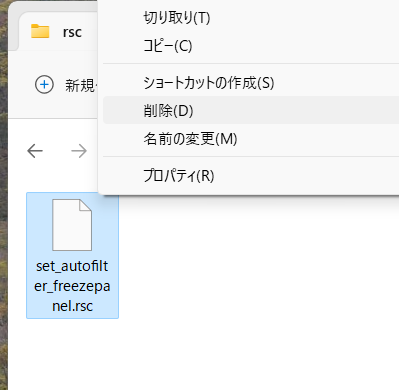
\includegraphics[width=0.3\textwidth,height=\textheight]{img/assoc_01.png}
\item
  拡張子が表示されていない場合は,エクスプローラの表示のオプションで,「登録されている拡張子は表示しない」のチェックを外して(チェックしないで),「OK」を選択してから,名前を変更する.\\
  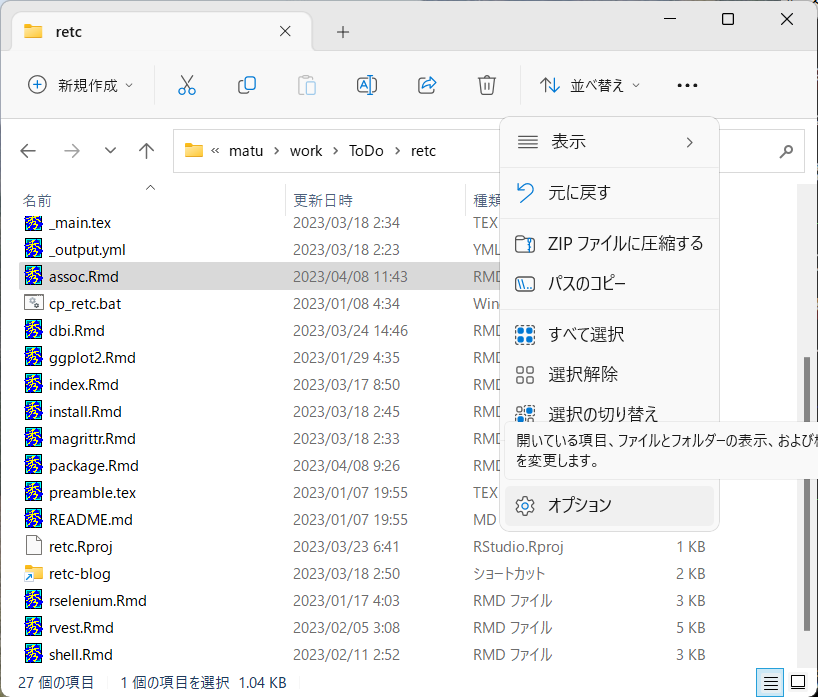
\includegraphics[width=0.4\textwidth,height=\textheight]{img/assoc_00_01.png}
  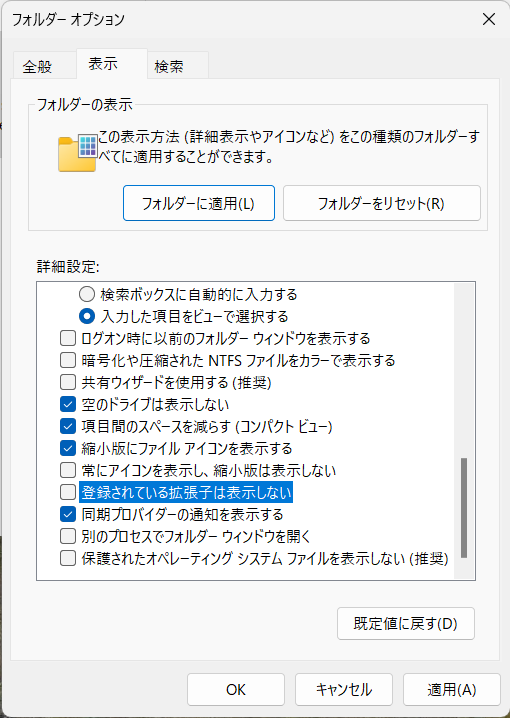
\includegraphics[width=0.4\textwidth,height=\textheight]{img/assoc_00_02.png}
\item
  ファイルを右クリックして,「プロパティ」を選択する.\\
  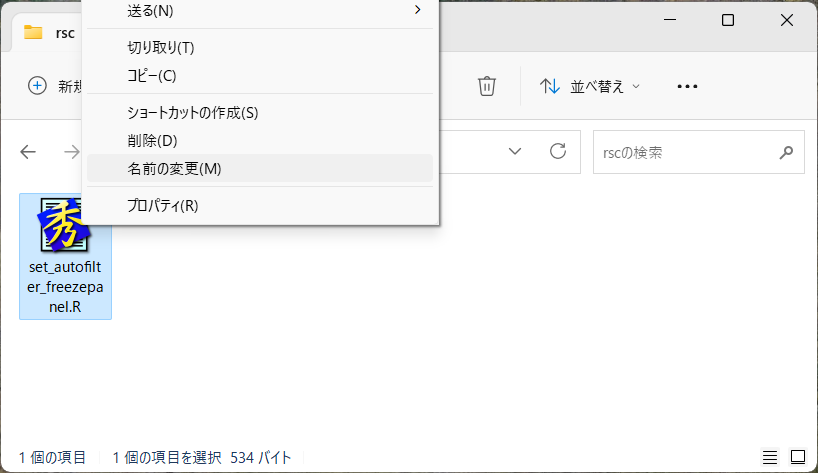
\includegraphics[width=0.3\textwidth,height=\textheight]{img/assoc_02.png}
\item
  「全般」タブのやや上にあるプログラムの「変更」を選択する.\\
  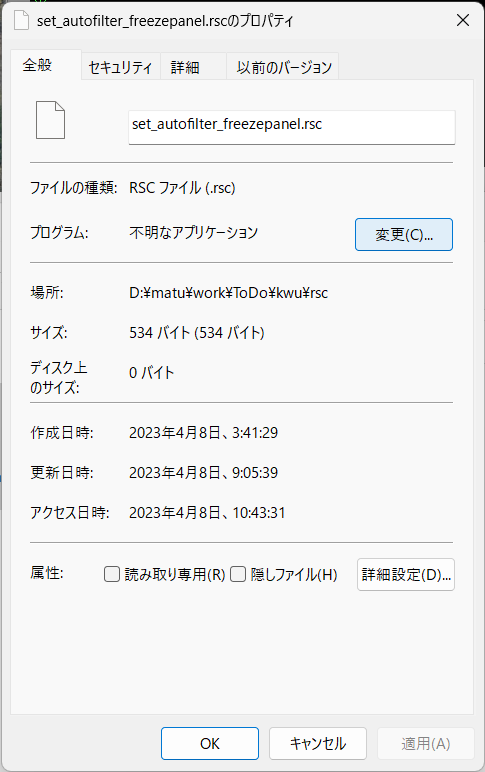
\includegraphics[width=0.5\textwidth,height=\textheight]{img/assoc_03.png}
\item
  「PCでアプリを選択する」をクリックする.\\
  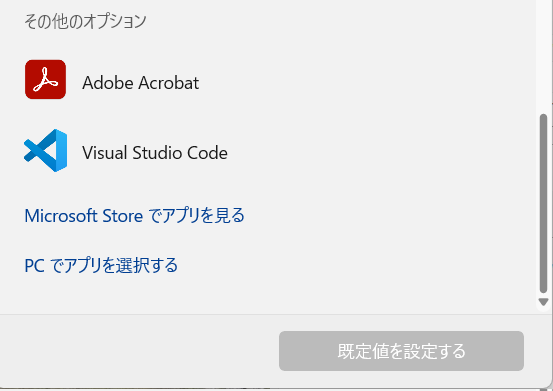
\includegraphics[width=0.5\textwidth,height=\textheight]{img/assoc_04.png}
\item
  ファイル選択画面で,Rをインストールしたフォルダまで辿っていき(「c:\textbackslash Program files\textbackslash R\textbackslash R-4.2.3\textbackslash bin\textbackslash x64」など),「Rscript.exe」を選択する.\\
  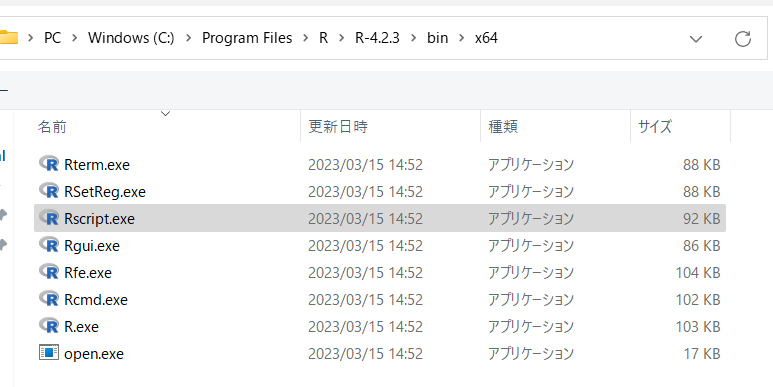
\includegraphics[width=0.5\textwidth,height=\textheight]{img/assoc_05.png}
\item
  「.rscファイルの既定のアプリを選択する」で「R for windows front-end」が表示されるので,「既定値を設定する」を選択する.\\
  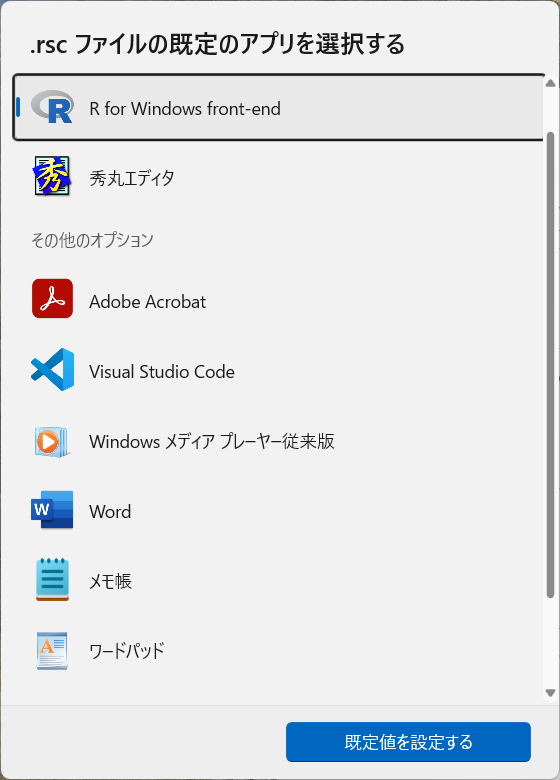
\includegraphics[width=0.5\textwidth,height=\textheight]{img/assoc_06.png}
\item
  全般タブのプログラムが「R for windows front-end」になっていることを確認して.「OK」を選択する.\\
  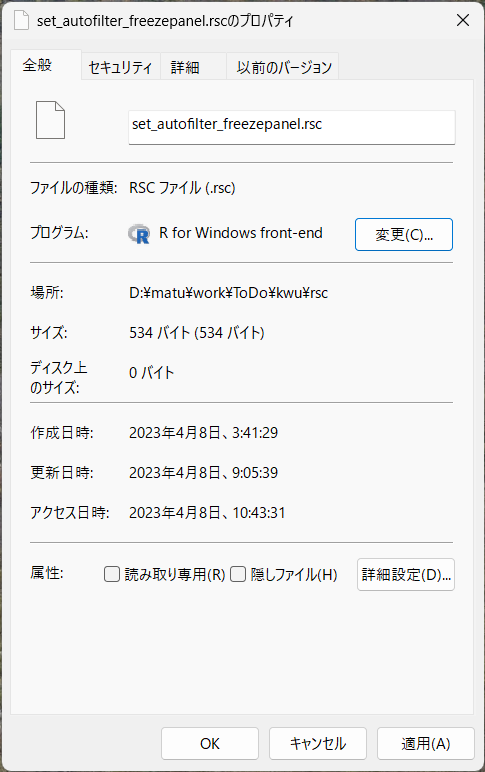
\includegraphics[width=0.5\textwidth,height=\textheight]{img/assoc_07.png}
\item
  ファイルのアイコンがRのアイコンになっていたらOKである.\\
  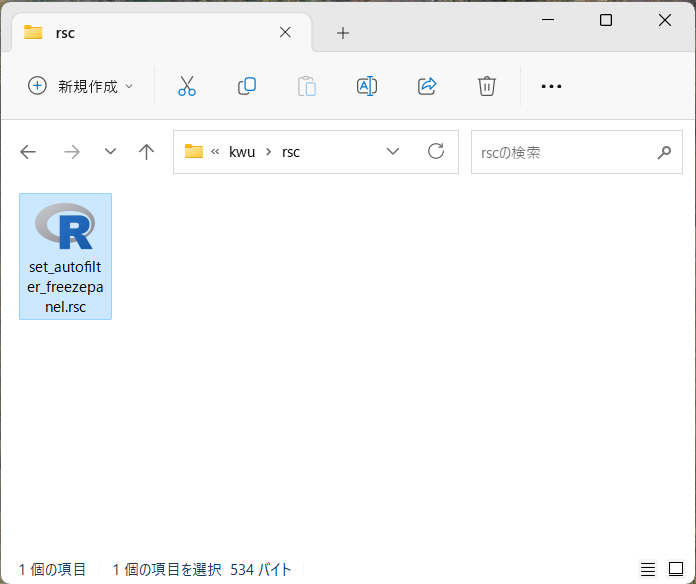
\includegraphics[width=0.3\textwidth,height=\textheight]{img/assoc_08.png}
\end{enumerate}

ダブルクリックすると,ファイルの内容が実行される(はず).

\hypertarget{macux3068linux}{%
\subsection{MacとLinux}\label{macux3068linux}}

MacでRのスクリプトファイルを簡単に実行するには以下の方法がある.

\begin{itemize}
\tightlist
\item
  plot.R などの名前でRのコードを保存\\
\item
  シェルスクリプトのファイル(例:plot.sh)を用意\\
\item
  plot.sh をクリックして実行
\end{itemize}

簡単な例として散布図をpdfに保存するコードを取り上げる.
次のコードをRで実行すると,乱数(x軸:一様分布,y軸:正規分布)に基づく散布図がpdfとして保存される.

\begin{Shaded}
\begin{Highlighting}[]
\CommentTok{\# コード例}
  \CommentTok{\# ユーザディレクトリにtest.pdfというファイルを生成}
\FunctionTok{pdf}\NormalTok{(}\StringTok{"\textasciitilde{}/test.pdf"}\NormalTok{)}
  \FunctionTok{plot}\NormalTok{(}\DecValTok{1}\NormalTok{, }\DecValTok{1}\NormalTok{)}
\FunctionTok{dev.off}\NormalTok{()}
\end{Highlighting}
\end{Shaded}

\includegraphics{assoc_files/figure-latex/unnamed-chunk-2-1.pdf}

このコードをユーザ・ディレクトリ(\textasciitilde/)に保存する.
ファイル名は何でも良いが,ここではplot.Rとする.

次に,plot.Rを実行するためのシェルスクリプトを作成する.
このファイル名も何でも良いが,ここではplot.shとする.
もちろん,Rと別のファイル名でも構わない.
plot.shの中身は次のようにする.

\begin{verbatim}
#! /bin/bash
/usr/local/bin/Rscript ~/plot.R
\end{verbatim}

\texttt{\#!}ではじまる1行目はシバンとよばれるもので,ある種のおまじないである.
\texttt{/bin/bash}というシェルで実行せよという意味である.
2行目の\texttt{/usr/local/bin/Rscript}は\texttt{Rscript}というプログラムを実行する部分である.
Rをインストールすると,\texttt{/usr/local/bin/}か\texttt{/usr/bin/}のどちらかに\texttt{Rscript}というプログラムが保存されている.
どちらに保存されているかは,そのときの設定によると思われるが,読者の環境に合わせる.

\texttt{\textasciitilde{}/plot.R}の部分は実行するRのコードのファイルを指定する.
他のファイルを実行する場合は,この部分を変更する.

これで準備が完了したので,\texttt{plot.sh}をクリックすれば\texttt{plot.R}がRscriptで実行され,\texttt{plot.pdf}を生成するはずである.
うまくいかなければ,\texttt{plot.sh}に実行権限が設定されていないことが考えられる.
Terminalから\texttt{plot.sh}のあるディレクトリで以下のように実行すれば,実行権限を設定する.

\begin{verbatim}
chmod +x plot.sh
\end{verbatim}

Linuxでも同様の方法で実行できるようになるはずである.

\hypertarget{magrittr}{%
\section{magrittrでコードを簡潔に}\label{magrittr}}

パッケージmagrittrはちょっと変わったパッケージである.
そもそも名前が変わっていて何と読んで良いのか分からない.
公式ページには「magrittr (to be pronounced with a sophisticated french accent) 」と書かれている.
フランス語は,大学の第2外国語で習ったが,すでに記憶の彼方に沈んでしまっている.
主な関数がパイプ(\texttt{\%\textgreater{}\%})である点も変わっている.

このように,ちょっと変わったパーッケージではあるものの,Rを使う際には欠かせないパッケージといっても過言ではない.
Rのバージョン4.1以降では,base機能のパイプとして\texttt{\textbar{}\textgreater{}}が使えるようになったが,第1引数(\texttt{\_})とその名前を明示しないといけないなど若干使いにくい.
そこでここでは,コードを簡潔に書くためのmagrittrのパイプ(\texttt{\%\textgreater{}\%})と関連した関数を紹介する.

\hypertarget{ux6e96ux5099}{%
\subsection{準備}\label{ux6e96ux5099}}

例によって,インストールとパッケージの呼び出しをしておく.

\begin{Shaded}
\begin{Highlighting}[]
\FunctionTok{install.packages}\NormalTok{(}\StringTok{"magrittr"}\NormalTok{)}
\end{Highlighting}
\end{Shaded}

\begin{Shaded}
\begin{Highlighting}[]
\FunctionTok{library}\NormalTok{(tidyverse)}
\FunctionTok{library}\NormalTok{(magrittr)}
\end{Highlighting}
\end{Shaded}

\hypertarget{magrittrux3068tidyverse}{%
\subsection{magrittrとtidyverse}\label{magrittrux3068tidyverse}}

tidyverseは,Rでのデータ解析には欠かせないものになっている.
Rの起動時にtidyverseを読み込む人は多いだろう.
tidyverseを読み込むと,その中のパッケージ(forcats,tibble,stringr,dplyr,tidyr,purrr)がインポートした\texttt{\%\textgreater{}\%}を使うことができる.
そのため,私は\texttt{\%\textgreater{}\%}がtidyverseの独自のものだと勘違いをしていた.
\texttt{\%\textgreater{}\%}はもとはパッケージmagrittrの関数である.

ただし,tidyverseと\texttt{\%\textgreater{}\%}の相性は非常によい.
tidyverseの関数では,第1引数のオブジェクトがdplyrではデータフレーム,stringrでは文字列などのように,それぞれのパッケージで引数とするオブジェクトが統一されている.
そのため,簡潔にコードを書くことができる.
なお,パイプの手入力は手間がかかるので,ショートカットを利用する.
RStudioでは,Ctrl + Shift + Mである.
テキストエディタを使っているときはマクロやスクリプトを組んでショートカットを設定することをお勧めする.

\texttt{\%\textgreater{}\%}は,慣れるまでは何が便利なのか分からないが,慣れると欠かせなくなる.
さらに使っていると,癖なってしまって無駄にパイプを繋ぐこともある.
長過ぎるパイプは良くないのは当然であるものの,適度に使うとRでのプログラミングは非常に楽になる.

\hypertarget{ux3067ux30b3ux30fcux30c9ux3092ux7c21ux6f54ux306b}{%
\subsection{\texorpdfstring{\texttt{\%\textgreater{}\%}でコードを簡潔に}{\%\textgreater\%でコードを簡潔に}}\label{ux3067ux30b3ux30fcux30c9ux3092ux7c21ux6f54ux306b}}

最近のRでは,パイプ(\texttt{\%\textgreater{}\%})を多用したコードをよく目にする.
はじめてみると,面食らって思考停止に陥ってしまうかも知れない.
しかし,恐れることはない.
以下では簡単な例を使って説明する.

\begin{Shaded}
\begin{Highlighting}[]
\NormalTok{a }\OtherTok{\textless{}{-}}\NormalTok{ a }\SpecialCharTok{\%\textgreater{}\%} \FunctionTok{fun}\NormalTok{() }\CommentTok{\# あるとき:慣れていないと変な感じ}
\NormalTok{a }\OtherTok{\textless{}{-}} \FunctionTok{fun}\NormalTok{(a)      }\CommentTok{\# ないとき:こっちのほうが分かりやすい}
\end{Highlighting}
\end{Shaded}

ある時とない時と比べると,ある時の方がコードが長くなっていて,何が便利なのかわからないだろう.
著者も正直なところ,少し見たときには便利さが全くわからなかった.

\begin{Shaded}
\begin{Highlighting}[]
  \CommentTok{\# ないとき:「a \textless{}{-} 」が何度も必要}
\NormalTok{a }\OtherTok{\textless{}{-}} \FunctionTok{fun1}\NormalTok{(a)}
\NormalTok{a }\OtherTok{\textless{}{-}} \FunctionTok{fun2}\NormalTok{(a)}
\NormalTok{a }\OtherTok{\textless{}{-}} \FunctionTok{fun3}\NormalTok{(a)}
  \CommentTok{\# 力技!:括弧が見づらい}
\NormalTok{a }\OtherTok{\textless{}{-}} \FunctionTok{fun3}\NormalTok{(}\FunctionTok{fun2}\NormalTok{(}\FunctionTok{fun1}\NormalTok{(a)))}
  \CommentTok{\# あるとき}
\NormalTok{a }\OtherTok{\textless{}{-}}\NormalTok{ a }\SpecialCharTok{\%\textgreater{}\%}   \CommentTok{\# aに(以下の結果を)代入}
  \FunctionTok{fun1}\NormalTok{() }\SpecialCharTok{\%\textgreater{}\%} \CommentTok{\# fun1を実行}
  \FunctionTok{fun2}\NormalTok{() }\SpecialCharTok{\%\textgreater{}\%} \CommentTok{\# fun2を実行}
  \FunctionTok{fun3}\NormalTok{() }\SpecialCharTok{\%\textgreater{}\%} \CommentTok{\# fun3を実行}
\end{Highlighting}
\end{Shaded}

パイプを使うと,左側のオブジェクトを右側の関数の第1引数として使うため,引数が1つだけの場合は引数を書く必要がなくなる.
このようにオブジェクトaに対して, fun1,fun2,fun3と順に関数を適用するということは,しばしば出てくる.
特に,dplyrで\texttt{select()},\texttt{filter()},\texttt{group\_by()},\texttt{summarise()}などを使う時はそうである.
その時,代入先のオブジェクト名を1回ずつ新たに考えるのは,非常に面倒である.
どこまでを同じ変数名として,どこで変えるかなど考えるのは手間だ.
キーボードでの打ち込みが多いほど,オブジェクト名の重複や入力間違いが発生する可能性が高くなり,バグの温床である.
これを避ける方法は入れ子状に書くことであるが,括弧の対応がよくわからず頭が混乱する.
正直なところ,著者は時々このようなコードを書くことがある.
しかし,他人から見たらこんな馬鹿げて見にくいコードは無い.

パイプを使うと,これらの問題が解決する.
また,見た目にもわかりやすくコードの再利用もしやすい利点もある.
見た目では,1つの作業が1行にあるため,可読性が高く人間の思考回路にも近い.
再利用するときに,処理対象のオブジェクトを引数として明記しなくても良いため,前後の文脈に左右されずに必要な部分のコードだけを複写・貼付できる.
慣れるには,ほんの少しの時間がかかるかもしれないが,ぜひとも活用してほしい.

\hypertarget{ux30d1ux30a4ux30d7ux306eux4ef2ux9593}{%
\subsection{パイプの仲間}\label{ux30d1ux30a4ux30d7ux306eux4ef2ux9593}}

\begin{itemize}
\tightlist
\item
  \texttt{\%\textless{}\textgreater{}\%}\strut \\
\item
  \texttt{\%T\textgreater{}\%}(Tパイプというらしい)\\
\item
  \texttt{\%\$\%}
\end{itemize}

これらの関数は,tidyverseには含まれていないため,使用するにはmagrittrを読み込む必要がある.
\texttt{\%\textgreater{}\%}と似た機能を持つ.

\hypertarget{ux3067ux30aaux30d6ux30b8ux30a7ux30afux30c8ux3092ux4ee3ux5165}{%
\subsubsection{\texorpdfstring{\texttt{\%\textless{}\textgreater{}\%}でオブジェクトを代入}{\%\textless\textgreater\%でオブジェクトを代入}}\label{ux3067ux30aaux30d6ux30b8ux30a7ux30afux30c8ux3092ux4ee3ux5165}}

\texttt{\%\textless{}\textgreater{}\%}は,パイプを使って処理した内容を,最初のオブジェクトに再度代入するときに使う.
ほんの少しだけ,コードを短くできる.

\begin{Shaded}
\begin{Highlighting}[]
\FunctionTok{head}\NormalTok{(mpg) }\CommentTok{\# 燃費データ}
\end{Highlighting}
\end{Shaded}

\begin{verbatim}
## # A tibble: 6 x 11
##   manufacturer model displ  year   cyl trans      drv     cty   hwy fl    class 
##   <chr>        <chr> <dbl> <int> <int> <chr>      <chr> <int> <int> <chr> <chr> 
## 1 audi         a4      1.8  1999     4 auto(l5)   f        18    29 p     compa~
## 2 audi         a4      1.8  1999     4 manual(m5) f        21    29 p     compa~
## 3 audi         a4      2    2008     4 manual(m6) f        20    31 p     compa~
## 4 audi         a4      2    2008     4 auto(av)   f        21    30 p     compa~
## 5 audi         a4      2.8  1999     6 auto(l5)   f        16    26 p     compa~
## 6 audi         a4      2.8  1999     6 manual(m5) f        18    26 p     compa~
\end{verbatim}

\begin{Shaded}
\begin{Highlighting}[]
\NormalTok{tmp }\OtherTok{\textless{}{-}}\NormalTok{ mpg}
\NormalTok{tmp }\OtherTok{\textless{}{-}}
\NormalTok{  tmp }\SpecialCharTok{\%\textgreater{}\%}
\NormalTok{  dplyr}\SpecialCharTok{::}\FunctionTok{filter}\NormalTok{(year}\SpecialCharTok{==}\DecValTok{1999}\NormalTok{) }\SpecialCharTok{\%\textgreater{}\%}
\NormalTok{  tidyr}\SpecialCharTok{::}\FunctionTok{separate}\NormalTok{(trans, }\AttributeTok{into=}\FunctionTok{c}\NormalTok{(}\StringTok{"trans1"}\NormalTok{, }\StringTok{"trans2"}\NormalTok{, }\ConstantTok{NA}\NormalTok{))}

\NormalTok{tmp }\OtherTok{\textless{}{-}}\NormalTok{ mpg}
\NormalTok{tmp }\SpecialCharTok{\%\textless{}\textgreater{}\%}
\NormalTok{  dplyr}\SpecialCharTok{::}\FunctionTok{filter}\NormalTok{(year}\SpecialCharTok{==}\DecValTok{1999}\NormalTok{) }\SpecialCharTok{\%\textgreater{}\%}
\NormalTok{  tidyr}\SpecialCharTok{::}\FunctionTok{separate}\NormalTok{(trans, }\AttributeTok{into=}\FunctionTok{c}\NormalTok{(}\StringTok{"trans1"}\NormalTok{, }\StringTok{"trans2"}\NormalTok{, }\ConstantTok{NA}\NormalTok{))}
\end{Highlighting}
\end{Shaded}

注意点としては,試行錯誤でコードを書いている途中は,あまり使わないほうが良いだろう.
もとのオブジェクトが置き換わるので,処理結果が求めるものでないときに,もとに戻れなくなってしまうためだ.
コードを短くできるのは1行で,可読性が特に高くなるというわけでもない.
便利なことは便利で,私も一時期はよく使用していた.
しかし,上記の理由もあって,最近はほとんど使用していない.

\hypertarget{tux3067ux30b3ux30fcux30c9ux3092ux5206ux5c90}{%
\subsubsection{\texorpdfstring{\texttt{\%T\textgreater{}\%}でコードを分岐}{\%T\textgreater\%でコードを分岐}}\label{tux3067ux30b3ux30fcux30c9ux3092ux5206ux5c90}}

処理途中に分岐をして別の処理をさせたいときに使う.
例えば,ちょっとだけ処理して,変数に保存するときに使う.
imapと組み合わせて,保存する画像のファイル名を設定する時に使うと便利である.

\texttt{\%T\textgreater{}\%}は便利ではあるが,以下の点で注意が必要である.

\begin{itemize}
\tightlist
\item
  分岐途中の結果をオブジェクトに代入するときには,\texttt{\textless{}-}ではなく,\texttt{\textless{}\textless{}-}を使う\\
\item
  明示的に\texttt{.}を使う\\
\item
  複数処理があれば,\texttt{\{}と\texttt{\}}で囲う\\
\item
  処理終了後に\texttt{\%\textgreater{}\%}が必要
\end{itemize}

\texttt{\%T\textgreater{}\%}を使うとコードの途中に,ちょっとだけ枝分かれしたコードを挿入できる.
有用な機能ではあるが,トリッキーなコードになる可能性があるため,使いすぎには気をつけたい.

以下の例は,あまり実用的なものではないが,簡単な例として示す.

\begin{Shaded}
\begin{Highlighting}[]
\NormalTok{iris }\SpecialCharTok{\%\textgreater{}\%}
\NormalTok{  tibble}\SpecialCharTok{::}\FunctionTok{tibble}\NormalTok{() }\SpecialCharTok{\%\textgreater{}\%}
  \FunctionTok{split}\NormalTok{(.}\SpecialCharTok{$}\NormalTok{Species) }\SpecialCharTok{\%\textgreater{}\%}          \CommentTok{\# Speciesで分割}
\NormalTok{  purrr}\SpecialCharTok{::}\FunctionTok{map}\NormalTok{(print, }\AttributeTok{n =} \DecValTok{3}\NormalTok{) }\SpecialCharTok{\%T\textgreater{}\%} \CommentTok{\# それぞれ3行だけ表示}
\NormalTok{  \{}
\NormalTok{    sp\_path }\OtherTok{\textless{}\textless{}{-}} \FunctionTok{paste0}\NormalTok{(}\FunctionTok{names}\NormalTok{(.), }\StringTok{".txt"}\NormalTok{) }\CommentTok{\# ファイル名:種名.txt}
\NormalTok{  \} }\SpecialCharTok{\%\textgreater{}\%}
\NormalTok{  purrr}\SpecialCharTok{::}\FunctionTok{map}\NormalTok{(dplyr}\SpecialCharTok{::}\NormalTok{select\_if, is.numeric) }\SpecialCharTok{\%\textgreater{}\%} \CommentTok{\# 数値だけを選択}
\NormalTok{  purrr}\SpecialCharTok{::}\FunctionTok{map}\NormalTok{(dplyr}\SpecialCharTok{::}\NormalTok{summarise\_all, mean) }\SpecialCharTok{\%\textgreater{}\%}   \CommentTok{\# 平均を算出}
\NormalTok{  purrr}\SpecialCharTok{::}\FunctionTok{map2}\NormalTok{(}\AttributeTok{.x =}\NormalTok{ ., }\AttributeTok{.y =}\NormalTok{ sp\_path, readr}\SpecialCharTok{::}\NormalTok{write\_csv) }\CommentTok{\# 種ごとにcsvを保存}
\end{Highlighting}
\end{Shaded}

Tパイプは,Tの文字の形が意味をなしており,左から来たデータを分岐させて右側と下側に流す役割をする.
上の例では,分岐した途中でファイル名\texttt{sp\_path}を生成するために,(わざと)分岐を入れている.
このコードで本来\texttt{\{\}}は不要だが,入れておくとTパイプを使っている部分がわかりやすい.
ファイル名を生成したあと(\texttt{\}}の後ろ)には,上から流れてきたものがそのまま\texttt{purrr::map()}の第1引数として使われる.
\texttt{select\_if()}と\texttt{dplyr::summarise\_all()}をしてから,最終的にファイルとして出力する.
\texttt{map2()}は\texttt{map()}の引数を2つとるバージョンであり,第1引数に上から来たデータフレームを,第2引数にファイル名を使っている.

なお,最後の\texttt{map2()}を\texttt{purrr::walk2}とすると種ごとの平均値は画面には出力されず,ファイルへの出力だけになる.
さらに余談だが,上で「(わざと)」と書いたのは,Tパイプを使わずに,最後のところを\texttt{map2(.x\ =\ .,\ .y\ =\ paste0(names(.),\ ".txt"),\ readr::write\_csv)}とすれば同じ結果が得られるためである.

\begin{Shaded}
\begin{Highlighting}[]
\NormalTok{iris }\SpecialCharTok{\%\textgreater{}\%}
\NormalTok{  tibble}\SpecialCharTok{::}\FunctionTok{tibble}\NormalTok{() }\SpecialCharTok{\%\textgreater{}\%}
  \FunctionTok{split}\NormalTok{(.}\SpecialCharTok{$}\NormalTok{Species) }\SpecialCharTok{\%\textgreater{}\%}
\NormalTok{  purrr}\SpecialCharTok{::}\FunctionTok{map}\NormalTok{(dplyr}\SpecialCharTok{::}\NormalTok{select\_if, is.numeric) }\SpecialCharTok{\%\textgreater{}\%}
\NormalTok{  purrr}\SpecialCharTok{::}\FunctionTok{map}\NormalTok{(dplyr}\SpecialCharTok{::}\NormalTok{summarise\_all, mean) }\SpecialCharTok{\%\textgreater{}\%}
  \FunctionTok{map2}\NormalTok{(}\AttributeTok{.x =}\NormalTok{ ., }\AttributeTok{.y =} \FunctionTok{paste0}\NormalTok{(}\FunctionTok{names}\NormalTok{(.), }\StringTok{".txt"}\NormalTok{), readr}\SpecialCharTok{::}\NormalTok{write\_csv)}
\end{Highlighting}
\end{Shaded}

\hypertarget{ux3067ux306eux30b7ux30e7ux30fcux30c8ux30abux30c3ux30c8}{%
\subsubsection{\texorpdfstring{\texttt{\%\$\%}で\texttt{\$}のショートカット}{\%\$\%で\$のショートカット}}\label{ux3067ux306eux30b7ux30e7ux30fcux30c8ux30abux30c3ux30c8}}

\texttt{\%\$\%}は,\texttt{\%\textgreater{}\%}と\texttt{.\$}の組み合わせのショートカットである.

\begin{Shaded}
\begin{Highlighting}[]
\NormalTok{mpg }\SpecialCharTok{\%\textgreater{}\%}\NormalTok{ .}\SpecialCharTok{$}\NormalTok{manufacturer }\SpecialCharTok{\%\textgreater{}\%} \FunctionTok{head}\NormalTok{()}
\end{Highlighting}
\end{Shaded}

\begin{verbatim}
## [1] "audi" "audi" "audi" "audi" "audi" "audi"
\end{verbatim}

\begin{Shaded}
\begin{Highlighting}[]
\NormalTok{mpg }\SpecialCharTok{\%$\%}\NormalTok{   manufacturer }\SpecialCharTok{\%\textgreater{}\%} \FunctionTok{head}\NormalTok{()}
\end{Highlighting}
\end{Shaded}

\begin{verbatim}
## [1] "audi" "audi" "audi" "audi" "audi" "audi"
\end{verbatim}

パッケージ開発ではパイプを使った場合の\texttt{.}が推奨されていない.
パッケージ開発時に欠かせないチェック(R CMD check)ではpossible problemとしてWarningが出力される.
そのため,そのままではCRANでは受け付けてもらえない.
Githubでパッケージを公開するならそれでも問題はないが,Checkで毎回Warningが出力されるのは,心理的に嬉しくない.

そこで,DESCRIPTIONで次のように\texttt{\%\$\%}をインポートしておくと,\texttt{.\$}を使わなくても良い.

\begin{Shaded}
\begin{Highlighting}[]
\FunctionTok{importFrom}\NormalTok{(magrittr,}\StringTok{"\%$\%"}\NormalTok{)}
\end{Highlighting}
\end{Shaded}

なお余談ではあるが,この場合は\texttt{\$}の代わりに\texttt{{[}{[}}と\texttt{{]}{]}}を使っても同じ結果が得られる.
\texttt{{[}}と\texttt{{]}}ではデータフレームの1列をそのまま取り出すので,結果が異なる.

\begin{Shaded}
\begin{Highlighting}[]
\NormalTok{mpg }\SpecialCharTok{\%\textgreater{}\%}\NormalTok{ .}\SpecialCharTok{$}\NormalTok{manufacturer      }\SpecialCharTok{\%\textgreater{}\%} \FunctionTok{head}\NormalTok{()}
\end{Highlighting}
\end{Shaded}

\begin{verbatim}
## [1] "audi" "audi" "audi" "audi" "audi" "audi"
\end{verbatim}

\begin{Shaded}
\begin{Highlighting}[]
\NormalTok{mpg }\SpecialCharTok{\%\textgreater{}\%}\NormalTok{ .[[}\StringTok{"manufacturer"}\NormalTok{]] }\SpecialCharTok{\%\textgreater{}\%} \FunctionTok{head}\NormalTok{()}
\end{Highlighting}
\end{Shaded}

\begin{verbatim}
## [1] "audi" "audi" "audi" "audi" "audi" "audi"
\end{verbatim}

\begin{Shaded}
\begin{Highlighting}[]
\NormalTok{mpg }\SpecialCharTok{\%\textgreater{}\%}\NormalTok{ .[}\StringTok{"manufacturer"}\NormalTok{]   }\SpecialCharTok{\%\textgreater{}\%} \FunctionTok{head}\NormalTok{()}
\end{Highlighting}
\end{Shaded}

\begin{verbatim}
## # A tibble: 6 x 1
##   manufacturer
##   <chr>       
## 1 audi        
## 2 audi        
## 3 audi        
## 4 audi        
## 5 audi        
## 6 audi
\end{verbatim}

\texttt{{[}{[}\ {]}{]}}と\texttt{{[}\ {]}}は,それぞれ\texttt{{[}{[}}と\texttt{{[}}という関数であるため,以下のように書くことができる.
この場合,第1引数がパイプの前から引き継がれるため,\texttt{.}を明示しなくてもよい.

\begin{Shaded}
\begin{Highlighting}[]
\NormalTok{mpg }\SpecialCharTok{\%\textgreater{}\%} \StringTok{\textasciigrave{}}\AttributeTok{$}\StringTok{\textasciigrave{}}\NormalTok{(manufacturer)    }\SpecialCharTok{\%\textgreater{}\%} \FunctionTok{head}\NormalTok{()}
\end{Highlighting}
\end{Shaded}

\begin{verbatim}
## [1] "audi" "audi" "audi" "audi" "audi" "audi"
\end{verbatim}

\begin{Shaded}
\begin{Highlighting}[]
\NormalTok{mpg }\SpecialCharTok{\%\textgreater{}\%} \StringTok{\textasciigrave{}}\AttributeTok{[[}\StringTok{\textasciigrave{}}\NormalTok{(}\StringTok{"manufacturer"}\NormalTok{) }\SpecialCharTok{\%\textgreater{}\%} \FunctionTok{head}\NormalTok{() }\CommentTok{\# mpg \%\textgreater{}\% \textasciigrave{}[[\textasciigrave{}(., "manufacturer") と同じ}
\end{Highlighting}
\end{Shaded}

\begin{verbatim}
## [1] "audi" "audi" "audi" "audi" "audi" "audi"
\end{verbatim}

\begin{Shaded}
\begin{Highlighting}[]
\NormalTok{mpg }\SpecialCharTok{\%\textgreater{}\%} \StringTok{\textasciigrave{}}\AttributeTok{[}\StringTok{\textasciigrave{}}\NormalTok{(}\StringTok{"manufacturer"}\NormalTok{)  }\SpecialCharTok{\%\textgreater{}\%} \FunctionTok{head}\NormalTok{()}
\end{Highlighting}
\end{Shaded}

\begin{verbatim}
## # A tibble: 6 x 1
##   manufacturer
##   <chr>       
## 1 audi        
## 2 audi        
## 3 audi        
## 4 audi        
## 5 audi        
## 6 audi
\end{verbatim}

\hypertarget{ux30d1ux30a4ux30d7ux4ee5ux5916ux306eux95a2ux6570}{%
\subsection{パイプ以外の関数}\label{ux30d1ux30a4ux30d7ux4ee5ux5916ux306eux95a2ux6570}}

magrittrにはパイプとともに使うと便利な関数も含まれている.
例えば,パイプを使ったコードの中で列名を変更したいことがある.
\texttt{set\_colnames()}はデータフレームの列名を変更する時に便利だ.
これを使わずに列名を変更しようとすると,ちょっとトリッキーな関数\texttt{colnames\textless{}-()}を使うか,途中でコードを区切る必要がある.

\begin{Shaded}
\begin{Highlighting}[]
\NormalTok{hoge }\OtherTok{\textless{}{-}}\NormalTok{ dplyr}\SpecialCharTok{::}\FunctionTok{select}\NormalTok{(mpg, }\DecValTok{1}\SpecialCharTok{:}\DecValTok{2}\NormalTok{)}
\NormalTok{cnames }\OtherTok{\textless{}{-}} \FunctionTok{c}\NormalTok{(}\StringTok{"foo"}\NormalTok{, }\StringTok{"bar"}\NormalTok{)}
 \CommentTok{\# colnames(hoge) \textless{}{-} cnames      \# 通常のコード}
\StringTok{\textasciigrave{}}\AttributeTok{colnames\textless{}{-}}\StringTok{\textasciigrave{}}\NormalTok{(hoge, cnames)       }\CommentTok{\# トリッキーなコード}
\NormalTok{hoge }\SpecialCharTok{\%\textgreater{}\%} 
\NormalTok{  magrittr}\SpecialCharTok{::}\FunctionTok{set\_colnames}\NormalTok{(cnames)}
\end{Highlighting}
\end{Shaded}

\hypertarget{ux30b3ux30e9ux30e0magrittrux306eux4e0dux601dux8b70ux306aux95a2ux6570ux305fux3061}{%
\subsection{コラム:magrittrの不思議な関数たち}\label{ux30b3ux30e9ux30e0magrittrux306eux4e0dux601dux8b70ux306aux95a2ux6570ux305fux3061}}

magrittrは,そもそも変わったパッケージだが,不思議な名前の関数もある.

\begin{Shaded}
\begin{Highlighting}[]
\NormalTok{add          }\CommentTok{\# \textasciigrave{}+\textasciigrave{}}
\NormalTok{subtract     }\CommentTok{\# \textasciigrave{}{-}\textasciigrave{}}
\NormalTok{multiply\_by  }\CommentTok{\# \textasciigrave{}*\textasciigrave{}}
\NormalTok{divide\_by    }\CommentTok{\# \textasciigrave{}/\textasciigrave{}}
\end{Highlighting}
\end{Shaded}

\texttt{?not}とすれば,似たような不思議な関数の一覧と説明が出てくる.
特に四則演算をする関数の場合は,パイプと一緒に使うと若干だが読みやすい.
\texttt{+}と同じ機能である\texttt{add}であれば,以下のようになる.

\begin{Shaded}
\begin{Highlighting}[]
\DecValTok{1}\SpecialCharTok{:}\DecValTok{10} \SpecialCharTok{\%\textgreater{}\%} 
  \StringTok{\textasciigrave{}}\AttributeTok{+}\StringTok{\textasciigrave{}}\NormalTok{(}\DecValTok{100}\NormalTok{)}
\end{Highlighting}
\end{Shaded}

\begin{verbatim}
##  [1] 101 102 103 104 105 106 107 108 109 110
\end{verbatim}

\begin{Shaded}
\begin{Highlighting}[]
\DecValTok{1}\SpecialCharTok{:}\DecValTok{10} \SpecialCharTok{\%\textgreater{}\%} 
  \FunctionTok{add}\NormalTok{(}\DecValTok{100}\NormalTok{)}
\end{Highlighting}
\end{Shaded}

\begin{verbatim}
##  [1] 101 102 103 104 105 106 107 108 109 110
\end{verbatim}

パイプで使わない場合は,普通の四則演算の方がわかりやすい.

\begin{Shaded}
\begin{Highlighting}[]
\DecValTok{1}\SpecialCharTok{:}\DecValTok{10} \SpecialCharTok{+} \DecValTok{100}
\end{Highlighting}
\end{Shaded}

\begin{verbatim}
##  [1] 101 102 103 104 105 106 107 108 109 110
\end{verbatim}

\begin{Shaded}
\begin{Highlighting}[]
\FunctionTok{add}\NormalTok{(}\DecValTok{1}\SpecialCharTok{:}\DecValTok{10}\NormalTok{, }\DecValTok{100}\NormalTok{)}
\end{Highlighting}
\end{Shaded}

\begin{verbatim}
##  [1] 101 102 103 104 105 106 107 108 109 110
\end{verbatim}

論理演算で使う関数もパイプで使うと読みやすくなりそう.

\begin{Shaded}
\begin{Highlighting}[]
\NormalTok{and          }\CommentTok{\# \textasciigrave{}\&\textasciigrave{}}
\NormalTok{or           }\CommentTok{\# \textasciigrave{}|\textasciigrave{}}
\NormalTok{equals       }\CommentTok{\# \textasciigrave{}==\textasciigrave{}}
\NormalTok{not          }\CommentTok{\# \textasciigrave{}!\textasciigrave{},\textasciigrave{}n\textquotesingle{}est pas\textasciigrave{}(フランス語)も同じ}
\end{Highlighting}
\end{Shaded}

\texttt{\&}や\texttt{\textbar{}}で,条件が多くなってくると読みにくくなるので,改行するかパイプで繋いで1つ1つの条件を短くするとコードが読みやすくなる.

\begin{Shaded}
\begin{Highlighting}[]
\FunctionTok{rep}\NormalTok{(}\FunctionTok{c}\NormalTok{(}\ConstantTok{TRUE}\NormalTok{, }\ConstantTok{FALSE}\NormalTok{), }\AttributeTok{times =} \DecValTok{5}\NormalTok{) }\SpecialCharTok{\%\textgreater{}\%}
  \FunctionTok{and}\NormalTok{(}\FunctionTok{rep}\NormalTok{(}\FunctionTok{c}\NormalTok{(}\ConstantTok{TRUE}\NormalTok{, }\ConstantTok{FALSE}\NormalTok{), }\AttributeTok{each =} \DecValTok{5}\NormalTok{))}
\end{Highlighting}
\end{Shaded}

\begin{verbatim}
##  [1]  TRUE FALSE  TRUE FALSE  TRUE FALSE FALSE FALSE FALSE FALSE
\end{verbatim}

\begin{Shaded}
\begin{Highlighting}[]
\FunctionTok{rep}\NormalTok{(}\FunctionTok{c}\NormalTok{(}\ConstantTok{TRUE}\NormalTok{, }\ConstantTok{FALSE}\NormalTok{), }\AttributeTok{times =} \DecValTok{5}\NormalTok{) }\SpecialCharTok{\%\textgreater{}\%}
  \FunctionTok{or}\NormalTok{(}\FunctionTok{rep}\NormalTok{(}\FunctionTok{c}\NormalTok{(}\ConstantTok{TRUE}\NormalTok{, }\ConstantTok{FALSE}\NormalTok{), }\AttributeTok{each =} \DecValTok{5}\NormalTok{))}
\end{Highlighting}
\end{Shaded}

\begin{verbatim}
##  [1]  TRUE  TRUE  TRUE  TRUE  TRUE FALSE  TRUE FALSE  TRUE FALSE
\end{verbatim}

\hypertarget{tidyverse}{%
\section{tidyverseを使う}\label{tidyverse}}

\hypertarget{ux6e96ux5099-1}{%
\subsection{準備}\label{ux6e96ux5099-1}}

\begin{Shaded}
\begin{Highlighting}[]
\FunctionTok{install.packages}\NormalTok{(}\StringTok{"tidyverse"}\NormalTok{)}
\end{Highlighting}
\end{Shaded}

\begin{Shaded}
\begin{Highlighting}[]
\FunctionTok{library}\NormalTok{(tidyverse)}
\end{Highlighting}
\end{Shaded}

\hypertarget{tidyverseux3068ux306f}{%
\subsection{tidyverseとは}\label{tidyverseux3068ux306f}}

tidyverseは単一のパッケージではなく,9つのパッケージを含むパッケージ群である.

\begin{itemize}
\tightlist
\item
  tibble:データフレームの拡張型
\item
  tidyr:整然(tidy)データのツール
\item
  readr:ファイル読み込み・保存
\item
  dplyr:データフレーム操作
\item
  stringr:文字列
\item
  purrr:繰り返し処理
\item
  ggplot2:作図
\item
  lubridate:日付・時間データ
\item
  forcats:ファクター(因子)操作
\end{itemize}

このうち,この文書ではファクター(因子)をほとんど扱っていないため,forcatsについては説明しない.
ggplot2とlubridateはそれぞれ第?章と第?章で説明し,その他はこの章で説明する.

\hypertarget{tibbleux3067ux30c7ux30fcux30bfux30d5ux30ecux30fcux30e0ux3092ux4f7fux3044ux3084ux3059ux304fux3059ux308b}{%
\subsection{tibbleでデータフレームを使いやすくする}\label{tibbleux3067ux30c7ux30fcux30bfux30d5ux30ecux30fcux30e0ux3092ux4f7fux3044ux3084ux3059ux304fux3059ux308b}}

\hypertarget{ux30c7ux30fcux30bfux30d5ux30ecux30fcux30e0ux3068tibble}{%
\subsubsection{データフレームとtibble}\label{ux30c7ux30fcux30bfux30d5ux30ecux30fcux30e0ux3068tibble}}

tidyvrseでは,データフレーム(data.frame)をさらに拡張して使いやすくした tbl\_dfやtblという形式を基本的に使う.
ふつうに使っている限りはそれほど大きな違いはない.
違いないというよりも,オブジェクト名そのものや\texttt{print()}で内容を表示させたときに見やすいという利点がある.
例えば,各列のデータのタイプが表示される.
int(整数)やchr(文字列)のように省略して表示されるので,若干の慣れが必要である.

\hypertarget{tibbleux306eux6c17ux306eux5229ux3044ux305fux8868ux793a}{%
\subsubsection{tibbleの気の利いた表示}\label{tibbleux306eux6c17ux306eux5229ux3044ux305fux8868ux793a}}

画面の幅に表示を合わせてくれるのも良い点である.
例えば,次のように画面の幅に収まりきらない場合でも,データフレームではダラダラと表示を続ける.
一方,tibbleでは画面の幅に入る範囲に「良い感じ」にまとめて表示してくれる.
それでも表示できなかった場合は,最後に列名とその形式を出力する.

\begin{Shaded}
\begin{Highlighting}[]
\NormalTok{n }\OtherTok{\textless{}{-}} \DecValTok{3}
\NormalTok{ncol }\OtherTok{\textless{}{-}} \DecValTok{10}
\NormalTok{cnames }\OtherTok{\textless{}{-}}\NormalTok{ letters[}\FunctionTok{seq}\NormalTok{(ncol)]}
\NormalTok{df }\OtherTok{\textless{}{-}} 
  \FunctionTok{matrix}\NormalTok{(}\FunctionTok{rnorm}\NormalTok{(n }\SpecialCharTok{*}\NormalTok{ ncol), }\AttributeTok{ncol =}\NormalTok{ ncol, }\AttributeTok{dimnames =} \FunctionTok{list}\NormalTok{(}\FunctionTok{seq}\NormalTok{(n), cnames)) }\SpecialCharTok{\%\textgreater{}\%}
  \FunctionTok{as.data.frame}\NormalTok{() }\SpecialCharTok{\%\textgreater{}\%}
  \FunctionTok{print}\NormalTok{()}
\end{Highlighting}
\end{Shaded}

\begin{verbatim}
##            a          b          c          d          e           f          g
## 1 -1.3135848  0.3258321  0.6286094  0.8868641  0.9018192  0.81154500 -0.1813681
## 2  0.6630295 -0.1539541  0.5292270 -0.6665338 -1.0718088 -0.02525752  0.5337847
## 3 -0.5375106  1.6347028 -0.2873361  0.3141193 -0.3897252  0.50563437  1.0686319
##           h           i          j
## 1 0.7282541 -0.03894795  1.0830392
## 2 1.0519735  1.41976184 -0.0658578
## 3 0.7313550  0.28444134  0.5333303
\end{verbatim}

\begin{Shaded}
\begin{Highlighting}[]
\NormalTok{tibble}\SpecialCharTok{::}\FunctionTok{as\_tibble}\NormalTok{(df)}
\end{Highlighting}
\end{Shaded}

\begin{verbatim}
## # A tibble: 3 x 10
##        a      b      c      d      e       f      g     h       i       j
##    <dbl>  <dbl>  <dbl>  <dbl>  <dbl>   <dbl>  <dbl> <dbl>   <dbl>   <dbl>
## 1 -1.31   0.326  0.629  0.887  0.902  0.812  -0.181 0.728 -0.0389  1.08  
## 2  0.663 -0.154  0.529 -0.667 -1.07  -0.0253  0.534 1.05   1.42   -0.0659
## 3 -0.538  1.63  -0.287  0.314 -0.390  0.506   1.07  0.731  0.284   0.533
\end{verbatim}

変なたとえかもしれないが,データフレームは「言われたことをそのままやりました」という何も考えずに与えられたことをするような感じで,tibbleは「見やすく修正しておきました」という非常に気の利いた対応をする感じである.

さらに,tibbleでは行数が多いときは最初の10行だけ表示する.
データフレームではすべてのデータを表示させるので,巨大なデータのときに,画面がやたらスクロールして困った経験があるかもしれない.
tibbleではそれがない.
なお,行数と列数は最初に書かれている.

\begin{Shaded}
\begin{Highlighting}[]
\NormalTok{n }\OtherTok{\textless{}{-}} \DecValTok{21}
\NormalTok{ncol }\OtherTok{\textless{}{-}} \DecValTok{3}
\NormalTok{cnames }\OtherTok{\textless{}{-}}\NormalTok{ letters[}\FunctionTok{seq}\NormalTok{(ncol)]}
\NormalTok{df }\OtherTok{\textless{}{-}} 
  \FunctionTok{matrix}\NormalTok{(}\FunctionTok{rnorm}\NormalTok{(n }\SpecialCharTok{*}\NormalTok{ ncol), }\AttributeTok{ncol =}\NormalTok{ ncol, }\AttributeTok{dimnames =} \FunctionTok{list}\NormalTok{(}\FunctionTok{seq}\NormalTok{(n), cnames)) }\SpecialCharTok{\%\textgreater{}\%}
  \FunctionTok{as.data.frame}\NormalTok{() }\SpecialCharTok{\%\textgreater{}\%}
  \FunctionTok{print}\NormalTok{()}
\end{Highlighting}
\end{Shaded}

\begin{verbatim}
##              a           b           c
## 1   0.35475882  0.98576502  1.85558063
## 2  -1.33862666  0.95126894  0.05442413
## 3   1.79033272  1.28345518  1.07043527
## 4  -1.32753696 -0.62237492 -0.33573553
## 5   0.82825839 -1.62273578 -1.72189442
## 6  -0.67056908 -0.81137801 -2.06298575
## 7   0.06586681  0.20062189  0.61980648
## 8  -0.01837473  0.59613173 -0.27851550
## 9  -0.91791524  0.74809545  0.74491957
## 10  0.43831650  0.09698700  0.33147597
## 11 -0.02769250 -0.53624010  0.39338219
## 12  1.30365379 -1.04999801 -0.46493327
## 13 -0.53412503 -0.18472232 -0.49193168
## 14 -0.82126141  0.23557813 -1.31723148
## 15 -1.57047874 -0.09585048 -2.05633368
## 16 -0.59443837  0.14927487  1.43406228
## 17 -0.52450623  1.61884642  0.13953113
## 18 -0.73447200  1.19052003  0.22625906
## 19  2.06498702  0.94910025  0.03473814
## 20  1.37864372 -0.38184382 -0.65165730
## 21 -1.07897837  0.33909166 -0.99833449
\end{verbatim}

\begin{Shaded}
\begin{Highlighting}[]
\NormalTok{tibble}\SpecialCharTok{::}\FunctionTok{as\_tibble}\NormalTok{(df)}
\end{Highlighting}
\end{Shaded}

\begin{verbatim}
## # A tibble: 21 x 3
##          a       b       c
##      <dbl>   <dbl>   <dbl>
##  1  0.355   0.986   1.86  
##  2 -1.34    0.951   0.0544
##  3  1.79    1.28    1.07  
##  4 -1.33   -0.622  -0.336 
##  5  0.828  -1.62   -1.72  
##  6 -0.671  -0.811  -2.06  
##  7  0.0659  0.201   0.620 
##  8 -0.0184  0.596  -0.279 
##  9 -0.918   0.748   0.745 
## 10  0.438   0.0970  0.331 
## # i 11 more rows
\end{verbatim}

表示したい行数を指定するには,引数\texttt{n}で指定する.
以下のコードのうち,3つ目を実行すると全行が表示されるので以下では表示を省略している.

\begin{Shaded}
\begin{Highlighting}[]
\NormalTok{mpg                  }\CommentTok{\# 通常表示}
\FunctionTok{print}\NormalTok{(mpg, }\AttributeTok{n =} \DecValTok{30}\NormalTok{)   }\CommentTok{\# 30行を表示}
\FunctionTok{print}\NormalTok{(}\AttributeTok{n =} \FunctionTok{nrow}\NormalTok{(mpg)) }\CommentTok{\# 全行を表示}
\end{Highlighting}
\end{Shaded}

\hypertarget{tibbleux3078ux306eux5909ux63dbtibbleux306eux751fux6210}{%
\subsubsection{tibbleへの変換,tibbleの生成}\label{tibbleux3078ux306eux5909ux63dbtibbleux306eux751fux6210}}

すでにデータフレームがある場合は,\texttt{as\_tibble()}でtibbleへの変換ができる.

\begin{Shaded}
\begin{Highlighting}[]
\FunctionTok{head}\NormalTok{(mtcars)}
\end{Highlighting}
\end{Shaded}

\begin{verbatim}
##                    mpg cyl disp  hp drat    wt  qsec vs am gear carb
## Mazda RX4         21.0   6  160 110 3.90 2.620 16.46  0  1    4    4
## Mazda RX4 Wag     21.0   6  160 110 3.90 2.875 17.02  0  1    4    4
## Datsun 710        22.8   4  108  93 3.85 2.320 18.61  1  1    4    1
## Hornet 4 Drive    21.4   6  258 110 3.08 3.215 19.44  1  0    3    1
## Hornet Sportabout 18.7   8  360 175 3.15 3.440 17.02  0  0    3    2
## Valiant           18.1   6  225 105 2.76 3.460 20.22  1  0    3    1
\end{verbatim}

\begin{Shaded}
\begin{Highlighting}[]
\NormalTok{tibble}\SpecialCharTok{::}\FunctionTok{as\_tibble}\NormalTok{(mtcars)}
\end{Highlighting}
\end{Shaded}

\begin{verbatim}
## # A tibble: 32 x 11
##      mpg   cyl  disp    hp  drat    wt  qsec    vs    am  gear  carb
##    <dbl> <dbl> <dbl> <dbl> <dbl> <dbl> <dbl> <dbl> <dbl> <dbl> <dbl>
##  1  21       6  160    110  3.9   2.62  16.5     0     1     4     4
##  2  21       6  160    110  3.9   2.88  17.0     0     1     4     4
##  3  22.8     4  108     93  3.85  2.32  18.6     1     1     4     1
##  4  21.4     6  258    110  3.08  3.22  19.4     1     0     3     1
##  5  18.7     8  360    175  3.15  3.44  17.0     0     0     3     2
##  6  18.1     6  225    105  2.76  3.46  20.2     1     0     3     1
##  7  14.3     8  360    245  3.21  3.57  15.8     0     0     3     4
##  8  24.4     4  147.    62  3.69  3.19  20       1     0     4     2
##  9  22.8     4  141.    95  3.92  3.15  22.9     1     0     4     2
## 10  19.2     6  168.   123  3.92  3.44  18.3     1     0     4     4
## # i 22 more rows
\end{verbatim}

新たにtibbleを生成するには,データフレームの場合と同様である.

\begin{Shaded}
\begin{Highlighting}[]
\NormalTok{n }\OtherTok{\textless{}{-}} \DecValTok{10}
\FunctionTok{data.frame}\NormalTok{(}\AttributeTok{x =} \FunctionTok{runif}\NormalTok{(n), }\AttributeTok{y =} \FunctionTok{rnorm}\NormalTok{(n))}
\end{Highlighting}
\end{Shaded}

\begin{verbatim}
##            x           y
## 1  0.1261202 -0.80347905
## 2  0.7561412 -0.13071244
## 3  0.3664770  0.46063654
## 4  0.5248840 -0.07983429
## 5  0.2674338 -1.06597106
## 6  0.6689906 -0.80087302
## 7  0.2260104  1.45382159
## 8  0.2267608  0.37950524
## 9  0.6249113 -0.05418131
## 10 0.7480237  0.24161916
\end{verbatim}

\begin{Shaded}
\begin{Highlighting}[]
\NormalTok{tibble}\SpecialCharTok{::}\FunctionTok{tibble}\NormalTok{(}\AttributeTok{x =} \FunctionTok{runif}\NormalTok{(n), }\AttributeTok{y =} \FunctionTok{rnorm}\NormalTok{(n))}
\end{Highlighting}
\end{Shaded}

\begin{verbatim}
## # A tibble: 10 x 2
##        x       y
##    <dbl>   <dbl>
##  1 0.359  0.584 
##  2 0.617  0.0666
##  3 0.548  0.764 
##  4 0.406 -1.18  
##  5 0.722  0.817 
##  6 0.893 -0.540 
##  7 0.828  2.08  
##  8 0.462 -1.14  
##  9 0.205 -1.78  
## 10 0.476  0.686
\end{verbatim}

\hypertarget{tidyrux3067ux30c7ux30fcux30bfux3092ux6574ux5f62ux3059ux308b}{%
\subsection{tidyrでデータを整形する}\label{tidyrux3067ux30c7ux30fcux30bfux3092ux6574ux5f62ux3059ux308b}}

tidyverseのtidyとは,整然としたという意味である.
データフレームやtibbleなっていればtidyかといえば,そうとは限らない.
エクセルなどのスプレッド形式にデータが保存されていてもtidyではないのと同様である.

tidyデータとは,次の4つを満たすもので,データベースの第3正規と同様のものである.

1 1つの変数が1つの列を構成する\\
2 1つの観測が1つの行を構成する\\
3 1つのタイプの観測群が1つの表を構成する\\
4 1つの値が1つのセルを構成する

例えば,次のデータ\texttt{household}は非整然(messy,tidyの対義語)データの典型的な例である.

\begin{Shaded}
\begin{Highlighting}[]
\NormalTok{relig\_income}
\end{Highlighting}
\end{Shaded}

\begin{verbatim}
## # A tibble: 18 x 11
##    religion `<$10k` `$10-20k` `$20-30k` `$30-40k` `$40-50k` `$50-75k` `$75-100k`
##    <chr>      <dbl>     <dbl>     <dbl>     <dbl>     <dbl>     <dbl>      <dbl>
##  1 Agnostic      27        34        60        81        76       137        122
##  2 Atheist       12        27        37        52        35        70         73
##  3 Buddhist      27        21        30        34        33        58         62
##  4 Catholic     418       617       732       670       638      1116        949
##  5 Don’t ~       15        14        15        11        10        35         21
##  6 Evangel~     575       869      1064       982       881      1486        949
##  7 Hindu          1         9         7         9        11        34         47
##  8 Histori~     228       244       236       238       197       223        131
##  9 Jehovah~      20        27        24        24        21        30         15
## 10 Jewish        19        19        25        25        30        95         69
## 11 Mainlin~     289       495       619       655       651      1107        939
## 12 Mormon        29        40        48        51        56       112         85
## 13 Muslim         6         7         9        10         9        23         16
## 14 Orthodox      13        17        23        32        32        47         38
## 15 Other C~       9         7        11        13        13        14         18
## 16 Other F~      20        33        40        46        49        63         46
## 17 Other W~       5         2         3         4         2         7          3
## 18 Unaffil~     217       299       374       365       341       528        407
## # i 3 more variables: `$100-150k` <dbl>, `>150k` <dbl>,
## #   `Don't know/refused` <dbl>
\end{verbatim}

宗教と所得についてのデータである.
1列目の宗教は問題ないが,所得という変数が1つの列ではなく2列目以降の複数の列に広がっている.
これを整理するには,\texttt{pivot\_longer()}を使う.

1つ目の引数にはデータフレームを指定する.
ここでは\texttt{relig\_income}だが,パイプが用いられているので省略されている
\texttt{cols}には整形する列を指定する.
ここでは,\texttt{!religion}で\texttt{religion}以外を指定している.
\texttt{names\_to}には列名をもとに作る新たな変数(列)名を,
\texttt{values\_to}にはデータの値をもとに作る新たな変数(列)名を文字列で指定する.

\begin{Shaded}
\begin{Highlighting}[]
\NormalTok{relig\_income }\SpecialCharTok{\%\textgreater{}\%} 
\NormalTok{  tidyr}\SpecialCharTok{::}\FunctionTok{pivot\_longer}\NormalTok{(}
    \AttributeTok{cols =} \SpecialCharTok{!}\NormalTok{religion, }
    \AttributeTok{names\_to =} \StringTok{"income"}\NormalTok{, }
    \AttributeTok{values\_to =} \StringTok{"count"}
\NormalTok{  )}
\end{Highlighting}
\end{Shaded}

\begin{verbatim}
## # A tibble: 180 x 3
##    religion income             count
##    <chr>    <chr>              <dbl>
##  1 Agnostic <$10k                 27
##  2 Agnostic $10-20k               34
##  3 Agnostic $20-30k               60
##  4 Agnostic $30-40k               81
##  5 Agnostic $40-50k               76
##  6 Agnostic $50-75k              137
##  7 Agnostic $75-100k             122
##  8 Agnostic $100-150k            109
##  9 Agnostic >150k                 84
## 10 Agnostic Don't know/refused    96
## # i 170 more rows
\end{verbatim}

\texttt{pivot\_longer()}で出力されたデータフレームは,それぞれの変数が1列に,それぞれの観測が1行になった.
3つ目と4つ目の条件にもがっていしており,これで,tidyデータの条件を満たすことができた.
基本的にはプログラミングの際にはtidyな状態にしておくのが便利である.

ただし,入手データがtidyではないことはよくある.
また,関数によってはtidyではないオブジェクトを入力する必要やプログラム途中でtidyではない方が都合が良いこともある.
tidyではないものからtidyなものへの変換,あるいはその逆をするのに便利な関数がtidyrには多くある.
次のコードでパッケージ内の関数一覧が取得できる.

\begin{Shaded}
\begin{Highlighting}[]
\FunctionTok{ls}\NormalTok{(}\StringTok{"packages:tidyr"}\NormalTok{)}
\end{Highlighting}
\end{Shaded}

以下も参考にしてほしい.

\url{https://tidyr.tidyverse.org/}

\url{https://cran.r-project.org/web/packages/pivotea/}

\hypertarget{readrux3067ux30d5ux30a1ux30a4ux30ebux306eux4fddux5b58ux3068ux8aadux307fux8fbcux307f}{%
\subsection{readrでファイルの保存と読み込み}\label{readrux3067ux30d5ux30a1ux30a4ux30ebux306eux4fddux5b58ux3068ux8aadux307fux8fbcux307f}}

tidyな状態に整理したデータをファイルとして保存や読み込みをするには,readrの関数を使うのが良い.
baseの\texttt{write.table()}や\texttt{read.table()}よりも使いやすく,読み込んだデータをtibble形式にしてくれるのが良い.

保存するときは,\texttt{write\_csv}(カンマ区切り)や\texttt{write\_tsv}(タブ区切り)を使う.

\begin{Shaded}
\begin{Highlighting}[]
\NormalTok{readr}\SpecialCharTok{::}\FunctionTok{write\_csv}\NormalTok{(mpg, }\AttributeTok{file =} \StringTok{"file\_path"}\NormalTok{)}
\NormalTok{readr}\SpecialCharTok{::}\FunctionTok{write\_tsv}\NormalTok{(mpg, }\AttributeTok{file =} \StringTok{"file\_path"}\NormalTok{)}
\end{Highlighting}
\end{Shaded}

読み込むときは,\texttt{read\_csv}(カンマ区切り)や\texttt{read\_tsv}(タブ区切り)を使う.
各列のデータ形式を指定したい場合は,\texttt{col\_types}を使う.

\begin{Shaded}
\begin{Highlighting}[]
\NormalTok{readr}\SpecialCharTok{::}\FunctionTok{read\_csv}\NormalTok{(}\StringTok{"file\_path"}\NormalTok{)}
\NormalTok{readr}\SpecialCharTok{::}\FunctionTok{read\_tsv}\NormalTok{(}\StringTok{"file\_path"}\NormalTok{)}
\end{Highlighting}
\end{Shaded}

ここでは,第?章で保存したデータを読み込む.

\begin{Shaded}
\begin{Highlighting}[]
\NormalTok{pkgs }\OtherTok{\textless{}{-}}\NormalTok{ readr}\SpecialCharTok{::}\FunctionTok{read\_tsv}\NormalTok{(}\StringTok{"pkgs.txt"}\NormalTok{, }\AttributeTok{show\_col\_types =} \ConstantTok{FALSE}\NormalTok{)}
\NormalTok{pkgs}
\end{Highlighting}
\end{Shaded}

\begin{verbatim}
## # A tibble: 19,530 x 2
##    pkg           description                                                    
##    <chr>         <chr>                                                          
##  1 A3            Accurate, Adaptable, and Accessible Error Metrics for Predicti~
##  2 AalenJohansen Conditional Aalen-Johansen Estimation                          
##  3 AATtools      Reliability and Scoring Routines for the Approach-Avoidance Ta~
##  4 ABACUS        Apps Based Activities for Communicating and Understanding Stat~
##  5 abbreviate    Readable String Abbreviation                                   
##  6 abbyyR        Access to Abbyy Optical Character Recognition (OCR) API        
##  7 abc           Tools for Approximate Bayesian Computation (ABC)               
##  8 abc.data      Data Only: Tools for Approximate Bayesian Computation (ABC)    
##  9 ABC.RAP       Array Based CpG Region Analysis Pipeline                       
## 10 ABCanalysis   Computed ABC Analysis                                          
## # i 19,520 more rows
\end{verbatim}

\texttt{col\_types}でタイプを指定していないと色々と表示されて面倒なので,\texttt{show\_col\_types\ =\ FALSE}で表示を抑制している.
他にも読み込み時のオプションがあるので,\texttt{?read\_tsv}で確認してほしい.

なお,エクセルのファイルを読み込むパッケージには,readxlがある.

\hypertarget{dplyrux3067ux30c7ux30fcux30bfux30d5ux30ecux30fcux30e0ux3092ux64cdux4f5cux3059ux308b}{%
\subsection{dplyrでデータフレームを操作する}\label{dplyrux3067ux30c7ux30fcux30bfux30d5ux30ecux30fcux30e0ux3092ux64cdux4f5cux3059ux308b}}

dplyrはデータフレームを操作するためのパッケージである.
列の追加や選択,行の抽出や並べ替え,グループ化,集計などができる.
なお,dplyrの関数名の多くはSQLを参考にしていると思われるので,SQLを使ったことがあればコードの内容を理解しやすいだろう.

\hypertarget{cranux306eux30d1ux30c3ux30b1ux30fcux30b8ux3092ux5206ux985eux3059ux308b}{%
\subsubsection{CRANのパッケージを分類する}\label{cranux306eux30d1ux30c3ux30b1ux30fcux30b8ux3092ux5206ux985eux3059ux308b}}

ここでは,読み込んだデータフレーム\texttt{pkgs}のCRANに登録されているパッケージを分類する.
\texttt{mutate()}を使って,\texttt{description}に特定の文字列が含まれるかを判定して,その結果を真偽値の新しい列として追加する.
まずは\texttt{str\_detect()}で\texttt{description}の列に''ocr''を含むかどうかをTRUEまたはFALSEで返す.
その結果をocrという列として新たに追加する.

\begin{Shaded}
\begin{Highlighting}[]
\NormalTok{pkgs }\SpecialCharTok{\%\textgreater{}\%}
\NormalTok{  dplyr}\SpecialCharTok{::}\FunctionTok{mutate}\NormalTok{(}\AttributeTok{ocr =}\NormalTok{ stringr}\SpecialCharTok{::}\FunctionTok{str\_detect}\NormalTok{(description, }\StringTok{"ocr"}\NormalTok{))}
\end{Highlighting}
\end{Shaded}

\begin{verbatim}
## # A tibble: 19,530 x 3
##    pkg           description                                               ocr  
##    <chr>         <chr>                                                     <lgl>
##  1 A3            Accurate, Adaptable, and Accessible Error Metrics for Pr~ FALSE
##  2 AalenJohansen Conditional Aalen-Johansen Estimation                     FALSE
##  3 AATtools      Reliability and Scoring Routines for the Approach-Avoida~ FALSE
##  4 ABACUS        Apps Based Activities for Communicating and Understandin~ FALSE
##  5 abbreviate    Readable String Abbreviation                              FALSE
##  6 abbyyR        Access to Abbyy Optical Character Recognition (OCR) API   FALSE
##  7 abc           Tools for Approximate Bayesian Computation (ABC)          FALSE
##  8 abc.data      Data Only: Tools for Approximate Bayesian Computation (A~ FALSE
##  9 ABC.RAP       Array Based CpG Region Analysis Pipeline                  FALSE
## 10 ABCanalysis   Computed ABC Analysis                                     FALSE
## # i 19,520 more rows
\end{verbatim}

\texttt{mutate()}での新しい列名は,「``」を使わずに指定する.
対話的に使っているときには,このように列名を直接入力するのが楽である.
なお,「''」を使わずに列名を変数名のように指定(評価)する方法をNSE(Non Standard Evaluation,非標準評価)という.
ただし,プログラミングの途中で使っているときには列名が一義的に決まらず,入力したデータの列名を使いたいことがある.
そのような時には,all\_of(``colnames'')のように文字列として列名を指定したほうが良いことがある.

また,\texttt{mutate()}に似た関数として\texttt{transmute()}がある.
\texttt{transmute()}は,関数内で指定した列以外は削除する点が\texttt{mutate()}とは異なる.

上のコードでは,1つの文字列に対して列を追加した.
ここでは複数の文字列に対して同じことをするために,関数を作成する.
\texttt{mutate()}の内部がややトリッキーな事になっているが,実行内容は上と同じである.
意味としては,\texttt{str\_detect()}で出力した真偽値を\texttt{kwd}の文字列の中身を列名として新たな列を追加している.
関数内では,新しい列名をNSEではなく,文字列として標準評価として用いるために,列名の文字列を\texttt{\{\{\}\}}で囲っている.
同様の理由で\texttt{=}ではなく\texttt{:=}というrlangパッケージの関数を使っている.
また,\texttt{str\_detect()}内で\texttt{.data{[}{[}col{]}{]}}としている.
これは,文字列で列を選択するときに使用する手法である.

\begin{Shaded}
\begin{Highlighting}[]
  \CommentTok{\# キーワードを列名として追加する関数,合致するときはTRUE}
\NormalTok{add\_kwd }\OtherTok{\textless{}{-}} \ControlFlowTok{function}\NormalTok{(df, col, kwd)\{}
\NormalTok{  pattern }\OtherTok{\textless{}{-}}\NormalTok{ stringr}\SpecialCharTok{::}\FunctionTok{regex}\NormalTok{(kwd, }\AttributeTok{ignore\_case =} \ConstantTok{TRUE}\NormalTok{)}
\NormalTok{  df }\SpecialCharTok{\%\textgreater{}\%}
\NormalTok{    dplyr}\SpecialCharTok{::}\FunctionTok{mutate}\NormalTok{(}\StringTok{\textasciigrave{}}\AttributeTok{:=}\StringTok{\textasciigrave{}}\NormalTok{(\{\{kwd\}\}, stringr}\SpecialCharTok{::}\FunctionTok{str\_detect}\NormalTok{(.data[[col]], pattern)))}
\NormalTok{\}}
  \CommentTok{\# キーワードの一覧}
\NormalTok{kwds }\OtherTok{\textless{}{-}} 
  \FunctionTok{c}\NormalTok{(}\StringTok{"database"}\NormalTok{, }\StringTok{"excel"}\NormalTok{, }\StringTok{"file"}\NormalTok{, }\StringTok{"ggplot"}\NormalTok{, }\StringTok{"image|magick"}\NormalTok{, }\StringTok{"keyboards|mouse"}\NormalTok{, }
    \StringTok{"ocr"}\NormalTok{, }\StringTok{"office"}\NormalTok{, }\StringTok{"pdf"}\NormalTok{, }\StringTok{"python"}\NormalTok{, }\StringTok{"scrape|scraping|selenium"}\NormalTok{, }\StringTok{"shell"}\NormalTok{)}
  \CommentTok{\# キーワード列の追加}
\ControlFlowTok{for}\NormalTok{(i }\ControlFlowTok{in} \FunctionTok{seq\_along}\NormalTok{(kwds))\{}
\NormalTok{  pkgs }\OtherTok{\textless{}{-}} \FunctionTok{add\_kwd}\NormalTok{(pkgs, }\StringTok{"description"}\NormalTok{, kwds[i])}
\NormalTok{\}}
\NormalTok{pkgs}
\end{Highlighting}
\end{Shaded}

\begin{verbatim}
## # A tibble: 19,530 x 14
##    pkg           description          database excel file  ggplot `image|magick`
##    <chr>         <chr>                <lgl>    <lgl> <lgl> <lgl>  <lgl>         
##  1 A3            Accurate, Adaptable~ FALSE    FALSE FALSE FALSE  FALSE         
##  2 AalenJohansen Conditional Aalen-J~ FALSE    FALSE FALSE FALSE  FALSE         
##  3 AATtools      Reliability and Sco~ FALSE    FALSE FALSE FALSE  FALSE         
##  4 ABACUS        Apps Based Activiti~ FALSE    FALSE FALSE FALSE  FALSE         
##  5 abbreviate    Readable String Abb~ FALSE    FALSE FALSE FALSE  FALSE         
##  6 abbyyR        Access to Abbyy Opt~ FALSE    FALSE FALSE FALSE  FALSE         
##  7 abc           Tools for Approxima~ FALSE    FALSE FALSE FALSE  FALSE         
##  8 abc.data      Data Only: Tools fo~ FALSE    FALSE FALSE FALSE  FALSE         
##  9 ABC.RAP       Array Based CpG Reg~ FALSE    FALSE FALSE FALSE  FALSE         
## 10 ABCanalysis   Computed ABC Analys~ FALSE    FALSE FALSE FALSE  FALSE         
## # i 19,520 more rows
## # i 7 more variables: `keyboards|mouse` <lgl>, ocr <lgl>, office <lgl>,
## #   pdf <lgl>, python <lgl>, `scrape|scraping|selenium` <lgl>, shell <lgl>
\end{verbatim}

列がたくさんできたので,そのうちのいくつかを選択および抽出してみよう.

データフレームの特定の列を選択するには,\texttt{select()}を使う.
\texttt{select()}でもNSEが使えるので,列名をそのまま入力する.
特定の列を除きたいときは,\texttt{-}あるいは\texttt{!}を使う.
なお,文字列で列を指定するには,\texttt{all\_of()}と\texttt{any\_of()}を使うことができる.
さらに,\texttt{starts\_with()}や\texttt{ends\_with()},\texttt{contains()}などもある.

\texttt{filter()}は,データフレームから条件に合致した行を抽出する.
最も単純な抽出方法は\texttt{ocr\ ==\ TRUE}のように真偽値(logical,TRUE か FALSE)として判定されるものであれば,どのようなものでも構わない.
次のコードの場合は,そもそも\texttt{ocr}が真偽値なので,\texttt{ocr\ ==\ TRUE}とせずに\texttt{ocr}としても同じ結果を得られる.

\begin{Shaded}
\begin{Highlighting}[]
\NormalTok{pkgs }\SpecialCharTok{\%\textgreater{}\%}
\NormalTok{  dplyr}\SpecialCharTok{::}\FunctionTok{select}\NormalTok{(pkg, description, ocr) }\SpecialCharTok{\%\textgreater{}\%}
\NormalTok{  dplyr}\SpecialCharTok{::}\FunctionTok{filter}\NormalTok{(ocr }\SpecialCharTok{==} \ConstantTok{TRUE}\NormalTok{)}
\end{Highlighting}
\end{Shaded}

\begin{verbatim}
## # A tibble: 10 x 3
##    pkg                description                                          ocr  
##    <chr>              <chr>                                                <lgl>
##  1 abbyyR             "Access to Abbyy Optical Character Recognition (OCR~ TRUE 
##  2 coalitions         "Bayesian \"\"Now-Cast\"\" Estimation of Event Prob~ TRUE 
##  3 elastes            "Elastic Full Procrustes Means for Sparse and Irreg~ TRUE 
##  4 googleCloudVisionR "Access to the 'Google Cloud Vision' API for Image ~ TRUE 
##  5 paco               "Procrustes Application to Cophylogenetic Analysis"  TRUE 
##  6 pcv                "Procrustes Cross-Validation"                        TRUE 
##  7 ProcMod            "Informative Procrustean Matrix Correlation"         TRUE 
##  8 RSocrata           "Download or Upload 'Socrata' Data Sets"             TRUE 
##  9 soql               "Helps Make Socrata Open Data API Calls"             TRUE 
## 10 tesseract          "Open Source OCR Engine"                             TRUE
\end{verbatim}

\begin{Shaded}
\begin{Highlighting}[]
\NormalTok{dplyr}\SpecialCharTok{::}\FunctionTok{select}\NormalTok{(pkgs, }\SpecialCharTok{{-}}\NormalTok{description) }\CommentTok{\# dplyr::select(pkgs, !description)も同じ}
\end{Highlighting}
\end{Shaded}

\begin{verbatim}
## # A tibble: 19,530 x 13
##    pkg        database excel file  ggplot `image|magick` `keyboards|mouse` ocr  
##    <chr>      <lgl>    <lgl> <lgl> <lgl>  <lgl>          <lgl>             <lgl>
##  1 A3         FALSE    FALSE FALSE FALSE  FALSE          FALSE             FALSE
##  2 AalenJoha~ FALSE    FALSE FALSE FALSE  FALSE          FALSE             FALSE
##  3 AATtools   FALSE    FALSE FALSE FALSE  FALSE          FALSE             FALSE
##  4 ABACUS     FALSE    FALSE FALSE FALSE  FALSE          FALSE             FALSE
##  5 abbreviate FALSE    FALSE FALSE FALSE  FALSE          FALSE             FALSE
##  6 abbyyR     FALSE    FALSE FALSE FALSE  FALSE          FALSE             TRUE 
##  7 abc        FALSE    FALSE FALSE FALSE  FALSE          FALSE             FALSE
##  8 abc.data   FALSE    FALSE FALSE FALSE  FALSE          FALSE             FALSE
##  9 ABC.RAP    FALSE    FALSE FALSE FALSE  FALSE          FALSE             FALSE
## 10 ABCanalys~ FALSE    FALSE FALSE FALSE  FALSE          FALSE             FALSE
## # i 19,520 more rows
## # i 5 more variables: office <lgl>, pdf <lgl>, python <lgl>,
## #   `scrape|scraping|selenium` <lgl>, shell <lgl>
\end{verbatim}

お気づきかもしれないがpkgsはtidyではないので,ここで整形しておく.

\begin{Shaded}
\begin{Highlighting}[]
\NormalTok{pkgs }\OtherTok{\textless{}{-}} 
\NormalTok{  tidyr}\SpecialCharTok{::}\FunctionTok{pivot\_longer}\NormalTok{(pkgs, }
    \AttributeTok{cols =} \SpecialCharTok{{-}}\FunctionTok{c}\NormalTok{(pkg, description), }\AttributeTok{names\_to =} \StringTok{"kwd"}\NormalTok{, }\AttributeTok{values\_to =} \StringTok{"val"}\NormalTok{) }\SpecialCharTok{\%\textgreater{}\%}
\NormalTok{    dplyr}\SpecialCharTok{::}\FunctionTok{filter}\NormalTok{(val) }\SpecialCharTok{\%\textgreater{}\%}
    \FunctionTok{print}\NormalTok{()}
\end{Highlighting}
\end{Shaded}

\begin{verbatim}
## # A tibble: 958 x 4
##    pkg              description                                      kwd   val  
##    <chr>            <chr>                                            <chr> <lgl>
##  1 abbyyR           Access to Abbyy Optical Character Recognition (~ ocr   TRUE 
##  2 abjData          Databases Used Routinely by the Brazilian Jurim~ data~ TRUE 
##  3 ABPS             The Abnormal Blood Profile Score to Detect Bloo~ file  TRUE 
##  4 ace2fastq        ACE File to FASTQ Converter                      file  TRUE 
##  5 AcousticNDLCodeR Coding Sound Files for Use with NDL              file  TRUE 
##  6 activPAL         Advanced Processing and Chart Generation from a~ file  TRUE 
##  7 ADAPTS           Automated Deconvolution Augmentation of Profile~ file  TRUE 
##  8 add2ggplot       Add to 'ggplot2'                                 ggpl~ TRUE 
##  9 adepro           A 'shiny' Application for the (Audio-)Visualiza~ file  TRUE 
## 10 adfExplorer      Import from and Export to Amiga Disk Files       file  TRUE 
## # i 948 more rows
\end{verbatim}

tidyになったデータフレームを集計する.
\texttt{group\_by()}は,指定した列のカテゴリーに従って,グループ化する.
ここでは,\texttt{kwd}の文字列でグループ化している.
\texttt{print()}で表示させると\texttt{Groups:\ \ \ kwd\ {[}12{]}}となっており,\texttt{kwd}によって12のグループになっていることがわかる.
なお,グループ化を解除するには,\texttt{ungroup()}を用いる.

その後,\texttt{summarise()}でグループごとの集計ができる.
\texttt{n()}でグループごとの行数を計算する.
なお,\texttt{tally()}は\texttt{summarise(n\ =\ n())}のショートカットである.

\texttt{arrange()}は,指定した列のデータの順序に従って並べ替えをする.
何も指定しなければ昇順,\texttt{desc()}で列名を指定すれば降順で並べ替えができる.

\begin{Shaded}
\begin{Highlighting}[]
\NormalTok{pkgs }\SpecialCharTok{\%\textgreater{}\%}
\NormalTok{  dplyr}\SpecialCharTok{::}\FunctionTok{filter}\NormalTok{(val) }\SpecialCharTok{\%\textgreater{}\%}
\NormalTok{  dplyr}\SpecialCharTok{::}\FunctionTok{group\_by}\NormalTok{(kwd) }\SpecialCharTok{\%\textgreater{}\%}
  \FunctionTok{print}\NormalTok{() }\SpecialCharTok{\%\textgreater{}\%}
\NormalTok{  dplyr}\SpecialCharTok{::}\FunctionTok{summarise}\NormalTok{(}\AttributeTok{n =} \FunctionTok{n}\NormalTok{()) }\SpecialCharTok{\%\textgreater{}\%} \CommentTok{\# tally()も同じ}
  \FunctionTok{print}\NormalTok{() }\SpecialCharTok{\%\textgreater{}\%}
\NormalTok{  dplyr}\SpecialCharTok{::}\FunctionTok{arrange}\NormalTok{(}\FunctionTok{desc}\NormalTok{(n))}
\end{Highlighting}
\end{Shaded}

\begin{verbatim}
## # A tibble: 958 x 4
## # Groups:   kwd [12]
##    pkg              description                                      kwd   val  
##    <chr>            <chr>                                            <chr> <lgl>
##  1 abbyyR           Access to Abbyy Optical Character Recognition (~ ocr   TRUE 
##  2 abjData          Databases Used Routinely by the Brazilian Jurim~ data~ TRUE 
##  3 ABPS             The Abnormal Blood Profile Score to Detect Bloo~ file  TRUE 
##  4 ace2fastq        ACE File to FASTQ Converter                      file  TRUE 
##  5 AcousticNDLCodeR Coding Sound Files for Use with NDL              file  TRUE 
##  6 activPAL         Advanced Processing and Chart Generation from a~ file  TRUE 
##  7 ADAPTS           Automated Deconvolution Augmentation of Profile~ file  TRUE 
##  8 add2ggplot       Add to 'ggplot2'                                 ggpl~ TRUE 
##  9 adepro           A 'shiny' Application for the (Audio-)Visualiza~ file  TRUE 
## 10 adfExplorer      Import from and Export to Amiga Disk Files       file  TRUE 
## # i 948 more rows
## # A tibble: 12 x 2
##    kwd                          n
##    <chr>                    <int>
##  1 database                   155
##  2 excel                       25
##  3 file                       364
##  4 ggplot                     165
##  5 image|magick               153
##  6 keyboards|mouse              6
##  7 ocr                         10
##  8 office                      19
##  9 pdf                         24
## 10 python                      18
## 11 scrape|scraping|selenium    15
## 12 shell                        4
\end{verbatim}

\begin{verbatim}
## # A tibble: 12 x 2
##    kwd                          n
##    <chr>                    <int>
##  1 file                       364
##  2 ggplot                     165
##  3 database                   155
##  4 image|magick               153
##  5 excel                       25
##  6 pdf                         24
##  7 office                      19
##  8 python                      18
##  9 scrape|scraping|selenium    15
## 10 ocr                         10
## 11 keyboards|mouse              6
## 12 shell                        4
\end{verbatim}

ここでは紹介しなかったが他の有用な関数として,2つのデータフレームを列の内容に合わせて結合(マージ)する\texttt{left\_join()}がある.
これににた関数として,右側の引数(つまり第2引数)をもとにして結合する\texttt{right\_join()},全結合する\texttt{full\_join()},マッチしなかった行を返す\texttt{anti\_join()}などがある.
詳しい使い方は,ヘルプを参照してほしい.

また,重複行を除去する\texttt{distinct()}もよく使う関数である.

\hypertarget{stringr}{%
\subsection{stringrで文字列操作}\label{stringr}}

stringrはstringiパッケージのラッパーである.
stringiは文字列操作のパッケージで,文字コードの変換などを含む多様な関数を含んでいる.
通常のユーザの文字列操作なら,stringrで大丈夫なことが多い.
万が一,込み入った文字列操作が必要なときは,stringiの関数を探してみると良いだろう.

少なくとも自分の経験では,stringrだけで操作が完結することはほとんどない.
逆に,パッケージ開発をしていてstringr(やdplyr)を使わずに一日が終わることもあまりない.
つまり,stringrはかなり便利で必要不可欠なツールである.
もちろんbaseパッケージの同様の関数を使っても機能上は問題ないことが多い.
しかし,引数の指定方法に一貫性があると,コードを綺麗に書くことができる.
綺麗なコードは,汚いコードよりも書きやすく,見た目が良く,何よりもバグが入りにくい(入らないわけではない).

\hypertarget{stringrux306eux4e3bux306aux95a2ux6570}{%
\subsubsection{stringrの主な関数}\label{stringrux306eux4e3bux306aux95a2ux6570}}

stringrでは主な関数は\texttt{str\_}で始まるようになっている.
これらの一覧は次のとおりである.
ちなみに,\texttt{str\_subset()}で正規表現に合致した要素だけを返している.

\begin{Shaded}
\begin{Highlighting}[]
\FunctionTok{ls}\NormalTok{(}\StringTok{"package:stringr"}\NormalTok{) }\SpecialCharTok{\%\textgreater{}\%}
\NormalTok{  stringr}\SpecialCharTok{::}\FunctionTok{str\_subset}\NormalTok{(}\StringTok{"\^{}str\_"}\NormalTok{)}
\end{Highlighting}
\end{Shaded}

\begin{verbatim}
##  [1] "str_c"             "str_conv"          "str_count"        
##  [4] "str_detect"        "str_dup"           "str_ends"         
##  [7] "str_equal"         "str_escape"        "str_extract"      
## [10] "str_extract_all"   "str_flatten"       "str_flatten_comma"
## [13] "str_glue"          "str_glue_data"     "str_interp"       
## [16] "str_length"        "str_like"          "str_locate"       
## [19] "str_locate_all"    "str_match"         "str_match_all"    
## [22] "str_order"         "str_pad"           "str_rank"         
## [25] "str_remove"        "str_remove_all"    "str_replace"      
## [28] "str_replace_all"   "str_replace_na"    "str_sort"         
## [31] "str_split"         "str_split_1"       "str_split_fixed"  
## [34] "str_split_i"       "str_squish"        "str_starts"       
## [37] "str_sub"           "str_sub_all"       "str_sub<-"        
## [40] "str_subset"        "str_to_lower"      "str_to_sentence"  
## [43] "str_to_title"      "str_to_upper"      "str_trim"         
## [46] "str_trunc"         "str_unique"        "str_view"         
## [49] "str_view_all"      "str_which"         "str_width"        
## [52] "str_wrap"
\end{verbatim}

また,合致した以外のものを返すには,\texttt{negate\ =\ TRUE}とする.

\begin{Shaded}
\begin{Highlighting}[]
\FunctionTok{ls}\NormalTok{(}\StringTok{"package:stringr"}\NormalTok{) }\SpecialCharTok{\%\textgreater{}\%}
\NormalTok{  stringr}\SpecialCharTok{::}\FunctionTok{str\_subset}\NormalTok{(}\StringTok{"\^{}str\_"}\NormalTok{, }\AttributeTok{negate =} \ConstantTok{TRUE}\NormalTok{)}
\end{Highlighting}
\end{Shaded}

\begin{verbatim}
##  [1] "%>%"          "boundary"     "coll"         "fixed"        "fruit"       
##  [6] "invert_match" "regex"        "sentences"    "word"         "words"
\end{verbatim}

このうちfruit,words,sentencesは,それぞれ果物の名前,一般的な単語,文のサンプルデータである.

\begin{Shaded}
\begin{Highlighting}[]
\FunctionTok{head}\NormalTok{(fruit)}
\end{Highlighting}
\end{Shaded}

\begin{verbatim}
## [1] "apple"       "apricot"     "avocado"     "banana"      "bell pepper"
## [6] "bilberry"
\end{verbatim}

\begin{Shaded}
\begin{Highlighting}[]
\FunctionTok{head}\NormalTok{(words)}
\end{Highlighting}
\end{Shaded}

\begin{verbatim}
## [1] "a"        "able"     "about"    "absolute" "accept"   "account"
\end{verbatim}

\begin{Shaded}
\begin{Highlighting}[]
\FunctionTok{head}\NormalTok{(sentences)}
\end{Highlighting}
\end{Shaded}

\begin{verbatim}
## [1] "The birch canoe slid on the smooth planks." 
## [2] "Glue the sheet to the dark blue background."
## [3] "It's easy to tell the depth of a well."     
## [4] "These days a chicken leg is a rare dish."   
## [5] "Rice is often served in round bowls."       
## [6] "The juice of lemons makes fine punch."
\end{verbatim}

\texttt{fixed()}は正規表現を使わずに,文字列を正規表現ではなくそのままの文字列として使う関数である.
これら以外のものについて知りたい場合は,ヘルプを参照して欲しい.

\texttt{str\_c()}は文字列を結合する.

\begin{Shaded}
\begin{Highlighting}[]
\NormalTok{stringr}\SpecialCharTok{::}\FunctionTok{str\_c}\NormalTok{(}\StringTok{"eat "}\NormalTok{, fruit[}\DecValTok{1}\SpecialCharTok{:}\DecValTok{3}\NormalTok{])}
\end{Highlighting}
\end{Shaded}

\begin{verbatim}
## [1] "eat apple"   "eat apricot" "eat avocado"
\end{verbatim}

\texttt{str\_detect()}は文字列の中に特定のパターンが含まれるかを検索して,\texttt{TRUE}あるいは\texttt{FALSE}を返す.

\begin{Shaded}
\begin{Highlighting}[]
\NormalTok{stringr}\SpecialCharTok{::}\FunctionTok{str\_detect}\NormalTok{(}\FunctionTok{head}\NormalTok{(fruit), }\StringTok{"ap"}\NormalTok{)}
\end{Highlighting}
\end{Shaded}

\begin{verbatim}
## [1]  TRUE  TRUE FALSE FALSE FALSE FALSE
\end{verbatim}

\begin{Shaded}
\begin{Highlighting}[]
\NormalTok{stringr}\SpecialCharTok{::}\FunctionTok{str\_detect}\NormalTok{(}\FunctionTok{head}\NormalTok{(fruit), }\StringTok{"a"}\NormalTok{)}
\end{Highlighting}
\end{Shaded}

\begin{verbatim}
## [1]  TRUE  TRUE  TRUE  TRUE FALSE FALSE
\end{verbatim}

パターンには正規表現を使うことができる.
正規表現とは,抽象的に文字列を指定する方法である.
例えば,「``a''あるいは''c''が含まれる」文字列を正規表現を使わずに検索するには以下のように\texttt{\textbar{}}で論理和を求めることになる.

\begin{Shaded}
\begin{Highlighting}[]
\NormalTok{stringr}\SpecialCharTok{::}\FunctionTok{str\_detect}\NormalTok{(}\FunctionTok{head}\NormalTok{(fruit), }\StringTok{"a"}\NormalTok{) }\SpecialCharTok{|}\NormalTok{ stringr}\SpecialCharTok{::}\FunctionTok{str\_detect}\NormalTok{(}\FunctionTok{head}\NormalTok{(fruit), }\StringTok{"c"}\NormalTok{)}
\end{Highlighting}
\end{Shaded}

\begin{verbatim}
## [1]  TRUE  TRUE  TRUE  TRUE FALSE FALSE
\end{verbatim}

これは重複部分が非常に多いので,非効率である.
そこで正規表現を使って,「``a''あるいは''c''」を表現する.
方法はいくつかあるが,\texttt{{[}{]}}で囲むとその中の文字列のいずれかとのパターンになる.
論理和と似た表現だが,\texttt{\textbar{}}で繋いでも結果としては同じになる.

\begin{Shaded}
\begin{Highlighting}[]
\NormalTok{stringr}\SpecialCharTok{::}\FunctionTok{str\_detect}\NormalTok{(}\FunctionTok{head}\NormalTok{(fruit), }\StringTok{"[ac]"}\NormalTok{)}
\end{Highlighting}
\end{Shaded}

\begin{verbatim}
## [1]  TRUE  TRUE  TRUE  TRUE FALSE FALSE
\end{verbatim}

\begin{Shaded}
\begin{Highlighting}[]
\NormalTok{stringr}\SpecialCharTok{::}\FunctionTok{str\_detect}\NormalTok{(}\FunctionTok{head}\NormalTok{(fruit), }\StringTok{"a|c"}\NormalTok{)}
\end{Highlighting}
\end{Shaded}

\begin{verbatim}
## [1]  TRUE  TRUE  TRUE  TRUE FALSE FALSE
\end{verbatim}

行頭や行末を示す\texttt{\^{}}や\texttt{\$},任意の文字\texttt{.},文字列の0回以上や1回以上のの繰り返しの\texttt{*}や\texttt{+}などもある.

\begin{Shaded}
\begin{Highlighting}[]
\NormalTok{stringr}\SpecialCharTok{::}\FunctionTok{str\_detect}\NormalTok{(}\FunctionTok{head}\NormalTok{(fruit), }\StringTok{"\^{}a"}\NormalTok{)}
\end{Highlighting}
\end{Shaded}

\begin{verbatim}
## [1]  TRUE  TRUE  TRUE FALSE FALSE FALSE
\end{verbatim}

\begin{Shaded}
\begin{Highlighting}[]
\NormalTok{stringr}\SpecialCharTok{::}\FunctionTok{str\_detect}\NormalTok{(}\FunctionTok{head}\NormalTok{(fruit), }\StringTok{"a$"}\NormalTok{)}
\end{Highlighting}
\end{Shaded}

\begin{verbatim}
## [1] FALSE FALSE FALSE  TRUE FALSE FALSE
\end{verbatim}

\begin{Shaded}
\begin{Highlighting}[]
\NormalTok{stringr}\SpecialCharTok{::}\FunctionTok{str\_detect}\NormalTok{(}\FunctionTok{head}\NormalTok{(fruit), }\StringTok{"a.*a"}\NormalTok{)}
\end{Highlighting}
\end{Shaded}

\begin{verbatim}
## [1] FALSE FALSE  TRUE  TRUE FALSE FALSE
\end{verbatim}

正規表現には他にも色々とあって,使えると非常に便利である.
もちろん,\texttt{str\_detect()}以外のstringrの関数でも正規表現が使える.

\texttt{str\_replace()}と\texttt{str\_replace\_all()}は文字列の置換を行う.
\texttt{str\_replace()}は,検索で見つかった文字列の最初の1つだけ置換して,\texttt{str\_replace\_all()}は見つかった文字列を全て置換する.
\texttt{str\_remove()}と\texttt{str\_remove\_all()}は,検索で見つかった文字列を削除する.

\begin{Shaded}
\begin{Highlighting}[]
\NormalTok{stringr}\SpecialCharTok{::}\FunctionTok{str\_replace}\NormalTok{(fruit[}\DecValTok{1}\SpecialCharTok{:}\DecValTok{4}\NormalTok{], }\StringTok{"a"}\NormalTok{, }\StringTok{"A"}\NormalTok{)}
\end{Highlighting}
\end{Shaded}

\begin{verbatim}
## [1] "Apple"   "Apricot" "Avocado" "bAnana"
\end{verbatim}

\begin{Shaded}
\begin{Highlighting}[]
\NormalTok{stringr}\SpecialCharTok{::}\FunctionTok{str\_replace\_all}\NormalTok{(fruit[}\DecValTok{1}\SpecialCharTok{:}\DecValTok{4}\NormalTok{], }\StringTok{"a"}\NormalTok{, }\StringTok{"A"}\NormalTok{)}
\end{Highlighting}
\end{Shaded}

\begin{verbatim}
## [1] "Apple"   "Apricot" "AvocAdo" "bAnAnA"
\end{verbatim}

\begin{Shaded}
\begin{Highlighting}[]
\NormalTok{stringr}\SpecialCharTok{::}\FunctionTok{str\_remove}\NormalTok{(fruit[}\DecValTok{1}\SpecialCharTok{:}\DecValTok{4}\NormalTok{], }\StringTok{"a"}\NormalTok{)}
\end{Highlighting}
\end{Shaded}

\begin{verbatim}
## [1] "pple"   "pricot" "vocado" "bnana"
\end{verbatim}

\begin{Shaded}
\begin{Highlighting}[]
\NormalTok{stringr}\SpecialCharTok{::}\FunctionTok{str\_remove\_all}\NormalTok{(fruit[}\DecValTok{1}\SpecialCharTok{:}\DecValTok{4}\NormalTok{], }\StringTok{"a"}\NormalTok{)}
\end{Highlighting}
\end{Shaded}

\begin{verbatim}
## [1] "pple"   "pricot" "vocdo"  "bnn"
\end{verbatim}

\texttt{str\_pad()}は文字数の長さを揃えるときに役立つ.
文字列だけでなく,数字の桁揃えでも使える.

\begin{Shaded}
\begin{Highlighting}[]
\NormalTok{stringr}\SpecialCharTok{::}\FunctionTok{str\_pad}\NormalTok{(}\DecValTok{1}\SpecialCharTok{:}\DecValTok{10}\NormalTok{, }\AttributeTok{width =} \DecValTok{2}\NormalTok{, }\AttributeTok{pad =} \StringTok{"0"}\NormalTok{)}
\end{Highlighting}
\end{Shaded}

\begin{verbatim}
##  [1] "01" "02" "03" "04" "05" "06" "07" "08" "09" "10"
\end{verbatim}

\hypertarget{purrr}{%
\subsection{purrrで繰り返し処理}\label{purrr}}

プログラミングで繰り返し処理では,forやwhileでのループが基本である.
ただし,パイプで繋いで処理していくときに,途中でforループを使うとコードが途切れてしまう.
また,実行速度としてはあまり早くない.
このような欠点を補うには,パッケージpurrrの\texttt{map()}とその派生関数を使うとよい.

\begin{Shaded}
\begin{Highlighting}[]
\NormalTok{?map}
\end{Highlighting}
\end{Shaded}

\hypertarget{lubridate}{%
\section{lubridateで日付・時刻を扱う}\label{lubridate}}

年月日や曜日を扱う場合,パッケージlubridateを利用するのが便利である.
lubridateは,tidyverseに含まれているパッケージの1つで,日付や時刻・時間データを扱う際には必須と言っても過言ではない.

\hypertarget{ux6e96ux5099-2}{%
\subsection{準備}\label{ux6e96ux5099-2}}

例によってパッケージのインストールと呼び出しだが,lubridateはtidyverseに含まれている.
そのため,tidyverseを呼び出せばそれでOKである.
日付の確認用としてカレンダーを最後に表示する.
そのためのパッケージであるcalendRをインストールしておく.

\begin{Shaded}
\begin{Highlighting}[]
\FunctionTok{install.packages}\NormalTok{(}\StringTok{"calendR"}\NormalTok{)}
\end{Highlighting}
\end{Shaded}

\begin{Shaded}
\begin{Highlighting}[]
\FunctionTok{library}\NormalTok{(tidyverse)}
\FunctionTok{library}\NormalTok{(calendR)}
\end{Highlighting}
\end{Shaded}

\hypertarget{ux6708ux5f8c1ux5e74ux5f8cux306eux540cux4e00ux65e5}{%
\subsection{1月後・1年後の同一日}\label{ux6708ux5f8c1ux5e74ux5f8cux306eux540cux4e00ux65e5}}

例えば,1月後や1年後の同一の日付を得たいとする.
これは単純なようで実はややこしい問題を含んでいる.
月には大の月・小の月があるし,年には閏年がある.
そのため,同一日がないときがあるため,自分で関数を作成するにはこれらを考慮しなければならない.
lubridateを活用すると簡単に計算できる.

1年後の同一の日付を得るには\texttt{+\ years(1)}とすれば良い.
単純に365日加えるのとは結果が異なる.
1月後の場合には\texttt{months(1)}を使う

\begin{Shaded}
\begin{Highlighting}[]
\FunctionTok{today}\NormalTok{() }\SpecialCharTok{+} \FunctionTok{years}\NormalTok{(}\DecValTok{0}\SpecialCharTok{:}\DecValTok{4}\NormalTok{)}
\end{Highlighting}
\end{Shaded}

\begin{verbatim}
## [1] "2023-07-01" "2024-07-01" "2025-07-01" "2026-07-01" "2027-07-01"
\end{verbatim}

\begin{Shaded}
\begin{Highlighting}[]
\FunctionTok{today}\NormalTok{() }\SpecialCharTok{+} \FunctionTok{days}\NormalTok{(}\DecValTok{365} \SpecialCharTok{*} \DecValTok{0}\SpecialCharTok{:}\DecValTok{4}\NormalTok{)}
\end{Highlighting}
\end{Shaded}

\begin{verbatim}
## [1] "2023-07-01" "2024-06-30" "2025-06-30" "2026-06-30" "2027-06-30"
\end{verbatim}

\begin{Shaded}
\begin{Highlighting}[]
\FunctionTok{today}\NormalTok{() }\SpecialCharTok{+} \FunctionTok{months}\NormalTok{(}\DecValTok{0}\SpecialCharTok{:}\DecValTok{4}\NormalTok{)}
\end{Highlighting}
\end{Shaded}

\begin{verbatim}
## [1] "2023-07-01" "2023-08-01" "2023-09-01" "2023-10-01" "2023-11-01"
\end{verbatim}

\begin{Shaded}
\begin{Highlighting}[]
\FunctionTok{today}\NormalTok{() }\SpecialCharTok{+} \FunctionTok{months}\NormalTok{(}\DecValTok{0}\SpecialCharTok{:}\DecValTok{4}\NormalTok{)}
\end{Highlighting}
\end{Shaded}

\begin{verbatim}
## [1] "2023-07-01" "2023-08-01" "2023-09-01" "2023-10-01" "2023-11-01"
\end{verbatim}

なお,\texttt{today()}はそのときの本日の日付を返す関数のため,上記の表示と読者が実行したときの表示は異なるはずである.
また,引数\texttt{tzone}を指定するとタイムゾーンを指定でき,日本の場合は\texttt{today("Asia/Tokyo")},グリニッジ標準時の場合は,\texttt{today("GMT")}とする.

\hypertarget{ux6587ux5b57ux5217ux304bux3089dateux30afux30e9ux30b9ux3078ux306eux5909ux63db}{%
\subsection{文字列からDateクラスへの変換}\label{ux6587ux5b57ux5217ux304bux3089dateux30afux30e9ux30b9ux3078ux306eux5909ux63db}}

日本語の表記でよく出てくる年・月・日の順の日付表記は,関数\texttt{ymd()}でDateクラスに変換できる.
\texttt{ymd()}は,日付っぽい文字列をDateクラスにしてくれる.
よく使うような以下の文字列は,普通に変換してくれる.
ちなみに,日付の後ろに\texttt{(火)}のような曜日が入っていても問題ない(曜日は無視される).

\begin{Shaded}
\begin{Highlighting}[]
\FunctionTok{c}\NormalTok{(}\StringTok{"2023年4月10日"}\NormalTok{, }\StringTok{"2023{-}4{-}10"}\NormalTok{, }\StringTok{"2023\_4\_10"}\NormalTok{, }\StringTok{"20230410"}\NormalTok{, }\StringTok{"2023/4/10"}\NormalTok{) }\SpecialCharTok{\%\textgreater{}\%}
  \FunctionTok{ymd}\NormalTok{()}
\end{Highlighting}
\end{Shaded}

\begin{verbatim}
## [1] "2023-04-10" "2023-04-10" "2023-04-10" "2023-04-10" "2023-04-10"
\end{verbatim}

\begin{Shaded}
\begin{Highlighting}[]
\FunctionTok{c}\NormalTok{(}\StringTok{"2023年4月10日(月)"}\NormalTok{, }\StringTok{"2023{-}4{-}10(月)"}\NormalTok{, }\StringTok{"2023\_4\_10(月)"}\NormalTok{, }\StringTok{"20230410(月)"}\NormalTok{, }\StringTok{"2023/4/10(月)"}\NormalTok{) }\SpecialCharTok{\%\textgreater{}\%}
  \FunctionTok{ymd}\NormalTok{()}
\end{Highlighting}
\end{Shaded}

\begin{verbatim}
## [1] "2023-04-10" "2023-04-10" "2023-04-10" "2023-04-10" "2023-04-10"
\end{verbatim}

年が入っていない場合はうまくいかないので,年を追加する必要がある.

\begin{Shaded}
\begin{Highlighting}[]
\FunctionTok{c}\NormalTok{(}\StringTok{"4月10日"}\NormalTok{, }\StringTok{"4/10"}\NormalTok{) }\SpecialCharTok{\%\textgreater{}\%}
  \FunctionTok{ymd}\NormalTok{()}
\end{Highlighting}
\end{Shaded}

\begin{verbatim}
## Warning: All formats failed to parse. No formats found.
\end{verbatim}

\begin{verbatim}
## [1] NA NA
\end{verbatim}

\begin{Shaded}
\begin{Highlighting}[]
\FunctionTok{c}\NormalTok{(}\StringTok{"4月10日"}\NormalTok{, }\StringTok{"4/10"}\NormalTok{) }\SpecialCharTok{\%\textgreater{}\%}
  \FunctionTok{paste0}\NormalTok{(}\StringTok{"2023{-}"}\NormalTok{, .) }\SpecialCharTok{\%\textgreater{}\%}
  \FunctionTok{ymd}\NormalTok{()}
\end{Highlighting}
\end{Shaded}

\begin{verbatim}
## [1] "2023-04-10" "2023-04-10"
\end{verbatim}

ここでは日付を中心に扱うが,時刻の計算もうまくやってくれる.

\begin{Shaded}
\begin{Highlighting}[]
\FunctionTok{ymd\_hms}\NormalTok{(}\StringTok{"2023{-}5{-}1{-}12{-}23{-}34"}\NormalTok{) }\SpecialCharTok{\%\textgreater{}\%}
  \FunctionTok{print}\NormalTok{() }\SpecialCharTok{\%\textgreater{}\%}
  \StringTok{\textasciigrave{}}\AttributeTok{+}\StringTok{\textasciigrave{}}\NormalTok{(}\FunctionTok{minutes}\NormalTok{(}\DecValTok{40}\NormalTok{))}
\end{Highlighting}
\end{Shaded}

\begin{verbatim}
## [1] "2023-05-01 12:23:34 UTC"
\end{verbatim}

\begin{verbatim}
## [1] "2023-05-01 13:03:34 UTC"
\end{verbatim}

\hypertarget{ux66dcux65e5ux3092ux6c42ux3081ux308b}{%
\subsection{曜日を求める}\label{ux66dcux65e5ux3092ux6c42ux3081ux308b}}

日付をもとに\texttt{wday()}を用いて曜日を求めることができる.
ただし,デフォルトでは日曜日を\texttt{1},月曜日を\texttt{2}のように日曜始まりの場合での曜日番号を示す.
\texttt{label\ =\ TRUE}とすると,factorとしての曜日を返してくれる.

\begin{Shaded}
\begin{Highlighting}[]
\NormalTok{x }\OtherTok{\textless{}{-}} \FunctionTok{today}\NormalTok{()}
\FunctionTok{wday}\NormalTok{(x) }\CommentTok{\# week of the day}
\end{Highlighting}
\end{Shaded}

\begin{verbatim}
## [1] 7
\end{verbatim}

\begin{Shaded}
\begin{Highlighting}[]
\FunctionTok{wday}\NormalTok{(x, }\AttributeTok{label =} \ConstantTok{TRUE}\NormalTok{)}
\end{Highlighting}
\end{Shaded}

\begin{verbatim}
## [1] 土
## Levels: 日 < 月 < 火 < 水 < 木 < 金 < 土
\end{verbatim}

\hypertarget{ux6d3bux7528ux4f8b}{%
\subsection{活用例}\label{ux6d3bux7528ux4f8b}}

日付固定(同じ月日)あるいは位置固定(m月の第nのw曜日)のときでの一年後の年月日を求めることを考える.
日付固定の場合は,既に説明したように非常に簡単に求められる.

\begin{Shaded}
\begin{Highlighting}[]
\NormalTok{x }\OtherTok{\textless{}{-}} \FunctionTok{ymd}\NormalTok{(}\StringTok{"2023{-}05{-}01"}\NormalTok{)}
\NormalTok{x }\SpecialCharTok{+} \FunctionTok{years}\NormalTok{(}\DecValTok{1}\NormalTok{)}
\end{Highlighting}
\end{Shaded}

\begin{verbatim}
## [1] "2024-05-01"
\end{verbatim}

位置固定の場合は,関数を作成する必要がある.
年月日から第何の何曜日か分からなければ,位置を固定できない.
曜日は\texttt{wday()}で求められるため,第何の曜日かを求める関数が必要だ.

\begin{Shaded}
\begin{Highlighting}[]
\NormalTok{mweek }\OtherTok{\textless{}{-}} \ControlFlowTok{function}\NormalTok{(x)\{}
\NormalTok{  (}\FunctionTok{mday}\NormalTok{(x) }\SpecialCharTok{{-}} \DecValTok{1}\NormalTok{) }\SpecialCharTok{\%/\%} \DecValTok{7} \SpecialCharTok{+} \DecValTok{1}
\NormalTok{\}}
\end{Highlighting}
\end{Shaded}

\texttt{mday(x)}で月の中で何日目か計算し(つまり \texttt{day(x)}と同じ),そこから1日引いた数字を7で割る.
7で割ったときに第1曜日は1未満,第2曜日は1以上2未満であるため,7で割ったときの整数部分に1を足す.
これで第何の曜日かがわかる.

\begin{Shaded}
\begin{Highlighting}[]
\NormalTok{real    }\OtherTok{\textless{}{-}} \FunctionTok{seq}\NormalTok{(}\FunctionTok{as.POSIXct}\NormalTok{(}\StringTok{"2020{-}10{-}1"}\NormalTok{), }\FunctionTok{as.POSIXct}\NormalTok{(}\StringTok{"2020{-}10{-}31"}\NormalTok{), }\AttributeTok{by=}\StringTok{"day"}\NormalTok{) }\SpecialCharTok{\%\textgreater{}\%} \FunctionTok{mweek}\NormalTok{()}
\NormalTok{expect }\OtherTok{\textless{}{-}} \FunctionTok{rep}\NormalTok{(}\DecValTok{1}\SpecialCharTok{:}\DecValTok{5}\NormalTok{, }\AttributeTok{each=}\DecValTok{7}\NormalTok{)[}\DecValTok{1}\SpecialCharTok{:}\DecValTok{31}\NormalTok{]}
\FunctionTok{sum}\NormalTok{(real }\SpecialCharTok{!=}\NormalTok{ expect, }\AttributeTok{na.rm =} \ConstantTok{TRUE}\NormalTok{)}
\end{Highlighting}
\end{Shaded}

\begin{verbatim}
## [1] 0
\end{verbatim}

念のため計算した\texttt{real}と求めるべき\texttt{expect}が同じか確認する.
\texttt{real\ !=\ expect},つまり\texttt{real}と\texttt{expect}異なるときはTRUEになる.
この合計が0であれば全部が同じなので,計算結果は正しいといえる.

\begin{Shaded}
\begin{Highlighting}[]
\NormalTok{testthat}\SpecialCharTok{::}\FunctionTok{expect\_equal}\NormalTok{(real, expect)}
\end{Highlighting}
\end{Shaded}

念のため,パッケージtestthatで確認する.
testthat::expect\_equal()の結果として,何も出力されなければテストを通過したことが分かる.

次に,年月日から1年後の
年と月を分離してそこから求めたい月の1日をbaseの日付とする.

1日から7日までは第1の,8日から14日までは第2の曜日なので,baseに「mweek(x) - 1) * 7」を足してやる.
さらに,これに曜日の補正をするため,baseと元の日付(x)との曜日の差を追加する.
ただし,差が負の場合は7から引いて正にする.
なお,「for(i in seq\_along(diff))」でループしている部分は,ベクトルへの対応である.
入力が1日だけの場合は必要ないが,他の部分がベクトルに対応おり,せっかくなので複数の日付(Dateクラスのベクトル)を受け入れるようにした.

これで,一応出来上がった.
ただし,第5の曜日の場合は,次の月にずれてしまっている可能性がある.
そこで,月がずれていないか確認して,ずれている場合は「NA」を返す.

\begin{Shaded}
\begin{Highlighting}[]
\NormalTok{same\_pos\_next\_yr }\OtherTok{\textless{}{-}} \ControlFlowTok{function}\NormalTok{(x)\{}
\NormalTok{  yr }\OtherTok{\textless{}{-}} \FunctionTok{year}\NormalTok{(x)}
\NormalTok{  mn }\OtherTok{\textless{}{-}} \FunctionTok{month}\NormalTok{(x)}
\NormalTok{  base }\OtherTok{\textless{}{-}} \FunctionTok{ymd}\NormalTok{(}\FunctionTok{paste0}\NormalTok{(yr }\SpecialCharTok{+} \DecValTok{1}\NormalTok{, }\StringTok{"{-}"}\NormalTok{, mn, }\StringTok{"{-}"}\NormalTok{, }\DecValTok{1}\NormalTok{))}
\NormalTok{  diff }\OtherTok{\textless{}{-}} \FunctionTok{wday}\NormalTok{(x) }\SpecialCharTok{{-}} \FunctionTok{wday}\NormalTok{(base)}
  \ControlFlowTok{for}\NormalTok{(i }\ControlFlowTok{in} \FunctionTok{seq\_along}\NormalTok{(diff))\{}
    \ControlFlowTok{if}\NormalTok{(diff[i] }\SpecialCharTok{\textless{}} \DecValTok{0}\NormalTok{)\{ diff[i] }\OtherTok{\textless{}{-}}\NormalTok{ diff[i] }\SpecialCharTok{+} \DecValTok{7}\NormalTok{ \}}
\NormalTok{  \}}
\NormalTok{  same\_pos }\OtherTok{\textless{}{-}}\NormalTok{ base }\SpecialCharTok{+}\NormalTok{ (}\FunctionTok{mweek}\NormalTok{(x) }\SpecialCharTok{{-}} \DecValTok{1}\NormalTok{) }\SpecialCharTok{*} \DecValTok{7} \SpecialCharTok{+}\NormalTok{ diff}
  \ControlFlowTok{for}\NormalTok{(i }\ControlFlowTok{in} \FunctionTok{seq\_along}\NormalTok{(same\_pos))\{}
    \ControlFlowTok{if}\NormalTok{(}\FunctionTok{month}\NormalTok{(same\_pos[i]) }\SpecialCharTok{!=}\NormalTok{ mn[i])\{}
\NormalTok{      same\_pos[i] }\OtherTok{\textless{}{-}} \ConstantTok{NA}
      \FunctionTok{warning}\NormalTok{(}\StringTok{"No same date as "}\NormalTok{, x[i], }\StringTok{"!"}\NormalTok{)}
\NormalTok{    \}}
\NormalTok{  \}}
  \FunctionTok{return}\NormalTok{(same\_pos)}
\NormalTok{\}}
\end{Highlighting}
\end{Shaded}

実際の日付で確認してみる.

\begin{Shaded}
\begin{Highlighting}[]
\NormalTok{days   }\OtherTok{\textless{}{-}}\NormalTok{ x }\SpecialCharTok{+}\NormalTok{ (}\DecValTok{0}\SpecialCharTok{:}\DecValTok{30}\NormalTok{)}
\NormalTok{days\_n }\OtherTok{\textless{}{-}} \FunctionTok{same\_pos\_next\_yr}\NormalTok{(days)}
\end{Highlighting}
\end{Shaded}

\begin{verbatim}
## Warning in same_pos_next_yr(days): No same date as 2023-05-29!
\end{verbatim}

\begin{verbatim}
## Warning in same_pos_next_yr(days): No same date as 2023-05-30!
\end{verbatim}

\begin{Shaded}
\begin{Highlighting}[]
\NormalTok{days}
\end{Highlighting}
\end{Shaded}

\begin{verbatim}
##  [1] "2023-05-01" "2023-05-02" "2023-05-03" "2023-05-04" "2023-05-05"
##  [6] "2023-05-06" "2023-05-07" "2023-05-08" "2023-05-09" "2023-05-10"
## [11] "2023-05-11" "2023-05-12" "2023-05-13" "2023-05-14" "2023-05-15"
## [16] "2023-05-16" "2023-05-17" "2023-05-18" "2023-05-19" "2023-05-20"
## [21] "2023-05-21" "2023-05-22" "2023-05-23" "2023-05-24" "2023-05-25"
## [26] "2023-05-26" "2023-05-27" "2023-05-28" "2023-05-29" "2023-05-30"
## [31] "2023-05-31"
\end{verbatim}

\begin{Shaded}
\begin{Highlighting}[]
\NormalTok{days\_n}
\end{Highlighting}
\end{Shaded}

\begin{verbatim}
##  [1] "2024-05-06" "2024-05-07" "2024-05-01" "2024-05-02" "2024-05-03"
##  [6] "2024-05-04" "2024-05-05" "2024-05-13" "2024-05-14" "2024-05-08"
## [11] "2024-05-09" "2024-05-10" "2024-05-11" "2024-05-12" "2024-05-20"
## [16] "2024-05-21" "2024-05-15" "2024-05-16" "2024-05-17" "2024-05-18"
## [21] "2024-05-19" "2024-05-27" "2024-05-28" "2024-05-22" "2024-05-23"
## [26] "2024-05-24" "2024-05-25" "2024-05-26" NA           NA          
## [31] "2024-05-29"
\end{verbatim}

計算できているはずだが,日付だけを見てもよくわからない.

各日付が第何の曜日かを確認してみる.

\begin{Shaded}
\begin{Highlighting}[]
\FunctionTok{mweek}\NormalTok{(days)   }\CommentTok{\# 第何の曜日か}
\DocumentationTok{\#\# [1] 1 1 1 1 1 1 1 2 2 2 2 2 2 2 3 3 3 3 3 3 3 4 4 4 4 4 4 4 5 5 5}
\FunctionTok{mweek}\NormalTok{(days\_n)}
\DocumentationTok{\#\# [1]  1  1  1  1  1  1  1  2  2  2  2  2  2  2  3  3  3  3  3  3  3  4  4  4  4  4  4  4 NA NA  5}
\FunctionTok{sum}\NormalTok{(}\FunctionTok{mweek}\NormalTok{(days) }\SpecialCharTok{!=} \FunctionTok{mweek}\NormalTok{(days\_n), }\AttributeTok{na.rm =} \ConstantTok{TRUE}\NormalTok{)}
\DocumentationTok{\#\# [1] 0}
\NormalTok{testthat}\SpecialCharTok{::}\FunctionTok{expect\_equal}\NormalTok{(}\FunctionTok{mweek}\NormalTok{(days), }\FunctionTok{mweek}\NormalTok{(days\_n))}
\DocumentationTok{\#\# Error: mweek(days) not equal to mweek(days\_n).}
\DocumentationTok{\#\# 2/31 mismatches (average diff: NaN)}
\DocumentationTok{\#\# [29] 5 {-} NA == NA}
\DocumentationTok{\#\# [30] 5 {-} NA == NA}
\end{Highlighting}
\end{Shaded}

少しだけNAのところがあるが,それ以外はうまくいっているようだ.
testthatでのテストでも29日目と30日目がうまく行っていないことがわかる.

さらに,曜日も確認してみる.

\begin{Shaded}
\begin{Highlighting}[]
\FunctionTok{wday}\NormalTok{(days, }\AttributeTok{label =} \ConstantTok{TRUE}\NormalTok{)   }\CommentTok{\# 曜日}
\DocumentationTok{\#\#  [1] 月 火 水 木 金 土 日 月 火 水 木 金 土 日 月 火 水 木 金 土 日 月 火 水 木 金 土 日 月 火 水}
\DocumentationTok{\#\# Levels: 日 \textless{} 月 \textless{} 火 \textless{} 水 \textless{} 木 \textless{} 金 \textless{} 土}
\FunctionTok{wday}\NormalTok{(days\_n, }\AttributeTok{label =} \ConstantTok{TRUE}\NormalTok{)}
\DocumentationTok{\#\#  [1] 月   火   水   木   金   土   日   月   火   水   木   金   土   日   月   火   水   木   金   土  }
\DocumentationTok{\#\# [21] 日   月   火   水   木   金   土   日   \textless{}NA\textgreater{} \textless{}NA\textgreater{} 水  }
\DocumentationTok{\#\# Levels: 日 \textless{} 月 \textless{} 火 \textless{} 水 \textless{} 木 \textless{} 金 \textless{} 土}
\FunctionTok{sum}\NormalTok{(}\FunctionTok{wday}\NormalTok{(days) }\SpecialCharTok{!=} \FunctionTok{wday}\NormalTok{(days\_n), }\AttributeTok{na.rm =} \ConstantTok{TRUE}\NormalTok{)}
\DocumentationTok{\#\# [1] 0}
\NormalTok{testthat}\SpecialCharTok{::}\FunctionTok{expect\_equal}\NormalTok{(}\FunctionTok{wday}\NormalTok{(days), }\FunctionTok{wday}\NormalTok{(days\_n))}
\DocumentationTok{\#\# Error: wday(days) not equal to wday(days\_n).}
\DocumentationTok{\#\# 2/31 mismatches (average diff: NaN)}
\DocumentationTok{\#\# [29] 2 {-} NA == NA}
\DocumentationTok{\#\# [30] 3 {-} NA == NA}
\end{Highlighting}
\end{Shaded}

こちらも,最後の方でエラーが出ている.
なお,このエラーは第5週でずれるためにでてくる部分である.
ただし,28日しかない2月だけは4週にピッタリ収まるので,エラーが出ないはずだ.

テストもだいたいあっていそうだが,分かりにくいため,カレンダーで表示してみる.

\begin{Shaded}
\begin{Highlighting}[]
\NormalTok{weeknames }\OtherTok{\textless{}{-}}  \FunctionTok{c}\NormalTok{(}\StringTok{"M"}\NormalTok{, }\StringTok{"T"}\NormalTok{, }\StringTok{"W"}\NormalTok{, }\StringTok{"T"}\NormalTok{, }\StringTok{"F"}\NormalTok{, }\StringTok{"S"}\NormalTok{, }\StringTok{"S"}\NormalTok{)}
\NormalTok{title\_1 }\OtherTok{\textless{}{-}} \FunctionTok{paste0}\NormalTok{(}\FunctionTok{year}\NormalTok{(x)    , }\StringTok{"{-}"}\NormalTok{ ,}\FunctionTok{month}\NormalTok{(x))}
\NormalTok{title\_2 }\OtherTok{\textless{}{-}} \FunctionTok{paste0}\NormalTok{(}\FunctionTok{year}\NormalTok{(x) }\SpecialCharTok{+} \DecValTok{1}\NormalTok{, }\StringTok{"{-}"}\NormalTok{ ,}\FunctionTok{month}\NormalTok{(x))}

\NormalTok{calendR}\SpecialCharTok{::}\FunctionTok{calendR}\NormalTok{(}\FunctionTok{year}\NormalTok{(x)    , }\FunctionTok{month}\NormalTok{(x), }\AttributeTok{title =}\NormalTok{ title\_1, }\AttributeTok{start =} \StringTok{"M"}\NormalTok{, }\AttributeTok{weeknames =}\NormalTok{ weeknames)}
\end{Highlighting}
\end{Shaded}

\includegraphics{lubridate_files/figure-latex/unnamed-chunk-17-1.pdf}

\begin{Shaded}
\begin{Highlighting}[]
\NormalTok{calendR}\SpecialCharTok{::}\FunctionTok{calendR}\NormalTok{(}\FunctionTok{year}\NormalTok{(x) }\SpecialCharTok{+} \DecValTok{1}\NormalTok{, }\FunctionTok{month}\NormalTok{(x), }\AttributeTok{title =}\NormalTok{ title\_2, }\AttributeTok{start =} \StringTok{"M"}\NormalTok{, }\AttributeTok{weeknames =}\NormalTok{ weeknames)}
\end{Highlighting}
\end{Shaded}

\includegraphics{lubridate_files/figure-latex/unnamed-chunk-17-2.pdf}

\hypertarget{fs}{%
\section{fsでファイル操作}\label{fs}}

Windowsならコマンドプロンプト(古い言い方なら,いわゆるdos窓),MacならTerminal,Linuxならシェルで,各種ファイル操作をコマンドラインで実行できる.
もちろん,マウスを使った操作でも構わないが,名前の変更やファイル名によるディレクトリの振り分けを大量にするなら,マウス操作よりもコマンドを使った操作が早いし確実である.
なお,Windowsでは {[}Win{]} + {[}R{]} - {[}ファイル名を指定して実{]} - {[}cmd{]} でコマンドプロンプトが,
Macでは{[}Command{]} + {[}Space{]} - {[}Spotlight検索{]} - {[}terminal{]} でTerminalが起動する.

コマンドプロンプトやバッチファイル(あるいはシェルスクリプト)などでの操作に慣れていれば,それが便利である.
ただ,dosコマンドの変数の扱いは,慣れていないと結構難しい(慣れていても?).
そんなときは,Rの関数(\texttt{system()}や\texttt{shell()})と,dosコマンドを駆使して,ファイル名を取得・名前の変更をすることができる.
既にdosコマンドを書いていれば,\texttt{system()}などを使うのは良い方法である.
ただし,複数のOSを使う場合はコマンドが異なるためそれぞれでコマンドを覚えなければならず,またOSとコマンドとの対応で混乱することがある.
OSごとに異なるコマンドを覚えるよりも,Rの関数で操作可能ならばどのOSでも同じように動作してくれて楽ができる.

Rのbaseパッケージにはファイル操作のための関数が多くある.
例えば,\texttt{list.files()}でファイル名一覧を取得でき,\texttt{file.rename()}でファイル名の変更ができる.
しかし,baseの関数は名前が分かりにくい点や引数の一貫性が無い点などの難点がある.
これは,Rが発展していく中で徐々に関数が追加されたことによるようだ.

fsパッケージでは,baseの関数を整理するとともに,新たな有用な関数が追加されている.
そのため,命名規則が一貫しており,ベクトル化した引数を受けとることができる.

なお,fs,base,シェルの詳細な比較が,以下のURLにあるので,参照してほしい.\\
\url{https://cran.r-project.org/web/packages/fs/vignettes/function-comparisons.html}

\hypertarget{ux6e96ux5099-3}{%
\subsection{準備}\label{ux6e96ux5099-3}}

\begin{Shaded}
\begin{Highlighting}[]
\FunctionTok{install.packages}\NormalTok{(}\StringTok{"fs"}\NormalTok{)}
\end{Highlighting}
\end{Shaded}

\begin{Shaded}
\begin{Highlighting}[]
\FunctionTok{library}\NormalTok{(fs)}
\end{Highlighting}
\end{Shaded}

\hypertarget{ux30b7ux30a7ux30ebbaseux30d1ux30c3ux30b1ux30fcux30b8-fsux30d1ux30c3ux30b1ux30fcux30b8}{%
\subsection{シェル,baseパッケージ, fsパッケージ}\label{ux30b7ux30a7ux30ebbaseux30d1ux30c3ux30b1ux30fcux30b8-fsux30d1ux30c3ux30b1ux30fcux30b8}}

a.pdf, b.pdf, \ldots, j.pdfを01.pdf, 02.pdf, \ldots, 10.pdfのように10個のファイル名を変更したいとする.

\hypertarget{ux30b7ux30a7ux30ebux3092ux4f7fux3046}{%
\subsubsection{シェルを使う}\label{ux30b7ux30a7ux30ebux3092ux4f7fux3046}}

シェルなら,以下のようなコマンドだ.
dosコマンドの変数やループなどを駆使すると,もっと短く書けるのかもしれないが,残念ながら私にはそのような技術がない.
テキストエディタで書いてもそれほど時間がからないだろうが,ファイル数が多くなれば大変だ.

\begin{verbatim}
rename a.pdf 01.pdf
rename b.pdf 02.pdf
rename c.pdf 03.pdf
...
rename j.pdf 10.pdf
\end{verbatim}

\hypertarget{baseux30d1ux30c3ux30b1ux30fcux30b8}{%
\subsubsection{baseパッケージ}\label{baseux30d1ux30c3ux30b1ux30fcux30b8}}

Rの標準の関数を使った例は次のとおりである.
\texttt{sprintf()}は使い慣れていないと,指定方法が分かりにくい.

\begin{Shaded}
\begin{Highlighting}[]
\NormalTok{old }\OtherTok{\textless{}{-}} \FunctionTok{paste0}\NormalTok{(letters[}\DecValTok{1}\SpecialCharTok{:}\DecValTok{10}\NormalTok{], }\StringTok{".pdf"}\NormalTok{)}
\NormalTok{new }\OtherTok{\textless{}{-}} \FunctionTok{paste0}\NormalTok{(}\FunctionTok{sprintf}\NormalTok{(}\StringTok{"\%02.f"}\NormalTok{, }\DecValTok{1}\SpecialCharTok{:}\DecValTok{10}\NormalTok{), }\StringTok{".pdf"}\NormalTok{)}
\FunctionTok{file.rename}\NormalTok{(old, new)}
\end{Highlighting}
\end{Shaded}

\hypertarget{fsux30d1ux30c3ux30b1ux30fcux30b8}{%
\subsubsection{fsパッケージ}\label{fsux30d1ux30c3ux30b1ux30fcux30b8}}

fsパッケージとともに,stringrを使った例を示す.
ファイル操作をする際には,文字列の置換・検索などをすることが多いので,stringrが役立つ.

\begin{Shaded}
\begin{Highlighting}[]
\FunctionTok{library}\NormalTok{(stringr)}
\NormalTok{old }\OtherTok{\textless{}{-}} \FunctionTok{str\_c}\NormalTok{(letters[}\DecValTok{1}\SpecialCharTok{:}\DecValTok{10}\NormalTok{], }\StringTok{".pdf"}\NormalTok{)}
\NormalTok{new }\OtherTok{\textless{}{-}} \FunctionTok{str\_c}\NormalTok{(}\FunctionTok{str\_pad}\NormalTok{(}\DecValTok{1}\SpecialCharTok{:}\DecValTok{10}\NormalTok{, }\AttributeTok{width =} \DecValTok{2}\NormalTok{, }\AttributeTok{side =} \StringTok{"left"}\NormalTok{, }\AttributeTok{pad =} \StringTok{"0"}\NormalTok{), }\StringTok{".pdf"}\NormalTok{)}
\FunctionTok{file\_move}\NormalTok{(old, new)}
\end{Highlighting}
\end{Shaded}

\hypertarget{fsux306eux95a2ux6570}{%
\subsection{fsの関数}\label{fsux306eux95a2ux6570}}

パス操作(\texttt{path\_*}),ディレクトリ操作(\texttt{dir\_*}),ファイル操作(\texttt{file\_*})の関数に分けることができる.
パス操作には,baseやシェルにはない機能が多くあって,使いやすい.
拡張子を取り除く関数を自作したことがあるが,同じような関数があることを見つけたときには,下位機能の車輪を再発明してしまったと後悔した.
しかも,fsのほうがしっかりしているはずだ.

fs,base,シェルの比較は次のURLを参照して欲しい.

\url{https://cran.r-project.org/web/packages/fs/vignettes/function-comparisons.html}

\hypertarget{ux30d1ux30b9ux64cdux4f5c}{%
\subsubsection{パス操作}\label{ux30d1ux30b9ux64cdux4f5c}}

パス操作はfsパッケージの関数を使うと簡単にできる.
特に,パスからディレクトリ名,ファイル名,拡張子を抽出してくれる関数は便利だ.
パス操作の関数を自作するには,自作してもある程度はできるが,stringrを駆使しなければならない.
自作した関数にはバグが入っている可能性がある.
不具合を防ぐためにも,fsパッケージのパス関数を使うほうが良さそうである.

\begin{Shaded}
\begin{Highlighting}[]
\FunctionTok{path}\NormalTok{(}\StringTok{"top\_dir"}\NormalTok{, }\StringTok{"nested\_dir"}\NormalTok{, }\StringTok{"file"}\NormalTok{, }\AttributeTok{ext =} \StringTok{"ext"}\NormalTok{)  }\CommentTok{\# パス作成   }
\FunctionTok{path\_temp}\NormalTok{(), }\FunctionTok{path\_temp}\NormalTok{(}\StringTok{"path"}\NormalTok{)                      }\CommentTok{\# 一時パス名の作成   }
\FunctionTok{path\_expand}\NormalTok{(}\StringTok{"\textasciitilde{}/path"}\NormalTok{)                               }\CommentTok{\# "\textasciitilde{}"をユーザのホームディレクトリに変換したパス   }
\FunctionTok{path\_dir}\NormalTok{(}\StringTok{"path"}\NormalTok{)                                    }\CommentTok{\# パスからディレクトリ名抽出   }
\FunctionTok{path\_file}\NormalTok{(}\StringTok{"path"}\NormalTok{)                                   }\CommentTok{\# パスからファイル名抽出   }
\FunctionTok{path\_ext}\NormalTok{(}\StringTok{"path"}\NormalTok{)                                    }\CommentTok{\# パスから拡張子抽出   }
\FunctionTok{path\_ext\_remove}\NormalTok{(}\StringTok{"path"}\NormalTok{)                             }\CommentTok{\# パスから拡張子を削除   }
\FunctionTok{path\_home}\NormalTok{()                                         }\CommentTok{\# ホームディレクトリ   }
\FunctionTok{path\_package}\NormalTok{(}\StringTok{"pkgname"}\NormalTok{, }\StringTok{"dir"}\NormalTok{, }\StringTok{"file"}\NormalTok{)              }\CommentTok{\# パッケージのパス名   }
\FunctionTok{path\_norm}\NormalTok{(}\StringTok{"path"}\NormalTok{)                                   }\CommentTok{\# 参照や".."の削除   }
\FunctionTok{path\_real}\NormalTok{(}\StringTok{"path"}\NormalTok{)                                   }\CommentTok{\# 実体パス(シンボリックリンクを実体パスに)   }
\FunctionTok{path\_abs}\NormalTok{(}\StringTok{"path"}\NormalTok{)                                    }\CommentTok{\# 絶対パス}
\FunctionTok{path\_rel}\NormalTok{(}\StringTok{"path/foo"}\NormalTok{, }\StringTok{"path/bar"}\NormalTok{)                    }\CommentTok{\# 相対パス}
\FunctionTok{path\_common}\NormalTok{(}\FunctionTok{c}\NormalTok{(}\StringTok{"path/foo"}\NormalTok{, }\StringTok{"path/bar"}\NormalTok{, }\StringTok{"path/baz"}\NormalTok{))  }\CommentTok{\# パスの共通部分   }
\FunctionTok{path\_ext\_set}\NormalTok{(}\StringTok{"path"}\NormalTok{, }\StringTok{"new\_ext"}\NormalTok{)                     }\CommentTok{\# 拡張子変更   }
\FunctionTok{path\_sanitize}\NormalTok{(}\StringTok{"path"}\NormalTok{)                               }\CommentTok{\# 無効な文字を削除   }
\FunctionTok{path\_join}\NormalTok{(}\StringTok{"path"}\NormalTok{)                                   }\CommentTok{\# 結合}
\FunctionTok{path\_split}\NormalTok{(}\StringTok{"path"}\NormalTok{)                                  }\CommentTok{\# 分割}
\end{Highlighting}
\end{Shaded}

\hypertarget{ux30c7ux30a3ux30ecux30afux30c8ux30eaux64cdux4f5c}{%
\subsubsection{ディレクトリ操作}\label{ux30c7ux30a3ux30ecux30afux30c8ux30eaux64cdux4f5c}}

シェルやbaseでも同様の機能があるが,複数処理の\texttt{dir\_map()}やツリー表示の\texttt{dir\_tree()}は単純に嬉しい.

\begin{Shaded}
\begin{Highlighting}[]
\FunctionTok{dir\_ls}\NormalTok{(}\StringTok{"path"}\NormalTok{)               }\CommentTok{\# 一覧   }
\FunctionTok{dir\_info}\NormalTok{(}\StringTok{"path"}\NormalTok{)             }\CommentTok{\# 情報   }
\FunctionTok{dir\_copy}\NormalTok{(}\StringTok{"path"}\NormalTok{, }\StringTok{"new{-}path"}\NormalTok{) }\CommentTok{\# 複写   }
\FunctionTok{dir\_create}\NormalTok{(}\StringTok{"path"}\NormalTok{)           }\CommentTok{\# 作成   }
\FunctionTok{dir\_delete}\NormalTok{(}\StringTok{"path"}\NormalTok{)           }\CommentTok{\# 削除   }
\FunctionTok{dir\_exists}\NormalTok{(}\StringTok{"path"}\NormalTok{)           }\CommentTok{\# 有無確認   }
\FunctionTok{dir\_move}\NormalTok{() (see file\_move)   }\CommentTok{\# 移動   }
\FunctionTok{dir\_map}\NormalTok{(}\StringTok{"path"}\NormalTok{, fun)         }\CommentTok{\# 複数処理   }
\FunctionTok{dir\_tree}\NormalTok{(}\StringTok{"path"}\NormalTok{)             }\CommentTok{\# ツリー表示   }
\end{Highlighting}
\end{Shaded}

\hypertarget{ux30d5ux30a1ux30a4ux30ebux64cdux4f5c}{%
\subsubsection{ファイル操作}\label{ux30d5ux30a1ux30a4ux30ebux64cdux4f5c}}

ファイル操作はシェルやbaseとそれほど変わらない感じがする.

\begin{Shaded}
\begin{Highlighting}[]
\FunctionTok{file\_chmod}\NormalTok{(}\StringTok{"path"}\NormalTok{, }\StringTok{"mode"}\NormalTok{)                }\CommentTok{\# 権限変更   }
\FunctionTok{file\_chown}\NormalTok{(}\StringTok{"path"}\NormalTok{, }\StringTok{"user\_id"}\NormalTok{, }\StringTok{"group\_id"}\NormalTok{) }\CommentTok{\# 所有者変更   }
\FunctionTok{file\_copy}\NormalTok{(}\StringTok{"path"}\NormalTok{, }\StringTok{"new{-}path"}\NormalTok{)             }\CommentTok{\# 複写   }
\FunctionTok{file\_create}\NormalTok{(}\StringTok{"new{-}path"}\NormalTok{)                   }\CommentTok{\# 作成   }
\FunctionTok{file\_delete}\NormalTok{(}\StringTok{"path"}\NormalTok{)                       }\CommentTok{\# 削除   }
\FunctionTok{file\_exists}\NormalTok{(}\StringTok{"path"}\NormalTok{)                       }\CommentTok{\# 有無確認   }
\FunctionTok{file\_info}\NormalTok{(}\StringTok{"path"}\NormalTok{)                         }\CommentTok{\# 情報   }
\FunctionTok{file\_move}\NormalTok{(}\StringTok{"path"}\NormalTok{, }\StringTok{"new{-}path"}\NormalTok{)             }\CommentTok{\# 移動   }
\FunctionTok{file\_show}\NormalTok{(}\StringTok{"path"}\NormalTok{)                         }\CommentTok{\# 開く   }
\FunctionTok{file\_touch}\NormalTok{()                              }\CommentTok{\# アクセス時間等の変更   }
\FunctionTok{file\_temp}\NormalTok{()                               }\CommentTok{\# 一時ファイル名の作成   }
\end{Highlighting}
\end{Shaded}

\hypertarget{fsux3092ux4f7fux3063ux305fux30d5ux30a1ux30a4ux30ebux64cdux4f5cux4f8b}{%
\subsection{fsを使ったファイル操作例}\label{fsux3092ux4f7fux3063ux305fux30d5ux30a1ux30a4ux30ebux64cdux4f5cux4f8b}}

ごく個人的なことだが,Rのバージョンアップ時にはRconsoleとRProfile.siteを古いバージョンから複製して,カスタマイズした設定を引き継いでいる.
バージョンアップをそれほど頻繁にしないのであれば,手作業でコピーしてもそれほど問題はない.
普通のRユーザなら常に最新版を使わなくても良い.
ただ,パッケージの開発をしていると,開発中のパッケージが依存しているパッケージが最新版のRで開発されている旨の警告がでることが結構ある.
ごく最近までは手作業でファイルをコピーしていたが,よく考えたらこういった作業は自動化するべきだと気づいた.
そこで,fsパッケージを使ってファイルをコピーするスクリプトを作成した.

\begin{Shaded}
\begin{Highlighting}[]
  \CommentTok{\# Script to copy Rconsole for updating R}
  \CommentTok{\# RをバージョンアップしたときのRconsoleの複製スクリプト}
  \CommentTok{\#   https://gist.github.com/matutosi/6dab3918402662f081be5c17cc7f9ce2}
\NormalTok{wd }\OtherTok{\textless{}{-}} 
\NormalTok{  fs}\SpecialCharTok{::}\FunctionTok{path\_package}\NormalTok{(}\StringTok{"base"}\NormalTok{) }\SpecialCharTok{\%\textgreater{}\%}
\NormalTok{  fs}\SpecialCharTok{::}\FunctionTok{path\_split}\NormalTok{() }\SpecialCharTok{\%\textgreater{}\%}
  \FunctionTok{unlist}\NormalTok{() }\SpecialCharTok{\%\textgreater{}\%}
\NormalTok{  .[}\SpecialCharTok{{-}}\FunctionTok{c}\NormalTok{((}\FunctionTok{length}\NormalTok{(.) }\SpecialCharTok{{-}} \DecValTok{2}\NormalTok{)}\SpecialCharTok{:}\FunctionTok{length}\NormalTok{(.))] }\SpecialCharTok{\%\textgreater{}\%}
\NormalTok{  fs}\SpecialCharTok{::}\FunctionTok{path\_join}\NormalTok{()  }
\FunctionTok{setwd}\NormalTok{(wd)}
\NormalTok{dir }\OtherTok{\textless{}{-}}\NormalTok{ fs}\SpecialCharTok{::}\FunctionTok{dir\_ls}\NormalTok{(}\AttributeTok{type =} \StringTok{"directory"}\NormalTok{)}
\NormalTok{d\_old }\OtherTok{\textless{}{-}}\NormalTok{ dir[}\FunctionTok{length}\NormalTok{(dir)}\SpecialCharTok{{-}}\DecValTok{1}\NormalTok{]}
\NormalTok{d\_new }\OtherTok{\textless{}{-}}\NormalTok{ dir[}\FunctionTok{length}\NormalTok{(dir)]}
\NormalTok{files }\OtherTok{\textless{}{-}} \FunctionTok{c}\NormalTok{(}\StringTok{"Rconsole"}\NormalTok{, }\StringTok{"Rprofile.site"}\NormalTok{)}
\NormalTok{f\_old }\OtherTok{\textless{}{-}}\NormalTok{ fs}\SpecialCharTok{::}\FunctionTok{path}\NormalTok{(d\_old, }\StringTok{"etc"}\NormalTok{, files)}
\NormalTok{f\_new }\OtherTok{\textless{}{-}}\NormalTok{ fs}\SpecialCharTok{::}\FunctionTok{path}\NormalTok{(d\_new, }\StringTok{"etc"}\NormalTok{)}
\NormalTok{fs}\SpecialCharTok{::}\FunctionTok{file\_copy}\NormalTok{(f\_old, f\_new, }\AttributeTok{overwrite =} \ConstantTok{TRUE}\NormalTok{)}
\end{Highlighting}
\end{Shaded}

\texttt{path\_package()}でbaseパッケージつまりRがインストールされているディレクトリを取得する.
取得したディレクトリを文字列として分割して,その後ろから2つの''library''と''base''を削除して,\texttt{wd}(作業ディレクトリ)とする.
複数のバージョンインストールされているので,\texttt{dir\_ls(type\ =\ "directory")}で各バージョンのディレクトリを取得する.
古いものから順番に入っているので,後ろから2番目と1番後ろのディレクトリをそれぞれ\texttt{d\_old}と\texttt{d\_new}とする.
\texttt{files}にはコピーしたいファイル名を入れているので,他のファイルをコピーしたい場合は,ここを修正する.
最後に新・旧のファイル名を生成して,\texttt{file\_copy()}でファイルをコピーする.

このように,定期的あるいはバージョンアップなどに伴うファイルのコピーや移動はそれなりにあるように思う.
そのような場合は,fsを活用して作業を自動化するとよいだろう.
なお,fsで対応していない部分の文字列操作には,stringrを使うと便利である.

\hypertarget{ux30b3ux30e9ux30e0guiux3067ux306eux4f5cux696dux30c7ux30a3ux30ecux30afux30c8ux30eaux306eux6307ux5b9a}{%
\subsection{コラム:GUIでの作業ディレクトリの指定}\label{ux30b3ux30e9ux30e0guiux3067ux306eux4f5cux696dux30c7ux30a3ux30ecux30afux30c8ux30eaux306eux6307ux5b9a}}

GUI(Graphical User Interface),つまりマウス操作による作業ディレクトリを指定するには,tcltkパッケージを使うと良い.
tcltkパッケージは,Rをインストールすると既に入っているので,インストールの必要はない.
なお,\texttt{tkchooseDirectory()}で得たオブジェクトをそのまま\texttt{setwd()}で指定するとエラーになるので,\texttt{fs::path()}でパスに変換しておく.

\begin{Shaded}
\begin{Highlighting}[]
\FunctionTok{getwd}\NormalTok{()}
\FunctionTok{library}\NormalTok{(tcltk)}
\NormalTok{wd }\OtherTok{\textless{}{-}}\NormalTok{ tcltk}\SpecialCharTok{::}\FunctionTok{tkchooseDirectory}\NormalTok{()}
\FunctionTok{setwd}\NormalTok{(fs}\SpecialCharTok{::}\FunctionTok{path}\NormalTok{(wd))}
\FunctionTok{getwd}\NormalTok{()}
\end{Highlighting}
\end{Shaded}

\texttt{tcltk::tkchooseDirectory()}を実行すると,ディレクトリを選択する画面が表示されるので,使いたいディレクトリを指定する.

\hypertarget{shell}{%
\section{system()やshell()でOSコマンドの実行}\label{shell}}

Rから\texttt{system()}でOSのコマンドを実行できる(Windowsでは\texttt{shell()}も使える).
例えば,以下のようなことだ.

\begin{itemize}
\tightlist
\item
  ファイルの移動\\
\item
  PDFファイルの結合\\
\item
  pngからPDFへ変換\\
\item
  Pythonスクリプトの実行
\end{itemize}

見れば分かるように,これらはこの文書で紹介するパッケージで実行できることとほぼ同じである.
この文書の執筆前は,便利なパッケージの存在自体を知らなかったため,かなり\texttt{system()}や\texttt{shell()}を使っていた.
しかし,便利なパッケージがあるのが分かれば,コマンドを自分で書く必要はない.
便利なものを使うのが良い.
わざわざ\texttt{system()}で実行するならば,自作のバッチファイル(Windows)やシェルスクリプト(MacやLinux)などだろうか.
あるいは自分で関数やパッケージを開発する際に使ってみることがあるかもしれない.
一応,こんなこともできるんだという程度に知っておけばよいだろう.

以下では,RからPythonとそのライブラリをインストールする.
普通ならシェルで直接実行するものだが,ここではRをシェルの代わりとして使う.
利点は,Rを起動していれば新たなシェルを起動せずにそのまま実行できること,返り値をRのオブジェクトに代入して使えることである.
欠点は,キー入力が若干増えることである.

\hypertarget{ux6e96ux5099-4}{%
\subsection{準備}\label{ux6e96ux5099-4}}

\texttt{system()}や\texttt{shell()}などはRのbaseパッケージに含まれている.
ここでは,組み合わせて使用するcurlパッケージをインストールしておく.

\begin{Shaded}
\begin{Highlighting}[]
\FunctionTok{install.packages}\NormalTok{(}\StringTok{"curl"}\NormalTok{)}
\end{Highlighting}
\end{Shaded}

\begin{Shaded}
\begin{Highlighting}[]
\FunctionTok{library}\NormalTok{(tidyverse)}
\end{Highlighting}
\end{Shaded}

\begin{verbatim}
## -- Attaching core tidyverse packages ------------------------ tidyverse 2.0.0 --
## v dplyr     1.1.2     v readr     2.1.4
## v forcats   1.0.0     v stringr   1.5.0
## v ggplot2   3.4.2     v tibble    3.2.1
## v lubridate 1.9.2     v tidyr     1.3.0
## v purrr     1.0.1     
## -- Conflicts ------------------------------------------ tidyverse_conflicts() --
## x dplyr::filter() masks stats::filter()
## x dplyr::lag()    masks stats::lag()
## i Use the conflicted package (<http://conflicted.r-lib.org/>) to force all conflicts to become errors
\end{verbatim}

\begin{Shaded}
\begin{Highlighting}[]
\FunctionTok{library}\NormalTok{(curl)}
\end{Highlighting}
\end{Shaded}

\begin{verbatim}
## Using libcurl 7.84.0 with Schannel
## 
## Attaching package: 'curl'
## 
## The following object is masked from 'package:readr':
## 
##     parse_date
\end{verbatim}

\hypertarget{install_python}{%
\subsection{活用例:Pythonとそのライブラリのインストール}\label{install_python}}

PythonとそのライブラリのインストールをRから実行してみよう.
Pythonを直接使わなくても,インストールしておいて損はない.
RにはないライブラリがPythonにはあり,reticulateパッケージを使えばRからPythonを実行できるためだ.
ここではさらに,キーボードとマウス操作の自動化で使用するPillowとPyAutoGUIというライブラリをインストールする.

\hypertarget{pythonux306eux30a4ux30f3ux30c8ux30fcux30eb}{%
\subsubsection{Pythonのイントール}\label{pythonux306eux30a4ux30f3ux30c8ux30fcux30eb}}

まずは,Pythonのインストーラをダウンロードする.
Windowsの場合は,以下を実行するとデフォルトのブラウザでPythonのインストラのダウンロードページが開く.
なお,ここで利用している\texttt{shell.exec()}はWindowsで使える関数で,拡張子に関連付けられたファイルを実行するものである.

\begin{Shaded}
\begin{Highlighting}[]
\FunctionTok{shell.exec}\NormalTok{(}\StringTok{"https://pythonlinks.python.jp/ja/index.html"}\NormalTok{)}
\end{Highlighting}
\end{Shaded}

MacやLinuxには,通常はデフォルトでPython3がインストールされている.
必要に応じてバージョンアップして欲しい.
また,Python2がインストールされていても,使わない場合はアンインストールしておくことをお勧めする.
複数のバージョンがインストールされていると,\texttt{Python}というコマンドでPython2が起動して混乱を招くおそれがあるためだ.

2023年5月現在でのPythonの最新版は3.11.1なので,以下ではそのファイルのURLを入力している.
最新版が異なる場合は,適宜URLを変更してほしい.
curl\_downloadで一時ファイルとしてインストーラをダウンロードする.
なお,\texttt{py\_installer}にはダウンロードした一時ファイル名を保存している.

\begin{Shaded}
\begin{Highlighting}[]
\NormalTok{py\_installer }\OtherTok{\textless{}{-}} 
  \StringTok{"https://www.python.org/ftp/python/3.11.1/python{-}3.11.1{-}amd64.exe"} \SpecialCharTok{\%\textgreater{}\%}
\NormalTok{  curl}\SpecialCharTok{::}\FunctionTok{curl\_download}\NormalTok{(fs}\SpecialCharTok{::}\FunctionTok{file\_temp}\NormalTok{(}\AttributeTok{ext =} \StringTok{"exe"}\NormalTok{))}
\end{Highlighting}
\end{Shaded}

ダウンロードしたファイルを実行するために,再度\texttt{shell.exec()}を使う.
これを実行すると,Pythonのインストーラが起動するので,その指示に従ってPythonをインストールする.
最初の\texttt{Add\ python.exe\ to\ PATH}にチェックが入っていなければ,追加でチェックをすれば良いだろう.
それ以外は,デフォルトのボタンをクリックしていけばOKである.

内容がわかっていて,自分流でインストールしたい場合はカスタマイズすると良い.
カスタマイズする場合でも,インストールする項目で\texttt{pip}のチェックは入れたままにしておく.
PillowとPyAutoGUIのインストールに使用するからだ.

\begin{Shaded}
\begin{Highlighting}[]
\FunctionTok{shell.exec}\NormalTok{(py\_installer)}
\end{Highlighting}
\end{Shaded}

これでPythonがインストールできたはずだが,念のため確認しておく.
インストールしたバージョンによって表示が若干異なるが,以下のコードを実行してバージョンが表示されれば,Pythonのインストールは成功である.

\begin{Shaded}
\begin{Highlighting}[]
\FunctionTok{system}\NormalTok{(}\StringTok{"python {-}V"}\NormalTok{, }\AttributeTok{intern =} \ConstantTok{TRUE}\NormalTok{)}
\end{Highlighting}
\end{Shaded}

\begin{verbatim}
## [1] "Python 3.11.1"
\end{verbatim}

Pythonのインストールがうまくいかない場合は,以下を参考にして欲しい.

\url{https://www.python.jp/install/windows/install.html}

\hypertarget{pillowux3068pyautoguiux306eux30a4ux30f3ux30b9ux30c8ux30fcux30eb}{%
\subsubsection{PillowとPyAutoGUIのインストール}\label{pillowux3068pyautoguiux306eux30a4ux30f3ux30b9ux30c8ux30fcux30eb}}

次に,PillowとPyAutoGUIをインストールする.
インストールする前に,インストール済のライブラリを確認する.
\texttt{pip\ list}は,Pythonのライブラリ管理ソフトであるpipを使ってインストール済みライブラリ一覧を出力するコマンドである.
初めてPythonをインストールしたのであれば,一覧に何も表示されないはずなので,PillowとPyAutoGUIをインストールする.
もし,一覧の中に''Pillow''と''PyAutoGUI''という文字列があれば,インストールは不要である.

\begin{Shaded}
\begin{Highlighting}[]
\NormalTok{cmd }\OtherTok{\textless{}{-}} \StringTok{"pip list"}
\NormalTok{res }\OtherTok{\textless{}{-}} \FunctionTok{system}\NormalTok{(cmd, }\AttributeTok{intern =} \ConstantTok{TRUE}\NormalTok{)}
\NormalTok{tibble}\SpecialCharTok{::}\FunctionTok{as\_tibble}\NormalTok{(res) }\SpecialCharTok{\%\textgreater{}\%}
\NormalTok{  dplyr}\SpecialCharTok{::}\FunctionTok{filter}\NormalTok{(stringr}\SpecialCharTok{::}\FunctionTok{str\_detect}\NormalTok{(value, }\StringTok{"Pillow|PyAutoGUI"}\NormalTok{))}
\DocumentationTok{\#\# \# A tibble: 0 × 1}
\DocumentationTok{\#\# ℹ 1 variable: value \textless{}chr\textgreater{}}
\SpecialCharTok{\textgreater{}} 
\end{Highlighting}
\end{Shaded}

\begin{Shaded}
\begin{Highlighting}[]
\NormalTok{cmd }\OtherTok{\textless{}{-}} \StringTok{"pip install Pillow PyAutoGUI"}
\NormalTok{res }\OtherTok{\textless{}{-}} \FunctionTok{system}\NormalTok{(cmd, }\AttributeTok{intern =} \ConstantTok{TRUE}\NormalTok{)}
\FunctionTok{head}\NormalTok{(res)}
\DocumentationTok{\#\# [1] "Collecting Pillow"}
\DocumentationTok{\#\# [2] "  Using cached Pillow{-}9.5.0{-}cp311{-}cp311{-}win\_amd64.whl (2.5 MB)"}
\DocumentationTok{\#\# [3] "Collecting PyAutoGUI"}
\DocumentationTok{\#\# [4] "  Using cached PyAutoGUI{-}0.9.53{-}py3{-}none{-}any.whl"}
\DocumentationTok{\#\# [5] "Requirement already satisfied: pymsgbox in c:\textbackslash{}\textbackslash{}users\textbackslash{}\textbackslash{}username\textbackslash{}\textbackslash{}appdata\textbackslash{}\textbackslash{}local\textbackslash{}\textbackslash{}programs\textbackslash{}\textbackslash{}python\textbackslash{}\textbackslash{}python\textasciitilde{}1\textbackslash{}\textbackslash{}lib\textbackslash{}\textbackslash{}site{-}packages (from PyAutoGUI) (1.0.9)"}
\DocumentationTok{\#\# [6] "Requirement already satisfied: PyTweening\textgreater{}=1.0.1 in c:\textbackslash{}\textbackslash{}users\textbackslash{}\textbackslash{}username\textbackslash{}\textbackslash{}appdata\textbackslash{}\textbackslash{}local\textbackslash{}\textbackslash{}programs\textbackslash{}\textbackslash{}python\textbackslash{}\textbackslash{}python\textasciitilde{}1\textbackslash{}\textbackslash{}lib\textbackslash{}\textbackslash{}site{-}packages (from PyAutoGUI) (1.0.7)"}
\FunctionTok{tail}\NormalTok{(res)}
\DocumentationTok{\#\# [1] "Requirement already satisfied: pyperclip in c:\textbackslash{}\textbackslash{}users\textbackslash{}\textbackslash{}username\textbackslash{}\textbackslash{}appdata\textbackslash{}\textbackslash{}local\textbackslash{}\textbackslash{}programs\textbackslash{}\textbackslash{}python\textbackslash{}\textbackslash{}python\textasciitilde{}1\textbackslash{}\textbackslash{}lib\textbackslash{}\textbackslash{}site{-}packages (from mouseinfo{-}\textgreater{}PyAutoGUI) (1.8.2)"}
\DocumentationTok{\#\# [2] "Installing collected packages: Pillow, PyAutoGUI"}
\DocumentationTok{\#\# [3] "Successfully installed Pillow{-}9.5.0 PyAutoGUI{-}0.9.53"}
\DocumentationTok{\#\# [4] ""}
\DocumentationTok{\#\# [5] "[notice] A new release of pip available: 22.3.1 {-}\textgreater{} 23.1.2"}
\DocumentationTok{\#\# [6] "[notice] To update, run: python.exe {-}m pip install {-}{-}upgrade pip"}
\end{Highlighting}
\end{Shaded}

最後の方に''Successfully installed Pillow-9.5.0 PyAutoGUI-0.9.53''のような表示があればインストールができているはずだ.
念のためpipで確認する.
以下では書き方をわざと変えているが,ライブラリのインストール前と実行内容は同じである.
一覧の中に''Pillow''と''PyAutoGUI''という文字列があれば,インストールされていることが確認できる.

\begin{Shaded}
\begin{Highlighting}[]
\StringTok{"pip list"} \SpecialCharTok{\%\textgreater{}\%}
  \FunctionTok{system}\NormalTok{(}\AttributeTok{intern =} \ConstantTok{TRUE}\NormalTok{) }\SpecialCharTok{\%\textgreater{}\%}
\NormalTok{  tibble}\SpecialCharTok{::}\FunctionTok{as\_tibble}\NormalTok{() }\SpecialCharTok{\%\textgreater{}\%}
\NormalTok{  dplyr}\SpecialCharTok{::}\FunctionTok{filter}\NormalTok{(stringr}\SpecialCharTok{::}\FunctionTok{str\_detect}\NormalTok{(value, }\StringTok{"Pillow|PyAutoGUI"}\NormalTok{))}
\DocumentationTok{\#\# \# A tibble: 2 × 1}
\DocumentationTok{\#\#   value               }
\DocumentationTok{\#\#   \textless{}chr\textgreater{}               }
\DocumentationTok{\#\# 1 Pillow          9.5.0 }
\DocumentationTok{\#\# 2 PyAutoGUI       0.9.53}
\end{Highlighting}
\end{Shaded}

ところで,2つ前のコードのところで,``{[}notice{]}''としてpipの最新版がある.
これは,pipをバージョンアップしてはどうかという提案である.
せっかくなので,バージョンアップしておこう.

\begin{Shaded}
\begin{Highlighting}[]
\NormalTok{res }\OtherTok{\textless{}{-}} \FunctionTok{system}\NormalTok{(}\StringTok{"python.exe {-}m pip install {-}{-}upgrade pip"}\NormalTok{, }\AttributeTok{intern =} \ConstantTok{TRUE}\NormalTok{)}
\NormalTok{res}
\DocumentationTok{\#\#  [1] "Requirement already satisfied: pip in c:\textbackslash{}\textbackslash{}users\textbackslash{}\textbackslash{}username\textbackslash{}\textbackslash{}appdata\textbackslash{}\textbackslash{}local\textbackslash{}\textbackslash{}programs\textbackslash{}\textbackslash{}python\textbackslash{}\textbackslash{}python\textasciitilde{}1\textbackslash{}\textbackslash{}lib\textbackslash{}\textbackslash{}site{-}packages (22.3.1)"}
\DocumentationTok{\#\#  [2] "Collecting pip"}
\DocumentationTok{\#\#  [3] "  Using cached pip{-}23.1.2{-}py3{-}none{-}any.whl (2.1 MB)"}
\DocumentationTok{\#\#  [4] "Installing collected packages: pip"}
\DocumentationTok{\#\#  [5] "  Attempting uninstall: pip"}
\DocumentationTok{\#\#  [6] "    Found existing installation: pip 22.3.1"}
\DocumentationTok{\#\#  [7] "    Uninstalling pip{-}22.3.1:"}
\DocumentationTok{\#\#  [8] "      Successfully uninstalled pip{-}22.3.1"}
\DocumentationTok{\#\#  [9] "  }\AlertTok{WARNING}\DocumentationTok{: The scripts pip.exe, pip3.11.exe and pip3.exe are installed in \textquotesingle{}C:\textbackslash{}\textbackslash{}Users\textbackslash{}\textbackslash{}username\textbackslash{}\textbackslash{}AppData\textbackslash{}\textbackslash{}Local\textbackslash{}\textbackslash{}Programs\textbackslash{}\textbackslash{}Python\textbackslash{}\textbackslash{}PYTHON\textasciitilde{}1\textbackslash{}\textbackslash{}Scripts\textquotesingle{} which is not on PATH."}
\DocumentationTok{\#\# [10] "  Consider adding this directory to PATH or, if you prefer to suppress this warning, use {-}{-}no{-}warn{-}script{-}location."}
\DocumentationTok{\#\# [11] "Successfully installed pip{-}23.1.2"}
\end{Highlighting}
\end{Shaded}

最後に''Successfully installed pip-23.1.2''のような表記があれば,バージョンアップ成功である.
これでPythonおよびライブラリPillowとPyAutoGUIのインストールさらにpipのバージョンアップが完了した.

\hypertarget{windowsux3067ux306eux30a2ux30d7ux30eaux30c7ux30a3ux30ecux30afux30c8ux30eaux306eux77acux9593ux8d77ux52d5-run_in-a_second}{%
\subsection{Windowsでのアプリ・ディレクトリの瞬間起動 \{\#run\_in a\_second\}}\label{windowsux3067ux306eux30a2ux30d7ux30eaux30c7ux30a3ux30ecux30afux30c8ux30eaux306eux77acux9593ux8d77ux52d5-run_in-a_second}}

ここでは,Windowsでの便利な機能を紹介する.
Pathの通ったところにショートカットを保存し,アプリやディレクトリを一発で起動できるというものである.
これは非常に便利な機能である.
デスクトップが多くのアプリのショートカットがあったり,スタートメニューからアプリを探す人にはぜひ使ってほしい.
これを覚えておくだけでもかなりの時間が節約できるだろう.

\begin{itemize}
\tightlist
\item
  ショートカットをパスの通ったディレクトリに保存\\
\item
  {[}Win{]} + {[}R{]} で「ファイル名を指定して実行」を起動\\
\item
  ショートカットの名称を入力して{[}Enter{]}\\
\item
  アプリやディレクトリが起動する\\
  なお,MacでもLinuxでもパスの通ったところにあるファイルやディレクトリであれば,シェルから起動できる.
  Windowsの「ファイル名を指定して実行」の代わりとして,MacはSpotlight({[}Command{]} + {[}Space{]})が使える.
\end{itemize}

例えば,RStudioのショートカットをパスの通った\texttt{C:\textbackslash{}Windows\textbackslash{}System32}(システムファイルがあるので,パスが通っているはず)に''rst''という名前で保存すると(管理者権限が必要),{[}Win{]} + {[}R{]}に続けて''rst''と入力するとRStudioを起動できる.
他のディレクトリにショートカットを保存する場合は,そのディレクトリにパスを通しておく.

上記のショートカットの作成やパスを通す作業はそれぞれ1回だけなのでマウスでの手作業でも全く問題ない.
でもせっかくなので,ここではRからショートカットを作成する.
もともとパスの通っている\texttt{C:\textbackslash{}Windows\textbackslash{}System32}にショートカットを作っても良いのだが,管理者権限が必要なためRからの操作が難しい.
そこで,\texttt{C:\textbackslash{}Windows\textbackslash{}USERNAME\textbackslash{}shortcut}(USERNAMEは環境によって異なる)というディレクトリを作成し,ここにショートカットを保存するとともに,パスを通すことにする.
以下のコードでは,\texttt{shell()}を利用したautomaterの関数で,RStudioとRのショートカットを作成するとともに,ショートカットを作成したディレクトリにパスを通している.

\begin{verbatim}
  # RStudioのショートカット作成
  # 実際のパスと異なる場合は変更する
exe <- fs::path("C:/Program Files/RStudio/rstudio.exe")
shortcut <- "rst"
wd <- Sys.getenv("R_USER")
size = 3
res <- automater::make_shortcut(exe, shortcut = shortcut, size = size, wd = wd)

  # Rのショートカット作成
  # 実際のパスと異なる場合は変更する
exe <- fs::path(Sys.getenv("R_HOME"), "bin/x64/Rgui.exe")
shortcut <- "r"
 # --no-restore:環境を復元しない,--no-save:終了時に保存しない
 # --sdi:SDIで起動,--silent:起動時メッセージを出さない
arg <- "--no-restore --no-save --sdi --silent"
wd <- Sys.getenv("R_USER")
size = 3
res <- automater::make_shortcut(exe, shortcut = shortcut, arg = arg, size = size, wd = wd)

  # ショートカットを作成したディレクトリにパスを通す
new_path <- 
  fs::path_dir(res$shortcut) %>%
  automater::add_path()
\end{verbatim}

これで,{[}Win{]} + {[}R{]}で出てきた「ファイル名を指定して実行」に''rst''を入力すればRStudio,``r''を入力すればRが起動する.

なお,\texttt{automater::make\_shortcut}と\texttt{automater::add\_path}の中身は以下のとおりである.
独自で関数を作成する際の参考になれば幸いである.

\begin{Shaded}
\begin{Highlighting}[]
\NormalTok{automater}\SpecialCharTok{::}\NormalTok{make\_shortcut}
\end{Highlighting}
\end{Shaded}

\begin{verbatim}
## function (exe, shortcut = NULL, dir = NULL, arg = NULL, size = 1, 
##     wd = NULL) 
## {
##     exe <- double_quote(exe)
##     if (is.null(dir)) {
##         dir <- fs::path(Sys.getenv("USERPROFILE"), "shortcut")
##         if (!fs::dir_exists(dir)) {
##             fs::dir_create(dir)
##         }
##     }
##     else {
##         if (!fs::dir_exists(dir)) {
##             stop("directory ", dir, " not found!")
##         }
##     }
##     if (is.null(shortcut)) {
##         shortcut <- fs::path_file(exe)
##     }
##     shortcut <- fs::path(dir, shortcut) %>% fs::path_ext_set("lnk") %>% 
##         double_quote()
##     wsh <- paste0("$WsShell = New-Object -ComObject WScript.Shell;")
##     create <- paste0("$Shortcut = $WsShell.CreateShortcut(", 
##         shortcut, ");")
##     target <- paste0("$Shortcut.TargetPath = ", exe, ";")
##     icon <- paste0("$Shortcut.IconLocation = ", exe, ";")
##     size <- paste0("$ShortCut.WindowStyle = ", size, ";")
##     if (!is.null(arg)) {
##         arg <- double_quote(arg)
##         arg <- paste0("$ShortCut.Arguments = ", arg, ";")
##     }
##     if (!is.null(wd)) {
##         wd <- double_quote(wd)
##         wd <- paste0("$ShortCut.WorkingDirectory = ", wd, ";")
##     }
##     finish <- "$Shortcut.Save()"
##     input <- paste0(wsh, create, target, icon, size, arg, wd, 
##         finish)
##     cmd <- "powershell"
##     res <- shell(cmd, input = input, intern = TRUE)
##     shortcut <- stringr::str_remove_all_all(shortcut, "\"")
##     return(list(shortcut = shortcut, res = res))
## }
## <bytecode: 0x000001e5c30f5ba0>
## <environment: namespace:automater>
\end{verbatim}

\begin{Shaded}
\begin{Highlighting}[]
\NormalTok{automater}\SpecialCharTok{::}\NormalTok{add\_path}
\end{Highlighting}
\end{Shaded}

\begin{verbatim}
## function (new_path) 
## {
##     cmd <- "reg query \"HKEY_CURRENT_USER\\Environment\" /v \"path\""
##     path <- shell(cmd, intern = TRUE)[3] %>% stringr::str_remove(" *path *REG_[A-z]* *") %>% 
##         double_quote()
##     cmd <- paste0("setx path ", normalizePath(new_path), ";", 
##         path)
##     shell(cmd, intern = TRUE)
## }
## <bytecode: 0x000001e5c31963b8>
## <environment: namespace:automater>
\end{verbatim}

\hypertarget{deeplr}{%
\section{Deeplrで翻訳する}\label{deeplr}}

DeepLは高機能な翻訳ツールで,結構自然な文章を提案してくれる.
Google Translateもそれなりに素晴らしい翻訳をしてくれるが,それよりも良さそうな文章になることが多い.
DeepLのページに文章を入力・貼り付けするだけで簡単に使える.
しかし,ネットでのフリー版だと1回あたり5000文字という制約があるため,文章量が増えると手作業が面倒になってくる.

DeepLのAPIを使えば,1ヶ月あたり50万文字までは無料で翻訳が可能である.
Rから直接操作するのはちょっと面倒だが,CRANに登録されているdeeplrパッケージのお世話になれば簡単にDeepLを使いこなせる.

\hypertarget{ux6e96ux5099-5}{%
\subsection{準備}\label{ux6e96ux5099-5}}

\begin{Shaded}
\begin{Highlighting}[]
\FunctionTok{install.packages}\NormalTok{(}\StringTok{"deeplr"}\NormalTok{)}
\end{Highlighting}
\end{Shaded}

\begin{Shaded}
\begin{Highlighting}[]
\FunctionTok{library}\NormalTok{(tidyverse)}
\FunctionTok{library}\NormalTok{(deeplr)}
\end{Highlighting}
\end{Shaded}

\hypertarget{deeplux306eapi}{%
\subsection{DeepLのAPI}\label{deeplux306eapi}}

DeepLのAPIを使うには,事前に認証キーを取得しなければならない.

\hypertarget{deeplr-1}{%
\subsection{deeplr}\label{deeplr-1}}

有料版のProを契約しているときは\texttt{translate()}を,無料版のfreeのときは\texttt{translate2()}を使う.
この文章の冒頭部分を英語に翻訳してみる.
\texttt{str\_detect()}の正規表現で\texttt{"\^{}{[}\^{}\textbackslash{}x01-\textbackslash{}x7E{]}"}として全角文字ではじまる文字列を抽出している.
正規表現は若干ややこしいが,\texttt{{[}\^{}\textbackslash{}x01-\textbackslash{}x7E{]}"}の\texttt{\^{}}と\texttt{\textbackslash{}x01-\textbackslash{}x7E}はそれぞれ''以外''と''1バイト文字''の意味,最初の\texttt{\^{}}は''行頭''の意味である.
つまり,1バイト文字以外が行頭のものということだ.

\begin{Shaded}
\begin{Highlighting}[]
\NormalTok{text }\OtherTok{\textless{}{-}} 
\NormalTok{  readr}\SpecialCharTok{::}\FunctionTok{read\_tsv}\NormalTok{(}\StringTok{"index.Rmd"}\NormalTok{, }\AttributeTok{col\_names =} \StringTok{"jp"}\NormalTok{, }\AttributeTok{show\_col\_types =} \ConstantTok{FALSE}\NormalTok{) }\SpecialCharTok{\%\textgreater{}\%}
\NormalTok{  dplyr}\SpecialCharTok{::}\FunctionTok{filter}\NormalTok{(stringr}\SpecialCharTok{::}\FunctionTok{str\_detect}\NormalTok{(jp, }\StringTok{"\^{}[\^{}}\SpecialCharTok{\textbackslash{}x01}\StringTok{{-}}\SpecialCharTok{\textbackslash{}x7E}\StringTok{]"}\NormalTok{)) }\SpecialCharTok{\%\textgreater{}\%}
  \FunctionTok{head}\NormalTok{()}
\NormalTok{en }\OtherTok{\textless{}{-}} 
\NormalTok{  text }\SpecialCharTok{\%\textgreater{}\%}
  \StringTok{\textasciigrave{}}\AttributeTok{$}\StringTok{\textasciigrave{}}\NormalTok{(}\StringTok{"jp"}\NormalTok{) }\SpecialCharTok{\%\textgreater{}\%}
  \FunctionTok{print}\NormalTok{() }\SpecialCharTok{\%\textgreater{}\%}
\NormalTok{  purrr}\SpecialCharTok{::}\FunctionTok{map\_chr}\NormalTok{(deeplr}\SpecialCharTok{::}\NormalTok{translate2, }
    \AttributeTok{target\_lang =} \StringTok{"EN"}\NormalTok{, }\AttributeTok{source\_lang =} \StringTok{"JP"}\NormalTok{, }\AttributeTok{auth\_key =} \StringTok{"your\_api\_key"}\NormalTok{) }\SpecialCharTok{\%\textgreater{}\%}
  \FunctionTok{print}\NormalTok{()}

\DocumentationTok{\#\# [1] "誰でもそうだろうが,面倒くさい仕事はしたくない."}
\DocumentationTok{\#\# [2] "というか,したくないことが面倒くさいのだろう."}
\DocumentationTok{\#\# [3] "ニワトリとタマゴの議論は別として,できることなら面倒な作業はしたくない."}
\DocumentationTok{\#\# [4] "でも,しなければならないのなら自動化したい."}
\DocumentationTok{\#\# [5] "もちろんすべての仕事を自動化できるわけでもないし,作業内容によっては文章執筆のように自動化すべきでないこともある."}
\DocumentationTok{\#\# [6] "作業の自動化には,プログラミング言語を使うことが多い.}
\DocumentationTok{\#\# [1] "I don\textquotesingle{}t want to do a tedious job, as anyone would."}
\DocumentationTok{\#\# [2] "Or perhaps it is the hassle of not wanting to."}
\DocumentationTok{\#\# [3] "Aside from the chicken and egg argument, I don\textquotesingle{}t want to go through the hassle if I can help it."}
\DocumentationTok{\#\# [4] "But if I have to do it, I want to automate it."}
\DocumentationTok{\#\# [5] "Of course, not all tasks can be automated, and some tasks, such as writing, should not be automated."}
\DocumentationTok{\#\# [6] "Programming languages are often used to automate tasks."}
\end{Highlighting}
\end{Shaded}

無事に翻訳できたが,自分の文章を読むよりも英語に翻訳したものを読む方がなぜか恥ずかしい感じがする.
上のように英語だけをベクトルにしてもよいが,できれば英語と日本語を並べて見たほうがわかりやすい.
あとから\texttt{tibble::tibble(en\ =\ en,\ jp\ =\ jp)}としても同じであるが,以下のようにすることもできる.
なお,\texttt{relocate()}は列の表示順を変更しているだけであまり大した意味はない.

\begin{Shaded}
\begin{Highlighting}[]
\NormalTok{translated }\OtherTok{\textless{}{-}} 
\NormalTok{  dplyr}\SpecialCharTok{::}\FunctionTok{mutate}\NormalTok{(text, }\AttributeTok{en =}\NormalTok{ deeplr}\SpecialCharTok{::}\FunctionTok{translate2}\NormalTok{(jp, }
    \AttributeTok{target\_lang =} \StringTok{"EN"}\NormalTok{, }\AttributeTok{source\_lang =} \StringTok{"JP"}\NormalTok{, }\AttributeTok{auth\_key =} \StringTok{"your\_api\_key"}\NormalTok{) }\SpecialCharTok{\%\textgreater{}\%}
\NormalTok{  dplyr}\SpecialCharTok{::}\FunctionTok{relocate}\NormalTok{(en, jp) }\SpecialCharTok{\%\textgreater{}\%}
  \FunctionTok{print}\NormalTok{()}
\DocumentationTok{\#\# \# A tibble: 6 × 2}
\DocumentationTok{\#\#   en                                                       jp}
\DocumentationTok{\#\#   \textless{}chr\textgreater{}                                                    \textless{}chr\textgreater{}}
\DocumentationTok{\#\# 1 I don\textquotesingle{}t want to do a tedious job, as anyone would.       誰でもそうだろ…}
\DocumentationTok{\#\# 2 Or perhaps it is the hassle of not wanting to.           というか,した…}
\DocumentationTok{\#\# 3 Aside from the chicken and egg argument, I don\textquotesingle{}t want…  ニワトリとタマ…}
\DocumentationTok{\#\# 4 But if I have to do it, I want to automate it.           でも,しなけれ…}
\DocumentationTok{\#\# 5 Of course, not all tasks can be automated, and some t…  もちろんすべて…}
\DocumentationTok{\#\# 6 Programming languages are often used to automate task    作業の自動化に…}
\end{Highlighting}
\end{Shaded}

\hypertarget{reticulate}{%
\section{reticulateでPythonを使う}\label{reticulate}}

RとPythonのパッケージは,相互に移植されていることが多い.
例えば,Pythonのlogging(とRのfutile.logger)をもとにRのパッケージloggerは開発されている.
\url{https://cran.r-project.org/web/packages/logger/index.html}
また,Rのggplot2やdplyrはPythonにも移植されている.

ただし,どちらか片方でしか利用できなかったり,使用方法が難しいことがある.
そんなとき,ちょっとだけ使うのであれば,Rのパッケージreticulateが便利である.
もちろん,Pythonをちゃんと勉強するのも良いだろう.
さらに,reticulateを使うとRとPythonとの変数のやり取りが簡単にできるので,本格的にPythonを使うのにも良さそう.

\hypertarget{ux6e96ux5099-6}{%
\subsection{準備}\label{ux6e96ux5099-6}}

\begin{Shaded}
\begin{Highlighting}[]
\FunctionTok{install.packages}\NormalTok{(}\StringTok{"reticulate"}\NormalTok{)}
\end{Highlighting}
\end{Shaded}

\begin{Shaded}
\begin{Highlighting}[]
\FunctionTok{library}\NormalTok{(tidyverse)}
\FunctionTok{library}\NormalTok{(reticulate)}
\FunctionTok{library}\NormalTok{(automater)}
\end{Highlighting}
\end{Shaded}

\hypertarget{pythonux3068pyautoguiux306eux30a4ux30f3ux30b9ux30c8ux30fcux30eb}{%
\subsubsection{PythonとPyAutoGUIのインストール}\label{pythonux3068pyautoguiux306eux30a4ux30f3ux30b9ux30c8ux30fcux30eb}}

\protect\hyperlink{install_python}{Pythonとそのライブラリのインストール}を参照して,PythonとPyAutoGUIをインストールしておく.

ライブラリの一覧の中に,あとで使うnumpy,matplotlib,artがなければインストールしておく.
なお,この文書ではPythonをパッケージ版でインストールしするとともに,pipでパッケージを管理している.
Anacondaやminicondaで仮想環境を使用している場合は,\texttt{retuculate::conda\_install()}でパッケージをインストールする.

\begin{Shaded}
\begin{Highlighting}[]
\FunctionTok{system}\NormalTok{(}\StringTok{"pip list"}\NormalTok{, }\AttributeTok{intern =} \ConstantTok{TRUE}\NormalTok{) }\SpecialCharTok{\%\textgreater{}\%}
\NormalTok{  tibble}\SpecialCharTok{::}\FunctionTok{as\_tibble}\NormalTok{() }\SpecialCharTok{\%\textgreater{}\%}
\NormalTok{  dplyr}\SpecialCharTok{::}\FunctionTok{filter}\NormalTok{(stringr}\SpecialCharTok{::}\FunctionTok{str\_detect}\NormalTok{(value, }\StringTok{"numpy|matplotlib|art"}\NormalTok{))}
\DocumentationTok{\#\# A tibble: 0 × 1}
\DocumentationTok{\#\# ℹ 1 variable: value \textless{}chr\textgreater{}}
\end{Highlighting}
\end{Shaded}

一覧に''numpy'',``matplotlib'',``art''などのライブラリ名がなければ,以下のコードでライブラリをインストールする.

\begin{Shaded}
\begin{Highlighting}[]
\FunctionTok{system}\NormalTok{(}\StringTok{"pip install numpy"}\NormalTok{, }\AttributeTok{intern =} \ConstantTok{TRUE}\NormalTok{)}
\FunctionTok{system}\NormalTok{(}\StringTok{"pip install matplotlib"}\NormalTok{, }\AttributeTok{intern =} \ConstantTok{TRUE}\NormalTok{)}
\FunctionTok{system}\NormalTok{(}\StringTok{"pip install art"}\NormalTok{, }\AttributeTok{intern =} \ConstantTok{TRUE}\NormalTok{)}
\end{Highlighting}
\end{Shaded}

ライブラリがインストールできたか念のため確認したい場合は,以下のようにする.

\begin{Shaded}
\begin{Highlighting}[]
\FunctionTok{system}\NormalTok{(}\StringTok{"pip list"}\NormalTok{, }\AttributeTok{intern =} \ConstantTok{TRUE}\NormalTok{) }\SpecialCharTok{\%\textgreater{}\%}
\NormalTok{  tibble}\SpecialCharTok{::}\FunctionTok{as\_tibble}\NormalTok{() }\SpecialCharTok{\%\textgreater{}\%}
\NormalTok{  dplyr}\SpecialCharTok{::}\FunctionTok{filter}\NormalTok{(stringr}\SpecialCharTok{::}\FunctionTok{str\_detect}\NormalTok{(value, }\StringTok{"numpy|matplotlib|art"}\NormalTok{))}
\DocumentationTok{\#\# \# A tibble: 3 × 1}
\DocumentationTok{\#\#   value                 }
\DocumentationTok{\#\#   \textless{}chr\textgreater{}                 }
\DocumentationTok{\#\# 1 art             5.9   }
\DocumentationTok{\#\# 2 matplotlib      3.7.1 }
\DocumentationTok{\#\# 3 numpy           1.24.2}
\end{Highlighting}
\end{Shaded}

\hypertarget{identify_python}{%
\subsubsection{使用するPythonの指定}\label{identify_python}}

1つのパソコンにバージョンや形態の異なるPythonを複数インストールすることが可能である.
\protect\hyperlink{install_python}{Pythonとそのライブラリのインストール}で説明したようなPythonパッケージのインストーラを用いたもの(パッケージ版Python)もあれば,Microsoft Store版のPythonもある.
さらに,Anacondaをインストールしてその中でPythonを使うこともできる.
色々とあってややこしいが,この文章ではパッケージ版Pythonを使うことにする.
reticulateで使用するPythonとしてインストールしたパッケージ版Pythonを指定する.
なお,AnacondaなどにあるPythonを使う場合は,別途インストールして,\texttt{use\_condaenv()}で指定する.

ここでは,パッケージ版Pythonを使用する.
Pythonのパスが分かってれば,\texttt{use\_python()}でそのパスを指定する.
パスが分からなければ,以下のように\texttt{find\_python()}を使うことができる.
Pythonが1つだけのときは,パスがそのまま取得できる.

複数のPythonがインストールされている場合は,メニューが表示される.
例えば,以下のような文字列が入っている可能性がある.
C:/Users/your\_user\_name/AppData/Local/r-miniconda/envs/r-reticulate/python.exe
C:/Users/your\_user\_name/AppData/Local/Microsoft/WindowsApps/python.exe

メニューが表示されれば,使用するPythonのパスの番号を入力する.
どれを使っていいのかわからない場合は,``0''でとりあえず全部のパスを出力する.
その後,それぞれのパスのPythonがどのようなものか確認してからどれを使うか決める.

なお,Windowsでパスに''WindowsApps/python.exe''があるときは,このファイルはアプリ実行エイリアスという機能でPythonをインストールための実行ファイルである.
以下を参考にアプリ実行エイリアスの設定でチェックを外すとパスの一覧からは出なくなる.

参考:\url{https://hrkworks.com/it/programming/python/py-4421/}

\begin{Shaded}
\begin{Highlighting}[]
\NormalTok{find\_python }\OtherTok{\textless{}{-}} \ControlFlowTok{function}\NormalTok{(}\AttributeTok{select\_memu =} \ConstantTok{TRUE}\NormalTok{)\{}
\NormalTok{  os }\OtherTok{\textless{}{-}} \FunctionTok{get\_os}\NormalTok{()}
\NormalTok{  python\_path }\OtherTok{\textless{}{-}} 
    \FunctionTok{ifelse}\NormalTok{(os }\SpecialCharTok{==} \StringTok{"win"}\NormalTok{, }\StringTok{"where python"}\NormalTok{, }\StringTok{"which python"}\NormalTok{) }\SpecialCharTok{\%\textgreater{}\%}
    \FunctionTok{system}\NormalTok{(}\AttributeTok{intern =} \ConstantTok{TRUE}\NormalTok{) }\SpecialCharTok{\%\textgreater{}\%}
\NormalTok{    fs}\SpecialCharTok{::}\FunctionTok{path}\NormalTok{()}
  \ControlFlowTok{if}\NormalTok{(}\FunctionTok{length}\NormalTok{(python\_path) }\SpecialCharTok{\textgreater{}} \DecValTok{1}\NormalTok{)\{}
    \ControlFlowTok{if}\NormalTok{(select\_memu)\{}
\NormalTok{      choice }\OtherTok{\textless{}{-}}\NormalTok{ utils}\SpecialCharTok{::}\FunctionTok{menu}\NormalTok{(python\_path, }\AttributeTok{title =} \StringTok{"Select Python path. 0: exit and return all."}\NormalTok{)}
      \ControlFlowTok{if}\NormalTok{(choice }\SpecialCharTok{==} \DecValTok{0}\NormalTok{)\{ }\FunctionTok{return}\NormalTok{(python\_path) \}}
\NormalTok{    \}}\ControlFlowTok{else}\NormalTok{\{}
      \FunctionTok{return}\NormalTok{(python\_path)}
\NormalTok{    \}}
\NormalTok{  \}}\ControlFlowTok{else}\NormalTok{\{}
\NormalTok{    choice }\OtherTok{\textless{}{-}} \DecValTok{1}
\NormalTok{  \}}
  \FunctionTok{return}\NormalTok{(python\_path[choice])}
\NormalTok{\}}
\NormalTok{path }\OtherTok{\textless{}{-}} \FunctionTok{find\_python}\NormalTok{()}
\NormalTok{path}
\end{Highlighting}
\end{Shaded}

\begin{verbatim}
## C:/Users/matu/AppData/Local/Programs/Python/Python311/python.exe
\end{verbatim}

\begin{Shaded}
\begin{Highlighting}[]
\NormalTok{reticulate}\SpecialCharTok{::}\FunctionTok{use\_python}\NormalTok{(path)}
\end{Highlighting}
\end{Shaded}

\hypertarget{pythonux3092ux4f7fux3063ux3066ux307fux308b}{%
\subsection{Pythonを使ってみる}\label{pythonux3092ux4f7fux3063ux3066ux307fux308b}}

\hypertarget{pythonux306eux547cux3073ux51faux3057}{%
\subsubsection{Pythonの呼び出し}\label{pythonux306eux547cux3073ux51faux3057}}

\texttt{repl\_python()}を実行するとRからPythonを呼び出すことができる.
Python実行時にはコンソールが\texttt{\textgreater{}}から\texttt{\textgreater{}\textgreater{}\textgreater{}}に変化する.

古典的なことだが,まずはHellow World!を実行する.
``Hellow World!''が出力されたら成功である.
コンソールが\texttt{\textgreater{}\textgreater{}\textgreater{}}のときに\texttt{exit}か\texttt{quit}とすればRに戻る.

\begin{Shaded}
\begin{Highlighting}[]
\FunctionTok{repl\_python}\NormalTok{()}
\DocumentationTok{\#\# Python 3.11.1 (C:/Users/username/AppData/Local/Programs/Python/Python311/python.exe)}
\DocumentationTok{\#\# Reticulate 1.28 REPL {-}{-} A Python interpreter in R.}
\DocumentationTok{\#\# Enter \textquotesingle{}exit\textquotesingle{} or \textquotesingle{}quit\textquotesingle{} to exit the REPL and return to R.}
\SpecialCharTok{\textgreater{}}\ErrorTok{\textgreater{}\textgreater{}} \FunctionTok{print}\NormalTok{(}\StringTok{"Hello World!"}\NormalTok{)}
\DocumentationTok{\#\# Hellow World!}
\SpecialCharTok{\textgreater{}}\ErrorTok{\textgreater{}\textgreater{}}\NormalTok{ exit}
\end{Highlighting}
\end{Shaded}

他にもPythonで実行したいことがあれば,\texttt{\textgreater{}\textgreater{}\textgreater{}}のときに入力する.

\hypertarget{rux304bux3089pythonux306ehellow-world}{%
\subsubsection{RからPythonのHellow World!}\label{rux304bux3089pythonux306ehellow-world}}

Pythonにあらかじめ用意されているビルトイン関数を使うには,\texttt{import\_builtins()}を使う.
\texttt{import\_builtins()}で生成したオブジェクトに\texttt{\$}とPythonの関数名をつければ,Rの関数として使うことができる.

\begin{Shaded}
\begin{Highlighting}[]
\NormalTok{builtins }\OtherTok{\textless{}{-}}\NormalTok{ reticulate}\SpecialCharTok{::}\FunctionTok{import\_builtins}\NormalTok{()}
\NormalTok{builtins}\SpecialCharTok{$}\FunctionTok{print}\NormalTok{(}\StringTok{\textquotesingle{}Hellow World!\textquotesingle{}}\NormalTok{)}
\end{Highlighting}
\end{Shaded}

ふつうにHellow World!をしていても面白くないので,ちょっと変わったHellow World!をしてみる.
ライブラリartを呼び出して,Hellow World!をするとちょっと面白い.

\begin{Shaded}
\begin{Highlighting}[]
\NormalTok{art }\OtherTok{\textless{}{-}}\NormalTok{ reticulate}\SpecialCharTok{::}\FunctionTok{import}\NormalTok{(}\StringTok{"art"}\NormalTok{)}
\NormalTok{art}\SpecialCharTok{$}\FunctionTok{tprint}\NormalTok{(}\StringTok{"Hellow World!"}\NormalTok{)}
\DocumentationTok{\#\#  \_   \_        \_  \_                   \_\_        \_\_              \_      \_  \_ }
\DocumentationTok{\#\# | | | |  \_\_\_ | || |  \_\_\_  \_\_      \_\_ \textbackslash{} \textbackslash{}      / /  \_\_\_   \_ \_\_ | |  \_\_| || |}
\DocumentationTok{\#\# | |\_| | / \_ \textbackslash{}| || | / \_ \textbackslash{} \textbackslash{} \textbackslash{} /\textbackslash{} / /  \textbackslash{} \textbackslash{} /\textbackslash{} / /  / \_ \textbackslash{} | \textquotesingle{}\_\_|| | / \_\textasciigrave{} || |}
\DocumentationTok{\#\# |  \_  ||  \_\_/| || || (\_) | \textbackslash{} V  V /    \textbackslash{} V  V /  | (\_) || |   | || (\_| ||\_|}
\DocumentationTok{\#\# |\_| |\_| \textbackslash{}\_\_\_||\_||\_| \textbackslash{}\_\_\_/   \textbackslash{}\_/\textbackslash{}\_/      \textbackslash{}\_/\textbackslash{}\_/    \textbackslash{}\_\_\_/ |\_|   |\_| \textbackslash{}\_\_,\_|(\_)}
\NormalTok{art}\SpecialCharTok{$}\FunctionTok{tprint}\NormalTok{(}\StringTok{"FUN"}\NormalTok{, }\AttributeTok{font =} \StringTok{"block"}\NormalTok{, }\AttributeTok{chr\_ignore =} \ConstantTok{TRUE}\NormalTok{)}
\DocumentationTok{\#\#  .{-}{-}{-}{-}{-}{-}{-}{-}{-}{-}{-}{-}{-}{-}{-}{-}.  .{-}{-}{-}{-}{-}{-}{-}{-}{-}{-}{-}{-}{-}{-}{-}{-}.  .{-}{-}{-}{-}{-}{-}{-}{-}{-}{-}{-}{-}{-}{-}{-}{-}{-}.}
\DocumentationTok{\#\# | .{-}{-}{-}{-}{-}{-}{-}{-}{-}{-}{-}{-}{-}{-}. || .{-}{-}{-}{-}{-}{-}{-}{-}{-}{-}{-}{-}{-}{-}. || .{-}{-}{-}{-}{-}{-}{-}{-}{-}{-}{-}{-}{-}{-}. |}
\DocumentationTok{\#\# | |  \_\_\_\_\_\_\_\_\_   | || | \_\_\_\_\_  \_\_\_\_\_ | || | \_\_\_\_  \_\_\_\_\_  | |}
\DocumentationTok{\#\# | | |\_   \_\_\_  |  | || ||\_   \_||\_   \_|| || ||\_   \textbackslash{}|\_   \_| | |}
\DocumentationTok{\#\# | |   | |\_  \textbackslash{}\_|  | || |  | |    | |  | || |  |   \textbackslash{} | |   | |}
\DocumentationTok{\#\# | |   |  \_|      | || |  | \textquotesingle{}    \textquotesingle{} |  | || |  | |\textbackslash{} \textbackslash{}| |   | |}
\DocumentationTok{\#\# | |  \_| |\_       | || |   \textbackslash{} \textasciigrave{}{-}{-}\textquotesingle{} /   | || | \_| |\_\textbackslash{}   |\_  | |}
\DocumentationTok{\#\# | | |\_\_\_\_\_|      | || |    \textasciigrave{}.\_\_.\textquotesingle{}    | || ||\_\_\_\_\_|\textbackslash{}\_\_\_\_| | |}
\DocumentationTok{\#\# | |              | || |              | || |              | |}
\DocumentationTok{\#\# | \textquotesingle{}{-}{-}{-}{-}{-}{-}{-}{-}{-}{-}{-}{-}{-}{-}\textquotesingle{} || \textquotesingle{}{-}{-}{-}{-}{-}{-}{-}{-}{-}{-}{-}{-}{-}{-}\textquotesingle{} || \textquotesingle{}{-}{-}{-}{-}{-}{-}{-}{-}{-}{-}{-}{-}{-}{-}\textquotesingle{} |}
\DocumentationTok{\#\#  \textquotesingle{}{-}{-}{-}{-}{-}{-}{-}{-}{-}{-}{-}{-}{-}{-}{-}{-}\textquotesingle{}  \textquotesingle{}{-}{-}{-}{-}{-}{-}{-}{-}{-}{-}{-}{-}{-}{-}{-}{-}\textquotesingle{}  \textquotesingle{}{-}{-}{-}{-}{-}{-}{-}{-}{-}{-}{-}{-}{-}{-}{-}{-}\textquotesingle{} }
\end{Highlighting}
\end{Shaded}

遊んでばかりいても仕方ないので,ちょっと真面目に使ってみよう.
Pythonで,\texttt{np.random.rand}と表記するものをRで使うには,\texttt{np\$random\$rand}とする.
Rのオブジェクトに代入してしまえば,あとは慣れたもので簡単に散布図が作成できる.

\begin{Shaded}
\begin{Highlighting}[]
\NormalTok{np }\OtherTok{\textless{}{-}}\NormalTok{ reticulate}\SpecialCharTok{::}\FunctionTok{import}\NormalTok{(}\StringTok{"numpy"}\NormalTok{) }\CommentTok{\# import numpy as npと同じ}
\NormalTok{x }\OtherTok{\textless{}{-}}\NormalTok{ np}\SpecialCharTok{$}\NormalTok{random}\SpecialCharTok{$}\FunctionTok{rand}\NormalTok{(}\FunctionTok{as.integer}\NormalTok{(}\DecValTok{100}\NormalTok{))}
\NormalTok{y }\OtherTok{\textless{}{-}}\NormalTok{ np}\SpecialCharTok{$}\NormalTok{random}\SpecialCharTok{$}\FunctionTok{rand}\NormalTok{(}\FunctionTok{as.integer}\NormalTok{(}\DecValTok{100}\NormalTok{))}
\NormalTok{tibble}\SpecialCharTok{::}\FunctionTok{tibble}\NormalTok{(x, y) }\SpecialCharTok{\%\textgreater{}\%}
\NormalTok{  ggplot2}\SpecialCharTok{::}\FunctionTok{ggplot}\NormalTok{(}\FunctionTok{aes}\NormalTok{(x, y)) }\SpecialCharTok{+}
\NormalTok{    ggplot2}\SpecialCharTok{::}\FunctionTok{geom\_point}\NormalTok{() }\SpecialCharTok{+} 
\NormalTok{    ggplot2}\SpecialCharTok{::}\FunctionTok{theme\_bw}\NormalTok{()}
\end{Highlighting}
\end{Shaded}

\includegraphics{reticulate_files/figure-latex/unnamed-chunk-10-1.pdf}

\hypertarget{pythoux3068rux3068ux306eux5909ux6570ux306eux3084ux308aux53d6ux308a}{%
\subsection{PythoとRとの変数のやり取り}\label{pythoux3068rux3068ux306eux5909ux6570ux306eux3084ux308aux53d6ux308a}}

行ったり来たりつつRとPythonを使いたいことがあるかもしれない.
つまり\texttt{repl\_python()}を使ってPythonに入って,\texttt{exit}でRでに戻って,またPythonに入るなどである.
そのときに,RとPythonの変数のやりとりができる.

PythonでRの\texttt{variable}という変数を取り出したいときは\texttt{r.variable},RでPythonの\texttt{variable}という変数を取り出したいときには\texttt{py\$variable}とする.

\begin{Shaded}
\begin{Highlighting}[]
\NormalTok{r.variable  }\CommentTok{\# RからPythonへ(Pythonで取り出し),variableは変数名}
\NormalTok{py}\SpecialCharTok{$}\NormalTok{variable }\CommentTok{\# PythonからRへ(Rで取り出し)}
\end{Highlighting}
\end{Shaded}

これでRとPythonを対話的に行きつ戻りつしながら実行できる.

\begin{Shaded}
\begin{Highlighting}[]
\NormalTok{a }\OtherTok{\textless{}{-}} \StringTok{"r\_val"}
\FunctionTok{repl\_python}\NormalTok{(}\AttributeTok{quiet =} \ConstantTok{TRUE}\NormalTok{)}
\SpecialCharTok{\textgreater{}}\ErrorTok{\textgreater{}\textgreater{}}\NormalTok{r.a}
\DocumentationTok{\#\# \textquotesingle{}r\_val\textquotesingle{}}
\SpecialCharTok{\textgreater{}}\ErrorTok{\textgreater{}\textgreater{}}\NormalTok{a }\OtherTok{=} \StringTok{"python\_val"}
\SpecialCharTok{\textgreater{}}\ErrorTok{\textgreater{}\textgreater{}}\NormalTok{exit}
\NormalTok{py}\SpecialCharTok{$}\NormalTok{a}
\DocumentationTok{\#\# [1] "python\_val"}
\end{Highlighting}
\end{Shaded}

\hypertarget{pythonux306eux30b3ux30fcux30c9ux3092ux5b9fux884c}{%
\subsection{Pythonのコードを実行}\label{pythonux306eux30b3ux30fcux30c9ux3092ux5b9fux884c}}

既にPythonの関数やコードのファイルがある場合は,\texttt{source\_python()}でファイルを読み込んで使うことができる.

\begin{Shaded}
\begin{Highlighting}[]
\NormalTok{reticulate}\SpecialCharTok{::}\FunctionTok{source\_python}\NormalTok{()}
\end{Highlighting}
\end{Shaded}

\texttt{source\_python()}でのコード内の関数や変数をそのままRで使うことができる.

\begin{Shaded}
\begin{Highlighting}[]
\NormalTok{reticulate}\SpecialCharTok{::}\FunctionTok{py\_run\_file}\NormalTok{(}\StringTok{"script.py"}\NormalTok{)}
\NormalTok{reticulate}\SpecialCharTok{::}\FunctionTok{py\_run\_string}\NormalTok{(}\StringTok{"x = 10"}\NormalTok{)}
\end{Highlighting}
\end{Shaded}

\texttt{py\_run\_file()}や\texttt{py\_run\_string()}でのコード内の変数や関数をRで使う場合は,\texttt{py\$val}のように\texttt{py\$}の後ろに変数や関数の名前を付ける必要がある.

\hypertarget{ux30b3ux30e9ux30e0rux3068pythoux3067ux306eux7528ux8a9eux306eux9055ux3044}{%
\subsection{コラム:RとPythoでの用語の違い}\label{ux30b3ux30e9ux30e0rux3068pythoux3067ux306eux7528ux8a9eux306eux9055ux3044}}

Pythonでのモジュールとはファイル(\texttt{*.py})のことで,モジュールをまとめたものがパッケージ,パッケージをまとめたものがライブラリである.
このライブラリを\texttt{pip\ install}でインストール,\texttt{import()}でインポートしている.
つまり,Rでのパッケージにあたるのが,Pythonでのライブラリである.

\begin{Shaded}
\begin{Highlighting}[]
  \CommentTok{\# USB取り出し用の画像のトリミング(作業済)}
  \CommentTok{\#   トリミングをしたほうが画像認識がうまくいくかとおもったが,逆にダメだった}
  \CommentTok{\# library(tidyverse)}
  \CommentTok{\# path \textless{}{-} }
  \CommentTok{\#   "D:/matu/work/ToDo/automater/inst/img" \%\textgreater{}\%}
  \CommentTok{\#   fs::dir\_ls(regexp = "png") }
  \CommentTok{\# img \textless{}{-} }
  \CommentTok{\#   path \%\textgreater{}\%}
  \CommentTok{\#   purrr::map(magick::image\_read) \%\textgreater{}\%}
  \CommentTok{\#   purrr::map(magick::image\_trim)}
  \CommentTok{\# purrr::map2(img, path, magick::image\_write)}
  \CommentTok{\# path}
\end{Highlighting}
\end{Shaded}

\begin{Shaded}
\begin{Highlighting}[]
  \CommentTok{\# 画面サイズの取得だが,実際は拡大をしていたりするので,ちょっと数字が違う}
  \CommentTok{\# system("wmic path Win32\_VideoController get VideoModeDescription,CurrentVerticalResolution,CurrentHorizontalResolution /format:value")}
\end{Highlighting}
\end{Shaded}

\hypertarget{keyboardsimulator}{%
\section{KeyboardSimulatorでマウス・キーボードの自動化}\label{keyboardsimulator}}

KeyboardSimulatorを使うと,Rから直接操作しづらいくても,マウスやキーボードを用いて決まった操作をするものは自動化可能である.
ただし,このパッケージはWindows専用である.

\hypertarget{ux6e96ux5099-7}{%
\subsection{準備}\label{ux6e96ux5099-7}}

キーボードとマウスの自動操作のパッケージKeyboardSimulatorをインストールする.

\begin{Shaded}
\begin{Highlighting}[]
\FunctionTok{install.packages}\NormalTok{(}\StringTok{"KeyboardSimulator"}\NormalTok{)}
\end{Highlighting}
\end{Shaded}

\begin{Shaded}
\begin{Highlighting}[]
\FunctionTok{library}\NormalTok{(tidyverse)}
\FunctionTok{library}\NormalTok{(KeyboardSimulator)}
\FunctionTok{library}\NormalTok{(automater)}
\end{Highlighting}
\end{Shaded}

KeyboardSimulatorでは,マウスやキーボードの操作とマウス位置の取得は可能であるものの,アイコンの画像をもとに画面上での位置の取得ができない.
画像からの位置取得のために,PythonとそのライブラリPillowとPyAutoGUIを使用する.
これらのインストールがまだの場合は,{[}Pythonとそのライブラリのインストール{]}(\#install\_python\}を参考にして,Python,Pillow,PyAutoGUIをインストールする.

また,RからPythonを使うためにreticulateを呼び出しておく.

\begin{Shaded}
\begin{Highlighting}[]
\FunctionTok{library}\NormalTok{(reticulate)}
\end{Highlighting}
\end{Shaded}

さらに,\protect\hyperlink{identify_python}{使用するPythonの指定}を参考にreticulateで使用するPythonを指定する.
automaterパッケージの\texttt{find\_python()}を使用すると,楽に指定ができる.
インストール済のPythonを探して1つだけのときはそのパスを出力する.
複数ある場合は選択肢からユーザが選んだパスが出力されるので,そこから選ぶ.

\begin{Shaded}
\begin{Highlighting}[]
\NormalTok{automater}\SpecialCharTok{::}\FunctionTok{find\_python}\NormalTok{() }\SpecialCharTok{\%\textgreater{}\%}
\NormalTok{  reticulate}\SpecialCharTok{::}\FunctionTok{use\_python}\NormalTok{()}
\end{Highlighting}
\end{Shaded}

なお,find\_pythonの中身は以下のとおりである.

\begin{Shaded}
\begin{Highlighting}[]
\NormalTok{find\_python}
\end{Highlighting}
\end{Shaded}

\begin{verbatim}
## function (select_memu = TRUE) 
## {
##     os <- get_os()
##     python_path <- ifelse(os == "win", "where python", "which python") %>% 
##         system(intern = TRUE) %>% fs::path()
##     if (length(python_path) > 1) {
##         if (select_memu) {
##             choice <- utils::menu(python_path, title = "Select Python path. 0: exit and return all.")
##             if (choice == 0) {
##                 return(python_path)
##             }
##         }
##         else {
##             return(python_path)
##         }
##     }
##     else {
##         choice <- 1
##     }
##     return(python_path[choice])
## }
## <bytecode: 0x000001d529c92b28>
## <environment: namespace:automater>
\end{verbatim}

もちろん,以下のように自分でPythonのパスを指定しても良い.

\begin{Shaded}
\begin{Highlighting}[]
\NormalTok{reticulate}\SpecialCharTok{::}\FunctionTok{use\_python}\NormalTok{(}\StringTok{"your\_python\_path"}\NormalTok{)}
\end{Highlighting}
\end{Shaded}

\hypertarget{ux30deux30a6ux30b9ux306eux79fbux52d5}{%
\subsection{マウスの移動}\label{ux30deux30a6ux30b9ux306eux79fbux52d5}}

マウスの移動は次のようにする.
コードを実行すると移動の様子を実際にみることができる.
マウスの位置がにもよるが,徐々にマウスが左上(10,10の場所)に向かって移動するのが見て取れる.
\texttt{duration}では移動にかかる時間を秒単位で指定するので,この数値が大きいほどゆっくりした動きになる.
\texttt{step\_ratio}では移動段階をどのように分けるかを指定し,この数値が小さいほど細かな動きになる.

\begin{Shaded}
\begin{Highlighting}[]
\NormalTok{KeyboardSimulator}\SpecialCharTok{::}\FunctionTok{mouse.move}\NormalTok{(}\DecValTok{10}\NormalTok{, }\DecValTok{10}\NormalTok{, }\AttributeTok{duration =} \DecValTok{1}\NormalTok{, }\AttributeTok{step\_ratio =} \FloatTok{0.1}\NormalTok{)}
\NormalTok{KeyboardSimulator}\SpecialCharTok{::}\FunctionTok{mouse.move}\NormalTok{(}\DecValTok{100}\NormalTok{, }\DecValTok{100}\NormalTok{, }\AttributeTok{duration =} \FloatTok{0.5}\NormalTok{)}
\end{Highlighting}
\end{Shaded}

\hypertarget{ux30deux30a6ux30b9ux306eux4f4dux7f6eux53d6ux5f97}{%
\subsection{マウスの位置取得}\label{ux30deux30a6ux30b9ux306eux4f4dux7f6eux53d6ux5f97}}

マウス操作で重要なのは画面上での位置を取得することである.

KeyboardSimulatorには,マウス位置を取得する関数\texttt{mouse.get\_cursor()}がある.
1箇所だけならこの関数で十分だが,何度かマウスをクリックする作業の場合は何度も実行する必要があってちょっとめんどくさい.

\begin{Shaded}
\begin{Highlighting}[]
\NormalTok{KeyboardSimulator}\SpecialCharTok{::}\FunctionTok{mouse.get\_cursor}\NormalTok{()}
 \DocumentationTok{\#\# [1] {-}3297  1306}
\end{Highlighting}
\end{Shaded}

USBの取り外しの関数を作成するときには,タスクバーとRウインドウとの行き来が必要だが,作業中にタスクバーの操作がもとの状態に戻ってしまうことがある.
そうなると,正しいマウス位置の取得が難しくなる.
そこで,一定時間の間隔でマウス位置を取得するautomaterの関数\texttt{mouse\_record()}を利用する.
関数の内容は以下のとおりである.

\begin{Shaded}
\begin{Highlighting}[]
\NormalTok{automater}\SpecialCharTok{::}\NormalTok{mouse\_record}
\end{Highlighting}
\end{Shaded}

\begin{verbatim}
## function (n = 5, interval = 1) 
## {
##     x <- list()
##     y <- list()
##     for (i in seq(n)) {
##         if (interval < 0) {
##             user_input("Press any keys on R console")
##         }
##         else {
##             automater::sleep(interval)
##         }
##         x[[i]] <- KeyboardSimulator::mouse.get_cursor()[1]
##         y[[i]] <- KeyboardSimulator::mouse.get_cursor()[2]
##         position <- paste0(i, ": x = ", x[[i]], ", y = ", y[[i]], 
##             "\n")
##         cat(position)
##     }
##     return(list(x = unlist(x), y = unlist(y)))
## }
## <bytecode: 0x000001d528249a30>
## <environment: namespace:automater>
\end{verbatim}

sleep()を挟んで,n回分の位置を取得するだけの関数である.
実行すると以下のような結果が得られる.
位置を表示させているのが煩わしければ,関数のforループ中の\texttt{cat(position)}を削除すれば良い.

\begin{Shaded}
\begin{Highlighting}[]
\NormalTok{position }\OtherTok{\textless{}{-}}\NormalTok{ automater}\SpecialCharTok{::}\FunctionTok{mouse\_record}\NormalTok{()}
\NormalTok{position}
 \DocumentationTok{\#\# 1: x = 680, y = 587}
 \DocumentationTok{\#\# 2: x = 162, y = 482}
 \DocumentationTok{\#\# 3: x = 94, y = 1250}
 \DocumentationTok{\#\# 4: x = 816, y = 1352}
 \DocumentationTok{\#\# 5: x = 773, y = 511}
 \DocumentationTok{\#\# $x}
 \DocumentationTok{\#\# [1] 680 162  94 816 773}
 \DocumentationTok{\#\# }
 \DocumentationTok{\#\# $y}
 \DocumentationTok{\#\# [1]  587  482 1250 1352  511}
\end{Highlighting}
\end{Shaded}

\hypertarget{usbux30e1ux30e2ux30eaux306eux5b89ux5168ux306aux53d6ux308aux51faux3057ux306eux81eaux52d5ux5316}{%
\subsection{USBメモリの安全な取り出しの自動化}\label{usbux30e1ux30e2ux30eaux306eux5b89ux5168ux306aux53d6ux308aux51faux3057ux306eux81eaux52d5ux5316}}

ここでは「USBの安全な取り出し」を自動化する.
タスクバーにあるUSBのアイコンを何度かクリックして,USBを安全に取り出せるようにするものである.
この作業をしなくても,USBディスクが壊れることはほとんど無いだろうが,作業するに越したことは無い.
単純な操作だが,何度もやっていると面倒くさいし,しかも老眼の人間には避けたい作業である.

マウスをどこでクリックしているのか,あらかじめ位置を取得しておく必要がある.
\texttt{mouse\_record()}を使えば,マウス位置を簡単に取得できる.

\begin{Shaded}
\begin{Highlighting}[]
\NormalTok{position }\OtherTok{\textless{}{-}}\NormalTok{ automater}\SpecialCharTok{::}\FunctionTok{mouse\_record}\NormalTok{(}\AttributeTok{n =} \DecValTok{4}\NormalTok{, }\AttributeTok{interval =} \SpecialCharTok{{-}}\DecValTok{1}\NormalTok{)}
\NormalTok{position}
 \DocumentationTok{\#\# $x}
 \DocumentationTok{\#\# [1]  770  730  700 1040}
 \DocumentationTok{\#\# $y}
 \DocumentationTok{\#\# [1] 1900 1800 1760 1750}
\end{Highlighting}
\end{Shaded}

今回の場合は,以下の画像ののようなマウスの位置を予め取得しておく.

USBメモリの安全な取り出しをする前の位置にマウスを戻したい場合は,あらかじめ位置を取得しておき(ここは\texttt{pos}に保存),最後にその位置に戻す.
あとは,上で取得した位置にマウスを移動させ,順次クリックさせるだけだ.
実際にUSBメモリをパソコンに取り付けて,動作を確認する必要がある.
マウスの移動速度が早すぎて,パソコンの描画・動作速度よりも先にクリックをしてしまう場合があるかもしれない.
その場合は,\texttt{sleep\_sec\ =\ 1}(デフォルトは0.5秒)のようにマウスの移動後に時間を挟む必要がある.

\begin{Shaded}
\begin{Highlighting}[]
\NormalTok{pos }\OtherTok{\textless{}{-}}\NormalTok{ KeyboardSimulator}\SpecialCharTok{::}\FunctionTok{mouse.get\_cursor}\NormalTok{()}
\NormalTok{automater}\SpecialCharTok{::}\FunctionTok{mouse\_move\_click}\NormalTok{( }\DecValTok{770}\NormalTok{,}\DecValTok{1900}\NormalTok{)}
\NormalTok{automater}\SpecialCharTok{::}\FunctionTok{mouse\_move\_click}\NormalTok{( }\DecValTok{730}\NormalTok{,}\DecValTok{1800}\NormalTok{)}
\NormalTok{automater}\SpecialCharTok{::}\FunctionTok{mouse\_move\_click}\NormalTok{( }\DecValTok{700}\NormalTok{,}\DecValTok{1760}\NormalTok{)}
\NormalTok{automater}\SpecialCharTok{::}\FunctionTok{mouse\_move\_click}\NormalTok{(}\DecValTok{1040}\NormalTok{,}\DecValTok{1750}\NormalTok{)}
\NormalTok{automater}\SpecialCharTok{::}\FunctionTok{mouse\_move\_click}\NormalTok{(pos[}\DecValTok{1}\NormalTok{], pos[}\DecValTok{2}\NormalTok{])}
\end{Highlighting}
\end{Shaded}

また,\protect\hyperlink{run_inux5cux2520a_second}{アプリ・ディレクトリの瞬間起動}を参考に,以下のようにすれば,上記のコードを瞬間起動ができる.

\begin{itemize}
\tightlist
\item
  Rのコードをテキストファイル\texttt{remove\_usb.rsc}として保存\\
\item
  \texttt{remove\_usb.rsc}をクリックして,USBメモリの安全な取り出しが実行できるか確認しておく\\
\item
  パスの通ったディレクトリに,\texttt{remove\_usb.rsc}のショートカットを\texttt{ru}として保存\\
\item
  {[}Win{]} + {[}R{]}の「ファイル名を指定して実行」に\texttt{ru}と入力すると,\texttt{remove\_usb.rsc}が実行される(USBメモリの安全な取り出しが起動)
\end{itemize}

一旦ショートカットを登録してしまえば,あとは{[}Win{]} + {[}R{]}の「ファイル名を指定して実行」から起動できる.

頻繁に行うが他に代替するのが難しいマウス操作があれば,同様に自動化しておくと便利である.
筆者は,USBメモリの取り出しの他に,wifiへの接続やタスクバーに固定されているアプリの操作などを自動化している.

\hypertarget{ux753bux50cfux3092ux3082ux3068ux306bux30deux30a6ux30b9ux3092ux52d5ux304bux3057ux3066ux30afux30eaux30c3ux30afux3059ux308b}{%
\subsection{画像をもとにマウスを動かしてクリックする}\label{ux753bux50cfux3092ux3082ux3068ux306bux30deux30a6ux30b9ux3092ux52d5ux304bux3057ux3066ux30afux30eaux30c3ux30afux3059ux308b}}

アイコンの位置が固定されている,つまりマウスのクリック位置が一定であれば,\texttt{automater::mouse\_move\_click(1040,1750)}のような定位置で良い.
しかし,ウィンドウの位置が異なったり,タスクバー上での位置が変化したりして,クリックするべき位置が一定でないことがある.

クリックする対象を画像ファイルとして用意できれば,その画像をもとにクリックの位置を決定できる.
Rのパッケージではこれを実現できなさそうなので,PythonのPyAutoGUIを利用する.

\begin{Shaded}
\begin{Highlighting}[]
  \CommentTok{\# reticulate::use\_python("your\_python\_path")}
  \CommentTok{\# reticulate::use\_python(automater::find\_python())}
\NormalTok{pag }\OtherTok{\textless{}{-}}\NormalTok{ reticulate}\SpecialCharTok{::}\FunctionTok{import}\NormalTok{(}\StringTok{"pyautogui"}\NormalTok{)  }\CommentTok{\# 呼び出し時は小文字で}
\end{Highlighting}
\end{Shaded}

Pythonに慣れていない筆者は,このコードを実行する前にライブラリの指定で大文字を使ったため何度か失敗してしまった.
Pythonでライブラリが大文字を含んでいても,呼び出すときは小文字で指定しないといけないようだ.

以下ではディスプレイの左下部部のスクリーンショットをとって,一時フォルダにpng保存する.
スクリーンショットの範囲は,ディスプレイの左下の100*100ピクセルである.
この範囲をpngとして保存する.

\begin{Shaded}
\begin{Highlighting}[]
\NormalTok{region }\OtherTok{\textless{}{-}}\NormalTok{ automater}\SpecialCharTok{::}\FunctionTok{display\_corner}\NormalTok{(}\AttributeTok{corner =} \StringTok{"bottom\_left"}\NormalTok{, }\AttributeTok{width =} \DecValTok{100}\NormalTok{, }\AttributeTok{height =} \DecValTok{100}\NormalTok{)}
\NormalTok{screenshot }\OtherTok{\textless{}{-}}\NormalTok{ pag}\SpecialCharTok{$}\FunctionTok{screenshot}\NormalTok{(}\AttributeTok{region =}\NormalTok{ region)}
  \CommentTok{\# ls("package:fs")}
\NormalTok{png }\OtherTok{\textless{}{-}}\NormalTok{ fs}\SpecialCharTok{::}\FunctionTok{path\_temp}\NormalTok{(}\StringTok{"screenshot.png"}\NormalTok{)}
\NormalTok{screenshot}\SpecialCharTok{$}\FunctionTok{save}\NormalTok{(png)}
\NormalTok{png}
\end{Highlighting}
\end{Shaded}

\begin{verbatim}
## C:/Users/matu/AppData/Local/Temp/RtmpSWbLPu/screenshot.png
\end{verbatim}

コードを実行すると,一時ディレクトリにpng形式の画像が保存される.
筆者の環境では次の画像が保存されていた.

以下のように\texttt{pag\$locateOnScreen()}を使うと,画像のパスを指定することでその画像の位置を取得できる.
位置は,画像の4つの頂点の位置なので,その中心を\texttt{automater::center()}で求めて,その位置へマウスを移動する.
以下ではマウスの移動は\texttt{pag\$moveTo()}で実行しているが,もちろん\texttt{KeyboardSimulator::mouse.move()}でも構わない.
コードを実行して画像が正しく認識されると,画像の中心位置(画面の左下から左から50,上から50の位置)に一旦移動した後で,左上(左から10,上から10の位置)に移動するはずである.

\begin{Shaded}
\begin{Highlighting}[]
\NormalTok{position }\OtherTok{\textless{}{-}}\NormalTok{ pag}\SpecialCharTok{$}\FunctionTok{locateOnScreen}\NormalTok{(png)}
\NormalTok{position }\OtherTok{\textless{}{-}}\NormalTok{ automater}\SpecialCharTok{::}\FunctionTok{center}\NormalTok{(position)}
\NormalTok{pag}\SpecialCharTok{$}\FunctionTok{moveTo}\NormalTok{(position}\SpecialCharTok{$}\NormalTok{x, position}\SpecialCharTok{$}\NormalTok{y)}
  \CommentTok{\# durationの指定が可能}
\NormalTok{pag}\SpecialCharTok{$}\FunctionTok{moveTo}\NormalTok{(}\DecValTok{10}\NormalTok{,}\DecValTok{10}\NormalTok{, }\AttributeTok{duration =} \DecValTok{5}\NormalTok{)}
\end{Highlighting}
\end{Shaded}

マウスが動かない場合は,画像認識がうまくいっていない可能性が高い.
PyAutoGUIの画像認識は,ディープラーニングのような似たものを抽出するのではなく,ピクセル単位で合致するもの,つまり全く同じ画像を探し出すものである.
そのため,取得したスクリーンショットの状態から変化があると認識できない.
これを改善するためには,\texttt{pag\$locateOnScreen()}で\texttt{confidence\ =\ 0.6}のように画像認識の精度を設定する.
完全に一致しなくても結果を返してくれるが,下げすぎると誤認識の可能性が出てくる.
また,\texttt{confidence}を使うには,PythonのライブラリであるOpenCV-Pythonをインストールしなければならないので,以下のコードを実行しておく.

\begin{Shaded}
\begin{Highlighting}[]
\FunctionTok{shell}\NormalTok{(}\StringTok{"pip install opencv{-}python"}\NormalTok{)}
\NormalTok{position }\OtherTok{\textless{}{-}}\NormalTok{ pag}\SpecialCharTok{$}\FunctionTok{locateOnScreen}\NormalTok{(png, }\AttributeTok{confidence =} \FloatTok{0.6}\NormalTok{)}
\end{Highlighting}
\end{Shaded}

さらに,\texttt{grayscale\ =\ TRUE}を指定すると白黒画像として認識するため若干であるが高速化する.

\begin{Shaded}
\begin{Highlighting}[]
\NormalTok{position }\OtherTok{\textless{}{-}}\NormalTok{ pag}\SpecialCharTok{$}\FunctionTok{locateOnScreen}\NormalTok{(png, }\AttributeTok{confidence =} \FloatTok{0.6}\NormalTok{, }\AttributeTok{grayscale =} \ConstantTok{TRUE}\NormalTok{)}
\end{Highlighting}
\end{Shaded}

画像から位置を取得するとき,画面全体を検索すると時間がかかる.
設定によるが,USBメモリの取り出しやwifiへの接続なら画面の右下,スタートメニューなら画面の中央か左下のように,ある程度の位置が決まっている.
そのため,特定の領域のみ検索すれば動作が早くなる.
そこで,検索する領域を画面サイズから位置を指定する.
パソコンの設定を見て手入力しても良いが,できれば自動的に取得したい.
画面サイズを取得するには,\texttt{display\_size()}を使いう.
画面の4隅の位置を指定するには,\texttt{display\_size()}を含んでいる\texttt{display\_corner()}を使う.
関数の実行例と中身は以下を見てほしい.

\begin{Shaded}
\begin{Highlighting}[]
\NormalTok{automater}\SpecialCharTok{::}\FunctionTok{display\_size}\NormalTok{()}
\NormalTok{automater}\SpecialCharTok{::}\NormalTok{display\_size}

\NormalTok{automater}\SpecialCharTok{::}\FunctionTok{display\_corner}\NormalTok{()}
\NormalTok{automater}\SpecialCharTok{::}\NormalTok{display\_corner}
\end{Highlighting}
\end{Shaded}

これまでの内容をもとにした画像から位置をクリックする関数として,automaterには\texttt{recog\_image\_click()}がある.
以下の引数が利用可能である.

\begin{itemize}
\tightlist
\item
  wait:TRUEでは,画像が見つかるまで画像認識を1秒間隔で繰り返す.パソコン描画がマウスの自動化に追いつかないときには便利.
\item
  button:クリックの左右を指定.c(``left'', ``right'')
\item
  hold:クリックの保持を指定.TRUE, FALSE\\
\item
  \ldots:オプションの引数で\texttt{pag\$locateOnScreen()}に渡される

  \begin{itemize}
  \tightlist
  \item
    region:画像の検索範囲を指定.\texttt{display\_corner()}で指定可能\\
  \item
    grayscale:TRUEで白黒認識\\
  \item
    confidence:認識精度を数値で指定(0-1)
  \end{itemize}
\end{itemize}

使い方と関数の内容は以下を見てほしい.

\begin{Shaded}
\begin{Highlighting}[]
\NormalTok{region }\OtherTok{\textless{}{-}}\NormalTok{ automater}\SpecialCharTok{::}\FunctionTok{display\_corner}\NormalTok{()}
\NormalTok{img }\OtherTok{\textless{}{-}} \StringTok{"your\_image\_path"}
\NormalTok{automater}\SpecialCharTok{::}\FunctionTok{recog\_image\_click}\NormalTok{(img, pag, }\AttributeTok{region =}\NormalTok{ region)}
\NormalTok{automater}\SpecialCharTok{::}\NormalTok{recog\_image\_click}
\end{Highlighting}
\end{Shaded}

\hypertarget{ux307eux3068ux3081}{%
\subsection{まとめ}\label{ux307eux3068ux3081}}

固定位置への操作は,クリックするべき位置をあらかじめ取得すれば簡単に自動化できる.
クリックする位置が一定でない場合は,画像をもとにしてマウスを動かすことができる.
そうすれば,まるで人間が作業しているようなこともできる.
ただし,画像が完全に一致しないときには認識できないことがあるので,\texttt{grayscale}や\texttt{confidence}でうまく調整しなければならない.
また,描画が追いつかないときへの対応も必要である.

\hypertarget{ux30b3ux30e9ux30e0ux753bux9762ux30b5ux30a4ux30baux53d6ux5f97ux306eux8a66ux884cux932fux8aa4}{%
\subsection{(コラム)画面サイズ取得の試行錯誤}\label{ux30b3ux30e9ux30e0ux753bux9762ux30b5ux30a4ux30baux53d6ux5f97ux306eux8a66ux884cux932fux8aa4}}

本文では,画面サイズの取得方法する関数\texttt{display\_size()}をさらっと紹介したが,関数完成には試行錯誤があった.
スマートな解決方法をすぐに思い付けば良いのだが,なかなかそうは行かない.

まず試したのは,rJavaを使う方法である.
rJavaで画面サイズの取得は可能であるが,あまりおすすめしない.
「おすすめしない」というのは理由がある.
rJavaパッケージはその名のとおりRからJavaを利用するものだが,うまく動作しないことがあるからだ.
通常のパッケージならインストールして呼び出せば,そのまますぐに使えるはずだが,rJavaはうまくいかないことがある.
OSにインストールされているJavaのバージョンとRとの関係や,パスの設定の関係でエラーが出て動かないことがある.

うまくいくか分からないが,次のコードが動けば使って画面サイズを取得できる.

\begin{Shaded}
\begin{Highlighting}[]
  \CommentTok{\# C:\textbackslash{}Users\textbackslash{}matu\textgreater{}java {-}version}
  \CommentTok{\# java version "1.8.0\_361"}
  \CommentTok{\# Java(TM) SE Runtime Environment (build 1.8.0\_361{-}b09)}
  \CommentTok{\# Java HotSpot(TM) 64{-}Bit Server VM (build 25.361{-}b09, mixed mode)}
  \CommentTok{\# C:\textbackslash{}Users\textbackslash{}matu\textgreater{}path}
  \CommentTok{\# PATH=C:\textbackslash{}Program Files (x86)\textbackslash{}Common Files\textbackslash{}Oracle\textbackslash{}Java\textbackslash{}javapath;C:\textbackslash{}Program Files (x86)\textbackslash{}Java\textbackslash{}jre1.8.0\_361\textbackslash{}bin\textbackslash{}client}
  \CommentTok{\# ユーザの環境変数}
  \CommentTok{\#   C:\textbackslash{}Program Files (x86)\textbackslash{}Java\textbackslash{}jre1.8.0\_361\textbackslash{}bin\textbackslash{}client}
\FunctionTok{install.packages}\NormalTok{(}\StringTok{"rJava"}\NormalTok{)}
\FunctionTok{library}\NormalTok{(rJava)}
\FunctionTok{.jinit}\NormalTok{()}
\NormalTok{toolkit }\OtherTok{\textless{}{-}} \FunctionTok{J}\NormalTok{(}\StringTok{"java.awt.Toolkit"}\NormalTok{)}
\NormalTok{default\_toolkit }\OtherTok{\textless{}{-}} \FunctionTok{.jrcall}\NormalTok{(toolkit, }\StringTok{"getDefaultToolkit"}\NormalTok{)}
\NormalTok{dim }\OtherTok{\textless{}{-}} \FunctionTok{.jrcall}\NormalTok{(default\_toolkit, }\StringTok{"getScreenSize"}\NormalTok{)}
\NormalTok{width }\OtherTok{\textless{}{-}} \FunctionTok{.jcall}\NormalTok{(dim, }\StringTok{"D"}\NormalTok{, }\StringTok{"getWidth"}\NormalTok{)}
\NormalTok{height }\OtherTok{\textless{}{-}} \FunctionTok{.jcall}\NormalTok{(dim, }\StringTok{"D"}\NormalTok{, }\StringTok{"getHeight"}\NormalTok{)}
\end{Highlighting}
\end{Shaded}

いくつかの環境で試したが,どうも設定がよくわからない場合があった.
rJavaがあまり良くなさそうなので,別の方法を考えた.
Windowsであれば,次のコードのように\texttt{system()}を使ってコマンドを入力して情報を得ることができる.
ただし,この場合は注意が必要で,ここで取得したのは画面の解像度であって,KeyboardSimulatorで指定するマウスの位置ではないことがある.
高解像度の画面の場合は,画面を125\%に拡大していることがあるためだ.
その場合は,ここで得た値を1.25で割る必要がある.

\begin{Shaded}
\begin{Highlighting}[]
  \CommentTok{\#   https://stackoverflow.com/questions/7305244/how{-}can{-}i{-}get{-}the{-}screen{-}resolution{-}in{-}r}
\FunctionTok{library}\NormalTok{(tidyverse)}
  \CommentTok{\# cmd \textless{}{-} "wmic path Win32\_VideoController get CurrentHorizontalResolution,CurrentVerticalResolution /format:value"}
\NormalTok{item }\OtherTok{\textless{}{-}} \FunctionTok{c}\NormalTok{(}\StringTok{"CurrentHorizontalResolution"}\NormalTok{, }\StringTok{"CurrentVerticalResolution"}\NormalTok{)}
\NormalTok{cmd }\OtherTok{\textless{}{-}} \FunctionTok{paste0}\NormalTok{(}\StringTok{"wmic path Win32\_VideoController get "}\NormalTok{, item, }\StringTok{" /format:value"}\NormalTok{)}
\NormalTok{resol }\OtherTok{\textless{}{-}} 
\NormalTok{  cmd }\SpecialCharTok{\%\textgreater{}\%}
\NormalTok{  purrr}\SpecialCharTok{::}\FunctionTok{map}\NormalTok{(system, }\AttributeTok{intern =} \ConstantTok{TRUE}\NormalTok{) }\SpecialCharTok{\%\textgreater{}\%}
\NormalTok{  purrr}\SpecialCharTok{::}\FunctionTok{map}\NormalTok{(paste0, }\AttributeTok{collapse =} \StringTok{""}\NormalTok{) }\SpecialCharTok{\%\textgreater{}\%}
\NormalTok{  purrr}\SpecialCharTok{::}\FunctionTok{map\_chr}\NormalTok{(stringr}\SpecialCharTok{::}\NormalTok{str\_replace\_all, }\StringTok{"[A{-}z}\SpecialCharTok{\textbackslash{}\textbackslash{}}\StringTok{r=]+"}\NormalTok{, }\StringTok{""}\NormalTok{) }\SpecialCharTok{\%\textgreater{}\%}
  \FunctionTok{as.double}\NormalTok{()}
\end{Highlighting}
\end{Shaded}

rJavaもダメで,\texttt{system()}を使っても注意が必要であり,自動化もいろいろと大変である.
自動化すれば手を抜けるが,手を抜くための努力は必要だ.
著者も色々と試行錯誤したが,結局たどり着いたのは簡単な方法であった.

次のように\texttt{mouse.move()}でマウスをありえないぐらい右下に移動して,その位置を取得する方法だ.
幸いなことに,\texttt{mouse.move()}はありえない位置を指定してもエラーにはならず,最大限可能なところまで移動してくれる.
最大限に移動した位置を取得すれば完了だ.
画面の最大値とマウスの位置が1つずれているのは,画面の左上が{[}1,1{]}ではなく{[}0,0{]}のためだ.

\begin{Shaded}
\begin{Highlighting}[]
\NormalTok{KeyboardSimulator}\SpecialCharTok{::}\FunctionTok{mouse.move}\NormalTok{(}\DecValTok{999999}\NormalTok{,}\DecValTok{999999}\NormalTok{)}
\NormalTok{KeyboardSimulator}\SpecialCharTok{::}\FunctionTok{mouse.get\_cursor}\NormalTok{()}
\end{Highlighting}
\end{Shaded}

以上のように,関数を1つ作るにも試行錯誤をともなうことがある.
もちろん,考えた関数がそのままうまく動けばよいが,そうでないときも多い.
出来上がった関数だけを見れば非常にスマートな解決方法を実装していても,その背景には多くの試行錯誤や失敗(成功の糧)があるのであった.

\hypertarget{ggplot2}{%
\section{ggplot2で楽に綺麗に作図}\label{ggplot2}}

\hypertarget{ux6e96ux5099-8}{%
\subsection{準備}\label{ux6e96ux5099-8}}

\begin{Shaded}
\begin{Highlighting}[]
\FunctionTok{library}\NormalTok{(tidyverse)}
\FunctionTok{library}\NormalTok{(ggplot2)}
\end{Highlighting}
\end{Shaded}

\hypertarget{rux306eux4f5cux56f3ux74b0ux5883ux306eux6982ux8981}{%
\subsection{Rの作図環境の概要}\label{rux306eux4f5cux56f3ux74b0ux5883ux306eux6982ux8981}}

Rの作図環境として主なものは以下の4つがある.

\begin{itemize}
\tightlist
\item
  base graphics
\item
  lattice
\item
  grid
\item
  ggplot2
\end{itemize}

base graphicsは古典的な作図環境で長らく使われてきた.
Rが統計解析のシステムとして使われるようになった理由の1つとして強力な作図環境があり,まさしくこのbase graphicsシステムがそれに当たる.
すごく便利なものと当時は考えていた.
ただし,base graphicsは紙と鉛筆を使って作図していくようなものだと喩えられることがあるように,作図済みのものは修正できない.
また,作図する関数によって引数の取り方が異なるなど,発展するなかで継ぎ接ぎだらけになってしまった.
システムが急速に発展する中ではこのような状況はよくあり,途中から綺麗に整理し直すことは困難である.
新しいシステムを作り直す方が楽であり現実的である.

そのような状況もあってか,lattice,それをもとにしたgrid,さらにはこの2つをベースにしたggpot2が開発された.
これら3つの作図環境のうち,最近ではggplot2が最も使われているものである.
ggplot2では,Grammar of Graphics,つまり作図の文法という考え方が用いられており,洗練された作図が可能である.
詳細は「ggplot2」(Hadley )を参照して欲しい.

\hypertarget{ggplot2ux3068ux306f}{%
\subsection{ggplot2とは}\label{ggplot2ux3068ux306f}}

ggplot2は,作図環境を提供するパッケージである.
統一的なインターフェスを持っており,非常に使いやすい.
散布図を作成したデータをもとにして,簡単に箱ひげ図などの他の形式の作図やグループ分けした作図も簡単である.

\hypertarget{ggplot2ux306eux5229ux70b9}{%
\subsubsection{ggplot2の利点}\label{ggplot2ux306eux5229ux70b9}}

ggplot2では,第1引数としてtidyなデータフレームを受け取る.

\begin{itemize}
\tightlist
\item
  1つのデータから各種作図が可能\\
  ちょっとの変更で棒グラフ,散布図など各種の作図が可能\\
\item
  図が綺麗\\
\item
  テーマの変更が簡単\\
\item
  facetによるグループ分けが便利\\
\item
  magrittrによるパイプとの相性が良い\\
  特にファイル名を設定するときの\texttt{\%\$\%}や\texttt{\%T\%}など\\
\item
  ggplot2をサポートするパッケージも豊富\\
  凡例の自動的な位置決めや配置など
  ggpubrなども
\end{itemize}

\hypertarget{ggplot2ux306eux57faux672c}{%
\subsection{ggplot2の基本}\label{ggplot2ux306eux57faux672c}}

aesthetics

geom\_point()
geom\_bar()
aes()
colour
group
size

\hypertarget{facetux3067ux7c21ux5358ux306bux5206ux5272ux4f5cux56f3}{%
\subsection{facetで簡単に分割作図}\label{facetux3067ux7c21ux5358ux306bux5206ux5272ux4f5cux56f3}}

facetは,もともとは宝石をカットしたときの面を指すことばのようだが,ggplot2においては全体のデータを分割して表示させることを意味する.
つまり,1つのデータを色々な側面から分析しようという意図でfacetが使われている.
例えば,irisのデータを全種でプロットするのではなく,種ごとに作図するのがfacetである.
ggplot2ではこれが簡単にできて,しかも作図したものが見やすく,色々と指定できる点でも優れている.

forループやsubset,あるいはdplyr::filterを使っていたものが,一気にできて便利
コードも簡単で見やすい
コードの転用が簡単

group VS facet

\hypertarget{ggsave}{%
\subsection{ggsave}\label{ggsave}}

\begin{itemize}
\item
  pngとPDF\\
  PDFで日本語文字が化ける場合は,pngを使う
\item
  指定しないと,直前のプロット
\end{itemize}

\hypertarget{ux6587ux5b57ux5316ux3051ux3078ux306eux5bfeux51e6windows}{%
\subsection{文字化けへの対処(windows)}\label{ux6587ux5b57ux5316ux3051ux3078ux306eux5bfeux51e6windows}}

-cario?

\hypertarget{themeux3092ux5c11ux3057ux3060ux3051ux8aacux660e}{%
\subsection{themeを少しだけ説明}\label{themeux3092ux5c11ux3057ux3060ux3051ux8aacux660e}}

\begin{itemize}
\tightlist
\item
  デフォルト\\
\item
  theme\_bw()
\end{itemize}

\hypertarget{ux4f5cux56f3ux306eux81eaux52d5ux5316}{%
\subsection{作図の自動化}\label{ux4f5cux56f3ux306eux81eaux52d5ux5316}}

例を示す.

\begin{itemize}
\tightlist
\item
  入力:readr, readxl\\
  エクセルかcsvでデータ入力
\item
  分析:dplyr, stringr\\
  filter(), summarise(), tally()
\item
  作図:ggplot2\\
  ggplot()
  geom\_point()
  geom\_jitter()
  geom\_boxplot()
  ggsave()
\end{itemize}

\hypertarget{ux53c2ux8003ux66f8}{%
\subsection{参考書}\label{ux53c2ux8003ux66f8}}

\begin{itemize}
\tightlist
\item
  ggplot2
\item
  ggplot2のレシピ
\item
  unwin GDA
\item
  チートシート
\end{itemize}

\hypertarget{rvest}{%
\section{rvestでスクレイピング}\label{rvest}}

\hypertarget{ux30b9ux30afux30ecux30a4ux30d4ux30f3ux30b0}{%
\subsection{スクレイピング}\label{ux30b9ux30afux30ecux30a4ux30d4ux30f3ux30b0}}

スクレイピングとは,ウェブスクレイピングの省略のことで,ウェブサイトにある情報を収集することである.
ウェブサイトから植生調査データを収集することは少ないものの,関連データの収集は可能である.
例えば,気象庁のページから気象データが収集可能である.
手動でも可能だが多大な手間と時間が必要で,研究に必要なデータを自動で取得できれば,手間と時間の節約が可能である.

ここではウェブでの情報収集の方法を紹介する.
具体的には気象庁のページから世界各地の気象データを入手する.
情報収集にはRのパッケージであるrvestを用いる.

\hypertarget{rvest-ux3068-rselenium}{%
\subsection{rvest と RSelenium}\label{rvest-ux3068-rselenium}}

スクレイピングをするために使われる主なRのパッケージとしては,rvestとRSeleniumがある.
rvestは,静的なサイトを対象とするときに役立つ.
つまり,URLを指定すれば対象のサイトのページが決まるときである.
気象庁での気象データを提供しているページがこれに当たる.
一方,RSeleniumは動的なサイトを対象とするときに役立つ.
例えば,テキストボックスへのデータ入力やプルダウンメニューの選択あるいはその後のマウス操作でページが遷移する場合だ.
このような動的なサイトでは,Seleniumだけでなく,Javascriptを部分的に用いるのも効果的である.
なお,rvestでもユーザ名とパスワードを用いた一般的なログインは可能で,politeパッケージと組み合わせることである程度の動的なサイトのスクレイピングは可能である.

\hypertarget{rvestux306eux3067ux304dux308bux3053ux3068}{%
\subsection{rvestのできること}\label{rvestux306eux3067ux304dux308bux3053ux3068}}

\begin{itemize}
\tightlist
\item
  HTMLの取得\\
\item
  DOMの取得: id, class, tagNameなどを用いる\\
\item
  tableの取得

  \begin{itemize}
  \tightlist
  \item
    HTML内の取得したいデータはtableにあることが多いため,非常に便利\\
    そもそも,tableでないデータを取得するのは非常に不便\\
  \end{itemize}
\item
  リンクの取得\\
  ページ遷移に使用する

  \begin{itemize}
  \tightlist
  \item
    stringrと組み合わせて使うと良い\\
  \item
    文字コードの変換にはstringiを用いる\\
  \item
    tidyverseやmagrittrとの合せ技が便利\\
  \end{itemize}
\item
  Formの入力・選択

  \begin{itemize}
  \tightlist
  \item
    radioボタンはちょっと工夫が必要\\
    -\texttt{moranajp::html\_radio\_set()}\\
    無理やりな感じではあるが,同一名称のradioボタンを全て同じ値に変更する\\
    本来なら,不要なradioボタンのフォームを削除\\
    可能だが,インデクスがずれるので結構厄介\\
  \end{itemize}
\item
  politeパッケージとの連携\\
  使えば便利だが,ここでは説明せず
\end{itemize}

\hypertarget{ux6e96ux5099-9}{%
\subsection{準備}\label{ux6e96ux5099-9}}

例によってrvestをインストールする.
curlとpoliteパッケージは少しだけ使うので予めインストールしておく.
tidyverseは既にインストールしているはずだが,まだの場合はインストールする.

\begin{Shaded}
\begin{Highlighting}[]
\FunctionTok{install.packages}\NormalTok{(}\StringTok{"rvest"}\NormalTok{)}
\FunctionTok{install.packages}\NormalTok{(}\StringTok{"curl"}\NormalTok{)}
\FunctionTok{install.packages}\NormalTok{(}\StringTok{"polite"}\NormalTok{)}
  \CommentTok{\# install.packages("moranajp")}
  \CommentTok{\# install.packages("tidyverse") \# 未インストールの場合}
\end{Highlighting}
\end{Shaded}

\begin{Shaded}
\begin{Highlighting}[]
\FunctionTok{library}\NormalTok{(rvest)}
\FunctionTok{library}\NormalTok{(tidyverse)}
\end{Highlighting}
\end{Shaded}

\hypertarget{htmlux306eux53d6ux5f97}{%
\subsection{HTMLの取得}\label{htmlux306eux53d6ux5f97}}

スクレイピングによってデータを取得するには,取得したいページのURLを特定しなければならない.
静的なページのURLであれば,ブラウザのアドレスバーにあるURLをそのまま使えば良い.
動的あるいは特定の規則に従ったURLであれば,取得したいページのURLの規則性を知らなければならない.

ここでは,「日本のレッドデータ検索システム」から都道府県のRDB指定状況とその地図情報の画像を入手することを考える.

\url{http://jpnrdb.com/search.php?mode=spec}

まずはブラウザでページにアクセス,手作業で検索,指定状況とその地図情報の画像を入手してみる.
上記URLで例として示されているニッコウキスゲをキーワード(種名)として入力すると,ページが遷移する.
アドレスバーにはカタカナがそのまま表示されている.
しかし,アドレスをコピーしてテキストエディタに貼り付けると文字化けしたようになる.
これはURLエンコードによってコード変換された結果であるが安心して欲しい.
rvestを使ってHTMLを取得するときには,日本語をそのまま使用することができる.
上記のURLのうち「 \url{http://jpnrdb.com/search.php?mode=} 」まではここで使用するページに共通する部分であるため,mainとしておく.
検索したい種名は変更する部分で,とりあえずspに入れておく.
キーワード検索の命令(phpによるクエリ)と種名の文字列を結合し,さらにmainと結合する.
これで得たURLを\texttt{read\_html()}に与えると,ページのHTMLを得ることができる.

\begin{Shaded}
\begin{Highlighting}[]
\NormalTok{main }\OtherTok{\textless{}{-}} \StringTok{"http://jpnrdb.com/search.php?mode="}
\NormalTok{sp }\OtherTok{\textless{}{-}} \StringTok{"ニッコウキスゲ"}
\NormalTok{find\_sp }\OtherTok{\textless{}{-}} \FunctionTok{paste0}\NormalTok{(}\StringTok{"key\&q="}\NormalTok{, sp)}
\NormalTok{html }\OtherTok{\textless{}{-}} 
  \FunctionTok{paste0}\NormalTok{(main, find\_sp) }\SpecialCharTok{\%\textgreater{}\%}
\NormalTok{  rvest}\SpecialCharTok{::}\FunctionTok{read\_html}\NormalTok{()}
\NormalTok{html}
\end{Highlighting}
\end{Shaded}

\begin{verbatim}
## {html_document}
## <html>
## [1] <body>\n<em></em>\n\n<title>日本のレッドデータ検索システム</title>\n<meta http-equiv="co ...
\end{verbatim}

ところで,手作業にはなってしまうが,ニッコウキスゲを検索した結果のページをブラウザで表示させ,その後のページの内容を確認する.
ウエブページには次の規則性があることに気づく.
検索結果のページには表(table)としてデータが含まれており,その表の中の目録Noである「5259」が指定状況や地図のページのURLに含まれている.
つまり,目録Noを入手すれば指定状況や地図ページのURLを生成できそうだ.

\hypertarget{ux5fc5ux8981ux306aux60c5ux5831ux306eux53d6ux5f97}{%
\subsection{必要な情報の取得}\label{ux5fc5ux8981ux306aux60c5ux5831ux306eux53d6ux5f97}}

\texttt{read\_html()}で取得したHTMLには必要な情報が含まれているが,そのままの状態では使い物にならない.
また,文字列に変換してstringrを駆使すれば,情報を得ることはできるだろうが,多大な苦労が待っている.

HTMLの全体を表示させたい場合は,以下のコードを実行する.
とてもではないが,これを自分で解析したいとは思わないだろう.

\begin{Shaded}
\begin{Highlighting}[]
 \CommentTok{\# 全体を表示させたい場合}
\FunctionTok{as.character}\NormalTok{(html) }\SpecialCharTok{\%\textgreater{}\%}
  \FunctionTok{cat}\NormalTok{()}
\end{Highlighting}
\end{Shaded}

最初と最後の部分だけを示すと次のようになる.

\begin{Shaded}
\begin{Highlighting}[]
\FunctionTok{as.character}\NormalTok{(html) }\SpecialCharTok{\%\textgreater{}\%}
\NormalTok{  stringr}\SpecialCharTok{::}\FunctionTok{str\_split}\NormalTok{(}\StringTok{"}\SpecialCharTok{\textbackslash{}\textbackslash{}}\StringTok{n"}\NormalTok{) }\SpecialCharTok{\%\textgreater{}\%}
  \StringTok{\textasciigrave{}}\AttributeTok{[[}\StringTok{\textasciigrave{}}\NormalTok{(}\DecValTok{1}\NormalTok{) }\SpecialCharTok{\%\textgreater{}\%}
  \FunctionTok{head}\NormalTok{()}
\end{Highlighting}
\end{Shaded}

\begin{verbatim}
## [1] "<!DOCTYPE html PUBLIC \"-//W3C//DTD HTML 4.0 Transitional//EN\" \"http://www.w3.org/TR/REC-html40/loose.dtd\">"
## [2] "<html><body>"                                                                                                  
## [3] "<em></em>"                                                                                                     
## [4] ""                                                                                                              
## [5] "<title>日本のレッドデータ検索システム</title>"                                                                 
## [6] "<meta http-equiv=\"content-type\" content=\"text/html;charset=utf-8\">"
\end{verbatim}

\begin{Shaded}
\begin{Highlighting}[]
\FunctionTok{as.character}\NormalTok{(html) }\SpecialCharTok{\%\textgreater{}\%}
\NormalTok{  stringr}\SpecialCharTok{::}\FunctionTok{str\_split}\NormalTok{(}\StringTok{"}\SpecialCharTok{\textbackslash{}\textbackslash{}}\StringTok{n"}\NormalTok{) }\SpecialCharTok{\%\textgreater{}\%}
  \StringTok{\textasciigrave{}}\AttributeTok{[[}\StringTok{\textasciigrave{}}\NormalTok{(}\DecValTok{1}\NormalTok{) }\SpecialCharTok{\%\textgreater{}\%}
  \FunctionTok{tail}\NormalTok{()}
\end{Highlighting}
\end{Shaded}

\begin{verbatim}
## [1] "}"              ""               "//-->"          "</script>"     
## [5] "</body></html>" ""
\end{verbatim}

幸いにしてrvestにはhtmlから要素を取得するための便利な関数が用意されている.
ウエブページを見ると,tableにデータが入っていそうなので,\texttt{html\_table()}でデータを抽出する.
ここではスペースの節約のため\texttt{purrr::map(colnames)}として列名だけ表示するとともに不要なスペースを除去している.
なお,\texttt{rvest::html\_table(html)}とするとtable全体を表示できる.

\begin{Shaded}
\begin{Highlighting}[]
\NormalTok{rvest}\SpecialCharTok{::}\FunctionTok{html\_table}\NormalTok{(html) }\SpecialCharTok{\%\textgreater{}\%}
\NormalTok{  purrr}\SpecialCharTok{::}\FunctionTok{map}\NormalTok{(colnames) }\SpecialCharTok{\%\textgreater{}\%}
\NormalTok{  purrr}\SpecialCharTok{::}\FunctionTok{map}\NormalTok{(stringr}\SpecialCharTok{::}\NormalTok{str\_remove, }\StringTok{" "}\NormalTok{)}
\end{Highlighting}
\end{Shaded}

\begin{verbatim}
## [[1]]
## [1] "X1"
## 
## [[2]]
## [1] "X1"
## 
## [[3]]
## [1] "X1" "X2" "X3" "X4" "X5" "X6"
## 
## [[4]]
##  [1] "X1"  "X2"  "X3"  "X4"  "X5"  "X6"  "X7"  "X8"  "X9"  "X10" "X11" "X12"
## 
## [[5]]
## [1] "X1" "X2"
## 
## [[6]]
## [1] "目録No▲▼"                                            
## [2] "上位分類群▲▼"                                        
## [3] "科名▲▼"                                              
## [4] "和名▲▼/学名\r\n\t\t                            ▲▼"
## [5] "指定都道府県数▲▼"                                    
## [6] "環境省▲▼"                                            
## 
## [[7]]
## [1] "X1" "X2"
## 
## [[8]]
## [1] "X1" "X2"
\end{verbatim}

列名から6個目のtableが目録Noを含んでいそうだと考えられるので,6つ目の表を表示させる.

\begin{Shaded}
\begin{Highlighting}[]
\NormalTok{rvest}\SpecialCharTok{::}\FunctionTok{html\_table}\NormalTok{(html) }\SpecialCharTok{\%\textgreater{}\%}
  \StringTok{\textasciigrave{}}\AttributeTok{[[}\StringTok{\textasciigrave{}}\NormalTok{(}\DecValTok{6}\NormalTok{)}
\end{Highlighting}
\end{Shaded}

\begin{verbatim}
## # A tibble: 2 x 6
##   `目録No▲▼` `上位分類群▲▼` `科名▲▼` 和名▲▼/学名\r\n\t\t~1   `指定都道府県数▲▼`
##        <int> <chr>          <chr>    <chr>                                 <int>
## 1       5266 単子葉類       ユリ     ゼンテイカ  Hemerocalli~                  6
## 2       5259 単子葉類       ユリ     ニッコウキスゲ  Hemeroc~                  3
## # i abbreviated name: 1: `和名▲▼/学名\r\n\t\t                             ▲▼`
## # i 1 more variable: `環境省▲▼` <chr>
\end{verbatim}

和名としてゼンテイカとニッコウキスゲの2つが示されている.
ゼンテイカはニッコウキスゲの別名である.
ほぼ同じものなので,本来は両方の情報を合わせる必要がある.
別名かどうか判定するには生物の種について考える必要があり,この問題はかなり根深くてややこしいため,ここではあえて立ち入らない.
単純に検索したものと同じ文字列の和名の目録Noを得ることを考える.

tableの列名とその内容をもとにして目録Noを取得するには,dplyrのselectとfilterが便利だ.
selectは列名を指定する以外に列番号を指定できるので,それを使う.
さらに,filter,stringr,stringiの関数の合せ技でspと同じ文字列のnoを取り出す.

途中にちょっと面倒な点があるので,その点だけやや詳しく補足する.
\texttt{separate()}の\texttt{sep}(区切り文字)として,\texttt{stringi::stri\_unescape\_unicode("\textbackslash{}\textbackslash{}u00a0")}を指定している.
これは,普通の半角スペースに見えるが,No-Break Spaceと言われる改行を防ぐ特殊なスペースである.
これをそのままコードに入力しても良いが,どう見ても普通のスペースと見分けがつかない.
後からコードを書く時に普通のスペースを使ってしまうと,区分しようとしてもうまくいかない.
そこで,これは普通のスペースではないことを明示的に示した.
また,\texttt{str\_detect()}の引数で,\texttt{paste0("\^{}",\ sp,\ "\$")}としたのは,「ニッコウキスゲ」以外にマッチさせないためである.
例えば,「ギンラン」を検索すると,「ギンラン」以外にも「エゾギンラン」と「ササバギンラン」も出てくる.
この場合に正規表現の\texttt{\^{}}(行頭の意味)\texttt{\$}(行末の意味)を使うことで,「ギンラン」にしかマッチさせない.

\begin{Shaded}
\begin{Highlighting}[]
\NormalTok{no }\OtherTok{\textless{}{-}} 
\NormalTok{  rvest}\SpecialCharTok{::}\FunctionTok{html\_table}\NormalTok{(html) }\SpecialCharTok{\%\textgreater{}\%}
  \StringTok{\textasciigrave{}}\AttributeTok{[[}\StringTok{\textasciigrave{}}\NormalTok{(}\DecValTok{6}\NormalTok{) }\SpecialCharTok{\%\textgreater{}\%}
\NormalTok{  dplyr}\SpecialCharTok{::}\FunctionTok{select}\NormalTok{(}\AttributeTok{no =} \DecValTok{1}\NormalTok{, }\AttributeTok{wamei =} \DecValTok{4}\NormalTok{) }\SpecialCharTok{\%\textgreater{}\%}
\NormalTok{  tidyr}\SpecialCharTok{::}\FunctionTok{separate}\NormalTok{(wamei, }\AttributeTok{into =} \StringTok{"wamei"}\NormalTok{, }\AttributeTok{sep =}\NormalTok{ stringi}\SpecialCharTok{::}\FunctionTok{stri\_unescape\_unicode}\NormalTok{(}\StringTok{"}\SpecialCharTok{\textbackslash{}\textbackslash{}}\StringTok{u00a0"}\NormalTok{), }\AttributeTok{extra =} \StringTok{"drop"}\NormalTok{) }\SpecialCharTok{\%\textgreater{}\%}
\NormalTok{  dplyr}\SpecialCharTok{::}\FunctionTok{filter}\NormalTok{(stringr}\SpecialCharTok{::}\FunctionTok{str\_detect}\NormalTok{(wamei, }\FunctionTok{paste0}\NormalTok{(}\StringTok{"\^{}"}\NormalTok{, sp, }\StringTok{"$"}\NormalTok{))) }\SpecialCharTok{\%\textgreater{}\%}
  \StringTok{\textasciigrave{}}\AttributeTok{[[}\StringTok{\textasciigrave{}}\NormalTok{(}\StringTok{"no"}\NormalTok{)}
\end{Highlighting}
\end{Shaded}

\hypertarget{urlux306eux751fux6210ux30c7ux30fcux30bfux306eux53d6ux5f97}{%
\subsection{URLの生成・データの取得}\label{urlux306eux751fux6210ux30c7ux30fcux30bfux306eux53d6ux5f97}}

目録Noが取得できれば,完成したようなものである.
ブラウザで表示した地図や指定状況のURLを生成する.
``map\&q=0605009''の詳細な意味はよくわからないが,``0605009''あたりは分類群を指定しているのだと考えられる.
これに維管束植物(コケなどを除くシダ植物と花の咲く植物)の中での目録Noを結合して,さらにmainを結合するとURLの出来上がりだ.

\begin{Shaded}
\begin{Highlighting}[]
\NormalTok{show\_sp }\OtherTok{\textless{}{-}} \FunctionTok{paste0}\NormalTok{(}\StringTok{"map\&q=0605009"}\NormalTok{, no)}
\FunctionTok{paste0}\NormalTok{(main, show\_sp)}
\end{Highlighting}
\end{Shaded}

\begin{verbatim}
## [1] "http://jpnrdb.com/search.php?mode=map&q=06050095259"
\end{verbatim}

\begin{Shaded}
\begin{Highlighting}[]
\NormalTok{html }\OtherTok{\textless{}{-}} 
  \FunctionTok{paste0}\NormalTok{(main, show\_sp) }\SpecialCharTok{\%\textgreater{}\%}
\NormalTok{  rvest}\SpecialCharTok{::}\FunctionTok{read\_html}\NormalTok{()}
\end{Highlighting}
\end{Shaded}

生成したURLをブラウザで表示させると地図ページが表示される.
一覧表の表示にしてもURLは変更されないため,内部的に表示を変更させている可能性が高い.
そこで,とりあえずHTMLからtableデータの列名を確認する.
なお,\texttt{str\_remove\_all()}で不要な文字の除去をしている.

\begin{Shaded}
\begin{Highlighting}[]
\NormalTok{html }\SpecialCharTok{\%\textgreater{}\%}
\NormalTok{  rvest}\SpecialCharTok{::}\FunctionTok{html\_table}\NormalTok{() }\SpecialCharTok{\%\textgreater{}\%}
\NormalTok{  purrr}\SpecialCharTok{::}\FunctionTok{map}\NormalTok{(colnames) }\SpecialCharTok{\%\textgreater{}\%}
\NormalTok{  purrr}\SpecialCharTok{::}\FunctionTok{map}\NormalTok{(stringr}\SpecialCharTok{::}\NormalTok{str\_remove\_all, }\StringTok{"}\SpecialCharTok{\textbackslash{}\textbackslash{}}\StringTok{n|}\SpecialCharTok{\textbackslash{}\textbackslash{}}\StringTok{t|}\SpecialCharTok{\textbackslash{}\textbackslash{}}\StringTok{r"}\NormalTok{)}
\end{Highlighting}
\end{Shaded}

\begin{verbatim}
## [[1]]
## [1] "X1"
## 
## [[2]]
## [1] "X1"
## 
## [[3]]
## [1] "X1" "X2" "X3" "X4" "X5" "X6"
## 
## [[4]]
## [1] "都道府県名▲▼" "和名"           "学名"           "RDBカテゴリ名" 
## [5] "統一カテゴリ"  
## 
## [[5]]
##  [1] "ニッコウキスゲ学名:Hemerocallis dumortieri var. esculenta分類: 単子葉類    ユリ科 登録別名:環境省カテゴリ:なし都道府県のRDB指定状況:"
##  [2] "ニッコウキスゲ"                                                                                                                           
##  [3] "ニッコウキスゲ"                                                                                                                           
##  [4] "学名:"                                                                                                                                   
##  [5] "Hemerocallis dumortieri var. esculenta"                                                                                                   
##  [6] "分類:"                                                                                                                                   
##  [7] "単子葉類    ユリ科"                                                                                                                       
##  [8] "登録別名:"                                                                                                                               
##  [9] ""                                                                                                                                         
## [10] "環境省カテゴリ:"                                                                                                                         
## [11] "なし"                                                                                                                                     
## [12] "都道府県のRDB指定状況:"                                                                                                                  
## [13] ""                                                                                                                                         
## 
## [[6]]
## [1] "X1" "X2"
\end{verbatim}

果たして,tableの4番目に欲しいデータがあった.
あとは,filterで不要な都道府県データを除去する.
さらに,データを分析するならば整形・変換・保存などをするが,スクレイピングとしての作業はここまでとする.

\begin{Shaded}
\begin{Highlighting}[]
\NormalTok{html }\SpecialCharTok{\%\textgreater{}\%}
\NormalTok{  rvest}\SpecialCharTok{::}\FunctionTok{html\_table}\NormalTok{() }\SpecialCharTok{\%\textgreater{}\%}
  \StringTok{\textasciigrave{}}\AttributeTok{[[}\StringTok{\textasciigrave{}}\NormalTok{(}\DecValTok{4}\NormalTok{) }\SpecialCharTok{\%\textgreater{}\%}
\NormalTok{  dplyr}\SpecialCharTok{::}\FunctionTok{filter}\NormalTok{(和名 }\SpecialCharTok{!=} \StringTok{"{-}"}\NormalTok{)}
\end{Highlighting}
\end{Shaded}

\begin{verbatim}
## # A tibble: 4 x 5
##   `都道府県名▲▼`                        和名   学名   RDBカテゴリ名 統一カテゴリ
##   <chr>                                 <chr>  <chr>  <chr>         <chr>       
## 1 "埼玉県\r\n        ※"                 "ニッ~ "Heme~ "絶滅危惧Ⅱ類~ ""          
## 2 "滋賀県"                              "ニッ~ "Heme~ "分布上重要~  ""          
## 3 "島根県"                              "ニッ~ "Heme~ "絶滅危惧Ⅰ類~ ""          
## 4 "※埼玉県・東京都・神奈川県では、季節~ "※埼~  "※埼~  "※埼玉県・~   "※埼玉県・~
\end{verbatim}

\hypertarget{ux5730ux56f3ux753bux50cfux306eux53d6ux5f97}{%
\subsection{地図画像の取得}\label{ux5730ux56f3ux753bux50cfux306eux53d6ux5f97}}

指定状況の地図画像を取得するには,まずブラウザで画像のURLを得る必要がある.
GoogleChromeで画像を右クリックして,「画像アドレスをコピー」を選択する.
ニッコウキスゲの場合は,以下のURLを得ることができる.

\url{http://jpnrdb.com/png/06/06050095259.png}

指定状況の一覧表データのHTMLにも(ほぼ)同じものが含まれているはずである.
rvestで目的とするファイルのURLを得るコードは以下のとおりである.

\begin{Shaded}
\begin{Highlighting}[]
\NormalTok{html }\SpecialCharTok{\%\textgreater{}\%}
\NormalTok{  rvest}\SpecialCharTok{::}\FunctionTok{html\_elements}\NormalTok{(}\StringTok{"img"}\NormalTok{) }\SpecialCharTok{\%\textgreater{}\%}
\NormalTok{  rvest}\SpecialCharTok{::}\FunctionTok{html\_attr}\NormalTok{(}\StringTok{"src"}\NormalTok{) }\SpecialCharTok{\%\textgreater{}\%}
  \StringTok{\textasciigrave{}}\AttributeTok{[}\StringTok{\textasciigrave{}}\NormalTok{(., stringr}\SpecialCharTok{::}\FunctionTok{str\_detect}\NormalTok{(. , }\FunctionTok{as.character}\NormalTok{(no)))}
\end{Highlighting}
\end{Shaded}

\begin{verbatim}
## [1] "./png/06/06050095259.png"
\end{verbatim}

上のコード使用したように,rvestで便利な関数としてhtml\_elements()とhtml\_attr()がある.
それぞれ次のようにid,class,tag,属性によってHTMLからDOMを取得可能である.

\begin{itemize}
\tightlist
\item
  html\_elements()

  \begin{itemize}
  \tightlist
  \item
    html\_elements(``\#id'')\\
  \item
    html\_elements(``.class'')\\
  \item
    html\_elements(``tag'')\\
  \end{itemize}
\item
  html\_attr(``attribute'')
\end{itemize}

DOMとはドキュメントオブジェクトモデルのことで,HTMLの各要素をオブジェクトとするモデルのことである.
id,class,tag,属性を指定することで,効率的にオブジェクトを取り出せて便利である.

id,class,tag,属性についての詳細は,HTMLの解説などを別途参照していただきたい.
簡単に説明をすると,idはHTML内で一意に決定できるもので,日本のレッドデータ検索システムでは\textless id = ``header''\textgreater などが使われている.
classは,HTML内で複数出てくることがあり,\texttt{\textless{}class\ =\ "kind\_list"\textgreater{}}のように指定される.
tagは,上記の\texttt{\textless{}id\textgreater{}}や\texttt{\textless{}class\textgreater{}}を含めたすべてのタグのことで,他にも\texttt{\textless{}p\textgreater{}},\texttt{\textless{}div\textgreater{}},\texttt{\textless{}table\textgreater{}}など多くの物がある.
\texttt{html\_table()}は\texttt{html\_elements("table")}と同等であるが,tableタグは入手したいデータを含むことが多いため個別の関数が作成されたのだろう.
属性はtagの,「href = ``index.html''」の部分で,\texttt{html\_attr("href")}とすると,``index.html''を取り出すことができる.
hrefが複数ある場合は,すべてを含むベクトルが返り値になる.

ただし実際には,上のようにブラウザでの右クリックか,以下の手順で実行するのが手っ取り早い.
- ブラウザで地図ページを表示させる\\
- F12を押して開発者ツールを開く\\
- 左上の□と矢印の結合したアイコンをクリック後に画像をクリック\\
- Elementsのところに出てきたURLが求めるURL\\
- タグを右クリックして{[}Copy{]} - {[}Copy element{]} や {[}Copy outerHTML{]} で内容をコピーできる

画像のURLがわかれば,ファイルをダウンロードして保存する.
これは,curlパッケージの\texttt{curl\_download()}で簡単にできる.
引数urlにはURLを,destfileにはダウンロード後のファイル名を指定する.
パスを指定しないと作業ディレクトリ(\texttt{getwd()}で取得可能)に保存されるが,作業ディレクトリ以外に保存したい場合は,相対パスや絶対パスを指定する.

\begin{Shaded}
\begin{Highlighting}[]
  \CommentTok{\# wd \textless{}{-} "set\_your\_directory"}
  \CommentTok{\# setwd(wd)}
\NormalTok{url\_img }\OtherTok{\textless{}{-}} \StringTok{"http://jpnrdb.com/png/06/06050095259.png"}
\NormalTok{curl}\SpecialCharTok{::}\FunctionTok{curl\_download}\NormalTok{(}\AttributeTok{url =}\NormalTok{ url\_img, }\AttributeTok{destfile =} \FunctionTok{paste0}\NormalTok{(}\StringTok{"img/"}\NormalTok{, sp, }\StringTok{".png"}\NormalTok{))}
\end{Highlighting}
\end{Shaded}

このようにしてスクレイピングが可能ではあるが,URLの生成規則は,変更されることがある.
\texttt{read\_html()}でHTMLが取得できない場合は,URLを確認する.
また,動的なサイトでは,idが固定ではない可能性がある.
サイトの仕様変更によって,tag,class,その他の構造が変更されることがある点も注意しなければならない.

気象庁ではなく他のサイトの事例ではあるが,綺麗な構造のサイトであっても,手作業が混入していることはある.
例えば,括弧が正しく対応しているはずだと思っていても,開く側が''『``で閉じる側が''」``になっていることがあった.
その場合に正規表現''『.+』``ではうまく鉤括弧内の文字列を取得できないことになる.

\hypertarget{ux8907ux6570ux7a2eux3078ux306eux5bfeux5fdc}{%
\subsection{複数種への対応}\label{ux8907ux6570ux7a2eux3078ux306eux5bfeux5fdc}}

前節のようにすれば,レッドデータへの指定状況とその地図データを得ることができる.
1種だけのデータ・画像の入手方法を紹介したが,複数種に対しても応用可能である.
その際には,forループか,purrr::mapを使うと良いだろう.

複数ページのデータを取得する場合は一般的には5秒程度の間隔を置く必要がある.
ただし,サイトによってはそれ以上の間隔を求めているときがある.
その内容はドメインのトップに置かれた「robots.txt」で確認できる.
``\url{http://jpnrdb.com/\%22には\%22robots.txt\%22が置かれていないが,politeパッケージの関数\%60bow}()`でスクレイピングについて調べてみる.

\begin{Shaded}
\begin{Highlighting}[]
\NormalTok{polite}\SpecialCharTok{::}\FunctionTok{bow}\NormalTok{(}\StringTok{"http://jpnrdb.com/"}\NormalTok{)}
\end{Highlighting}
\end{Shaded}

\begin{verbatim}
## <polite session> http://jpnrdb.com/
##     User-agent: polite R package
##     robots.txt: 1 rules are defined for 1 bots
##    Crawl delay: 5 sec
##   The path is scrapable for this user-agent
\end{verbatim}

「Crawl delay: 5 sec」とあるため,5秒間隔でスクレイピング可能であると思われる.
これ未満の間隔でデータを頻繁に求めると,「攻撃」と見なされて接続できな状態になる可能性がある.
さらに悪質なときには法的手段を取られることもありえるので,注意が必要である.
れらはpoliteパッケージが一般的な注意として示しているに過ぎない.
大量にデータを入手する必要がある場合は,あらかじめ管理者に連絡する方が無難である.

\hypertarget{webshot}{%
\subsection{おまけ:webshotでウエブページを画像に変換}\label{webshot}}

スクレイピングしたウエブページを画像として残しておきたいことがある.
つまり,ウエブのスクリーンショットを保存したい場合だ.
まさにこの文章を書いているときがそうだが,データを入手してそのサイトについて他人に説明したいときがあるだろう.
そのようなときはパッケージwebshotが便利だ.

例によってまずはパッケージをインストールする.

\begin{Shaded}
\begin{Highlighting}[]
\FunctionTok{install.packages}\NormalTok{(}\StringTok{"webshot"}\NormalTok{)}
\end{Highlighting}
\end{Shaded}

webshotは内部でPhantomjsというブラウザを使っているので,
webshotからPhantomjsをインストールするための関数を実行する.
なお,Phantomjsはヘッドレス・ブラウザの1つである.
ヘッドレス・ブラウザは,画面を描画しないブラウザのことである.
つまり,画面上でHTMLを表示せずにデータのやり取りだけをするもので,プログラムやスクレイピングでは重宝する.

\begin{Shaded}
\begin{Highlighting}[]
\NormalTok{webshot}\SpecialCharTok{::}\FunctionTok{install\_phantomjs}\NormalTok{()}
\end{Highlighting}
\end{Shaded}

イントールに若干時間がかかるが,終わればあとは簡単だ.
関数webshotにURLと保存するファイル名を指定すれば,画像を作業フォルダに保存してくれる.

\begin{Shaded}
\begin{Highlighting}[]
\NormalTok{webshot}\SpecialCharTok{::}\FunctionTok{webshot}\NormalTok{(}\StringTok{"http://jpnrdb.com/search.php?mode=spec"}\NormalTok{, }\StringTok{"img/rvest\_1.png"}\NormalTok{)}
\NormalTok{webshot}\SpecialCharTok{::}\FunctionTok{webshot}\NormalTok{(}\StringTok{"http://jpnrdb.com/search.php?mode=key\&q=ニッコウキスゲ"}\NormalTok{, }\StringTok{"img/rvest\_2.png"}\NormalTok{)}
\NormalTok{webshot}\SpecialCharTok{::}\FunctionTok{webshot}\NormalTok{(}\StringTok{"http://jpnrdb.com/search.php?mode=map\&q=06050095259"}\NormalTok{, }\StringTok{"img/rvest\_3.png"}\NormalTok{)}
\end{Highlighting}
\end{Shaded}

なお,パッケージmagickを使うと保存した画像に対してトリミングなどの加工ができる.

参考:\protect\hyperlink{magick}{magickで画像編集}

\hypertarget{rselenium}{%
\section{Rseleniumでスクレイピング}\label{rselenium}}

Seleniumは,ブラウザを使って動的に巡回しつつ,スクレイピングをするのに適している.

JavascriptやPHPなどを使って,動的に作成されるサイトでは,URLだけではページを特定することはできない.
そのため,rvestだけではデータを取得するのが困難である.

\hypertarget{ux6e96ux5099-10}{%
\subsection{準備}\label{ux6e96ux5099-10}}

\begin{itemize}
\tightlist
\item
  RSelenium: CRANからインストール\\
\item
  Selenium: 本家サイトからインストール

  \begin{itemize}
  \tightlist
  \item
    注意: ver3.xxx をインストールする\\
    ver4.0 以上はRSeleniumが対応していない(Pythonなら可)\\
    ver3の最終版は以下からダウンロード可能\\
    \url{https://github.com/SeleniumHQ/selenium/releases/tag/selenium-3.150.0}\strut \\
    \url{https://github.com/SeleniumHQ/selenium/releases/download/selenium-3.150.0/IEDriverServer_x64_3.150.2.zip}\strut \\
  \end{itemize}
\item
  ブラウザのDriver\\
  GoogleChromeの場合\\
  \url{https://chromedriver.chromium.org/downloads}

  \begin{itemize}
  \tightlist
  \item
    注意: 自身の利用しているブラウザのドライバが必要(バージョンも合致させる)\\
    ブラウザが自動updateしていることがあるので,バージョンは要確認\\
  \item
    Seleniumと同じフォルダに保存する
  \end{itemize}
\end{itemize}

\begin{Shaded}
\begin{Highlighting}[]
\FunctionTok{install.packages}\NormalTok{(}\StringTok{"RSelenium"}\NormalTok{)}
\end{Highlighting}
\end{Shaded}

\begin{Shaded}
\begin{Highlighting}[]
\FunctionTok{library}\NormalTok{(tidyverse)}
\FunctionTok{library}\NormalTok{(RSelenium)}
\end{Highlighting}
\end{Shaded}

\hypertarget{ux30d6ux30e9ux30a6ux30b6ux306eux81eaux52d5ux5316}{%
\subsection{ブラウザの自動化}\label{ux30d6ux30e9ux30a6ux30b6ux306eux81eaux52d5ux5316}}

\hypertarget{section}{%
\subsection{}\label{section}}

\hypertarget{ux4f7fux3044ux65b9}{%
\subsubsection{使い方}\label{ux4f7fux3044ux65b9}}

\begin{itemize}
\tightlist
\item
  Rからシェルのコマンドを使う

  \begin{itemize}
  \tightlist
  \item
    Seleniumuの起動・終了
  \end{itemize}
\end{itemize}

\hypertarget{ux6ce8ux610fux70b9}{%
\subsubsection{注意点}\label{ux6ce8ux610fux70b9}}

\hypertarget{ux8981ux7d20ux306eux53d6ux5f97}{%
\subsection{要素の取得}\label{ux8981ux7d20ux306eux53d6ux5f97}}

idがわかるとき
document.getElementByID()

xpath
document.selectQueryAll(){[}{]}
動的にサイトが作られているときには,変化する可能性があるので注意

使用されているJavaScriptの関数がわかる
script \textless- ``\,''
rem\$excute(script)

例
- BiSSの文字サイズの変更\\
- 種名リストの列数の変更

スクレイピングの実行時には,適切な間隔を空ける.

\begin{itemize}
\tightlist
\item
  通常は5秒以上を求めていることが多い\\
\item
  最低でも1秒は空ける
\end{itemize}

スクレイピング時に適切な間隔を空けるのは,サーバ負荷の軽減だけでなく,実務的な意味合いもある.
ページ遷移の命令を送信後,十分な間隔がないとHTMLの要素を取得しきれていないことがある.
極端な場合,サーバーからの情報がほとんど何も送られていない,つまりページの内容がほとんど何もないことにある.
この状況は,通常のマウス操作では何も表示されていないところをクリックするのと同じ状態である.
サーバからの情報を待つ意味でも適度な間隔を空けるのが望ましい.

動的なサイトの場合は,HTMLの構成中の可能性もある.
ログイン等のページでも,遷移途中のことがある.

\hypertarget{magick}{%
\section{magickで画像編集}\label{magick}}

パッケージmagickは,画像編集ができる.
magickは,画像編集ソフトのImageMagickをRから使えるようにしたものである.
ImageMagickは,png,gif,pdfなどをはじめ多くの画像形式を扱うことができ,拡大・縮小,形式変換,回転,切り出し,色加工など多くの機能を備えている.
ImageMagickは,コマンドラインで使えるので,関数\texttt{system()}を使えばRから直接操作できる.
でも,車輪の再発明は時間と労力の無駄なので,パッケージmagickを紹介する.

\hypertarget{ux6e96ux5099-11}{%
\subsection{準備}\label{ux6e96ux5099-11}}

例によってまずはパッケージをインストールする.
svg形式の画像を読み込む場合は,rsvgパッケージもインストールしておく.
ウエブのスクリーンショットを使うので,webshotもインストールする.

\begin{Shaded}
\begin{Highlighting}[]
\FunctionTok{install.packages}\NormalTok{(}\StringTok{"magick"}\NormalTok{)}
\FunctionTok{install.packages}\NormalTok{(}\StringTok{"rsvg"}\NormalTok{)}
\FunctionTok{install.packages}\NormalTok{(}\StringTok{"webshot"}\NormalTok{)}
\NormalTok{webshot}\SpecialCharTok{::}\FunctionTok{install\_phantomjs}\NormalTok{()}
\end{Highlighting}
\end{Shaded}

\begin{Shaded}
\begin{Highlighting}[]
\FunctionTok{library}\NormalTok{(tidyverse)}
\FunctionTok{library}\NormalTok{(magick)}
\FunctionTok{library}\NormalTok{(webshot)}
\end{Highlighting}
\end{Shaded}

\hypertarget{ux4f7fux3044ux65b9-1}{%
\subsection{使い方}\label{ux4f7fux3044ux65b9-1}}

ImageMagickに多くの機能があり,magickでもその機能を利用できるため,1つ1つを紹介するとキリがない.
ここでは,基本的な機能として画像の読み込み・変換・保存を紹介するとともに,
\protect\hyperlink{rvest}{rvestでスクレイピング}で使用した画像を作成するために,実際に操作したコードを説明する.

\hypertarget{ux8aadux307fux8fbcux307fux8868ux793aux5909ux63dbux4fddux5b58}{%
\subsubsection{読み込み・表示・変換・保存}\label{ux8aadux307fux8fbcux307fux8868ux793aux5909ux63dbux4fddux5b58}}

png,jpeg,gif形式の画像には\texttt{image\_read()},svg形式には\texttt{image\_read\_svg()},PDF形式には\texttt{image\_read\_pdf()}をそれぞれ用いる.
読み込んだ画像オブジェクトの情報を表示するには,\texttt{image\_info()}を使う.
表示だけなら,オブジェクトをそのまま入力しても同じである.

\begin{Shaded}
\begin{Highlighting}[]
\NormalTok{frink }\OtherTok{\textless{}{-}}\NormalTok{ magick}\SpecialCharTok{::}\FunctionTok{image\_read}\NormalTok{(}\StringTok{"https://jeroen.github.io/images/frink.png"}\NormalTok{)}
\NormalTok{tiger }\OtherTok{\textless{}{-}}\NormalTok{ magick}\SpecialCharTok{::}\FunctionTok{image\_read\_svg}\NormalTok{(}\StringTok{"http://jeroen.github.io/images/tiger.svg"}\NormalTok{)}
\FunctionTok{image\_info}\NormalTok{(frink)}
\end{Highlighting}
\end{Shaded}

\begin{verbatim}
## # A tibble: 1 x 7
##   format width height colorspace matte filesize density
##   <chr>  <int>  <int> <chr>      <lgl>    <int> <chr>  
## 1 PNG      220    445 sRGB       TRUE     73494 72x72
\end{verbatim}

\begin{Shaded}
\begin{Highlighting}[]
\FunctionTok{image\_info}\NormalTok{(tiger)}
\end{Highlighting}
\end{Shaded}

\begin{verbatim}
## # A tibble: 1 x 7
##   format width height colorspace matte filesize density
##   <chr>  <int>  <int> <chr>      <lgl>    <int> <chr>  
## 1 PNG      900    900 sRGB       TRUE         0 72x72
\end{verbatim}

画像そのものを表示するには,\texttt{image\_browse()}を用いる.
OSで関連付けられているソフトが立ち上がって,画像を閲覧できる.

\begin{Shaded}
\begin{Highlighting}[]
\NormalTok{magick}\SpecialCharTok{::}\FunctionTok{image\_browse}\NormalTok{(tiger)}
\end{Highlighting}
\end{Shaded}

\texttt{image\_convert()}を用いると画像をpng,jpeg,gif,pdf形式に変換できる.
画像形式は,\texttt{format}で指定する.
また,\texttt{type\ =\ "grayscale"}とすると,白黒画像にできる.

\begin{Shaded}
\begin{Highlighting}[]
\NormalTok{magick}\SpecialCharTok{::}\FunctionTok{image\_convert}\NormalTok{(tiger, }\AttributeTok{format =} \StringTok{"pdf"}\NormalTok{) }\SpecialCharTok{\%\textgreater{}\%}
\NormalTok{  magick}\SpecialCharTok{::}\FunctionTok{image\_browse}\NormalTok{()}
\end{Highlighting}
\end{Shaded}

画像を保存するには,関数\texttt{image\_write()}を使う.
この関数の引数にも\texttt{format}があり,ここで形式を変換することもできる.
\texttt{image\_write()}の\texttt{path}で拡張子を含むファイル名を指定しても,自動的にはその拡張子の形式としては保存されない.
\texttt{format}を指定しなければもとの画像形式で保存されるため,形式を変換したい場合は\texttt{format}で形式を指定する.

\begin{Shaded}
\begin{Highlighting}[]
\NormalTok{magick}\SpecialCharTok{::}\FunctionTok{image\_write}\NormalTok{(frink, }\AttributeTok{path =} \StringTok{"img/frink.pdf"}\NormalTok{, }\AttributeTok{format =} \StringTok{"pdf"}\NormalTok{) }
\NormalTok{magick}\SpecialCharTok{::}\FunctionTok{image\_write}\NormalTok{(frink, }\AttributeTok{path =} \StringTok{"img/frink"}\NormalTok{)}
\end{Highlighting}
\end{Shaded}

\hypertarget{ux5207ux308aux51faux3057}{%
\subsubsection{切り出し}\label{ux5207ux308aux51faux3057}}

画像を切り出しする前に,webshotを使って画像を取得する.

\begin{Shaded}
\begin{Highlighting}[]
  \CommentTok{\# 画像の取得}
\NormalTok{urls }\OtherTok{\textless{}{-}} 
  \FunctionTok{list}\NormalTok{(}\StringTok{"http://jpnrdb.com/search.php?mode=spec"}\NormalTok{,}
       \StringTok{"http://jpnrdb.com/search.php?mode=key\&q=ニッコウキスゲ"}\NormalTok{,}
       \StringTok{"http://jpnrdb.com/search.php?mode=map\&q=06050095259"}\NormalTok{)}
\NormalTok{pngs }\OtherTok{\textless{}{-}} \FunctionTok{paste0}\NormalTok{(}\StringTok{"rvest\_"}\NormalTok{, }\DecValTok{1}\SpecialCharTok{:}\DecValTok{3}\NormalTok{, }\StringTok{".png"}\NormalTok{)}
\NormalTok{purrr}\SpecialCharTok{::}\FunctionTok{map2}\NormalTok{(urls, }\FunctionTok{paste0}\NormalTok{(}\StringTok{"img/"}\NormalTok{, pngs), webshot}\SpecialCharTok{::}\NormalTok{webshot)}
\end{Highlighting}
\end{Shaded}

\begin{verbatim}
## [[1]]
## 
## [[2]]
## 
## [[3]]
\end{verbatim}

\texttt{image\_crop()}をそのまま使っても便利ではあるが,切り出しサイズ・位置の指定方法({[}width{]}x{[}height{]}+{[}xpos{]}+{[}y{]})がどうも個人の性に合わない.

そのためラッパー関数で,切り出したい左上の位置と右下の位置を指定できるようにする.
切り出しの左上と右下の位置は,画像編集ソフトなどで別途確認する.

もし,切り出しの位置の細かな設定が面倒であれば,いくつかのパターンを作っておき,総当たり的に画像を切り出して,その中から求めるものを探す方法もある.
その場合は,出力したファイルがどの設定によるものか分かるように,出力するファイル名に位置情報を付与しておくと良いだろう.

\begin{Shaded}
\begin{Highlighting}[]
  \CommentTok{\# automater::magick\_crop()と同じ}
\NormalTok{magick\_crop }\OtherTok{\textless{}{-}} \ControlFlowTok{function}\NormalTok{(image, left\_top, right\_bottom)\{}
\NormalTok{  left   }\OtherTok{\textless{}{-}}\NormalTok{ left\_top[}\DecValTok{1}\NormalTok{]}
\NormalTok{  top    }\OtherTok{\textless{}{-}}\NormalTok{ left\_top[}\DecValTok{2}\NormalTok{]}
\NormalTok{  right  }\OtherTok{\textless{}{-}}\NormalTok{ right\_bottom[}\DecValTok{1}\NormalTok{]}
\NormalTok{  bottom }\OtherTok{\textless{}{-}}\NormalTok{ right\_bottom[}\DecValTok{2}\NormalTok{]}
\NormalTok{  geometry }\OtherTok{\textless{}{-}} \FunctionTok{paste0}\NormalTok{(right }\SpecialCharTok{{-}}\NormalTok{ left, }\StringTok{"x"}\NormalTok{, bottom }\SpecialCharTok{{-}}\NormalTok{ top, }\StringTok{"+"}\NormalTok{, left, }\StringTok{"+"}\NormalTok{, top)}
\NormalTok{  magick}\SpecialCharTok{::}\FunctionTok{image\_crop}\NormalTok{(image, geometry)}
\NormalTok{\}}
\end{Highlighting}
\end{Shaded}

今回は切り出し位置として2つ使う.
1つ目は,\texttt{rvest\_1.png}と\texttt{rvest\_2.png}で使うもので,2つ目は,\texttt{rvest\_3.png}で使うものである.
それぞれ正しい設定だけを使っても良いが,面倒なので2つの位置を使って,画像を3つとも変換してしまう.
変換後に実際に必要な画像だけを使えば良い.

ところで,magickパッケージの関数はベクトルに対応しているので,文字列のベクトルである\texttt{pngs}でもそのまま引数として使うことができる.
ただし,2つのベクトルを引数に使うことはできないため,以下ではmap2を使っている.
また,その直前で返り値をリストに変換するために\texttt{as.list()}を使っている.

\begin{Shaded}
\begin{Highlighting}[]
\NormalTok{crop\_1 }\OtherTok{\textless{}{-}} 
\NormalTok{  magick}\SpecialCharTok{::}\FunctionTok{image\_read}\NormalTok{(}\FunctionTok{paste0}\NormalTok{(}\StringTok{"img/"}\NormalTok{, pngs)) }\SpecialCharTok{\%\textgreater{}\%}
\NormalTok{  automater}\SpecialCharTok{::}\FunctionTok{magick\_crop}\NormalTok{(}\FunctionTok{c}\NormalTok{(}\DecValTok{100}\NormalTok{, }\DecValTok{0}\NormalTok{), }\FunctionTok{c}\NormalTok{(}\DecValTok{890}\NormalTok{, }\DecValTok{560}\NormalTok{)) }\SpecialCharTok{\%\textgreater{}\%}
  \FunctionTok{as.list}\NormalTok{() }\SpecialCharTok{\%\textgreater{}\%}
\NormalTok{  purrr}\SpecialCharTok{::}\FunctionTok{map2\_chr}\NormalTok{(., }\FunctionTok{paste0}\NormalTok{(}\StringTok{"img/crop1\_"}\NormalTok{, pngs), magick}\SpecialCharTok{::}\NormalTok{image\_write)}
\NormalTok{crop\_2 }\OtherTok{\textless{}{-}} 
\NormalTok{  magick}\SpecialCharTok{::}\FunctionTok{image\_read}\NormalTok{(}\FunctionTok{paste0}\NormalTok{(}\StringTok{"img/"}\NormalTok{, pngs)) }\SpecialCharTok{\%\textgreater{}\%}
\NormalTok{  automater}\SpecialCharTok{::}\FunctionTok{magick\_crop}\NormalTok{(}\FunctionTok{c}\NormalTok{(}\DecValTok{100}\NormalTok{, }\DecValTok{0}\NormalTok{), }\FunctionTok{c}\NormalTok{(}\DecValTok{890}\NormalTok{, }\DecValTok{980}\NormalTok{)) }\SpecialCharTok{\%\textgreater{}\%}
  \FunctionTok{as.list}\NormalTok{() }\SpecialCharTok{\%\textgreater{}\%}
\NormalTok{  purrr}\SpecialCharTok{::}\FunctionTok{map2\_chr}\NormalTok{(., }\FunctionTok{paste0}\NormalTok{(}\StringTok{"img/crop2\_"}\NormalTok{, pngs), magick}\SpecialCharTok{::}\NormalTok{image\_write)}
\NormalTok{crops }\OtherTok{\textless{}{-}} \FunctionTok{c}\NormalTok{(crop\_1[}\FunctionTok{c}\NormalTok{(}\DecValTok{1}\NormalTok{,}\DecValTok{2}\NormalTok{)], crop\_2[}\DecValTok{3}\NormalTok{])}
\end{Highlighting}
\end{Shaded}

ここでは,\texttt{image\_crop()}を使用したが,上下左右から変化がない部分を除去する\texttt{image\_trim()}という関数がある.
余白部分(色は白だけとは限らない)を単純に除去するだけでれば,\texttt{位置を指定する必要のない}image\_trim()`の方が楽である.

\hypertarget{ux30b5ux30a4ux30baux306eux5909ux66f4}{%
\subsubsection{サイズの変更}\label{ux30b5ux30a4ux30baux306eux5909ux66f4}}

画像サイズを変更するには,\texttt{image\_scale()}を使う.
\texttt{geometry\ =\ "200"}で幅200ピクセルに,\texttt{geometry\ =\ "x200"}で高さ200ピクセルに変更できる.
なお,縦横比を保ったままである.

\begin{Shaded}
\begin{Highlighting}[]
\NormalTok{resizes\_crops }\OtherTok{\textless{}{-}} 
\NormalTok{  magick}\SpecialCharTok{::}\FunctionTok{image\_read}\NormalTok{(crops) }\SpecialCharTok{\%\textgreater{}\%}
\NormalTok{  magick}\SpecialCharTok{::}\FunctionTok{image\_scale}\NormalTok{(}\AttributeTok{geometry =} \StringTok{"600"}\NormalTok{)}
\end{Highlighting}
\end{Shaded}

\hypertarget{ux67a0ux4f59ux767dux306eux8ffdux52a0ux8a3bux91c8ux30c6ux30adux30b9ux30c8ux306eux8ffdux52a0}{%
\subsubsection{枠(余白)の追加・註釈(テキスト)の追加}\label{ux67a0ux4f59ux767dux306eux8ffdux52a0ux8a3bux91c8ux30c6ux30adux30b9ux30c8ux306eux8ffdux52a0}}

画像に枠(余白)と註釈(テキスト)をつけるには,それぞれ\texttt{image\_border()}と\texttt{image\_annotate()}を使う.
\texttt{image\_border()}で\texttt{geometry\ =\ "40"}は左右に,\texttt{geometry\ =\ "x40"}は上下に40ピクセルの枠を追加する.
\texttt{image\_annotate()}は位置\texttt{location},角度\texttt{degrees},文字サイズ\texttt{size},フォント\texttt{font}なども指定可能である.

\begin{Shaded}
\begin{Highlighting}[]
\NormalTok{boders\_annotates }\OtherTok{\textless{}{-}} 
\NormalTok{  resizes\_crops }\SpecialCharTok{\%\textgreater{}\%}
\NormalTok{  magick}\SpecialCharTok{::}\FunctionTok{image\_border}\NormalTok{(}\StringTok{"white"}\NormalTok{, }\AttributeTok{geometry =} \StringTok{"x40"}\NormalTok{) }\SpecialCharTok{\%\textgreater{}\%}
  \FunctionTok{as.list}\NormalTok{() }\SpecialCharTok{\%\textgreater{}\%}
\NormalTok{  purrr}\SpecialCharTok{::}\FunctionTok{map2}\NormalTok{(., urls, magick}\SpecialCharTok{::}\NormalTok{image\_annotate, }\AttributeTok{size =} \DecValTok{20}\NormalTok{)}
\end{Highlighting}
\end{Shaded}

\hypertarget{ux305dux306eux4ed6ux306eux95a2ux6570}{%
\subsection{その他の関数}\label{ux305dux306eux4ed6ux306eux95a2ux6570}}

magickには,他にも有用な関数がたくさんある.

\begin{Shaded}
\begin{Highlighting}[]
\FunctionTok{image\_append}\NormalTok{(image, }\AttributeTok{stack =} \ConstantTok{FALSE}\NormalTok{)   }\CommentTok{\# 並べて表示,stack = TRUEで縦並べ}
\FunctionTok{image\_background}\NormalTok{(image, color)       }\CommentTok{\# 背景の色付け}
\FunctionTok{image\_rotate}\NormalTok{(image, degrees)         }\CommentTok{\# 回転}
\FunctionTok{image\_blur}\NormalTok{(image, radius, sigma)     }\CommentTok{\# ぼかし処理.radius,sigma:ぼかしの大きさ}
\FunctionTok{image\_noise}\NormalTok{(image, noisetype)        }\CommentTok{\# ノイズの追加}
\FunctionTok{image\_charcoal}\NormalTok{(image, radius, sigma) }\CommentTok{\# 縁取り}
\FunctionTok{image\_oilpaint}\NormalTok{(image, radius)        }\CommentTok{\# 油絵}
\FunctionTok{image\_edge}\NormalTok{(image, radius)            }\CommentTok{\# エッジ}
\FunctionTok{image\_negate}\NormalTok{(image)                  }\CommentTok{\# ネガ}
\FunctionTok{image\_morph}\NormalTok{(image, frames)           }\CommentTok{\# 画像を指定したframes間隔}
\FunctionTok{image\_animate}\NormalTok{(image, fps, loop)      }\CommentTok{\# image\_morph()画像のアニメ化,fps:frames/秒,\textasciigrave{}loop = 1\textasciigrave{}で繰り返しなし}
\end{Highlighting}
\end{Shaded}

\hypertarget{ux30a6ux30a8ux30d6ux306eux30b9ux30afux30eaux30fcux30f3ux30b7ux30e7ux30c3ux30c8ux306burlux3092ux4ed8ux52a0ux3059ux308bux95a2ux6570}{%
\subsection{ウエブのスクリーンショットにURLを付加する関数}\label{ux30a6ux30a8ux30d6ux306eux30b9ux30afux30eaux30fcux30f3ux30b7ux30e7ux30c3ux30c8ux306burlux3092ux4ed8ux52a0ux3059ux308bux95a2ux6570}}

これまでの内容をもとに,ウエブのスクリーンショットにURLを付加する関数を作成する.
主な流れは次のとおりである.

\begin{itemize}
\tightlist
\item
  一時ファイル名を生成\\
\item
  一時ファイルにURLで指定したウエブのスクリーンショットを保存\\
\item
  スクリーンショットを読み込み,一時ファイルの削除\\
\item
  余白のトリミング(オプション)\\
\item
  URLを書き込む白色の枠を上下に追加\\
\item
  URLの追加\\
\item
  下側の白色の枠の削除\\
\item
  形式の変換(オプション)\\
\item
  サイズの変更(オプション)
\end{itemize}

\begin{Shaded}
\begin{Highlighting}[]
  \CommentTok{\# automater::web\_screenshot()と同じ}
\NormalTok{web\_screenshot }\OtherTok{\textless{}{-}} \ControlFlowTok{function}\NormalTok{(url, }\AttributeTok{trim =} \ConstantTok{TRUE}\NormalTok{, }\AttributeTok{border\_size =} \StringTok{"x40"}\NormalTok{, }\AttributeTok{annotate\_size =} \DecValTok{20}\NormalTok{, }\AttributeTok{format =} \StringTok{"png"}\NormalTok{, }\AttributeTok{resize =} \ConstantTok{FALSE}\NormalTok{)\{}
\NormalTok{  png }\OtherTok{\textless{}{-}}\NormalTok{ fs}\SpecialCharTok{::}\FunctionTok{file\_temp}\NormalTok{(}\AttributeTok{ext =} \StringTok{"png"}\NormalTok{)}
\NormalTok{  webshot}\SpecialCharTok{::}\FunctionTok{webshot}\NormalTok{(url, png)}
\NormalTok{  img }\OtherTok{\textless{}{-}}\NormalTok{ magick}\SpecialCharTok{::}\FunctionTok{image\_read}\NormalTok{(png)}
\NormalTok{  fs}\SpecialCharTok{::}\FunctionTok{file\_delete}\NormalTok{(png)}
  \ControlFlowTok{if}\NormalTok{(trim)\{ img }\OtherTok{\textless{}{-}}\NormalTok{ magick}\SpecialCharTok{::}\FunctionTok{image\_trim}\NormalTok{(img) \}}
    \CommentTok{\# add top margin (and removed bottom margin by image\_crop)}
\NormalTok{  img }\OtherTok{\textless{}{-}}\NormalTok{ magick}\SpecialCharTok{::}\FunctionTok{image\_border}\NormalTok{(img, }\StringTok{"white"}\NormalTok{, }\AttributeTok{geometry =}\NormalTok{ border\_size)}
\NormalTok{  crop\_size }\OtherTok{\textless{}{-}}\NormalTok{ stringr}\SpecialCharTok{::}\FunctionTok{str\_split}\NormalTok{(border\_size, }\AttributeTok{pattern =} \StringTok{"x"}\NormalTok{, }\AttributeTok{simplify =} \ConstantTok{TRUE}\NormalTok{)[}\DecValTok{2}\NormalTok{]}
\NormalTok{  h }\OtherTok{\textless{}{-}}\NormalTok{ magick}\SpecialCharTok{::}\FunctionTok{image\_info}\NormalTok{(img)}\SpecialCharTok{$}\NormalTok{height }\SpecialCharTok{{-}} \FunctionTok{as.numeric}\NormalTok{(crop\_size)}
\NormalTok{  img }\OtherTok{\textless{}{-}}\NormalTok{ magick}\SpecialCharTok{::}\FunctionTok{image\_crop}\NormalTok{(img, }\AttributeTok{geometry =} \FunctionTok{paste0}\NormalTok{(}\StringTok{"x"}\NormalTok{, h))}
\NormalTok{  img }\OtherTok{\textless{}{-}}\NormalTok{ magick}\SpecialCharTok{::}\FunctionTok{image\_convert}\NormalTok{(img, }\AttributeTok{format =}\NormalTok{ format)}
    \CommentTok{\# add annotation}
\NormalTok{  img }\OtherTok{\textless{}{-}}\NormalTok{ magick}\SpecialCharTok{::}\FunctionTok{image\_annotate}\NormalTok{(img, url, }\AttributeTok{size =}\NormalTok{ annotate\_size)}
  \ControlFlowTok{if}\NormalTok{(resize }\SpecialCharTok{!=} \ConstantTok{FALSE}\NormalTok{)\{ img }\OtherTok{\textless{}{-}}\NormalTok{ magick}\SpecialCharTok{::}\FunctionTok{image\_scale}\NormalTok{(}\AttributeTok{geometry =}\NormalTok{ resize) \}}
  \FunctionTok{return}\NormalTok{(img)}
\NormalTok{\}}
\end{Highlighting}
\end{Shaded}

\hypertarget{dbi}{%
\section{DBIでデータ取得}\label{dbi}}

\hypertarget{ux30c7ux30fcux30bfux30d9ux30fcux30b9ux3068ux306eux9023ux643a}{%
\subsection{データベースとの連携}\label{ux30c7ux30fcux30bfux30d9ux30fcux30b9ux3068ux306eux9023ux643a}}

リレーショナル・データベースと接続してデータを取得するためのパッケージには色々とある.

CRAN Task View: Databases with R には多くのパッケージが掲載されている.
\url{https://cran.r-project.org/web/views/Databases.html}

どれを使っても良いが,よく使われているのはDBIのようだ.
\url{https://cran.r-project.org/web/packages/DBI/index.html}

\hypertarget{dbiux3067ux3067ux304dux308bux3053ux3068}{%
\subsection{DBIでできること}\label{dbiux3067ux3067ux304dux308bux3053ux3068}}

\begin{itemize}
\tightlist
\item
  各種データベースとの接続\\
\item
  SQLによるデータ操作
\end{itemize}

SQLを使い慣れていれば,SQLで各種の操作をするのが良いだろう.
一方,Rでのデータフレームの操作に慣れていれば,取得したデータをRで操作するのが良い.
つまり,データ取得だけにDBIを利用して,その後はdplyrやtidyverseの各種パッケージの関数を駆使してデータを処理する.
さらに,その結果を図示したい場合は,ggplot2を使うと良い.

\hypertarget{ux6e96ux5099-12}{%
\subsection{準備}\label{ux6e96ux5099-12}}

\begin{Shaded}
\begin{Highlighting}[]
\FunctionTok{install.packages}\NormalTok{(}\FunctionTok{c}\NormalTok{(}\StringTok{"DBI"}\NormalTok{, }\StringTok{"RSQLite"}\NormalTok{))}
\end{Highlighting}
\end{Shaded}

\begin{Shaded}
\begin{Highlighting}[]
\FunctionTok{library}\NormalTok{(tidyverse)}
\FunctionTok{library}\NormalTok{(DBI)}
\FunctionTok{library}\NormalTok{(RSQLite)}
\end{Highlighting}
\end{Shaded}

本来はDBに接続するが,解説のための一時データを使用する.
通常はDB接続のためのユーザIDとパスワードが必要だろう.

\begin{Shaded}
\begin{Highlighting}[]
  \CommentTok{\# 一時的データの準備}
\NormalTok{con }\OtherTok{\textless{}{-}} \FunctionTok{dbConnect}\NormalTok{(RSQLite}\SpecialCharTok{::}\FunctionTok{SQLite}\NormalTok{(), }\AttributeTok{dbname =} \StringTok{":memory:"}\NormalTok{)}
\FunctionTok{dbWriteTable}\NormalTok{(con, }\StringTok{"mpg"}\NormalTok{, mpg)}
\FunctionTok{dbListTables}\NormalTok{(con)}
\end{Highlighting}
\end{Shaded}

\begin{verbatim}
## [1] "mpg"
\end{verbatim}

\begin{Shaded}
\begin{Highlighting}[]
  \CommentTok{\# https://docs.aws.amazon.com/ja\_jp/AmazonRDS/latest/UserGuide/CHAP\_CommonTasks.Connect.html}
  \CommentTok{\# con \textless{}{-} }
  \CommentTok{\#   dbConnect(RSQLite::SQLite(), }
  \CommentTok{\#   username = "matutosi@gmail.com",}
  \CommentTok{\#   password = "yPXIHeGWXGmPabSiVx2LCopy",}
  \CommentTok{\#   host = "database{-}1.cd3bluovykft.ap{-}southeast{-}2.rds.amazonaws.com", }
  \CommentTok{\#   port = 5432, \# PostgreSQL}
  \CommentTok{\#   dbname = "database{-}1")}
\end{Highlighting}
\end{Shaded}

\hypertarget{ux4f7fux3044ux65b9-2}{%
\subsection{使い方}\label{ux4f7fux3044ux65b9-2}}

\begin{Shaded}
\begin{Highlighting}[]
  \CommentTok{\# SQLで選択・フィルタ}
\NormalTok{res }\OtherTok{\textless{}{-}} \FunctionTok{dbSendQuery}\NormalTok{(con, }\StringTok{"SELECT year, model, displ, cyl FROM mpg WHERE cyl = 4"}\NormalTok{)}
\NormalTok{df }\OtherTok{\textless{}{-}} \FunctionTok{dbFetch}\NormalTok{(res)}
\FunctionTok{dbClearResult}\NormalTok{(res)}
\NormalTok{tibble}\SpecialCharTok{::}\FunctionTok{as\_tibble}\NormalTok{(df)}
\end{Highlighting}
\end{Shaded}

\begin{verbatim}
## # A tibble: 81 x 4
##     year model      displ   cyl
##    <int> <chr>      <dbl> <int>
##  1  1999 a4           1.8     4
##  2  1999 a4           1.8     4
##  3  2008 a4           2       4
##  4  2008 a4           2       4
##  5  1999 a4 quattro   1.8     4
##  6  1999 a4 quattro   1.8     4
##  7  2008 a4 quattro   2       4
##  8  2008 a4 quattro   2       4
##  9  1999 malibu       2.4     4
## 10  2008 malibu       2.4     4
## # i 71 more rows
\end{verbatim}

\begin{Shaded}
\begin{Highlighting}[]
  \CommentTok{\# とりあえず全部取得してから,dplyrで選択・フィルタ}
\NormalTok{res }\OtherTok{\textless{}{-}} \FunctionTok{dbSendQuery}\NormalTok{(con, }\StringTok{"SELECT * FROM mpg"}\NormalTok{)}
\NormalTok{df }\OtherTok{\textless{}{-}} \FunctionTok{dbFetch}\NormalTok{(res)}
\FunctionTok{dbClearResult}\NormalTok{(res)}
\NormalTok{df }\SpecialCharTok{\%\textgreater{}\%}
\NormalTok{  tibble}\SpecialCharTok{::}\FunctionTok{as\_tibble}\NormalTok{() }\SpecialCharTok{\%\textgreater{}\%}
  \FunctionTok{print}\NormalTok{() }\SpecialCharTok{\%\textgreater{}\%}
\NormalTok{  dplyr}\SpecialCharTok{::}\FunctionTok{select}\NormalTok{(year, model, displ, cyl) }\SpecialCharTok{\%\textgreater{}\%}
\NormalTok{  dplyr}\SpecialCharTok{::}\FunctionTok{filter}\NormalTok{(cyl }\SpecialCharTok{==} \DecValTok{4}\NormalTok{) }\SpecialCharTok{\%\textgreater{}\%}
  \FunctionTok{head}\NormalTok{()}
\end{Highlighting}
\end{Shaded}

\begin{verbatim}
## # A tibble: 234 x 11
##    manufacturer model      displ  year   cyl trans drv     cty   hwy fl    class
##    <chr>        <chr>      <dbl> <int> <int> <chr> <chr> <int> <int> <chr> <chr>
##  1 audi         a4           1.8  1999     4 auto~ f        18    29 p     comp~
##  2 audi         a4           1.8  1999     4 manu~ f        21    29 p     comp~
##  3 audi         a4           2    2008     4 manu~ f        20    31 p     comp~
##  4 audi         a4           2    2008     4 auto~ f        21    30 p     comp~
##  5 audi         a4           2.8  1999     6 auto~ f        16    26 p     comp~
##  6 audi         a4           2.8  1999     6 manu~ f        18    26 p     comp~
##  7 audi         a4           3.1  2008     6 auto~ f        18    27 p     comp~
##  8 audi         a4 quattro   1.8  1999     4 manu~ 4        18    26 p     comp~
##  9 audi         a4 quattro   1.8  1999     4 auto~ 4        16    25 p     comp~
## 10 audi         a4 quattro   2    2008     4 manu~ 4        20    28 p     comp~
## # i 224 more rows
\end{verbatim}

\begin{verbatim}
## # A tibble: 6 x 4
##    year model      displ   cyl
##   <int> <chr>      <dbl> <int>
## 1  1999 a4           1.8     4
## 2  1999 a4           1.8     4
## 3  2008 a4           2       4
## 4  2008 a4           2       4
## 5  1999 a4 quattro   1.8     4
## 6  1999 a4 quattro   1.8     4
\end{verbatim}

SQL使いの方は,「SQLではじめるデータ分析 ―クエリで行う前処理、時系列解析、コホート分析、テキスト分析、異常検知」を参考にしてSQLでデータ処理をするのも良いだろう.
しかし,R使いにとってはdplyrやggplot2を使って処理するほうが楽だと思われる.
dplyrやggplot2を使ったデータ分析には,「Rではじめるデータサイエンス」が参考になる.
\url{https://r4ds.hadley.nz/}

その他,DBIパッケージの詳細は以下を参照.

\url{https://cran.r-project.org/web/packages/DBI/vignettes/DBI-1.html}

\hypertarget{openxlsx}{%
\section{openxlsxでエクセル操作}\label{openxlsx}}

Rで解析するときの元データとしてcsv(カンマ区切りのテキスト)やtsv(タブ区切りのテキスト)として使っているが,エクセル形式でデータが提供されることもよくある.
エクセルで開いてからcsvなどに保存し直しても良いが,手作業が面倒である.
どうせなら,エクセルファイルそのものからデータを取得したい.
また,逆にRで分析した結果をデータをエクセル形式で提供したいこともある.
いや,正確には提供したいというか,こっちはそんなことはないのだが,提供される側にそれを求められることがある.

readxlパッケージを使えば簡単にデータの読み書きができるものの,内容は単純なものでcsvをエクセルに貼り付けただけになってしまう.
折角ならエクセルのオートフィルタの設定やウィンドウ枠の固定を使ったり,セルの幅を自動で調整したり,罫線を引いたりもしておきたい.
そんなときには,openxlsxパッケージが便利である.
上記の操作をRから実行できるようにすれば,既存のエクセルのワークブックを開いて,各種操作をして,上書き保存することが自動化できる.
ここでは,そのような技を紹介する.

なお,エクセルのワークブックを操作するパッケージとしてxlsxやexcel.linkなどもあり,類似の機能を提供している.
また,openxlsxの後継としてopenxlsx2があるものの,開発中でありAPI変更の可能性があるらしい.

\hypertarget{ux6e96ux5099-13}{%
\subsection{準備}\label{ux6e96ux5099-13}}

まずは,パッケージをCRANからインストールして,呼び出しておく.

\begin{Shaded}
\begin{Highlighting}[]
\FunctionTok{install.package}\NormalTok{(}\StringTok{"openxlsx"}\NormalTok{)}
\end{Highlighting}
\end{Shaded}

\begin{Shaded}
\begin{Highlighting}[]
\FunctionTok{library}\NormalTok{(tidyverse)}
\FunctionTok{library}\NormalTok{(openxlsx)}
  \CommentTok{\# remotes::install\_github("matutosi/pivotea")}
\FunctionTok{library}\NormalTok{(pivotea)}
\FunctionTok{data}\NormalTok{(hogwarts)}


\NormalTok{timetable }\OtherTok{\textless{}{-}} 
\NormalTok{  hogwarts }\SpecialCharTok{\%\textgreater{}\%}
  \FunctionTok{pivot}\NormalTok{(}\AttributeTok{row =} \FunctionTok{c}\NormalTok{(}\StringTok{"grade"}\NormalTok{, }\StringTok{"hour"}\NormalTok{), }\AttributeTok{col =} \StringTok{"wday"}\NormalTok{, }\AttributeTok{value =} \FunctionTok{c}\NormalTok{(}\StringTok{"subject"}\NormalTok{, }\StringTok{"teacher"}\NormalTok{), }\AttributeTok{split =} \StringTok{"house"}\NormalTok{)}


\NormalTok{tmp }\OtherTok{\textless{}{-}}\NormalTok{ fs}\SpecialCharTok{::}\FunctionTok{file\_temp}\NormalTok{(}\AttributeTok{ext =} \StringTok{"xlsx"}\NormalTok{)}
\NormalTok{openxlsx}\SpecialCharTok{::}\FunctionTok{write.xlsx}\NormalTok{(timetable, tmp)}
\NormalTok{wb }\OtherTok{\textless{}{-}}\NormalTok{ openxlsx}\SpecialCharTok{::}\FunctionTok{loadWorkbook}\NormalTok{(tmp)}
\end{Highlighting}
\end{Shaded}

\hypertarget{ux5217ux5e45ux306eux5909ux66f4ux30aaux30fcux30c8ux30d5ux30a3ux30ebux30bfux306eux8a2dux5b9aux30a6ux30a3ux30f3ux30c9ux30a6ux67a0ux306eux56faux5b9a}{%
\subsection{列幅の変更,オートフィルタの設定,ウィンドウ枠の固定}\label{ux5217ux5e45ux306eux5909ux66f4ux30aaux30fcux30c8ux30d5ux30a3ux30ebux30bfux306eux8a2dux5b9aux30a6ux30a3ux30f3ux30c9ux30a6ux67a0ux306eux56faux5b9a}}

openxlsxでは,\texttt{setColWidths()}で列幅の変更,\texttt{addFilter()}でオートフィルタの設定,\texttt{freezePane()}ウィンドウ枠の固定ができる.
ワークブック名やシート名などともに,それぞれで設定するべき値を指定する.
なお,openxlsxでは副作用でワークブックの中身を更新するので,関数を適用したあとに,オブジェクトへの代入は不要である.
不要というよりは,正確には代入してはならない.
関数の戻り値が\texttt{invisible(0)}であるためだ.

列幅を指定する\texttt{setColWidths()}では, \texttt{width\ =\ \ "auto"}とすると,自動的に適切な幅に設定してくれる.
エクセルの列の境界のところでダブルクリックをすると適切な幅にしてくれるのと,同様である.

\texttt{setColWidths()},\texttt{addFilter()},\texttt{freezePane()}で各シートでの設定をしたら,
最後に,\texttt{saveWorkbook()}でワークブックを保存する.

\begin{Shaded}
\begin{Highlighting}[]
\ControlFlowTok{for}\NormalTok{(sheet }\ControlFlowTok{in} \FunctionTok{sheets}\NormalTok{(wb))\{}
\NormalTok{  df }\OtherTok{\textless{}{-}}\NormalTok{ openxlsx}\SpecialCharTok{::}\FunctionTok{readWorkbook}\NormalTok{(wb, sheet)}
\NormalTok{  openxlsx}\SpecialCharTok{::}\FunctionTok{setColWidths}\NormalTok{(wb, sheet, }\AttributeTok{cols =} \DecValTok{1}\SpecialCharTok{:}\FunctionTok{ncol}\NormalTok{(df), }\AttributeTok{width =}  \StringTok{"auto"}\NormalTok{)}
\NormalTok{  openxlsx}\SpecialCharTok{::}\FunctionTok{addFilter}\NormalTok{(wb, sheet, }\AttributeTok{row =} \DecValTok{1}\NormalTok{, }\AttributeTok{cols =} \DecValTok{1}\SpecialCharTok{:}\FunctionTok{ncol}\NormalTok{(df))}
\NormalTok{  openxlsx}\SpecialCharTok{::}\FunctionTok{freezePane}\NormalTok{(wb, sheet, }\AttributeTok{firstCol =} \ConstantTok{TRUE}\NormalTok{, }\AttributeTok{firstRow =} \ConstantTok{TRUE}\NormalTok{)}
\NormalTok{\}}
\NormalTok{openxlsx}\SpecialCharTok{::}\FunctionTok{saveWorkbook}\NormalTok{(wb, tmp, }\AttributeTok{overwrite =} \ConstantTok{TRUE}\NormalTok{)}
\end{Highlighting}
\end{Shaded}

列幅の変更・オートフィルタの設定・ウィンドウ枠の固定のいずれもシートごとに作業しなければならない.
これは手作業でもopenxlsxでも同じである.
ただし,手作業の場合はファイルやシートが増えれば増えるほど,面倒くささが増加する.
面倒なだけでなく,作業の間違いも当然発生するだろう.
エクセルでも自動化は可能であるが,それでも手作業は必要である.

openxlsxで自動化した場合でも,もちろんプログラムの実行時間はファイル数やシート数に比例して増加する.
しかし,Rとopenxlsxに作業をしてもらっている間,ユーザ(あなたや私)は別のことに時間を使うことができる.
他の仕事をやっつけるのもよし,ほっと一息をついてコーヒを飲んでもよい.

\hypertarget{ux7f6bux7ddaux306eux8a2dux5b9a}{%
\subsection{罫線の設定}\label{ux7f6bux7ddaux306eux8a2dux5b9a}}

列幅・オートフィルタ・ウィンドウ枠の3点セットは,データを保存するワークブックであれば,設定しておきたいものなので,自動化と非常に相性が良い.
それ以外にも,特定のところに罫線を引いて見栄えを良くしたいことがある.
例えば,全体的には縦横に細線を,\texttt{grade}が変わるところには二重線を引くとする.

フォントを変更したり,罫線を引いたり,セルの塗りつぶしをしたりするなどするには,まずは\texttt{createStyle()}でスタイルを作成する.
詳細はヘルプで確認してほしいが,罫線に関しては\texttt{border},\texttt{borderColour},\texttt{borderStyle}で罫線の位置,色,種類を設定する.
ここでは細線と二重線を使うので,それぞれの罫線をまず設定する.

\begin{Shaded}
\begin{Highlighting}[]
\NormalTok{sty\_thn }\OtherTok{\textless{}{-}}\NormalTok{ openxlsx}\SpecialCharTok{::}\FunctionTok{createStyle}\NormalTok{(}\AttributeTok{border =} \StringTok{"TopBottomLeftRight"}\NormalTok{, }\AttributeTok{borderStyle =} \StringTok{"thin"}\NormalTok{)}
\NormalTok{sty\_dbl }\OtherTok{\textless{}{-}}\NormalTok{ openxlsx}\SpecialCharTok{::}\FunctionTok{createStyle}\NormalTok{(}\AttributeTok{border =} \StringTok{"top"}\NormalTok{, }\AttributeTok{borderStyle =} \StringTok{"double"}\NormalTok{)}
\end{Highlighting}
\end{Shaded}

設定したスタイルは,\texttt{addStyle()}で各セルに追加する.
ワークブック,シート,スタイルセルの位置などを設定する.

セルの位置指定では,\texttt{gridExpand}とすると,\texttt{rows}と\texttt{cols}の組み合わせを拡張してくれるので便利だ.
具体的には,\texttt{rows\ =\ 1:10,\ cols\ =\ 2:3}とすると,1-10行目のB列とC列のセルすべて,つまり\texttt{B1:C10}という指定と同じになる.
個別に設定したい場合は,\texttt{gridExpand}を設定しない.
その場合は,\texttt{rows}と\texttt{cols}のベクトルの長さを同じにする必要がある.
例えば,\texttt{rows\ =\ c(1,\ 3,\ 5),\ cols\ =\ c(2,\ 4,\ 6)}とすれば,\texttt{B1},\texttt{D2},\texttt{F5}のセルを指定できるが,
\texttt{rows\ =\ c(1,\ 3,\ 5),\ cols\ =\ c(2,\ 4)}はエラーになる.

\texttt{stack\ =\ TRUE}を指定すると,指定外の既存のスタイルに,さらにスタイルを積み重ねていく,つまり追加していくことができる.
\texttt{stack\ =\ TRUE}を指定しないと,新たなスタイルが設定されるので,指定外のスタイルはデフォルトのものになる.

\begin{Shaded}
\begin{Highlighting}[]
\NormalTok{wb }\OtherTok{\textless{}{-}}\NormalTok{ openxlsx}\SpecialCharTok{::}\FunctionTok{loadWorkbook}\NormalTok{(tmp)}
\ControlFlowTok{for}\NormalTok{(sheet }\ControlFlowTok{in}\NormalTok{ openxlsx}\SpecialCharTok{::}\FunctionTok{sheets}\NormalTok{(wb))\{}
\NormalTok{  df }\OtherTok{\textless{}{-}}\NormalTok{ openxlsx}\SpecialCharTok{::}\FunctionTok{readWorkbook}\NormalTok{(wb, sheet)}
\NormalTok{  new\_grade }\OtherTok{\textless{}{-}} 
    \FunctionTok{seq\_along}\NormalTok{(df}\SpecialCharTok{$}\NormalTok{grade)[df}\SpecialCharTok{$}\NormalTok{grade }\SpecialCharTok{!=}\NormalTok{ dplyr}\SpecialCharTok{::}\FunctionTok{lag}\NormalTok{(df}\SpecialCharTok{$}\NormalTok{grade)] }\SpecialCharTok{\%\textgreater{}\%}
    \StringTok{\textasciigrave{}}\AttributeTok{[\textless{}{-}}\StringTok{\textasciigrave{}}\NormalTok{(}\DecValTok{1}\NormalTok{, }\DecValTok{1}\NormalTok{) }\SpecialCharTok{\%\textgreater{}\%}
    \StringTok{\textasciigrave{}}\AttributeTok{+}\StringTok{\textasciigrave{}}\NormalTok{(}\DecValTok{1}\NormalTok{)}
\NormalTok{  openxlsx}\SpecialCharTok{::}\FunctionTok{addStyle}\NormalTok{(wb, sheet, }\AttributeTok{style =}\NormalTok{ sty\_thn, }\AttributeTok{rows =} \DecValTok{1}\SpecialCharTok{:}\FunctionTok{nrow}\NormalTok{(df), }\AttributeTok{cols =} \DecValTok{1}\SpecialCharTok{:}\FunctionTok{ncol}\NormalTok{(df), }\AttributeTok{gridExpand =} \ConstantTok{TRUE}\NormalTok{, }\AttributeTok{stack =} \ConstantTok{TRUE}\NormalTok{)}
\NormalTok{  openxlsx}\SpecialCharTok{::}\FunctionTok{addStyle}\NormalTok{(wb, sheet, }\AttributeTok{style =}\NormalTok{ sty\_dbl, }\AttributeTok{rows =}\NormalTok{ new\_grade , }\AttributeTok{cols =} \DecValTok{1}\SpecialCharTok{:}\FunctionTok{ncol}\NormalTok{(df), }\AttributeTok{gridExpand =} \ConstantTok{TRUE}\NormalTok{, }\AttributeTok{stack =} \ConstantTok{TRUE}\NormalTok{)}
\NormalTok{\}}
\NormalTok{openxlsx}\SpecialCharTok{::}\FunctionTok{saveWorkbook}\NormalTok{(wb, tmp, }\AttributeTok{overwrite =} \ConstantTok{TRUE}\NormalTok{)}
\end{Highlighting}
\end{Shaded}

上のコードでは,\texttt{grade}の境界だけを二重線にするためにちょっとややこしいコードになってしまっている.
各シートのデータを\texttt{df}に代入しているので,学年のデータを\texttt{df\$grade}として取得している.
具体的には,\texttt{Automatic}では,以下のようになっている.

\begin{Shaded}
\begin{Highlighting}[]
\NormalTok{df}\SpecialCharTok{$}\NormalTok{grade}
\end{Highlighting}
\end{Shaded}

\begin{verbatim}
##  [1] "6" "6" "6" "6" "6" "6" "6" "7" "7" "7" "7" "7" "7" "7"
\end{verbatim}

\begin{Shaded}
\begin{Highlighting}[]
\DocumentationTok{\#\#  [1] "6" "6" "6" "6" "6" "6" "6" "7" "7" "7" "7" "7" "7" "7"}
\end{Highlighting}
\end{Shaded}

ここから,境界部分を取り出すために\texttt{lag()}で1つずらしたベクトルを作成して,元のベクトルと比較して,異なる位置を取得している.
\texttt{{[}\textless{}-()}という関数は,\texttt{x{[}1{]}\ \textless{}-\ 1}のようなことをパイプの中で実行するためのものである.
ここでは,\texttt{grade}の最初の部分にも二重線を引きたいので,1つ目の\texttt{NA}を置換している.
また,\texttt{+()}も四則演算をパイプ内でするために通常の関数と同じように使っている.
ここでは,1行目が列名であるため,1行ずらすために1を追加している.

\begin{Shaded}
\begin{Highlighting}[]
\FunctionTok{seq\_along}\NormalTok{(df}\SpecialCharTok{$}\NormalTok{grade)[df}\SpecialCharTok{$}\NormalTok{grade }\SpecialCharTok{!=}\NormalTok{ dplyr}\SpecialCharTok{::}\FunctionTok{lag}\NormalTok{(df}\SpecialCharTok{$}\NormalTok{grade)] }\SpecialCharTok{\%\textgreater{}\%}
\FunctionTok{print}\NormalTok{() }\SpecialCharTok{\%\textgreater{}\%}
\StringTok{\textasciigrave{}}\AttributeTok{[\textless{}{-}}\StringTok{\textasciigrave{}}\NormalTok{(}\DecValTok{1}\NormalTok{, }\DecValTok{1}\NormalTok{) }\SpecialCharTok{\%\textgreater{}\%}
\FunctionTok{print}\NormalTok{() }\SpecialCharTok{\%\textgreater{}\%}
\StringTok{\textasciigrave{}}\AttributeTok{+}\StringTok{\textasciigrave{}}\NormalTok{(}\DecValTok{1}\NormalTok{)}
\end{Highlighting}
\end{Shaded}

若干説明が長くなってしまったが,上記のコードを実行すれば,エクセルのワークブックに罫線を引くことができる.
1回だけの作業ならコードを書くのは面倒だが,何度も同じ作業を繰り返す場合は,コードを書く価値があるだろう.

\hypertarget{ux30d8ux30c3ux30c0ux30fcux3068ux30d5ux30c3ux30bfux30fcux306eux8ffdux52a0}{%
\subsection{ヘッダーとフッターの追加}\label{ux30d8ux30c3ux30c0ux30fcux3068ux30d5ux30c3ux30bfux30fcux306eux8ffdux52a0}}

ヘッダーとフッターを設定するには,\texttt{setHeaderFooter()}を使う.
他の関数と同様に,ワークブック,シート番号(シート名)とともに,\texttt{header}と\texttt{footer}でヘッダーとフッターの内容を指定する.
ヘッダー(フッター)は,\texttt{c("left",\ "center",\ "right")}のように,左・中央・右のヘッダー(フッター)に入れたい内容を指定する.
このとき,3つとも指定する必要があり,何も入れたくないときには,\texttt{c(NA,\ NA,\ "right")}のように\texttt{NA}とする.
また,エクセルでの作業と同様に,ページ番号やシート名などを入れたいときは,以下の文字列を指定する.
さらに,\texttt{evenHeader}と\texttt{evenFooter}で偶数ページの,\texttt{firstHeader}と\texttt{firstFooter}で最初のページのヘッダーとフッターを指定することも可能である.

\begin{verbatim}
&[Page]  # ページ番号
&[Pages] # 全ページ数
&[Date]  # 現在の日付
&[Time]  # 現在時刻
&[Path]  # ファイルのパス
&[File]  # ファイル名
&[Tab]   # シート名
\end{verbatim}

次のように設定して保存すると,エクセルのファイルでもちゃんと設定されている.

\begin{Shaded}
\begin{Highlighting}[]
\NormalTok{wb }\OtherTok{\textless{}{-}}\NormalTok{ openxlsx}\SpecialCharTok{::}\FunctionTok{loadWorkbook}\NormalTok{(tmp)}
\FunctionTok{setHeaderFooter}\NormalTok{(wb, }\DecValTok{1}\NormalTok{, }\AttributeTok{header =} \FunctionTok{c}\NormalTok{(}\StringTok{"\&[Date]"}\NormalTok{, }\StringTok{"ALL HEAD CENTER"}\NormalTok{, }\StringTok{"\&[Page] / \&[Pages]"}\NormalTok{))}
\NormalTok{openxlsx}\SpecialCharTok{::}\FunctionTok{saveWorkbook}\NormalTok{(wb, tmp, }\AttributeTok{overwrite =} \ConstantTok{TRUE}\NormalTok{)}
\end{Highlighting}
\end{Shaded}

\hypertarget{ux4f5cux696dux306eux81eaux52d5ux5316}{%
\subsection{作業の自動化}\label{ux4f5cux696dux306eux81eaux52d5ux5316}}

上記作業のうち,列幅・オートフィルタ・ウィンドウ枠の3点セットは自動化しておいて損のない作業である.
そこでここでは,これらを実行するスクリプトを作成し,特定のディレクトリにある全てのエクセルのワークブックに一発で設定できるようにする.
基本的なコードは既に出来上がっているので,ファイル名の一覧を取得して,ファイルごとにforループで回すようにするだけだ.
forループではなく,\texttt{purrr::map()}を使ってもよいのだが,イントールするパッケージを少なくするためにforを使っている.

\hypertarget{ux30b9ux30afux30eaux30d7ux30c8ux306eux5185ux5bb9}{%
\subsubsection{スクリプトの内容}\label{ux30b9ux30afux30eaux30d7ux30c8ux306eux5185ux5bb9}}

Rに慣れていない人でもスクリプトを使えるようにするために,Rのインストールだけは必須であるが,それ以外の作業は自動化しておきたい.
そこで,パッケージopenxlsxのインストールをスクリプトに含めている.
あとは,fsパッケージの\texttt{dir\_ls()}でエクセルの一覧を取得して,各ファイルに列幅の変更・オートフィルタの設定・ウィンドウ枠の固定の3点セットを実行する関数を適用すれば完成である.

\begin{Shaded}
\begin{Highlighting}[]
  \CommentTok{\# パッケージの確認}
\ControlFlowTok{if}\NormalTok{(}\SpecialCharTok{!}\FunctionTok{require}\NormalTok{(}\StringTok{"openxlsx"}\NormalTok{, }\AttributeTok{quietly =} \ConstantTok{TRUE}\NormalTok{))\{}
  \FunctionTok{options}\NormalTok{(}\AttributeTok{repos =} \StringTok{"https://cran.ism.ac.jp/"}\NormalTok{)}
\NormalTok{   utils}\SpecialCharTok{::}\FunctionTok{install.packages}\NormalTok{(}\StringTok{"openxlsx"}\NormalTok{)}
\NormalTok{\}}

  \CommentTok{\# ワークブックごとで設定}
\NormalTok{set\_af\_fp }\OtherTok{\textless{}{-}} \ControlFlowTok{function}\NormalTok{(file)\{}
\NormalTok{  wb }\OtherTok{\textless{}{-}}\NormalTok{ openxlsx}\SpecialCharTok{::}\FunctionTok{loadWorkbook}\NormalTok{(file)}
  \ControlFlowTok{for}\NormalTok{(sheet }\ControlFlowTok{in}\NormalTok{ openxlsx}\SpecialCharTok{::}\FunctionTok{sheets}\NormalTok{(wb))\{}
\NormalTok{    df }\OtherTok{\textless{}{-}}\NormalTok{ openxlsx}\SpecialCharTok{::}\FunctionTok{readWorkbook}\NormalTok{(wb, sheet)}
\NormalTok{    openxlsx}\SpecialCharTok{::}\FunctionTok{setColWidths}\NormalTok{(wb, sheet, }\AttributeTok{cols =} \DecValTok{1}\SpecialCharTok{:}\FunctionTok{ncol}\NormalTok{(df), }\AttributeTok{width =}  \StringTok{"auto"}\NormalTok{)}
\NormalTok{    openxlsx}\SpecialCharTok{::}\FunctionTok{addFilter}\NormalTok{(wb, sheet, }\AttributeTok{row =} \DecValTok{1}\NormalTok{, }\AttributeTok{cols =} \DecValTok{1}\SpecialCharTok{:}\FunctionTok{ncol}\NormalTok{(df))}
\NormalTok{    openxlsx}\SpecialCharTok{::}\FunctionTok{freezePane}\NormalTok{(wb, sheet, }\AttributeTok{firstCol =} \ConstantTok{TRUE}\NormalTok{, }\AttributeTok{firstRow =} \ConstantTok{TRUE}\NormalTok{)}
\NormalTok{  \}}
\NormalTok{  openxlsx}\SpecialCharTok{::}\FunctionTok{saveWorkbook}\NormalTok{(wb, file)}
\NormalTok{\}}

  \CommentTok{\# 本体}
\NormalTok{files }\OtherTok{\textless{}{-}}\NormalTok{ fs}\SpecialCharTok{::}\FunctionTok{dir\_ls}\NormalTok{(}\AttributeTok{regexp =} \StringTok{"}\SpecialCharTok{\textbackslash{}\textbackslash{}}\StringTok{.xlsx*"}\NormalTok{) }\CommentTok{\# ".xls"と".xlsx"の一覧取得}
\ControlFlowTok{for}\NormalTok{(file }\ControlFlowTok{in}\NormalTok{ files)\{                      }\CommentTok{\# ファイル数だけ繰り返し}
  \FunctionTok{set\_af\_fp}\NormalTok{(file)                        }\CommentTok{\# set\_af\_fp()の実行}
\NormalTok{\}}
\end{Highlighting}
\end{Shaded}

\hypertarget{ux4f7fux7528ux65b9ux6cd5}{%
\subsubsection{使用方法}\label{ux4f7fux7528ux65b9ux6cd5}}

\begin{itemize}
\item
  準備:Rのインストール
\item
  準備:set\_autofilter\_freezepanel.rsc
  をダウンロード(右クリックして「名前を付けてリンク先を保存」)して,任意のフォルダに保存.
\item
  準備:スクリプトの関連付けを参考にして,「.rsc」を「Rscript.exe」に関連付けする(Windowsの場合).\\
  Macの場合は,Mac - 拡張子に関連付けられているアプリを変更する方法などを参考にしてほしい.
\item
  set\_autofilter\_freezepanel.rsc と同じフォルダに,処理したいエクセルのファイルを保存.\\
  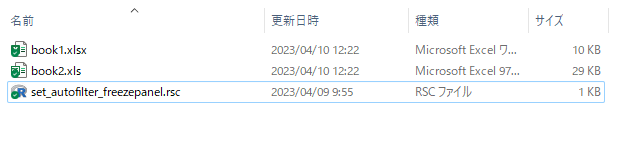
\includegraphics[width=0.8\textwidth,height=\textheight]{img/set_autofilter_freezepanel01.png}
\item
  実行前のエクセルのファイル\\
  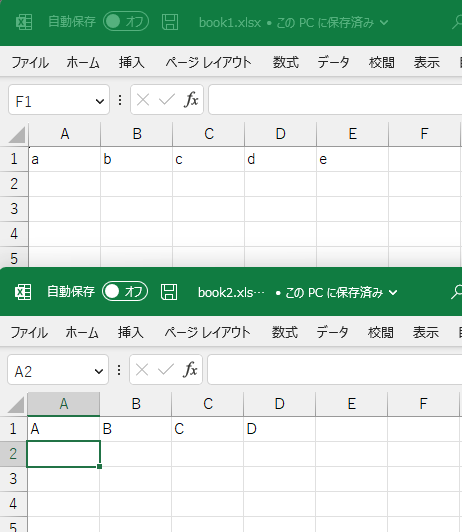
\includegraphics[width=0.6\textwidth,height=\textheight]{img/set_autofilter_freezepanel02.png}
\item
  set\_autofilter\_freezepanel.rsc をダブルクリックして実行すると,コマンドのウィンドウでプログラムが実行される.\\
  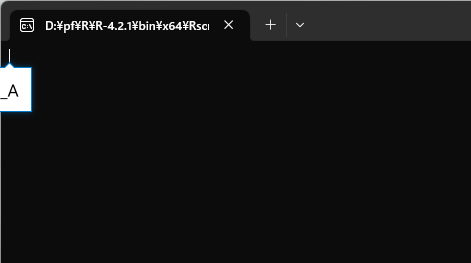
\includegraphics[width=0.6\textwidth,height=\textheight]{img/set_autofilter_freezepanel03.png}\\
  プログラムがオートフィルタを設定し,1行目と1列目でウィンドウ枠を固定する.
  複数ファイル・複数シートにも対応している.\\
  なお,初回実行時は,openxlsxパケージのダウンロードのため,少し時間がかかるかもしれない.
  2回目以降はファイル数が多すぎなければ,一瞬で処理されるはず.\\
  実行後のエクセルのファイル\\
  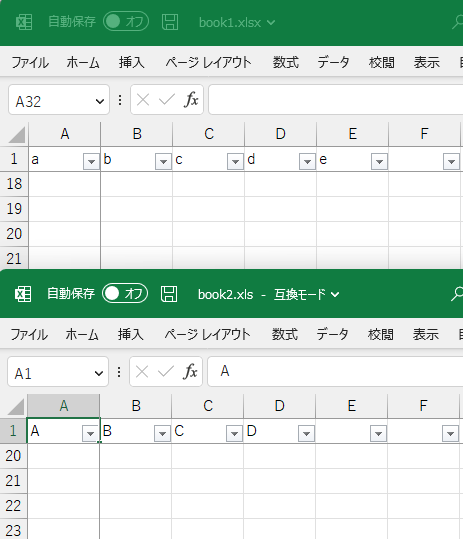
\includegraphics[width=0.6\textwidth,height=\textheight]{img/set_autofilter_freezepanel04.png}
\end{itemize}

\hypertarget{qpdf}{%
\section{qpdfでPDF操作}\label{qpdf}}

\hypertarget{ux6e96ux5099-14}{%
\subsection{準備}\label{ux6e96ux5099-14}}

いつものように,まずパッケージをインストールする.
qpdfはPDF操作のためのパッケージである.
著者作パッケージのであるautomaterをインストールするが,これはCRANには登録していない.
いずれはCRANに登録したいと思っているが,現段階ではGitHubで公開している.
そのため,install.packages()ではなく,remotes::install\_github()を使ってインストールする.

\begin{Shaded}
\begin{Highlighting}[]
\FunctionTok{install.packages}\NormalTok{(}\StringTok{"qpdf"}\NormalTok{)}
\FunctionTok{install.packages}\NormalTok{(}\StringTok{"devtools"}\NormalTok{)}
\NormalTok{remotes}\SpecialCharTok{::}\FunctionTok{install\_github}\NormalTok{(}\StringTok{"matutosi/automater"}\NormalTok{)}
\end{Highlighting}
\end{Shaded}

\begin{Shaded}
\begin{Highlighting}[]
\FunctionTok{library}\NormalTok{(tidyverse)}
\FunctionTok{library}\NormalTok{(qpdf)}
\FunctionTok{library}\NormalTok{(automater)}
\end{Highlighting}
\end{Shaded}

\hypertarget{qpdfux3067ux3067ux304dux308bux3053ux3068}{%
\subsection{qpdfでできること}\label{qpdfux3067ux3067ux304dux308bux3053ux3068}}

qpdfパッケージでは,PDFファイルのページ分割・抽出・結合・回転・圧縮・重ね合わせが可能である.
あくまでページ単位での操作で,PDFに含まれるテキスト自体の編集はできない.
ページ単位でのPDF操作は,Adobe AcrobatでなくてもCubePDF UtilityやPDFtkを使えば可能である.
PDFtkはコマンドラインでの操作も可能であるため,大量の操作をするには適している.
とはいえ,Rやそのパッケージで操作が自動化できればさらに便利である.

なお,PDF関連の他のパッケージとしてはpdftoolsがある.
pdftoolsではテキスト抽出,OCR(画像の文字認識,内部でtesseractパッケージを使用),PDFファイルの分割・結合(内部でqpdfパッケージの関数を使用),画像ファイルへの変換などができる.
また,Microsoft365Rを使えばPDFをワードに変換できる.
\protect\hyperlink{microsoft365r}{Microsoft365R}

余談だが,Rのパッケージはそれぞれ独自コードを持つ部分がある一方で,他のパッケージの関数をインポートしているものや,ラッパー関数を用意しているものなどがある.
例えば,automaterではそれ自体で有用な機能を持っているというよりは,他のパッケージを利用しやすくするためのラッパー関数の集合である.
そのため,automaterのコードをもとにして改良可能であり,各自で試してほしい.

\hypertarget{pdfux306eux5206ux5272}{%
\subsection{PDFの分割}\label{pdfux306eux5206ux5272}}

PDFの分割は非常に簡単である.
pdf\_split()関数にinput引数として分割するファイルを,output引数として出力パスを指定すれば良い.
パスワードが必要な場合は,引数passwordを指定する.

\begin{Shaded}
\begin{Highlighting}[]
  \CommentTok{\# wd \textless{}{-} "set\_your\_directory"}
  \CommentTok{\# setwd(wd)}
\NormalTok{review }\OtherTok{\textless{}{-}} 
\NormalTok{  curl}\SpecialCharTok{::}\FunctionTok{curl\_download}\NormalTok{(}
    \StringTok{"https://www.jstage.jst.go.jp/article/vegsci/31/2/31\_193/\_pdf/{-}char/ja"}\NormalTok{, }
\NormalTok{    fs}\SpecialCharTok{::}\FunctionTok{file\_temp}\NormalTok{(}\AttributeTok{ext =} \StringTok{"pdf"}\NormalTok{)}
\NormalTok{    )}
\NormalTok{split\_pdf }\OtherTok{\textless{}{-}}\NormalTok{ qpdf}\SpecialCharTok{::}\FunctionTok{pdf\_split}\NormalTok{(review)}
\FunctionTok{head}\NormalTok{(split\_pdf)}
\end{Highlighting}
\end{Shaded}

ファイル名の文字列のベクトルが返り値なので,それをもとにファイル名を変更すると実用的な自動化ができるだろう.

ページを指定した抽出も可能で,pdf\_subset()関数を使用する.
引数としてpagesを指定する以外は,pdf\_split()と同じ使い方である.

\begin{Shaded}
\begin{Highlighting}[]
  \CommentTok{\# 指定ページを抽出,create a new pdf with a subset of the input pages}
\FunctionTok{pdf\_subset}\NormalTok{(input, }\AttributeTok{pages =} \DecValTok{1}\NormalTok{, }\AttributeTok{output =} \ConstantTok{NULL}\NormalTok{, }\AttributeTok{password =} \StringTok{""}\NormalTok{)}
\end{Highlighting}
\end{Shaded}

以下の内容は,パッケージautomaterのinst/rscディレクトリにあるsplit\_qpdf.rscの内容である.
拡張子.rscをRscriptに関連付けすれば,split\_qpdf.rscと同じフォルダに保存したPDFファイルをsplit\_qpdf.rscをクリックするだけで分割できる.
拡張子の関連付けは,\protect\hyperlink{assoc}{スクリプトの関連付け}を参照して欲しい.

\begin{Shaded}
\begin{Highlighting}[]
\NormalTok{fs}\SpecialCharTok{::}\FunctionTok{path\_package}\NormalTok{(}\StringTok{"automater"}\NormalTok{, }\StringTok{"rsc"}\NormalTok{, }\StringTok{"split\_qpdf.rsc"}\NormalTok{)}
\end{Highlighting}
\end{Shaded}

\begin{verbatim}
## D:/pf/R/R-4.3.1/library/automater/rsc/split_qpdf.rsc
\end{verbatim}

\begin{Shaded}
\begin{Highlighting}[]
  \FunctionTok{readLines}\NormalTok{() }\SpecialCharTok{\%\textgreater{}\%}
  \FunctionTok{paste0}\NormalTok{(}\AttributeTok{collapse =} \StringTok{"}\SpecialCharTok{\textbackslash{}n}\StringTok{"}\NormalTok{) }\SpecialCharTok{\%\textgreater{}\%}
  \FunctionTok{cat}\NormalTok{()}
  \CommentTok{\# fs::path\_package("automater", "rsc", "split\_qpdf.rsc")}
  \CommentTok{\#   readtext::readtext(verbosity = 0) \%\textgreater{}\%}
  \CommentTok{\#   \textasciigrave{}[[\textasciigrave{}("text") \%\textgreater{}\%}
  \CommentTok{\#   cat()}
\end{Highlighting}
\end{Shaded}

具体的な方法は次のとおりである.

\begin{itemize}
\tightlist
\item
  split\_qpdf.rsc をディレクトリーに保存する\\
\item
  以下のコードで split\_qpdf.rsc をコピー可能
\end{itemize}

\begin{Shaded}
\begin{Highlighting}[]
\NormalTok{file }\OtherTok{\textless{}{-}} \StringTok{"split\_qpdf"}
\NormalTok{path }\OtherTok{\textless{}{-}} \StringTok{"c:/"} \CommentTok{\# set your path}
\NormalTok{automater}\SpecialCharTok{::}\FunctionTok{set\_rsc}\NormalTok{(file, path)}
\end{Highlighting}
\end{Shaded}

\begin{itemize}
\tightlist
\item
  拡張子 .rsc を Rscript.exe に関連付ける\\
\item
  分割したいPDFファイルを split\_qpdf.rsc と同じディレクトリにコピーする\\
\item
  split\_qpdf.rsc をクリックする\\
\item
  黒いウィンドウが開くので,しばらく待つ
\end{itemize}

split\_qpdf.rsc を初めて実行するときは,パッケージのインストールに時間がかかることがある.
出力ファイル名は以下のとおりである.

\begin{itemize}
\tightlist
\item
  入力:「original.pdf」(15ページ)\\
\item
  出力: ``original\_01.pdf'', ``original\_02.pdf'', \ldots, ``original\_15.pdf''
\end{itemize}

\hypertarget{pdfux306eux7d50ux5408}{%
\subsection{PDFの結合}\label{pdfux306eux7d50ux5408}}

結合させる場合は,input引数に結合させたいファイル名を指定する.
それ以外は,pdf\_split()と同様である.

\begin{Shaded}
\begin{Highlighting}[]
  \CommentTok{\# 結合,join several pdf files into one}
\FunctionTok{pdf\_combine}\NormalTok{(input, }\AttributeTok{output =} \ConstantTok{NULL}\NormalTok{, }\AttributeTok{password =} \StringTok{""}\NormalTok{)}
\end{Highlighting}
\end{Shaded}

特定のディレクトリ内のPDFファイルを1つのPDFファイルとして結合することを自動化するスクリプトは以下のとおりである.

\begin{Shaded}
\begin{Highlighting}[]
\NormalTok{fs}\SpecialCharTok{::}\FunctionTok{path\_package}\NormalTok{(}\StringTok{"automater"}\NormalTok{, }\StringTok{"rsc"}\NormalTok{, }\StringTok{"combine\_qpdf.rsc"}\NormalTok{)}
\end{Highlighting}
\end{Shaded}

\begin{verbatim}
## D:/pf/R/R-4.3.1/library/automater/rsc/combine_qpdf.rsc
\end{verbatim}

\begin{Shaded}
\begin{Highlighting}[]
  \FunctionTok{readLines}\NormalTok{() }\SpecialCharTok{\%\textgreater{}\%}
  \FunctionTok{paste0}\NormalTok{(}\AttributeTok{collapse =} \StringTok{"}\SpecialCharTok{\textbackslash{}n}\StringTok{"}\NormalTok{) }\SpecialCharTok{\%\textgreater{}\%}
  \FunctionTok{cat}\NormalTok{()}
\end{Highlighting}
\end{Shaded}

\begin{itemize}
\tightlist
\item
  combine\_qpdf.rsc をディレクトリに保存\\
\item
  以下のコードで、combine\_qpdf.rsc をコピー可能
\end{itemize}

\begin{Shaded}
\begin{Highlighting}[]
\NormalTok{file }\OtherTok{\textless{}{-}} \StringTok{"combine\_qpdf"}
\NormalTok{path }\OtherTok{\textless{}{-}} \StringTok{"c:/"} \CommentTok{\# set your path}
\NormalTok{automater}\SpecialCharTok{::}\FunctionTok{set\_rsc}\NormalTok{(file, path)}
\end{Highlighting}
\end{Shaded}

\begin{itemize}
\tightlist
\item
  拡張子 .rsc を Rscript.exe に関連付ける\\
\item
  結合したいPDFファイルを combine\_qpdf.rsc と同じディレクトリにコピーする\\
  ファイルの結合順はファイル名の順序と同じ\\
\item
  combine\_qpdf.rsc をクリックする\\
\item
  黒いウィンドウが開くので,しばらく待つ\\
  初めて実行するときは,パッケージのインストールに時間がかかることがある.\\
\item
  結合したファイル名は以下のとおりである.\\
  出力: 「combined\_``2020-11-27\_12\_00\_00.pdf''」(結合した日付・時刻)
\end{itemize}

PDFファイルの結合順はファイル名の順序と同じなので,\texttt{fs::dir\_ls()}でファイル名一覧を取得し,\texttt{file\_move()}で名前を変更する必要がある.
さらに,このあたりも自動化するには,ユーザからの入力を受け取り,それをもとにファイル名の順序を決めれば良い.

\begin{Shaded}
\begin{Highlighting}[]
  \CommentTok{\# wd \textless{}{-} "set\_your\_directory"}
  \CommentTok{\# setwd(wd)}
\FunctionTok{library}\NormalTok{(tidyverse)}
\NormalTok{input\_files }\OtherTok{\textless{}{-}} \ControlFlowTok{function}\NormalTok{(files)\{}
\NormalTok{  len }\OtherTok{\textless{}{-}} \FunctionTok{length}\NormalTok{(files) }\SpecialCharTok{\%\textgreater{}\%} \FunctionTok{log10}\NormalTok{() }\SpecialCharTok{\%\textgreater{}\%} \FunctionTok{ceiling}\NormalTok{()}
\NormalTok{  no }\OtherTok{\textless{}{-}}\NormalTok{ stringr}\SpecialCharTok{::}\FunctionTok{str\_pad}\NormalTok{(}\FunctionTok{seq}\NormalTok{(files), }\AttributeTok{width =}\NormalTok{ len, }\AttributeTok{side =} \StringTok{"left"}\NormalTok{)}
\NormalTok{  prompt }\OtherTok{\textless{}{-}} 
\NormalTok{    files }\SpecialCharTok{\%\textgreater{}\%}
    \FunctionTok{paste0}\NormalTok{(no, }\StringTok{": "}\NormalTok{, .) }\SpecialCharTok{\%\textgreater{}\%}
    \FunctionTok{paste0}\NormalTok{(}\AttributeTok{collapse =} \StringTok{"}\SpecialCharTok{\textbackslash{}n}\StringTok{"}\NormalTok{) }\SpecialCharTok{\%\textgreater{}\%}
    \FunctionTok{paste0}\NormalTok{(}\StringTok{"}\SpecialCharTok{\textbackslash{}n}\StringTok{結合するファイルを番号で指定してください(カンマ区切り).}\SpecialCharTok{\textbackslash{}n}\StringTok{  例:3,1,2}\SpecialCharTok{\textbackslash{}n}\StringTok{"}\NormalTok{) }\SpecialCharTok{\%\textgreater{}\%}
    \FunctionTok{cat}\NormalTok{()}
\NormalTok{  input\_order }\OtherTok{\textless{}{-}} 
    \FunctionTok{user\_input}\NormalTok{(prompt) }\SpecialCharTok{\%\textgreater{}\%}
\NormalTok{    stringr}\SpecialCharTok{::}\FunctionTok{str\_split}\NormalTok{(}\StringTok{","}\NormalTok{) }\SpecialCharTok{\%\textgreater{}\%}
    \FunctionTok{unlist}\NormalTok{() }\SpecialCharTok{\%\textgreater{}\%}
    \FunctionTok{as.numeric}\NormalTok{()}
\NormalTok{  files[input\_order]}
\NormalTok{\}}
\NormalTok{user\_input }\OtherTok{\textless{}{-}} \ControlFlowTok{function}\NormalTok{(prompt)\{}
  \ControlFlowTok{if}\NormalTok{ (}\FunctionTok{interactive}\NormalTok{()) \{}
    \FunctionTok{return}\NormalTok{(}\FunctionTok{readline}\NormalTok{(prompt))}
\NormalTok{  \} }\ControlFlowTok{else}\NormalTok{ \{}
    \FunctionTok{cat}\NormalTok{(prompt)}
    \FunctionTok{return}\NormalTok{(}\FunctionTok{readLines}\NormalTok{(}\StringTok{"stdin"}\NormalTok{, }\AttributeTok{n=}\DecValTok{1}\NormalTok{))}
\NormalTok{  \}}
\NormalTok{\}}

\NormalTok{files }\OtherTok{\textless{}{-}}\NormalTok{ fs}\SpecialCharTok{::}\FunctionTok{dir\_ls}\NormalTok{(}\AttributeTok{regexp =} \StringTok{"}\SpecialCharTok{\textbackslash{}\textbackslash{}}\StringTok{.pdf"}\NormalTok{)}
\NormalTok{input }\OtherTok{\textless{}{-}} \FunctionTok{input\_files}\NormalTok{(files)}
\NormalTok{input}

\NormalTok{automater}\SpecialCharTok{::}\FunctionTok{message\_to\_continue}\NormalTok{()}
\end{Highlighting}
\end{Shaded}

上のコードの\texttt{input\_files()}では,ファイル名の一覧からファイル数を取り出し,ファイル番号を画面表示用に桁揃えしている.
その後,ファイル番号とファイル名,さらにユーザへの註釈を結合して,プロンプトに表示するメッセージ文字列を生成する.
メッセージを\texttt{user\_input()}を用いて表示するとともに,ユーザからの入力を受け取る.
入力された文字列を数値にして,ファイルの順序を決めている.

このコードの\texttt{input}を\texttt{pdf\_combine(input)}として使えば,ユーザ入力をもとにしてPDFファイルを結合するスクリプトができる.
入力する番号が数個であれば,これでも良いがもっと多くのファイルになった場合は現実的には使いにくい.
多くのファイルを結合する場合は,以下のような方法で実装すると良いだろう.

\begin{itemize}
\tightlist
\item
  \texttt{fs::dir\_ls(regexp\ =\ "\textbackslash{}\textbackslash{}.pdf")}でファイル名の一覧を入手\\
\item
  一覧をもとに1行ごとに1つのファイル名のテキストファイルとして保存\\
\item
  テキストファイルをユーザが並び替える(Rでは並び替えが終わるまで待機)\\
\item
  並び替えが終われば,RでEnter(他のキーでもOK)を入力\\
\item
  テキストファイルを読み込み,\texttt{combine\_qpdf()}(\texttt{qpdf::pdf\_combine()}でもOK)でPDFを結合
\end{itemize}

\hypertarget{pdfux306eux5727ux7e2eux6700ux9069ux5316}{%
\subsection{PDFの圧縮・最適化}\label{pdfux306eux5727ux7e2eux6700ux9069ux5316}}

pdf\_compress()は圧縮や最適化(Linealize)をしてくれる.
最適化されていないPDFはファイルを全部読み込まないと表示できないのに対して,
最適化されたPDFは最後まで読み込みが完了しなくてもページ表示できる.
ネット上にある重いPDFを表示させる場合に特に役立つ.
使い方は次のとおりである.
詳細な説明は不要だろう.

\begin{Shaded}
\begin{Highlighting}[]
  \CommentTok{\# 圧縮,compress or linearize a pdf file}
  \CommentTok{\# 最適化する場合は,linearize = TRUE}
\FunctionTok{pdf\_compress}\NormalTok{(input, }\AttributeTok{output =} \ConstantTok{NULL}\NormalTok{, }\AttributeTok{linearize =} \ConstantTok{FALSE}\NormalTok{, }\AttributeTok{password =} \StringTok{""}\NormalTok{)}
\end{Highlighting}
\end{Shaded}

\hypertarget{pdfux3078ux306eux30daux30fcux30b8ux756aux53f7ux4ed8ux52a0}{%
\subsection{PDFへのページ番号付加}\label{pdfux3078ux306eux30daux30fcux30b8ux756aux53f7ux4ed8ux52a0}}

\texttt{pdf\_overlay\_stamp()}を使うと,PDFファイルに別のPDFファイルを重ね合わせることができる.

\begin{Shaded}
\begin{Highlighting}[]
  \CommentTok{\# automater::pdf\_overlay\_stamp()と同じ}
\NormalTok{pdf\_overlay\_stamp}
\end{Highlighting}
\end{Shaded}

引数\texttt{input}にはベースとなるPDFファイルを,\texttt{stamp}には重ね合わせるPDFファイルを指定する.
\texttt{stamp}として「部外秘」「資料1」などを記載したPDFファイルをあらかじめ準備しておく.
\texttt{input}の各ページに\texttt{stamp}の1ページ目が重ね合わせられる.

これだけでも十分便利な機能であるが,さらに便利に使いたい.
例えば,ベースのPDFファイルの各ページにページ番号を入力したい.
ページ番号でなくて別の通し番号を使いたいときもあるだろう.
例えば,学会の発表要旨集で左上に「A01」「A02」のような会場番号と通し番号を使うことが多い.
さらに欲をだして,重ね合わせの開始・終了ページを指定するようにしたい.

これらの内容を実行するコードは次のとおりである.

\begin{Shaded}
\begin{Highlighting}[]
\NormalTok{pdf\_overlay\_stamps\_each}
\end{Highlighting}
\end{Shaded}

\begin{verbatim}
## function (input, stamp, start = 1, end = NULL) 
## {
##     len_input <- qpdf::pdf_length(input)
##     len_stamp <- qpdf::pdf_length(stamp)
##     if (is.null(end)) {
##         end <- len_input
##     }
##     if (end < 0) {
##         end <- len_input + end
##     }
##     validate_page(len_input, len_stamp, start, end)
##     pages_inputs <- seq(to = len_input)
##     pages_pre <- if (start != 1) {
##         seq(to = start - 1)
##     }
##     else {
##         len_input + 1
##     }
##     pages_post <- if (end != len_input) {
##         seq(from = end + 1, to = len_input)
##     }
##     else {
##         len_input + 1
##     }
##     pages_body <- pages_inputs[-c(pages_pre, pages_post)]
##     inputs <- qpdf::pdf_split(input)
##     stamps <- qpdf::pdf_split(stamp)
##     out <- list()
##     for (i in seq_along(pages_body)) {
##         out[[i]] <- qpdf::pdf_overlay_stamp(inputs[pages_body[i]], 
##             stamps[i])
##     }
##     out <- stats::na.omit(c(inputs[pages_pre], unlist(out), inputs[pages_post]))
##     outfile <- qpdf::pdf_combine(out, "out.pdf")
##     file.remove(inputs)
##     file.remove(stamps)
##     file.remove(out[pages_body])
##     return(outfile)
## }
## <bytecode: 0x0000022ef26aaab0>
## <environment: namespace:automater>
\end{verbatim}

\texttt{pdf\_overlay\_stamps\_each()}の引数には,\texttt{input},\texttt{stamp},\texttt{start},\texttt{end}がある.
\texttt{input}と\texttt{stamp}はqpdfの他の関数と同様の引数で,ファイルのパスを文字列で指定する.
\texttt{start}と\texttt{end}は,\texttt{input}での重ね合わせ対象とするページ数の開始・終了ページで,整数で指定する.
最後からのページ数とするには,\texttt{end}を負の数で指定する.

関数の主な構成は以下のとおりである.
- \texttt{input}と\texttt{stamp}のページ数を取得\\
- \texttt{start}や\texttt{end}との整合性を\texttt{validate\_page()}で確認\\
- 重ね合わせ対象よりも前(\texttt{pages\_pre}),後ろ(\texttt{pages\_post}),重ね合わせの対象のページ(\texttt{pages\_body})を取得\\
- \texttt{pdf\_split()}で\texttt{input}と\texttt{stamp}を1ページごとに分割\\
- \texttt{pages\_body}の部分のみ,\texttt{stamp}の各ページを重ね合わせ\\
- combine\_pdf()で使うためのファイル名を結合(\texttt{pages\_pre},\texttt{pages\_body},\texttt{pages\_post})\\
- combine\_pdf()でファイルの結合\\
- 使用後のファイルを削除\\
- 結合したファイル名を返す

なお,ページ番号と学会でのセッション番号を付与するためのラッパー関数として,それぞれ\texttt{pdf\_overlay\_page\_num()}と\texttt{pdf\_overlay\_session\_num()}がある.
\texttt{pdf\_overlay\_page\_num()}は,\texttt{input}のPDFだけ指定すれば全ページに番号を付加し,\texttt{start}と\texttt{end}が指定可能である.
ただし,最大ページ数は100ページである.
\texttt{pdf\_overlay\_session\_num()}は,さらに\texttt{session}を指定して「A01」のような番号を左上に付加する.

\begin{Shaded}
\begin{Highlighting}[]
\FunctionTok{pdf\_overlay\_page\_num}\NormalTok{(input, }\AttributeTok{start =} \DecValTok{1}\NormalTok{, }\AttributeTok{end =} \ConstantTok{NULL}\NormalTok{)}
\FunctionTok{pdf\_overlay\_session\_num}\NormalTok{(input, }\AttributeTok{start =} \DecValTok{1}\NormalTok{, }\AttributeTok{end =} \ConstantTok{NULL}\NormalTok{, }\AttributeTok{session =} \StringTok{"a"}\NormalTok{)}
\end{Highlighting}
\end{Shaded}

パッケージautomaterのpdfフォルダには,ページ番号と学会でのセッション番号を付加するためのPDFファイル(すべてA4版)がある.

\begin{itemize}
\tightlist
\item
  00\_page.pdf\\
\item
  00\_sn\_a.pdf,00\_sn\_b.pdf,00\_sn\_p.pdf
\end{itemize}

ページ番号は,下部に「-1-」などの表記があり100ページ分からなる.
セッション番号は,左上に「A01」(A会場を想定)「B01」「P01」(ポスター会場を想定)などの表記があり,50番までが入っている.
それぞれのtexソースファイルも保存されている.
texを使うのが難しければ,ワードなどで同様の書式のファイルを作成したものをPDFとして保存すれば良い.

\hypertarget{ux305dux306eux4ed6ux306eux95a2ux6570-1}{%
\subsection{その他の関数}\label{ux305dux306eux4ed6ux306eux95a2ux6570-1}}

これまでで説明した以外に,qpdfには\texttt{pdf\_length()}と\texttt{pdf\_rotate\_pages()}がある.
\texttt{pdf\_length()}は入力したPDFファイルのページ数を返す.
\texttt{pdf\_rotate\_pages()}はPDFファイルのページを90度単位で回転できる.
\texttt{angle}で時計回りの角度を指定する.
\texttt{relative}が\texttt{TRUE}のときは入力時点での角度からの相対的な角度で回転し,\texttt{FALSE}のときは\texttt{angle\ =\ 0}のときは縦長で\texttt{angle\ =\ 90}のときは横長になる.

\begin{Shaded}
\begin{Highlighting}[]
\FunctionTok{pdf\_length}\NormalTok{(input, }\AttributeTok{password =} \StringTok{""}\NormalTok{)   }
\FunctionTok{pdf\_rotate\_pages}\NormalTok{(input, pages, }\AttributeTok{angle =} \DecValTok{90}\NormalTok{, }\AttributeTok{relative =} \ConstantTok{FALSE}\NormalTok{, }\AttributeTok{output =} \ConstantTok{NULL}\NormalTok{, }\AttributeTok{password =} \StringTok{""}\NormalTok{)   }
\end{Highlighting}
\end{Shaded}

\hypertarget{pdftools}{%
\subsection{pdftoolsでテキストの取り出し}\label{pdftools}}

pdftoolsパッケージでは,テキスト抽出,OCR(画像の文字認識),PDFファイルの分割・結合,画像ファイルへの変換などができる.
このうち,OCRではtesseractパッケージを,PDFの分割・結合ではqpdfパッケージの関数を使っており,直接それぞれのパッケージを使うのと基本的には同じ,画像ファイルへの変換はmagickパッケージで可能である.
そのため,ここでは他のパッケージでは実装していないテキスト抽出を説明する.
なお,テキスト抽出にはpopplerを使っている.
Windows版のpdftoolsパッケージではpopplerが含まれているのでパッケージのインストールだけで使用可能である.
MacやLinuxでは,popplerを別途インストールしなければならない.
popplerのインストール方法は以下を参考にして欲しい.

\url{https://docs.ropensci.org/pdftools/}

まずは,パッケージのインストールと呼び出しを実行する.

\begin{Shaded}
\begin{Highlighting}[]
\FunctionTok{install.packages}\NormalTok{(}\StringTok{"pdftools"}\NormalTok{)}
\end{Highlighting}
\end{Shaded}

\begin{Shaded}
\begin{Highlighting}[]
\FunctionTok{library}\NormalTok{(pdftools)}
\end{Highlighting}
\end{Shaded}

関数\texttt{pdf\_text()}にPDFファイルのパスを指定すれば,テキストを抽出した結果が得られる.
1ページごとの内容が文字列のベクトルになっている.

\begin{Shaded}
\begin{Highlighting}[]
  \CommentTok{\# https://docs.ropensci.org/pdftools/}
\NormalTok{url }\OtherTok{\textless{}{-}} \StringTok{"http://arxiv.org/pdf/1403.2805.pdf"}
\NormalTok{destfile }\OtherTok{\textless{}{-}}\NormalTok{ fs}\SpecialCharTok{::}\FunctionTok{file\_temp}\NormalTok{(}\AttributeTok{ext =} \StringTok{"pdf"}\NormalTok{)}
\NormalTok{curl}\SpecialCharTok{::}\FunctionTok{curl\_download}\NormalTok{(url, destfile)}
\NormalTok{txt }\OtherTok{\textless{}{-}}\NormalTok{ pdftools}\SpecialCharTok{::}\FunctionTok{pdf\_text}\NormalTok{(destfile)}
\NormalTok{tibble}\SpecialCharTok{::}\FunctionTok{as\_tibble}\NormalTok{(txt)}
\end{Highlighting}
\end{Shaded}

\begin{verbatim}
## # A tibble: 29 x 1
##    value                                                                        
##    <chr>                                                                        
##  1 "                                              The jsonlite Package: A Pract~
##  2 "JSON with R. We refer to Nolan and Temple Lang (2014) for a comprehensive i~
##  3 "homogenous. And indeed, some implementations will now return a list instead~
##  4 "The alternative to class-based method dispatch is to use type-based encodin~
##  5 "2       Converting between JSON and R classes\n\nThis section lists example~
##  6 "encoding. However, the problem with encoding missing values as strings is t~
##  7 "limitations as text based formats such as CSV.\n\n\n2.1.3      Special case~
##  8 "is assuming an array, the application will likely break. Any consumer or cl~
##  9 "We expect this representation will be the most intuitive to interpret, also~
## 10 "colnames(x) <- c(\"Treatment A\", \"Treatment B\")\nprint(x)\n\n        Tre~
## # i 19 more rows
\end{verbatim}

文字列内の\texttt{\textbackslash{}n}は改行を示しているが,そのままでは読みにくい.
\texttt{\textbackslash{}n}で改行して画面で表示するには\texttt{cat()}を使う.

\begin{Shaded}
\begin{Highlighting}[]
\FunctionTok{cat}\NormalTok{(txt[}\DecValTok{1}\NormalTok{])  }\CommentTok{\# [1]で1ページ目}
\end{Highlighting}
\end{Shaded}

\hypertarget{RDCOMClient}{%
\section{RDCOMClientでMS WordやExcelと他形式と相互変換する}\label{RDCOMClient}}

RDCOMClientはWindowsに特化したパッケージであるが,これを使うとMS WordやExcelの操作が可能である.
ここでは,WordおよびExcelを他のファイル形式に変換したり,その逆の方法を紹介する.
また,操作対象のWordやExcelがインストールされている必要がある.

\hypertarget{ux6e96ux5099-15}{%
\subsection{準備}\label{ux6e96ux5099-15}}

CRANには登録されておらず,ウェブページかGitHubからインストールする.
\texttt{install.packages()}でインストールする場合は,バイナリなので比較的時間が早いが,Rのバージョンによってはうまくインストールできないかもしれない.
\texttt{install\_github()}の場合は,コンパイルするのに少し時間がかかる.

\begin{Shaded}
\begin{Highlighting}[]
  \CommentTok{\# どちらか一方でうまくいけばOK}
\NormalTok{utils}\SpecialCharTok{::}\FunctionTok{install.packages}\NormalTok{(}\StringTok{"RDCOMClient"}\NormalTok{, }\AttributeTok{repos =} \StringTok{"http://www.omegahat.net/R"}\NormalTok{, }\AttributeTok{type =} \StringTok{"win.binary"}\NormalTok{)}
\NormalTok{remotes}\SpecialCharTok{::}\FunctionTok{install\_github}\NormalTok{(}\StringTok{"omegahat/RDCOMClient"}\NormalTok{)}
\NormalTok{remotes}\SpecialCharTok{::}\FunctionTok{install\_github}\NormalTok{(}\StringTok{"matutosi/automater"}\NormalTok{)}
\end{Highlighting}
\end{Shaded}

\begin{Shaded}
\begin{Highlighting}[]
\FunctionTok{library}\NormalTok{(tidyverse)}
\FunctionTok{library}\NormalTok{(RDCOMClient)}
\FunctionTok{library}\NormalTok{(automater)}
\end{Highlighting}
\end{Shaded}

\hypertarget{ux30c9ux30adux30e5ux30e1ux30f3ux30c8ux306eux5f62ux5f0fux5909ux63db}{%
\subsection{ドキュメントの形式変換}\label{ux30c9ux30adux30e5ux30e1ux30f3ux30c8ux306eux5f62ux5f0fux5909ux63db}}

\begin{Shaded}
\begin{Highlighting}[]
\NormalTok{convert\_docs}
\end{Highlighting}
\end{Shaded}

\begin{verbatim}
## function (path, format) 
## {
##     if (fs::path_ext(path) == format) {
##         return(invisible(path))
##     }
##     no <- switch(format, docx = 11, pdf = 17, xps = 19, html = 20, 
##         rtf = 23, txt = 25)
##     path <- normalizePath(path)
##     suppressWarnings({
##         converted <- normalizePath(path_convert(path, pre = "converted_", 
##             ext = format))
##     })
##     wordApp <- RDCOMClient::COMCreate("Word.Application")
##     wordApp[["Visible"]] <- TRUE
##     wordApp[["DisplayAlerts"]] <- FALSE
##     doc <- wordApp[["Documents"]]$Open(path, ConfirmConversions = FALSE)
##     doc$SaveAs2(converted, FileFormat = no)
##     doc$close()
##     return(invisible(converted))
## }
## <bytecode: 0x00000165a599ee78>
## <environment: namespace:automater>
\end{verbatim}

\texttt{convert\_docs()}の中でファイルの読み込み・保存でファイル名を指定する.
その際に\texttt{normalizePath()}を使う必要がある.
この部分を別の関数に置き換えても大丈夫かと考えて,\texttt{fs::path\_norm()}を使ってみたところエラーになった.
このように,コードを改善しようとする場合は,作業の結果としてうまく動作しないことがよくり,注意が必要である.

\texttt{doc\$SaveAs2()}の\texttt{FileFormat\ =\ no}で保存形式をそれに対応する数値で指定している.
このあたりは,試行錯誤の結果である.
もしかしたら他の形式での保存が可能なのかもしれないが,確実に変換できるのは以下の5つである.

\begin{itemize}
\tightlist
\item
  pdf:PDF
\item
  xps:XML Paper Specification(xmlベースファイル形式)\\
\item
  html:HTML\\
\item
  rtf:リッチテキスト\\
\item
  txt:テキスト
\end{itemize}

なお,\texttt{convert\_docs()}の実行時には,MS Wordを起動してその機能としてファイルの読み込み・保存をする.
そのため,MS Wordがインストールされていないと,この関数は使えない.

複数のdocxファイルを圧縮したzipファイルがあり,ファイル解凍,PDFへの変換,1つのPDFファイルへの結合をするようなコードは以下のとおりである.
結合時の順序はファイル名の順序に従う.
そのため,PDFファイルでのファイル順を踏まえて,docxの命名規則を決める必要がある.

\begin{itemize}
\tightlist
\item
  \texttt{unzip()}で解凍\\
\item
  \texttt{fs::dir\_ls()}でファイル名取得\\
\item
  \texttt{convert\_docs()}で形式変換\\
\item
  \texttt{qpdf\_combine()}で結合
\end{itemize}

\#\#スプレッドシートの形式変換

\hypertarget{microsoft365r}{%
\section{Microsoft365Rでメールを一斉送信する}\label{microsoft365r}}

\hypertarget{outlookux3067ux8907ux6570ux30e1ux30fcux30ebux9001ux4fe1ux3092ux4e00ux6589ux9001ux4fe1}{%
\subsection{Outlookで複数メール送信を一斉送信}\label{outlookux3067ux8907ux6570ux30e1ux30fcux30ebux9001ux4fe1ux3092ux4e00ux6589ux9001ux4fe1}}

複数人に全く同じメールを送る場合は,TOやCCに複数の電子メールアドレスを入力すれば良い.
また,宛先を知られるのがよろしくないときは,BCCに送信先のアドレスを,TOに自分のアドレスを入れておけば問題ない.
このとき,送り先の全員に全く同じ内容,同じ添付ファイルであればメールは1つ作成すれば問題ない.

でも,個々の人に対して少しだけ違う内容のメールを送りたいときとか,添付ファイルを別々のものにしたいときがある.
また,単純なことだが,宛先が「みなさま」よりは,「田中様」のように宛先だけでも変更したいというときもある.
何かお願いをするときには,「みなさま」よりも直接名前を書いたほうが結構効果が高い.
例えば,学会での投票のお願いなどは,MLに流すより個別メールの方が確実だ.

そのようなとき,いちいちメールを作成・編集していると面倒だし,間違いのもとになる.
名前を中途半端に修正して,3箇所のうち1箇所だけ別の人の名前にしたり,日付と曜日があっていないなどの間違いは日常茶飯事だ.
このような間違いをなくすには,個別に変更する部分と全体で統一するところを分けておき,あとはパソコンを使ってうまくつなぎ合わせる.
でも,このように作成したメールの本文や宛先をいちいちコピー\&ペーストするのは,手間がかかるし,個々にも作業のミスが入り込む余地が大きい.

\hypertarget{ux30a4ux30f3ux30b9ux30c8ux30fcux30ebux3068ux521dux671fux8a2dux5b9a}{%
\subsubsection{インストールと初期設定}\label{ux30a4ux30f3ux30b9ux30c8ux30fcux30ebux3068ux521dux671fux8a2dux5b9a}}

この操作は,最初に1回だけ実行すればOK.

\begin{Shaded}
\begin{Highlighting}[]
  \CommentTok{\# インストール}
\FunctionTok{install.packages}\NormalTok{(}\StringTok{"Microsoft365R"}\NormalTok{)}
  \CommentTok{\# パッケージの読み込み}
\end{Highlighting}
\end{Shaded}

\begin{Shaded}
\begin{Highlighting}[]
\FunctionTok{library}\NormalTok{(tidyverse)}
\FunctionTok{library}\NormalTok{(Microsoft365R)}
 \CommentTok{\# 会社など組織で契約している場合}
\NormalTok{Microsoft365R}\SpecialCharTok{::}\FunctionTok{get\_business\_outlook}\NormalTok{()}
 \CommentTok{\# 個人利用の場合}
  \CommentTok{\# Microsoft365R::get\_personal\_outlook()}
\end{Highlighting}
\end{Shaded}

\hypertarget{ux3068ux308aux3042ux3048ux305aux4f7fux3046}{%
\subsubsection{とりあえず使う}\label{ux3068ux308aux3042ux3048ux305aux4f7fux3046}}

まずは,試しにメールを作って送ってみる.

\begin{Shaded}
\begin{Highlighting}[]
 \CommentTok{\# 会社などで組織で契約している場合}
\NormalTok{outlook }\OtherTok{\textless{}{-}}\NormalTok{ Microsoft365R}\SpecialCharTok{::}\FunctionTok{get\_business\_outlook}\NormalTok{()}
 \CommentTok{\# 個人利用の場合}
  \CommentTok{\# outlook \textless{}{-} Microsoft365R::get\_personal\_outlook()}

  \CommentTok{\# 個別にemailを送る場合}
  \CommentTok{\# メール作成のみ}
  \CommentTok{\# メールはoutlookの下書きフォルダにも保存されている}
\NormalTok{em }\OtherTok{\textless{}{-}} 
\NormalTok{  outlook}\SpecialCharTok{$}\FunctionTok{create\_email}\NormalTok{(}
    \AttributeTok{body =} \StringTok{"Hello from R}\SpecialCharTok{\textbackslash{}n}\StringTok{Hello from R}\SpecialCharTok{\textbackslash{}n}\StringTok{"}\NormalTok{, }
    \AttributeTok{subject =} \StringTok{"Hello"}\NormalTok{,}
    \AttributeTok{to =} \StringTok{"matutosi@gmail.com"}\NormalTok{, }
    \AttributeTok{cc =} \StringTok{"matutosi@konan{-}wu.ac.jp"}
\NormalTok{  )}

  \CommentTok{\# メール送信}
\NormalTok{em}\SpecialCharTok{$}\FunctionTok{send}\NormalTok{()}

  \CommentTok{\# outlookの下書きフォルダからメールを取り出す}
\NormalTok{drafts }\OtherTok{\textless{}{-}}\NormalTok{ outlook}\SpecialCharTok{$}\FunctionTok{get\_drafts}\NormalTok{()}\SpecialCharTok{$}\FunctionTok{list\_emails}\NormalTok{()}
  \CommentTok{\# 下書きフォルダのメール一覧}
\NormalTok{drafts}
  \CommentTok{\# 下書きフォルダのメールの1つ目を送信}
\NormalTok{drafts[[}\DecValTok{1}\NormalTok{]]}\SpecialCharTok{$}\FunctionTok{send}\NormalTok{()}

  \CommentTok{\# 受信トレイのメール一覧}
\NormalTok{inbox }\OtherTok{\textless{}{-}}\NormalTok{ outlook}\SpecialCharTok{$}\FunctionTok{get\_inbox}\NormalTok{()}\SpecialCharTok{$}\FunctionTok{list\_emails}\NormalTok{()}
  \CommentTok{\# 受信トレイの1つ目の内容}
\NormalTok{inbox[[}\DecValTok{1}\NormalTok{]]}
\end{Highlighting}
\end{Shaded}

\hypertarget{ux30e1ux30fcux30ebux306eux4e00ux6589ux9001ux4fe1}{%
\subsubsection{メールの一斉送信}\label{ux30e1ux30fcux30ebux306eux4e00ux6589ux9001ux4fe1}}

宛先や本文をエクセルに入力しておき,そこからデータを抽出して一斉にメールを送信できる.

\begin{itemize}
\tightlist
\item
  送信: send(必須) 1: 送信する,0: 下書きに保存
\item
  宛先: to(必須)\\
\item
  CC: cc(任意)\\
\item
  BCC: bcc(任意)\\
\item
  件名: subject(必須でないが,入力推奨)\\
\item
  本文: body(必須でないが,入力推奨)\\
\item
  添付ファイル: attachment(任意)
\end{itemize}

宛先が入力されていないとメールは送信できない.
CCとBCCは任意.\\
件名と本文はなくても送信できるが,両方とも何もないとメールの意味がない.\\
添付ファイルがあれば,ファイル名を指定.
複数ファイルを添付するときは,カンマでパス(ファイル名)を区切る.
絶対パスで指定すると間違いは少ない.

\begin{Shaded}
\begin{Highlighting}[]
  \CommentTok{\# 宛先や本文をエクセルで作成しておき}
  \CommentTok{\#   一斉にメールを作成・送信する場合}

  \CommentTok{\# 関数の読み込み}
\FunctionTok{source}\NormalTok{(}\StringTok{"https://gist.githubusercontent.com/matutosi/bed00135698c8e3d2c49ef08d12eef9c/raw/6acc2de844eeeab03aaf36f2391e223d621b36a8/outlook.R"}\NormalTok{)}

\NormalTok{outlook }\OtherTok{\textless{}{-}}\NormalTok{ Microsoft365R}\SpecialCharTok{::}\FunctionTok{get\_business\_outlook}\NormalTok{()}
  \CommentTok{\# エクセルファイルの内容}
  \CommentTok{\#   working directoryにファイルがない場合は,}
  \CommentTok{\#   絶対パス("c:/user/documents/outlook.xlsx"など)で指定}
\NormalTok{path }\OtherTok{\textless{}{-}} \StringTok{"outlook.xlsx"}
  \CommentTok{\# メール作成・送信}
\FunctionTok{create\_email}\NormalTok{(path, outlook, }\AttributeTok{send =} \ConstantTok{TRUE}\NormalTok{)}

  \CommentTok{\# メール作成のみ}
  \CommentTok{\#   "send = FALSE" にすれば,メールを作成して下書きに保存}
\FunctionTok{create\_email}\NormalTok{(path, outlook, }\AttributeTok{send =} \ConstantTok{FALSE}\NormalTok{)}
\end{Highlighting}
\end{Shaded}

\hypertarget{officer}{%
\section{officerでWordやEscelの内容を編集する}\label{officer}}

\hypertarget{ux6e96ux5099-16}{%
\subsection{準備}\label{ux6e96ux5099-16}}

例によってまずはパッケージをインストールする.
日付のデータを扱うためのlubridateとさらにそのラッパーを使うので,automaterを読み込む.

\begin{Shaded}
\begin{Highlighting}[]
\FunctionTok{install.packages}\NormalTok{(}\StringTok{"officer"}\NormalTok{)}
\end{Highlighting}
\end{Shaded}

\begin{verbatim}
## -- Attaching core tidyverse packages ------------------------ tidyverse 2.0.0 --
## v dplyr     1.1.2     v readr     2.1.4
## v forcats   1.0.0     v stringr   1.5.0
## v ggplot2   3.4.2     v tibble    3.2.1
## v lubridate 1.9.2     v tidyr     1.3.0
## v purrr     1.0.1     
## -- Conflicts ------------------------------------------ tidyverse_conflicts() --
## x dplyr::filter() masks stats::filter()
## x dplyr::lag()    masks stats::lag()
## i Use the conflicted package (<http://conflicted.r-lib.org/>) to force all conflicts to become errors
\end{verbatim}

\hypertarget{officerux3068officeverse}{%
\subsection{officerとofficeverse}\label{officerux3068officeverse}}

\hypertarget{ux8907ux6570ux306eux30efux30fcux30c9ux6587ux66f8ux306eux6587ux5b57ux5217ux3092ux4e00ux62ecux7f6eux63db}{%
\subsection{複数のワード文書の文字列を一括置換}\label{ux8907ux6570ux306eux30efux30fcux30c9ux6587ux66f8ux306eux6587ux5b57ux5217ux3092ux4e00ux62ecux7f6eux63db}}

多くのプログラマは,普段はそれぞれの好みのテキストエディタを使っていいるだろう.
私はWindowsでは古典的なエディタである秀丸エディタを長らく使っている.
キー割り当てのカスタマイズや自分用の細かなマクロがあるので,今さらエディタを変更できない.
ノートパソコンではThinkPadをずっと使っているので,キーボード自体も変更できない.
これを変更すると作業効率が悪くなってしまう.
そのため,デスクトップパソコンでもThinkPadキーボードを愛用している.

このようにエディタとキーボードだけでパソコンの作業が完了すれば良いのだが,仕事上はワードで文書を作成しなければならないことがある.
ワードは余計なおせっかいをたくさんしてくれるので,不要なことはしないように設定している.
それでも,できればワードでの作業は最小限にしたいのが本音である.
起動に時間はかかるし,置換で使える正規表現がちょっと変だからである.

Rからワード文書内の文字列を置換すれば,ワードを起動する手間が省略できる.
また,正規表現を使った置換や複数の組み合わせの置換もできる.
さらに,「AをB」に「BをA」にという入れ替えも,プログラムで途中に別の文字列への置き換えで実現できる.
このとき途中で使う文字列が元の文書内にないことは必須条件であるが,これもプログラムで確認可能である.
もちろん,複数ファイルでの置換やファイル名を正規表現で指定することもできる.

\hypertarget{ux7f6eux63dbux306eux30b3ux30fcux30c9ux306eux4f8b}{%
\subsubsection{置換のコードの例}\label{ux7f6eux63dbux306eux30b3ux30fcux30c9ux306eux4f8b}}

\begin{Shaded}
\begin{Highlighting}[]
  \CommentTok{\# コードの動作確認}

  \CommentTok{\# https://ardata{-}fr.github.io/officeverse/index.html}
  \CommentTok{\# pkg \textless{}{-} "D:/matu/work/ToDo/automater/R"}
  \CommentTok{\# devtools::load\_all(pkg)}

  \CommentTok{\# fs::path\_package("")}
  \CommentTok{\# replacement \textless{}{-} readr::read\_tsv("replacement.txt", header = TRUE)}
  \CommentTok{\# ls("package:tibble")}

\FunctionTok{library}\NormalTok{(tidyverse)}
\FunctionTok{library}\NormalTok{(officer)}
\FunctionTok{library}\NormalTok{(lubridate)}
  \CommentTok{\# library(automater)}
\NormalTok{a }\OtherTok{\textless{}{-}} 
  \FunctionTok{read\_docx}\NormalTok{() }\SpecialCharTok{\%\textgreater{}\%}
\NormalTok{  officer}\SpecialCharTok{::}\FunctionTok{body\_add\_par}\NormalTok{(}\StringTok{"置換前,変換前,へんかん,ヘンカン"}\NormalTok{) }\SpecialCharTok{\%\textgreater{}\%}
  \FunctionTok{print}\NormalTok{(fs}\SpecialCharTok{::}\FunctionTok{path\_temp}\NormalTok{(}\StringTok{"a.docx"}\NormalTok{))}
\NormalTok{b }\OtherTok{\textless{}{-}} 
  \FunctionTok{read\_docx}\NormalTok{() }\SpecialCharTok{\%\textgreater{}\%}
\NormalTok{  officer}\SpecialCharTok{::}\FunctionTok{body\_add\_par}\NormalTok{(}\StringTok{"置換前,変換前,へんかん,ヘンカン"}\NormalTok{) }\SpecialCharTok{\%\textgreater{}\%}
  \FunctionTok{print}\NormalTok{(fs}\SpecialCharTok{::}\FunctionTok{path\_temp}\NormalTok{(}\StringTok{"b.docx"}\NormalTok{))}
\NormalTok{fs}\SpecialCharTok{::}\FunctionTok{path\_dir}\NormalTok{(a) }\SpecialCharTok{\%\textgreater{}\%}
  \FunctionTok{shell.exec}\NormalTok{()}

\NormalTok{replacement }\OtherTok{\textless{}{-}} 
\NormalTok{  tibble}\SpecialCharTok{::}\FunctionTok{tribble}\NormalTok{(}
    \SpecialCharTok{\textasciitilde{}}\NormalTok{file          , }\SpecialCharTok{\textasciitilde{}}\NormalTok{old\_value, }\SpecialCharTok{\textasciitilde{}}\NormalTok{new\_value,}
\NormalTok{    a              , }\StringTok{"置換前"}\NormalTok{  , }\StringTok{"置換後"}\NormalTok{  ,}
\NormalTok{    b              , }\StringTok{"変換前"}\NormalTok{  , }\StringTok{"変換後"}\NormalTok{  ,}
    \FunctionTok{paste0}\NormalTok{(a,}\StringTok{","}\NormalTok{,b), }\StringTok{"へんかん"}\NormalTok{, }\StringTok{"変換"}\NormalTok{    )}

\NormalTok{replacement }\OtherTok{\textless{}{-}} 
\NormalTok{  replacement }\SpecialCharTok{\%\textgreater{}\%}
  \FunctionTok{expand\_file}\NormalTok{() }\SpecialCharTok{\%\textgreater{}\%}
\NormalTok{  dplyr}\SpecialCharTok{::}\FunctionTok{filter}\NormalTok{(}\SpecialCharTok{!}\NormalTok{stringr}\SpecialCharTok{::}\FunctionTok{str\_detect}\NormalTok{(file, }\StringTok{"replaced}\SpecialCharTok{\textbackslash{}\textbackslash{}}\StringTok{\_"}\NormalTok{))}

\FunctionTok{replace\_docs}\NormalTok{(replacement)}
\end{Highlighting}
\end{Shaded}

\hypertarget{ux5e74ux6708ux65e5ux306eux66f4ux65b0}{%
\subsection{年月日の更新}\label{ux5e74ux6708ux65e5ux306eux66f4ux65b0}}

毎年同じような文書を作成しているが,年だけを更新しなければならないことは多いだろう.
手作業で日付を更新すると,どうしても間違いが混入する.
単純な見間違いや入力間違いもあれば,日付を変更して曜日を変更し忘れる,あるいは日付を変更し忘れることをやってしまいがちだ.
このような更新作業も,Wordの検索・置換の機能で可能だし,Rから特定の日付を別の日付に変換できる.

いっそのことなら,日付を文書内で自動的に取得して日付あるいは曜日を更新できれば楽ができる.
例えば,「2023年4月10日(月)」を2024年に変更することを考えよう.
何番目の何曜日かで日付が決まっているなら,2023年4月10日は第2月曜日である.
この場合は,2024年4月の第2月曜日は「2024年4月8日(月)」なので,「2023年4月10日(月)」を「2024年4月8日(月)」に置換する.
一方,日付固定なら「2024年4月10日(水)」に置換する.

さらに,求めた日が日曜日の場合は前日の土曜日あるいは月曜日にずらすとか,10月1日の前後3日以内の火曜日のような法則でも可能である.
祝日との関連で日付を決定することもあるだろう.
そのようなときは,祝日データをあわせてコードに入れれば良い.
とにかく,作業の手順が決まっていれば,プログラムによる自動化できる.

ここではlubridateを活用して,ワード文書の日付を更新する方法を扱う.
lubridateで日付固定あるいは位置固定のときでの翌年の年月日を求める方法は以下を参考にして欲しい.

\protect\hyperlink{lubridate}{lubridateで日付・時刻を扱う}

\hypertarget{ux6d3bux7528ux4f8b-1}{%
\subsubsection{活用例}\label{ux6d3bux7528ux4f8b-1}}

ワード文書内の日付は,正規表現を用いて入手できる.

それぞれの曜日なし版が考えられ,月と日が1桁の時に「04」のようにパディング(桁合わせ)されていることもあるだろう.
これらは正規表現によって対応可能である.
日付っぽい表記のすべてを含もうとするとややこしいが,よく使う日付表記であれば網羅できるだろう.
年表記が2桁の場合,半角や全角のスペースを途中に含んだり,「()」の半角・全角の違いなどの表現揺れもあり得る.
表記揺れを修正するための置換や削除などは,stringr(あるいはbase)の関数で対応できる.

\begin{Shaded}
\begin{Highlighting}[]
  \CommentTok{\# Wordファイルを開く}
  \CommentTok{\# 文字列の取得}
  \CommentTok{\# 日付の一覧抽出}
  \CommentTok{\# 日付の置換}
  \CommentTok{\# Wordの保存}

  \CommentTok{\# library(automater)}
  \CommentTok{\# library(moranajp)}
\FunctionTok{library}\NormalTok{(tidyverse)}
\FunctionTok{library}\NormalTok{(officer)}
\FunctionTok{library}\NormalTok{(lubridate)}

  \CommentTok{\# 準備}
\NormalTok{x }\OtherTok{\textless{}{-}} 
  \StringTok{"23年1月1日(月),2023年1月1日(月),2023年10月10日(月),}
\StringTok{  2月2日(月),12月22日(月),2023/1/1(月),2023/10/10(月),}
\StringTok{  2/2(月),12/22(月),23年1月1日,2023年1月1日,}
\StringTok{  2023年10月10日,2月2日,12月22日,2023/1/1,2023/10/10,}
\StringTok{  2/2,12/22"}
\NormalTok{date\_x }\OtherTok{\textless{}{-}} \FunctionTok{extract\_date}\NormalTok{(x)}
\NormalTok{date\_doc }\OtherTok{\textless{}{-}} \FunctionTok{print}\NormalTok{(fs}\SpecialCharTok{::}\FunctionTok{path\_temp}\NormalTok{(}\StringTok{"date.docx"}\NormalTok{))}

\NormalTok{doc }\OtherTok{\textless{}{-}} \FunctionTok{read\_docx}\NormalTok{()}
\NormalTok{doc }\OtherTok{\textless{}{-}} \FunctionTok{body\_add\_par}\NormalTok{(doc, }\StringTok{"日付置換の例"}\NormalTok{)}
\ControlFlowTok{for}\NormalTok{(d }\ControlFlowTok{in}\NormalTok{ date\_x)\{}
\NormalTok{  doc }\OtherTok{\textless{}{-}} \FunctionTok{body\_add\_par}\NormalTok{(doc, d)}
  \CommentTok{\#   doc \textless{}{-} body\_add\_fpar(doc, fpar(ftext(d, fp\_text(color = "red"))))}
\NormalTok{\}}
\FunctionTok{write\_docx}\NormalTok{(doc, date\_doc)}
\NormalTok{fs}\SpecialCharTok{::}\FunctionTok{path\_dir}\NormalTok{(date\_doc) }\SpecialCharTok{\%\textgreater{}\%}
  \FunctionTok{shell.exec}\NormalTok{()}

  \CommentTok{\# 読み込み}
\NormalTok{doc }\OtherTok{\textless{}{-}} \FunctionTok{read\_docx}\NormalTok{(date\_doc)}


\NormalTok{automater}\SpecialCharTok{::}\FunctionTok{format\_ymd}\NormalTok{(x)}

  \CommentTok{\# ls("package:officer")}
  \CommentTok{\# ls("package:moranajp")}
\end{Highlighting}
\end{Shaded}


\end{document}
